%!TEX TS-program = xelatex
%!TEX encoding = UTF-8 Unicode

% ------------------------------------------------------------------------------
% customize the headers with fancyhdr package
% ------------------------------------------------------------------------------
\usepackage{fancyhdr}
\fancyhf{}
\fancyhead[LE]{\leftmark}
\fancyhead[RO]{\nouppercase{\rightmark}}
\fancyfoot[LE,RO]{\thepage}
\pagestyle{fancy}

% ------------------------------------------------------------------------------
% Index package
% ------------------------------------------------------------------------------
% \usepackage{makeidx}
% \makeindex

% ------------------------------------------------------------------------------
% load hyperref to use hyperlinks
% ------------------------------------------------------------------------------
\usepackage[colorlinks=true,linkcolor=blue]{hyperref}
\usepackage[all]{hypcap}  % Be sure to call this package after loading hyperref.

% ------------------------------------------------------------------------------
% Glossaries, must be after hyperref
% ------------------------------------------------------------------------------
\usepackage[xindy,toc]{glossaries}
\makeglossaries{}

% ------------------------------------------------------------------------------
% load tocbibind to add contents,list of figures, list of tables and
% bibliography into the toc
% ------------------------------------------------------------------------------
\usepackage{tocbibind}

% ------------------------------------------------------------------------------
% Needed to load images
% ------------------------------------------------------------------------------
\usepackage{graphicx}
\graphicspath{ {images/} }   % where to look for images

\usepackage{color}
\usepackage{tabularx}
\usepackage{multirow}

\usepackage{framed}

% ------------------------------------------------------------------------------
% for code example
% ------------------------------------------------------------------------------
\usepackage{listings}

\definecolor{syntax_comment}{rgb}{0.72,0.14,0.15}	% red
\definecolor{syntax_key}{rgb}{0.05,0.5,0.07}
\definecolor{syntax_gray}{rgb}{0.5,0.5,0.5}
\definecolor{syntax_string}{rgb}{0.58,0,0.82}	% mauve
\definecolor{background}{rgb}{0.975,0.975,0.975}

\lstset{ %
  backgroundcolor=\color{background},   % choose the background color; you must add \usepackage{color} or \usepackage{xcolor}
  basicstyle=\scriptsize\ttfamily, % the size of the fonts that are used for the code
  breakatwhitespace=false,         % sets if automatic breaks should only happen at whitespace
  breaklines=true,                 % sets automatic line breaking
  captionpos=b,                    % sets the caption-position to bottom
  commentstyle=\itshape\color{syntax_comment},    % comment style
%  deletekeywords={...},            % if you want to delete keywords from the given language
%  escapeinside={\%*}{*)},          % if you want to add LaTeX within your code
  extendedchars=true,              % lets you use non-ASCII characters; for 8-bits encodings only, does not work with UTF-8
%  frame=single,                    % adds a frame around the code
  keepspaces=true,                 % keeps spaces in text, useful for keeping indentation of code (possibly needs columns=flexible)
  keywordstyle=\color{syntax_key},       % keyword style
%  language=Octave,                 % the language of the code
%  otherkeywords={*,...},           % if you want to add more keywords to the set
  numbers=none,                    % where to put the line-numbers; possible values are (none, left, right)
  numbersep=5pt,                   % how far the line-numbers are from the code
  numberstyle=\tiny\color{syntax_gray}, % the style that is used for the line-numbers
  rulecolor=\color{black},         % if not set, the frame-color may be changed on line-breaks within not-black text (e.g. comments (green here))
  showspaces=false,                % show spaces everywhere adding particular underscores; it overrides 'showstringspaces'
  showstringspaces=false,          % underline spaces within strings only
  showtabs=false,                  % show tabs within strings adding particular underscores
  stepnumber=1,                    % the step between two line-numbers. If it's 1, each line will be numbered
  stringstyle=\color{syntax_string},     % string literal style
  tabsize=2                        % sets default tabsize to 2 spaces
%  title=\lstname                   % show the filename of files included with \lstinputlisting; also try caption instead of title
}

% ------------------------------------------------------------------------------
% for long and nice table
% ------------------------------------------------------------------------------
\usepackage{longtable}
\usepackage{booktabs}
\usepackage{ltxtable}

% ------------------------------------------------------------------------------
% for compact item list
% ------------------------------------------------------------------------------
\usepackage{paralist}

% ------------------------------------------------------------------------------
% Math - Warning: before cjkfonts (xeCJK) and other package loads fontspec
% ------------------------------------------------------------------------------
\usepackage{amsmath}
\usepackage{amsfonts}
\usepackage{amssymb}

% font selection for mathematics with XeLaTeX, MUST after amsfonts
\usepackage{mathspec}
% \setmathsfont(Digits,Latin,Greek)[Numbers={Lining,Proportional}]{Minion Pro}

% There's no italic sans-serif math font by default, but it's needed in this book
% follow: http://tex.stackexchange.com/questions/77640/bold-italic-and-sans-serif-math-symbols
% to define a \mathsfit{} macro
\DeclareMathAlphabet{\mathsfit}{\encodingdefault}{\sfdefault}{m}{sl}
\SetMathAlphabet{\mathsfit}{bold}{\encodingdefault}{\sfdefault}{bx}{sl}

% ------------------------------------------------------------------------------
% Localization setting
% ------------------------------------------------------------------------------
% file: localization.tex

% load cjkfonts and set Source Han Sans SC as the default CJK fonts:
\usepackage[default,mdseries=Light,bfseries=Medium]{cjkfonts}

\usepackage{titlesec}

\titleformat{\chapter}[display]
  {\bfseries\huge}%
  {\huge 第 \thechapter{} 章}%
  {10 pt}%
  {\bfseries\huge}%

\renewcommand{\contentsname}{目录}
\renewcommand{\indexname}{索引}

% Redefine \emph to be both bold and italic, better in chinese document
\let\emph\relax
%\DeclareTextFontCommand{\emph}{\bfseries\em} % bold and italic
\DeclareTextFontCommand{\emph}{\bfseries} % just bold

\usepackage{indentfirst}


% Set Roboto and Source Code Pro, which are installed with TexLive, for western
% fonts:
% file: westernfonts.tex

\newfontfamily\SourceCodePro{SourceCodePro}[
  UprightFont=*-Light,
  BoldFont=*-Medium,
  ItalicFont=*-LightIt,
  BoldItalicFont=*-MediumIt]

\newfontfamily\SourceSerifPro{SourceSerifPro}[
  UprightFont=*-Light,
  BoldFont=*-Semibold]

\newcommand{\serif}[0]{\SourceSerifPro}
 
\setmonofont{SourceCodePro}[
  UprightFont=*-Light,
  BoldFont=*-Medium,
  ItalicFont=*-LightIt,
  BoldItalicFont=*-MediumIt]


\usepackage{setspace}
\onehalfspacing{}

%\usepackage{tikz} % load TikZ/PGF
%\usetikzlibrary{circuits.logic.US,positioning,decorations.pathreplacing,mindmap,backgrounds,math}
\usepackage{pgfplots} % load PDFPlots
%\pgfplotsset{compat=yourversion}

% ------------------------------------------------------------------------------
% Load glossaries
% ------------------------------------------------------------------------------
%% glossaries

%% Chapter 1

\newglossaryentry{perceptron}{
  name={感知机},
  description={\emph{Perceptron}}
}

\newglossaryentry{sigmoid-neuron}{
  name={S 型神经元},
  description={\emph{Sigmoid Neuron}}
}

\newglossaryentry{sigmoid-func}{
  name={S 型函数},
  description={\emph{Sigmoid Function}}
}

\newglossaryentry{sgd}{
  name={随机梯度下降},
  description={\emph{Stochastic Gradient Descent}}
}

\newglossaryentry{weight}{
  name={权重},
  description={\emph{Weight}}
}

\newglossaryentry{bias}{
  name={偏置},
  description={\emph{Bias}}
}

\newglossaryentry{threshold}{
  name={阈值},
  description={\emph{Threshold}}
}

\newglossaryentry{epoch}{
  name={迭代期},
  description={\emph{Epoch}}
}

\newglossaryentry{mini-batch}{
  name={小批量数据},
  description={\emph{Mini-batch}}
}

\newglossaryentry{hidden-layer}{
  name={隐藏层},
  description={\emph{Hidden Layer}}
}

\newglossaryentry{mlp}{
  name={多层感知机},
  description={\emph{Multilayer Perceptron}}
}

\newglossaryentry{rnn}{
  name={循环神经网络},
  description={\emph{Recurrent Neural Network(s)}}
}

\newglossaryentry{cost-func}{
  name={代价函数},
  description={\emph{Cost Function}}
}

\newglossaryentry{learning-rate}{
  name={学习速率},
  description={\emph{Learning Rate}}
}

\newglossaryentry{bp}{
  name={反向传播},
  description={\emph{Backpropagation}}
}

\newglossaryentry{svm}{
  name={支持向量机},
  description={\emph{Support Vector Machine}}
}

\newglossaryentry{deep-neural-networks}{
  name={深度神经网络},
  description={\emph{Deep Neural Networks}}
}

\newglossaryentry{error}{
  name={误差},
  description={\emph{Error}}
}

\newglossaryentry{reln}{
  name={修正线性神经元},
  description={\emph{Rectified Linear Neuron}}
}

\newglossaryentry{relu}{
  name={修正线性单元},
  description={\emph{Rectified Linear Unit}}
}

\newglossaryentry{softmax}{
  name={柔性最大值},
  description={\emph{Softmax}}
}

\newglossaryentry{softmax-func}{
  name={柔性最大值函数},
  description={\emph{Softmax Function}}
}

\newglossaryentry{log-likelihood}{
  name={对数似然},
  description={\emph{Log-likelihood}}
}

\newglossaryentry{regularization}{
  name={正则化},
  description={\emph{Regularization}}
}

\newglossaryentry{weight-decay}{
  name={权重衰减},
  description={\emph{Weight Decay}}
}

\newglossaryentry{regularization-term}{
  name={正则化项},
  description={\emph{Regularization Term}}
}

\newglossaryentry{lrf}{
  name={局部感受野},
  description={\emph{Local Receptive Fields}}
}

\newglossaryentry{shared-weights}{
  name={共享权重},
  description={\emph{Shared Weights}}
}

\newglossaryentry{pooling}{
  name={池化},
  description={\emph{Pooling}}
}

\newglossaryentry{cnn}{
  name={卷积神经网络},
  description={\emph{Convolutional Neural Networks}}
}

\newglossaryentry{idui}{
  name={意图驱动的用户接口},
  description={\emph{Intention-driven User Interface}}
}

\newglossaryentry{tanh}{
  name={双曲正切},
  description={\emph{Tanh},(发音为 “tanch”)}
}

\newglossaryentry{tanh-func}{
  name={双曲正切函数},
  description={\emph{Tanh Function}}
}

\newglossaryentry{tanh-neuron}{
  name={双曲正切神经元},
  description={\emph{Tanh Neuron}}
}

\newglossaryentry{hyperbolic-tangent}{
  name={双曲正切},
  description={\emph{Hyperbolic Tangent}}
}

\newglossaryentry{hyper-params}{
  name={超参数},
  description={\emph{Hyper-parameters}}
}

\newglossaryentry{lstm}{
  name={长短期记忆单元},
  description={\emph{Long Short-term Memory Units}}
}

\newglossaryentry{dbn}{
  name={深度信念网络},
  description={\emph{Deep Belief Network(s)}}
}
	
%% ------

\newglossaryentry{logistic-regression}{
  name={Logistic 回归},
  description={\emph{Logistic Regression}}
}

\newglossaryentry{naive-bayes}{
  name={朴素贝叶斯},
  description={\emph{naive Bayes}}
}

\newglossaryentry{representations}{
  name={表征},
  description={\emph{Representations},表征是信息的呈现方式}
}

\newglossaryentry{rep-learning}{
  name={表征学习},
  description={\emph{Representation Learning}}
}

\newglossaryentry{autoencoder}{
  name={自编码器},
  description={\emph{Autoencoder (s)}}
}

\newglossaryentry{encoder}{
  name={编码器},
  description={\emph{encoder}}
}

\newglossaryentry{decoder}{
  name={解码器},
  description={\emph{decoder}}
}

\newglossaryentry{fov}{
  name={变化因素},
  description={\emph{factors of variation}}
}

%% Chapter 2

\newglossaryentry{scalar}{
  name={标量},
  description={scalar}
}

\newglossaryentry{scalars}{
  name={标量},
  description={Scalars}
}

\newglossaryentry{vec}{
  name={向量},
  description={vector}
}

\newglossaryentry{vecs}{
  name={向量},
  description={Vectors}
}

\newglossaryentry{matrix}{
  name={矩阵},
  description={matrix}
}

\newglossaryentry{matrices}{
  name={矩阵},
  description={Matrices}
}

\newglossaryentry{tensor}{
  name={张量},
  description={tensor}
}

\newglossaryentry{tensors}{
  name={张量},
  description={Tensors}
}

\newglossaryentry{transpose}{
  name={转置},
  description={transpose}
}

\newglossaryentry{main-diag}{
  name={主对角线},
  description={main diagonal}
}

\newglossaryentry{broadcasting}{
  name={广播},
  description={broadcasting}
}

\newglossaryentry{matrix-product}{
  name={矩阵积},
  description={matrix product}
}

\newglossaryentry{element-product}{
  name={按元素乘积},
  description={element-wise product}
}

\newglossaryentry{hadamard-product}{
  name={阿达玛乘积},
  description={Hadamard product}
}

\newglossaryentry{dot-product}{
  name={点乘},
  description={dot product}
}

\newglossaryentry{matrix-inversion}{
  name={矩阵求逆},
  description={matrix inversion}
}

\newglossaryentry{identity-matrix}{
  name={单位矩阵},
  description={identity matrix}
}

\newglossaryentry{linear-comb}{
  name={线性组合},
  description={linear combination}
}

\newglossaryentry{span}{
  name={生成空间},
  description={span}
}

\newglossaryentry{column-space}{
  name={列空间},
  description={column space}
}

\newglossaryentry{range}{
  name={范围},
  description={range}
}

\newglossaryentry{linear-dep}{
  name={线性相关},
  description={linear dependence}
}

\newglossaryentry{linearly-dep}{
  name={线性无关},
  description={linearly dependent}
}

\newglossaryentry{linearly-indep}{
  name={线性无关},
  description={linearly independent}
}

\newglossaryentry{linear-indep}{
  name={线性无关},
  description={linear independent}
}

\newglossaryentry{square}{
  name={方的},
  description={square}
}

\newglossaryentry{singular}{
  name={奇异矩阵},
  description={singular}
}

\newglossaryentry{norm}{
  name={范数},
  description={norm}
}

\newglossaryentry{tri-inequal}{
  name={三角不等式},
  description={triangle inequality}
}

\newglossaryentry{eu-norm}{
  name={欧几里德范数},
  description={Euclidean norm}
}

\newglossaryentry{max-norm}{
  name={最大值范数},
  description={max norm}
}

\newglossaryentry{fr-norm}{
  name={弗罗贝尼乌斯范数},
  description={Frobenius norm}
}

\newglossaryentry{diag}{
  name={对角线},
  description={Diagonal}
}

\newglossaryentry{symmetric}{
  name={对称},
  description={symmetric}
}

\newglossaryentry{unit-vec}{
  name={单位向量},
  description={unit vector}
}

\newglossaryentry{unit-norm}{
  name={单位范数},
  description={unit norm}
}

\newglossaryentry{ortho}{
  name={正交的},
  description={orthogonal}
}

\newglossaryentry{orthonormal}{
  name={标准正交的},
  description={orthonormal}
}

\newglossaryentry{orthonormal-matrix}{
  name={正交矩阵},
  description={orthonormal matrix}
}

\newglossaryentry{eigen-decompos}{
  name={特征分解},
  description={eigendecomposition}
}

\newglossaryentry{eigen-vec}{
  name={特征向量},
  description={eigenvector}
}

\newglossaryentry{eigen-vecs}{
  name={特征向量},
  description={eigenvectors}
}

\newglossaryentry{eigen-val}{
  name={特征值},
  description={eigenvalue}
}

\newglossaryentry{eigen-vals}{
  name={特征值},
  description={eigenvalues}
}

\newglossaryentry{left-eigen-vec}{
  name={左特征向量},
  description={left eigenvector}
}

\newglossaryentry{positive-definite}{
  name={正定矩阵},
  description={positive definite}
}

\newglossaryentry{positive-semidefinite}{
  name={半正定矩阵},
  description={positive semidefinite}
}

\newglossaryentry{negative-definite}{
  name={负定矩阵},
  description={negative definite}
}

\newglossaryentry{negative-semidefinite}{
  name={半负定矩阵},
  description={negative semidefinite}
}

\newglossaryentry{svd}{
  name={奇异值分解},
  description={singular value decomposition}
}

\newglossaryentry{singular-vecs}{
  name={奇异向量},
  description={singular vectors}
}

\newglossaryentry{singular-vals}{
  name={奇异值},
  description={singular values}
}

\newglossaryentry{singular-val}{
  name={奇异值},
  description={singular value}
}

\newglossaryentry{left-singular-vecs}{
  name={左奇异向量},
  description={left-singular vectors}
}

\newglossaryentry{right-singular-vecs}{
  name={右奇异向量},
  description={right-singular vectors}
}

\newglossaryentry{moore-penrose-pseudoinverse}{
  name={摩尔--彭若斯广义逆},
  description={Moore-Penrose pseudoinverse}
}

\newglossaryentry{pca}{
  name={主成分分析},
  description={principal components analysis}
}

%% Chapter 4

\newglossaryentry{overflow}{
  name={溢出},
  description={overflow}
}

\newglossaryentry{underflow}{
  name={下溢},
  description={underflow}
}

\newglossaryentry{cond-num}{
  name={条件数},
  description={condition number}
}

\newglossaryentry{obj-func}{
  name={目标函数},
  description={objective function}
}

\newglossaryentry{criterion}{
  name={准则},
  description={criterion, criterion funciton 准则函数}
}

\newglossaryentry{loss-func}{
  name={损失函数},
  description={loss function}
}

\newglossaryentry{err-func}{
  name={误差函数},
  description={error function}
}

\newglossaryentry{gradient-descent}{
  name={梯度下降},
  description={gradient descent}
}

\newglossaryentry{critical-points}{
  name={临界点},
  description={critical points}
}

\newglossaryentry{stationary-points}{
  name={驻点},
  description={stationary points}
}

\newglossaryentry{local-min}{
  name={局部最小值},
  description={local minimum}
}

\newglossaryentry{local-max}{
  name={局部最大值},
  description={local maximum}
}

\newglossaryentry{saddle-points}{
  name={鞍点},
  description={saddle points}
}

\newglossaryentry{global-min}{
  name={全局最小值},
  description={global minimum}
}

\newglossaryentry{partial-derivatives}{
  name={偏导数},
  description={partial derivatives}
}

\newglossaryentry{gradient}{
  name={梯度},
  description={gradient}
}

\newglossaryentry{directional-derivative}{
  name={方向导数},
  description={directional derivative}
}

\newglossaryentry{steepest-descent}{
  name={最陡下降法},
  description={method of steepest descent}
}

\newglossaryentry{line-search}{
  name={线搜索},
  description={line search}
}

\newglossaryentry{hill-climbing}{
  name={爬山算法},
  description={hill climbing}
}

\newglossaryentry{jacobian-matrix}{
  name={雅可比矩阵},
  description={Jacobian matrix}
}

\newglossaryentry{second-derivative}{
  name={二阶导数},
  description={second derivative}
}

\newglossaryentry{curvature}{
  name={曲率},
  description={curvature}
}

\newglossaryentry{hessian-matrix}{
  name={海森矩阵},
  description={Hessian matrix}
}

\newglossaryentry{second-derivative-test}{
  name={二阶导数检测},
  description={second derivative test}
}

%% Chapter 12

\newglossaryentry{warps}{
  name={线程束},
  description={\emph{Warps},同时运行的一组线程的称呼}
}

\newglossaryentry{overfitting}{
  name={过度拟合},
  description={\emph{Overfitting},过度拟合,过拟合,过适}
}

\newglossaryentry{overtraining}{
  name={过度训练},
  description={\emph{Overtraining}}
}

\newglossaryentry{generalization_error}{
  name={泛化误差},
  description={\emph{Generalization error},泛化误差}
}

\newglossaryentry{dropout}{
  name={弃权},
  description={\emph{Dropout}, 弃权}
}

\newglossaryentry{bdt}{
  name={提高决策树},
  description={\emph{Boosted decision trees}}
}

\newglossaryentry{gcn}{
  name={全局对比度归一化},
  description={\emph{Global contrast normalization}, 全局对比度归一化}
}

\newglossaryentry{mode}{
  name={众数},
  description={\emph{mode}, 众数}
}


% file: plots.tex
% used for plotting learning curve in chapter 3

% learn cost curve of a single sigmoid neutron with quadratic cost function
\newcommand{\quadraticCostLearning}[4]{
  \begin{tikzpicture}[
    inner sep=0pt,
    minimum size=10mm,
    background rectangle/.style={
      draw=gray!25,
      fill=gray!10,
      rounded corners
    },
    show background rectangle]

    \coordinate (origin) at (0,0);
    \coordinate(x) at (3.5,0);
    \coordinate(y) at (0,2.5);

    \node(i) [above=4 of origin,xshift=-5mm] {\footnotesize Input: $1.0$};
    \node(n) [right=2 of i,circle,draw] {};
    \node(epoch) [right=of x,xshift=-1cm] {\footnotesize Epoch};
    \node(cost) [left=of y,xshift=1cm] {\footnotesize Cost};

    \draw[->] (origin) to (x);
    \draw[->] (origin) to (y);

    %\draw[blue,thick,domain=0:2] plot (\x, {(\x*\x / 2)});

    \tikzmath{                  % Do not contain blank line
      function sigmoid(\z) {
        return 1/(1 + exp(- \z));
      };
      function sigmoid_neutron(\w,\b) {
        return sigmoid(\w + \b);
      };
      function quad_cost(\a) {         % the quadratic cost function
        return (\a * \a)/2;
      };
      function quad_cost_derivative(\a) {
        return \a * \a * (1-\a);
      };
      \w = #1;                % start weight
      \b = #2;                % start bias
      \e = #3;                % eta, learning rate
      \y = 0;
      \a = sigmoid_neutron(\w,\b);
      \dt = quad_cost_derivative(\a);
      \xo = 0;
      \yo = quad_cost(\a);
      integer \x;
      if #4 > 0 then {
        for \x in {1,...,#4}{  % epoches
          \a = sigmoid_neutron(\w,\b);
          \dt = quad_cost_derivative(\a);
          \w = \w - \e * \dt;
          \b = \b - \e * \dt;
          \y = quad_cost(\a);
          {\draw[blue,thick] (\xo/100,\yo*5) -- (\x/100,\y*5);};
          \xo = \xo + 1;
          \yo = \y;
        };
        {\draw (\x/100,0) -- node[below] {\footnotesize $\x$} (\x/100,-0.1);};
      };
      {
        \draw[->] (i) to node (w) [below] {
          \scriptsize
          \pgfkeys{/pgf/number format/.cd,showpos,fixed,fixed zerofill,precision=2,use period}
          $w = \pgfmathprintnumber{\w}$
        } (n);
        \node(b) [below,xshift=5mm] at (n.south) {
          \scriptsize
          \pgfkeys{/pgf/number format/.cd,showpos,fixed,fixed zerofill,precision=2,use period}
          $b = \pgfmathprintnumber{\b}$
        };
        \node(o) [right=of n] {
          \footnotesize
          \pgfkeys{/pgf/number format/.cd,fixed,fixed zerofill,precision=2,use period}
          Output: $\pgfmathprintnumber{\a}$
        };
        \draw[->] (n) to (o);
      };
    }

  \end{tikzpicture}%
}

% learn cost curve of a single sigmoid neutron with cross entropy cost function
\newcommand{\crossEntropyCostLearning}[4]{
  \begin{tikzpicture}[
    inner sep=0pt,
    minimum size=10mm,
    background rectangle/.style={
      draw=gray!25,
      fill=gray!10,
      rounded corners
    },
    show background rectangle]

    \coordinate (origin) at (0,0);
    \coordinate(x) at (3.5,0);
    \coordinate(y) at (0,2.5);

    \node(i) [above=4 of origin,xshift=-5mm] {\footnotesize Input: $1.0$};
    \node(n) [right=2 of i,circle,draw] {};
    \node(epoch) [right=of x,xshift=-1cm] {\footnotesize Epoch};
    \node(cost) [left=of y,xshift=1cm] {\footnotesize Cost};

    \draw[->] (origin) to (x);
    \draw[->] (origin) to (y);

    %\draw[blue,thick,domain=0:2] plot (\x, {(\x*\x / 2)});

    \tikzmath{                  % Do not contain blank line
      function sigmoid(\z) {
        return 1/(1 + exp(- \z));
      };
      function sigmoid_neutron(\w,\b) {
        return sigmoid(\w + \b);
      };
      function cross_entropy_cost(\a) {         % the quadratic cost function
        return -ln(1 - \a);
      };
      function cross_entropy_cost_derivative(\a) {
        return 1/(1 - \a);
      };
      \w = #1;                % start weight
      \b = #2;                % start bias
      \e = #3;                % eta, learning rate
      \y = 0;
      \a = sigmoid_neutron(\w,\b);
      \dt = cross_entropy_cost_derivative(\a);
      \xo = 0;
      \yo = cross_entropy_cost(\a);
      integer \x;
      if #4 > 0 then {
        for \x in {1,...,#4}{  % epoches
          \a = sigmoid_neutron(\w,\b);
          \dt = cross_entropy_cost_derivative(\a);
          \w = \w - \e * \dt;
          \b = \b - \e * \dt;
          \y = cross_entropy_cost(\a);
          {\draw[blue,thick] (\xo/100,\yo*5) -- (\x/100,\y*5);};
          \xo = \xo + 1;
          \yo = \y;
        };
        {\draw (\x/100,0) -- node[below] {\footnotesize $\x$} (\x/100,-0.1);};
      };
      {
        \draw[->] (i) to node (w) [below] {
          \scriptsize
          \pgfkeys{/pgf/number format/.cd,showpos,fixed,fixed zerofill,precision=2,use period}
          $w = \pgfmathprintnumber{\w}$
        } (n);
        \node(b) [below,xshift=5mm] at (n.south) {
          \scriptsize
          \pgfkeys{/pgf/number format/.cd,showpos,fixed,fixed zerofill,precision=2,use period}
          $b = \pgfmathprintnumber{\b}$
        };
        \node(o) [right=of n] {
          \footnotesize
          \pgfkeys{/pgf/number format/.cd,fixed,fixed zerofill,precision=2,use period}
          Output: $\pgfmathprintnumber{\a}$
        };
        \draw[->] (n) to (o);
      };
    }

  \end{tikzpicture}%
}


% ------------------------------------------------------------------------------
% The document body
% ------------------------------------------------------------------------------

\begin{document}

% file: title.tex

\begin{titlepage}
\begin{center}
  \hfill\\
  \vspace{1cm}
  % title of this document
  {\fontsize{36pt}{40pt}\NotoSansSCBold{} 神经网络与深度学习}\\
  \vspace{1em}
  {\LARGE\RobotoRegular{} \href{http://neuralnetworksanddeeplearning.com/index.html}{Neural Networks and Deep Learning}}\\
  \vspace{1cm}

  % borrow the code from http://latex-community.org/know-how/513-tikz-math
  \begin{tikzpicture}[scale=.06pt]
    \tikzmath{
      % --------------------------
      % the parameters of the tree
      % --------------------------
      \power=2.5; % the scale base factor
      \deviation=44.5; % the angle between the 3 child edges
      \numsteps=5; % number of levels
      let \startcolor=magenta; % the start color
      let \endcolor=black; % the end color
      % -------------------------------------------------------------------------
      % the function that draw one edge and call itself to draw the 3 child edges
      % -------------------------------------------------------------------------
      function Branch(\x,\y,\rotate,\step){
        \step=\step-1; % stops drawing if step < 0
        if (\step >= 0) then {
          \mix = int(100*\step/(\numsteps-1)); % the color mix parameter is in [0,100]
          \scale = \power^\step; % the scale factor
          { % "print" the tikz command that draw the edge
            \draw[shift={(\x pt,\y pt)}, rotate=\rotate, scale=\scale,
                  color=\startcolor!\mix!\endcolor, line width=\scale*.1 pt,
                  line cap=round]
              (0,0)--(1,0) coordinate(newbase);
          };
          coordinate \b; \b1 = (newbase); % the new base point
          for \a in {-\deviation,0,\deviation}{
            Branch(\bx1,\by1,mod(\rotate+\a,360),\step); % draw one child edge
          };
        };
      };
      % ----------------------
      % draw the four branches
      % ----------------------
      for \angle in {0,45,...,360}{
        Branch(0,0,\angle,\numsteps);
      };
    }
  \end{tikzpicture}
  
  \vspace{1cm}
  {\LARGE (美)\href{http://michaelnielsen.org/}{Michael Nielsen} 著}\\
  \vspace{1cm}
  {\Large
    \begin{tabular}{rl}
      \href{mailto:xhzhu.nju@gmail}{Xiaohu Zhu} & \multirow{2}{*}{译} \\
      \href{mailto:zhanggyb@gmail.com}{Freeman Zhang} & \\
    \end{tabular}
  }\\
  \vfill
  {\large \today}\\
  \vspace{1em}
  {\Huge\textcolor{red}{Early Preview}}
\end{center}
\end{titlepage}


\frontmatter

%\maketitle
% file: copyright.tex

\chapter{版权}

本书英文原版地址
为:
\href{http://neuralnetworksanddeeplearning.com/}{http://neuralnetworksanddeeplearning.com/}
。

在学术著作中请引用英文原文为:Michael A. Nielsen, ``Neural Networks and Deep
Learning'', Determination Press, 2015。

英文版及本书采
用 \href{http://creativecommons.org/licenses/by-nc/3.0/deed.en_GB}{Creative
  Commons Attribution-NonCommercial 3.0 Unported License} 许可协议。这意味着你可
以自由地拷贝、分发、扩展本书内容,但不得出售。如果你对商业用途感兴趣,英文版请联
系\href{mailto:mn@michaelnielsen.org}{作者},中文版请联
系\hyperref[sec:TranslationTeam]{翻译团队}。


\tableofcontents
%\listoffigures
%\listoftables

\pagebreak

% file: author.tex

\chapter{关于作者}
\label{ch:Author}

\begin{minipage}{0.7\linewidth}
\textbf{Michael Nielsen} 是一位量子物理学家、科学作家、计算机编程研究人员。

你可以在其主页 \href{http://michaelnielsen.org/}{http://michaelnielsen.org/} 了解更多信息。
\end{minipage}
\hfill
\begin{minipage}{0.25\linewidth}

\includegraphics[width=\textwidth]{mn.jpg}  
\end{minipage}


% file: translators.tex

\chapter{关于本书翻译}
\label{ch:TranslationTeam}

\section*{开放源码项目}

这本书最初是我学习
\href{http://neuralnetworksanddeeplearning.com/index.html}{Neural Networks and
  Deep Learning} 时做的中文笔记,因为原书中有很多数学公式,所以我用 \LaTeX 来编
写和排版,并将所有 \LaTeX 源码放置在
\href{https://github.com/zhanggyb/nndl}{GitHub}。其中部分内容取自
\href{https://github.com/tigerneil/neural-networks-and-deep-learning-zh-cn}{Xiaohu
  Zhu 已经完成的翻译}来避免重复的工作。

第三、第四章的部分内容和\href{http://neuralnetworksanddeeplearning.com}{原文}略
有不同。原文中这两章的部分图形提供了交互式的形式,而在这本中文版中则全部换成了静
态图形。你可以在\href{http://neuralnetworksanddeeplearning.com}{原文}网页上试试
调节对应图像的可操作的参数加深理解,但仅阅读中文版本也不会有任何障碍。

如果你对此中译本有任何建议和意见,欢迎以
\href{https://github.com/zhanggyb/nndl/issues}{issue} 的方式提交到
\href{https://github.com/zhanggyb/nndl}{GitHub} 项目主页。

\begin{flushright}
  ——~Freeman Zhang
\end{flushright}

\section*{翻译团队}
\label{sec:TranslationTeam}

本书由以下人员翻译及整理:

\begin{itemize}
\item \textbf{\href{mailto:xhzhu.nju@gmail}{Xiaohu Zhu}}:翻译第二、三、五、六章、
  附录内容。
\item \textbf{\href{mailto:zhanggyb@gmail.com}{Freeman Zhang}}:(正在)翻译其余
  章节、补充缺失内容、校对、整理及排版。
\item 感谢以下贡献者参与校对:\\
    \begin{tabular}{r r r r}
      \bfseries\href{https://github.com/haria}{haria} 
      & \bfseries\href{https://github.com/yaoqingyuan}{yaoqingyuan} 
      & \bfseries\href{https://github.com/timqian}{timqian} 
      & \bfseries\href{https://github.com/yangbenfa}{yangbenfa} \\
    \end{tabular}
\end{itemize}


% file: preface.tex

\chapter{前言}
\label{chap:Introduction}

《神经网络和深度学习》是一本免费的在线书。本书会教会你:

\begin{itemize}
\item 神经网络,一种美妙的受生物学启发的编程范式,可以让计算机从观测数据中进行学
  习
\item 深度学习,一个强有力的用于神经网络学习的众多技术的集合
\end{itemize}

神经网络和深度学习目前给出了在图像识别、语音识别和自然语言处理领域中很多问题的最
好解决方案。本书将会教你在神经网络和深度学习背后的众多核心概念。

想了解本书选择的观点的更多细节,请看\hyperref[ch:About]{这里}。或者直接跳
到\hyperref[ch:UsingNeuralNetsToRecognizeHandwrittenDigits]{第1章}开始你们的旅
程。


% file: about.tex

\chapter{这本书是关于什么的?}
\label{ch:About}

神经网络是有史以来发明的最优美的编程范式之一。在传统的编程方法中,我们告诉计算机
做什么,把大问题分成许多小的、精确定义的任务,计算机可以很容易地执行。相比之下,
在神经网络中,我们不告诉计算机如何解决我们的问题。相反,它从观测数据中学习,找出
它自己的解决问题的方法。

从数据中自动学习,听上去很有前途。然而,直到2006年,除了用于一些特殊的问题,我们
仍然不知道如何训练神经网络去超越传统的方法。2006年,被称为``深度神经网络''的学习
技术的发现引起了变革。这些技术现在被称为``深度学习''。它们已被进一步发展,今天深
度神经网络和深度学习在计算机视觉、语音识别、自然语言处理等许多重要问题上都取得了
显著的性能。他们正被谷歌、微软、Facebook等公司大规模部署。

这本书的目的是帮助你掌握神经网络的核心概念,包括现代技术的深度学习。在完成这本书
的学习之后,你将使用神经网络和深度学习来解决复杂模式识别问题。你将为使用神经网络
和深度学习打下基础,来攻坚你自己设计中碰到的问题。

\section*{一个以原理为导向的方法}
\label{sec:PrincipleOrientedApproach}

本书一个坚定的信念,是让读者更好地去深刻理解神经网络和深度学习,而不是像一张冗长
的洗衣单一样模糊地列出一堆想法。如果你很好理解了核心理念,你就可以很快地理解其他
新的推论。用编程语言对比,把这理解为掌握一种新语言的核心语法、库和数据结构。你可
能仍然只是``知道''整个编程语言的一小部分---许多编程语言有巨大的标准库---但新的库
和数据结构可以很快且容易被理解。

这就意味着这本书的重点不是作为一个如何使用一些特定神经网络库的教程。如果你主要想
围绕着某个程序库的方式去学习,那不要读这本书!找到你想学习的程序库,并通过教程和
文档来完成。注意这点。虽然这也许能很快解决你的问题,但是,如果你想理解神经网络中
究竟发生了什么,如果你想要了解今后几年都不会过时的原理,那么只是学习些热门的程序
库是不够的。你需要领悟让神经网络工作的原理。技术来来去去,但原理是永恒的。

\section*{一个动手实践的方法}
\label{sec:HandsOnApproach}

我们将通过攻克一个具体的问题:教会计算机识别手写数字的问题,来学习神经网络和深度
学习的核心理论。这个问题用常规的方法来编程解决是非常困难的。然而,正如我们所看到
的,它可以很好地利用一个简单的神经网络来解决,只需几十行代码,没有特别的库。更多
的是,我们会通过多次迭代来改进程序,逐步融入神经网络和深度学习的核心思想。

这一动手的方法意味着你需要一些编程经验来阅读这本书。但你不必是一个专业的程序员。
我用Python(2.7版)写了代码,即使你不是用Python编程,努力一下也应该很容易理解。通
过这本书,我们将开发一个小的神经网络库,它可以用来实验和建立理解。所有的代码都可
以在\href{https://github.com/mnielsen/neural-networks-and-deep-learning}{这里}下
载。一旦你完成了这本书,或者你读它,你可以轻松地学会一个功能更加完善的神经网络库
用于生产。

类似地,对读者数学知识的需求是适度的。在大多数章节中都有一些数学,但它通常只是初
等代数和函数图,我期望大多数读者都能看懂。我偶尔会使用更高级的数学,但已经组织了
材料,这样即使你理解不了有些数学细节,你还是可以跟上。使用数学较多的
是\hyperref[ch:HowTheBackpropagationAlgorithmWorks]{第二章},其中需要一些多元微
积分和线性代数。如果你不熟悉它们,我
在\hyperref[ch:HowTheBackpropagationAlgorithmWorks]{第二章}开始讨论了如何通览本书
用到的数学。如果你发现它真的很难,你可以直接跳到那一章的主要结果
的%
\href{http://neuralnetworksanddeeplearning.com/chap2.html#the_backpropagation_algorithm}{
  总结}。无论如何,不要一开始就担心这点。

难得有一本书能兼顾理论和动手实践。但是我相信,如果我们建立了神经网络的基本思路,
你会学到最好的。我们将开发实际能用的代码,而不仅仅是抽象的理论,这些代码你可以探
索和扩展。这样你就可以理解其基础,不论是理论还是实践,并且扩展和提高你的知识面。


% file: exercises_and_problems.tex

\chapter{关于练习和问题}
\label{chap:ExercisesAndProblems}

对科技类书籍来说,作者嘱咐读者必需做些练习和问题的情况并不少见。当我读到这样的警
告时,我总觉得有点奇怪。如果我不做这些练习和问题,会不会有什么不好的事情发生?当
然不是。我会获得一些时间,但抵消了理解的深度。有时,这是值得的。有时不。

所以这本书值得做什么?我的建议是你真的应该尝试大部分的练习,你也可以不去做大部分
的问题。

你应该做大部分的练习,因为它们对你是否理解这些材料做了基本的检查。如果你不能很容
易地解决一个练习,你可能错过了一些基本的东西。当然,如果你偶尔被困在一个练习上,
继续往前,你可能只是对你看到的部分有些小的误解,也许我的措辞有差。但是如果你需要
挣扎于大多数练习,那么你可能需要重读一些早期的材料。

问题是另一方面。他们比练习更难,你很可能会努力去解决一些问题。这会有些恼人,但是,
当然,面对此种无奈忍耐是真正理解和内化问题的唯一途径。

这样一说,我不建议完成所有的问题。更好的是找到自己的项目。也许你想用神经网络来分
类你的音乐收藏。或预测股票价格。或是别的。但找到一个你关心的项目。然后你就可以忽
略这本书中的问题,或者把它们简单地应用在你自己的项目上工作。完成再多数量的问题,
也不如为一个你关心的项目奋斗而学得多。投入情感是精通技艺的关键。

当然,你可能不会有这样一个项目,至少在当前。那很好。完成这些问题,会激发你继续努
力。并用这本书中的素材来帮助你寻找个人创新项目的创意。


\mainmatter{}

% file: chap1.tex

\chapter{使用神经网络识别手写数字}
\label{ch:UsingNeuralNetsToRecognizeHandwrittenDigits}

人类视觉系统是世界上众多奇迹之一。看看下面的手写数字序列:
\begin{center}
  
\includegraphics[width=64pt]{digits}\label{fig:digits}
\end{center}

大多数人毫不费力就能够认出这些数字为504192。这么容易反而让人觉着迷惑了。在人类的
每个脑半球中,有着一个初级视觉皮层,常称为 {\serif V1},包含1亿4千万个神经元及数
百亿条神经元间的连接。但是人类视觉不是就只有 {\serif V1},还包括整个视觉皮层~——~
{\serif V2}、{\serif V3}、{\serif V4} 和 {\serif V5}~——~他们逐步地进行更加复杂的
图像处理。人类的头脑就是一台超级计算机,通过数十亿年的进化不断地演变,最终能够极
好地适应理解视觉世界的任务。识别手写数字也不是一件简单的事。尽管人类在理解我们眼
睛展示出来的信息上非常擅长,但几乎所有的过程都是无意识地。所以,我们通常并不能体
会自身视觉系统解决问题的困难。

如果你尝试写出计算机程序来识别诸如上面的数字,就会明显感受到视觉模式识别的困难。
看起来人类一下子就能完成的任务变得特别困难。关于我们识别形状~——~ “9顶上有一个圈,
右下方则是一条竖线”这样的简单直觉~——~实际上算法上就很难轻易表达出来了。而在你试
着让这些识别规则越发精准时,就会很快陷入各种混乱的异常或者特殊情形的困境中。看起
来毫无希望。

神经网络以另一种方式看待这个问题。其主要思想是获取大量的手写数字,常称作训练样本,
\begin{center}
  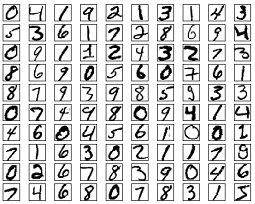
\includegraphics[width=.6\textwidth]{mnist_100_digits}
\end{center}

然后开发出一个可以从这些训练样本中进行学习的系统。换言之,神经网络使用样本来自动
推断出识别手写数字的规则。另外,通过增加训练样本的数量,网络可以学到更多关于手写
数字的知识,这样就能够提升自身的准确性。所以,上面例子中我们只是展出了 100 个训练
数字样本,而通过使用数千或者数百万或者数十亿的训练样本我们也许能够得到更好的手写
数字识别器。

本章我们将实现一个可以识别手写数字的神经网络。这个程序仅仅 74 行,不使用特别的神
经网络库。然而,这个短小的网络不需要人类帮助便可以超过 96\% 的准确率识别数字。而
且,在后面的章节,我们会发展出将准确率提升到 99\% 的技术。实际上,最优的商业神经
网络已经足够好到被银行和邮局分别用在账单核查和识别地址上了。

手写识别常常被当成学习神经网络的原型问题,因此我们聚焦在这个问题上。作为一个原型,
它具备一个关键点:挑战性~——~识别手写数字并不轻松~——~但也不会难到需要超级复杂的解
决方法,或者超大规模的计算资源。另外,这其实也是一种发展出诸如深度学习更加高级的
技术的方法。所以,整本书我们都会持续地讨论手写数字识别问题。本书后面部分,我们会
讨论这些想法如何用在其他计算机视觉的问题或者语音、自然语言处理和其他一些领域中。

当然,如果仅仅为了编写一个计算机程序来识别手写数字,本章的内容可以简短很多!但前
进的道路上,我们将扩展出很多关于神经网络的关键的思想,其中包括两个重要的人工神经
元(\gls*{perceptron}和S型神经元),以及标准的神经网络学习算法,即随机梯度下降算法。自始至
终,我专注于解释事情的原委,并构筑你对神经网络的直观感受。这需要一个漫长的讨论,
而不是仅仅介绍些基本的技巧,但这对于更深入的理解是值得的。作为收益,在本章的最后,
我们会准备好了解什么是深度学习,以及它为什么很重要。

\section{\gls*{perceptron}}
\label{sec:Perceptrons}

什么是神经网络?一开始,我将解释一种被称为\emph{\gls{perceptron}}\,的人工神经元。
\gls*{perceptron}在20世纪五、六十年代由科学家
\href{http://en.wikipedia.org/wiki/Frank_Rosenblatt}{Frank Rosenblatt}
\href{http://books.google.ca/books/about/Principles_of_neurodynamics.html?id=7FhRAAAAMAAJ}{%
  发明},其受到 \href{http://en.wikipedia.org/wiki/Warren_McCulloch}{Warren
  McCulloch} 和 \href{http://en.wikipedia.org/wiki/Walter_Pitts}{Walter Pitts}早
期\href{http://scholar.google.ca/scholar?cluster=4035975255085082870}{著作}的影
响。今天,使用其它人工神经元模型更为普遍~——~在这本书中,以及更多现代的神经网络著
作中,主要使用的是一种叫做\emph{\gls{sigmoid-neuron}}\,的神经元模型。我们很快会
讲到\gls*{sigmoid-neuron}。但是要理解为什么\gls*{sigmoid-neuron}被定义为那样的方
式,值得花点时间先来理解下\gls*{perceptron}。

\gls*{perceptron}是如何工作的呢?一个\gls*{perceptron}接受几个二进制输入,
$x_1,x_2,\ldots$,并产生一个二进制输出:
\begin{center}
  \includegraphics{tikz0}
\end{center}

示例中的\gls*{perceptron}有三个输入,$x_1,x_2,x_3$。通常可以有更多或更少输入。
Rosenblatt 提议一个简单的规则来计算输出。他引入\emph{\gls{weight}},
$w_1,w_2,\ldots$,表示相应输入对于输出重要性的实数。神经元的输出,$0$ 或者 $1$,
则由分配权重后的总和 $\sum_j w_j x_j$ 小于或者大于一些\emph{阈值}决定。和权重一
样,阈值是一个实数,一个神经元的参数。用更精确的代数形式:
\begin{equation}
  \text{output} = \begin{cases}
    0 & \quad \text{if } \sum_j w_j x_j \leq \text{ threshold} \\
    1 & \quad \text{if } \sum_j w_j x_j > \text{ threshold} \\
  \end{cases}
  \tag{1}
\end{equation}

这就是一个\gls*{perceptron}所要做的所有事情!

这是基本的数学模型。你可以将\gls*{perceptron}看作依据权重来作出决定的设备。让我
举个例子。这不是非常真实的例子,但是容易理解,而且很快我们会有根多实际的例子。假
设这个周末就要来了,你听说你所在的城市有个奶酪节。你喜欢奶酪,正试着决定是否去参
加。你也许会通过给三个因素设置权重来作出决定:
\begin{enumerate}
\item 天气好吗?
\item 你的男朋友或者女朋友会不会陪你去?
\item 这个节日举办的地点是否靠近交通站点?(你没有车)
\end{enumerate}

你可以把这三个因素对应地用二进制变量 $x_1,x_2$ 和 $x_3$ 来表示。例如,如果天气好,
我们把 $x_1 = 1$,如果不好,$x_1 = 0$。类似地,如果你的男朋友或女朋友同去,$x_2
= 1$,否则 $x_2 = 0$。$x_3$ 也类似地表示交通情况。

现在,假设你是个嗜好奶酪的吃货,以至于即使你的男朋友或女朋友不感兴趣,也不管路有
多难走都乐意去。但是也许你确实厌恶糟糕的天气,而且如果天气太糟你也没法出门。你可
以使用\gls*{perceptron}来给这种决策建立数学模型。一种方式是给天气权重选择为 $w_1
= 6$ ,其它条件为 $w_2 = 2$ 和 $w_3 = 2$。$w_1$ 被赋予更大的值,表示天气对你很重
要,比你的男朋友或女朋友陪你,或者最近的交通站重要的多。最后,假设你将%
\gls*{perceptron}的阈值设为 $5$。这样,\gls*{perceptron}实现了期望的决策模型,只
要天气好就输出 $1$,天气不好则为 $0$。对于你的男朋友或女朋友是否想去,或者附近是
否有公共交通站,其输出则没有差别。

随着权重和阈值的变化,你可以得到不同的决策模型。例如,假设我们把阈值改为 $3$ 。
那么\gls*{perceptron}会按照天气好坏,或者结合交通情况和你男朋友或女朋友同行的意愿,来得出结
果。换句话说,它变成了另一个不同的决策模型。降低阈值则表示你更愿意去。

很明显,\gls*{perceptron}不是人做出决策使用的全部模型。但是这个例子说明了一个\gls*{perceptron}如何能权
衡不同的依据来决策。这看上去也可以大致解释一个\gls*{perceptron}网络能够做出微妙的决定:
\begin{center}
  \includegraphics{tikz1}
\end{center}

在这个网络中,第一列\gls*{perceptron}~——~我们称其为第一层\gls*{perceptron}~——~通过权衡输入依据做出三个
非常简单的决定。那第二层的\gls*{perceptron}呢?每一个都在权衡第一层的决策结果并做出决定。以
这种方式,一个第二层中的\gls*{perceptron}可以比第一层中的做出更复杂和抽象的决策。在第三层中
的\gls*{perceptron}甚至能进行更复杂的决策。以这种方式,一个多层的\gls*{perceptron}网络可以从事复杂巧妙
的决策。

顺便提一下,当我定义\gls*{perceptron}时我说的是\gls*{perceptron}只有一个输出。在上面的网络中\gls*{perceptron}看上
去像是有多个输出。实际上,他们仍然是单输出的。多个\gls*{perceptron}输出箭头仅仅便于说明一个
\gls*{perceptron}的输出被用于其它\gls*{perceptron}的输入。它和把单个输出线条分叉相比,显得讨巧些。

让我们简化\gls*{perceptron}的数学描述。条件 $\sum_j w_j x_j$ 看上去有些冗长,我们可以创建两
个符号的变动来简化。第一个变动是把 $\sum_j w_j x_j$ 改写成点乘,$w \cdot x
\equiv \sum_j w_j x_j$,这里 $w$ 和 $x$ 对应权重和输入的向量。第二个变动是把阈值
移到不等式的另一边,并用\gls*{perceptron}的偏置\index{偏置} $b \equiv -threshold$ 代替。用偏置而
不是阈值,那么\gls*{perceptron}的规则可以重写为:
\begin{equation}
  \text{output} = \begin{cases}
    0 & \quad \text{if } w\cdot x + b \leq 0 \\
    1 & \quad \text{if } w\cdot x + b > 0
  \end{cases}
  \tag{2}
\end{equation}

我们可以把偏置看作一种表示让\gls*{perceptron}输出 $1$(或者用生物学的术语,即激活\gls*{perceptron})有
多容易的估算。对于具有一个非常大偏置的\gls*{perceptron}来说,输出 $1$ 是很容易的。但是如果偏
置是一个非常小的负数,输出 $1$ 则很困难。很明显,引入偏置只是我们描述\gls*{perceptron}的一个
很小的变动,但是我们后面会看到它引导更进一步的符号简化。因此,在这本书的后续部分,
我们不再用阈值,而总是使用偏置。

我已经描述过\gls*{perceptron}是一种权衡依据来做出决策的方法。\gls*{perceptron}被采用的另一种方式,是计
算基本的逻辑功能,即我们通常认为的运算基础,例
如“\emph{与}”,“\emph{或}”和“\emph{与非}”。例如,假设我们有个两个输入的感知
器,每个权重为 $-2$,整体的偏置为 $3$。这是我们的\gls*{perceptron}:
\begin{center}
  \includegraphics{tikz2}
\end{center}

这样我们得到:输入 $00$ 产生输出 $1$,即 $(-2)*0 + (-2)*0 + 3 = 3$ 是正数。这里
我用 $*$ 符号来显式地表示乘法。但是输入 $11$ 产生输出 $0$,即 $(-2)*1 + (-2)*1
+ 3 = -1$ 是负数。如此我们的\gls*{perceptron}实现了一个与非门!

与非门的例子显示了我们可以用\gls*{perceptron}来计算简单的逻辑功能。实际上,我们完全能用感知
器网络来计算任何逻辑功能。原因是与非门是通用运算,那样,我们能在多个与非门之上构
建出任何运算。例如,我们能用与非门构建一个电路,它把两个二进制数 $x_1$ 和 $x_2$
相加。这需要计算按位求和,$x_1 \oplus x_2$,同时当 $x_1$ 和 $x_2$ 都为 $1$ 时进
位设为 $1$,即进位位正好是按位乘积 $x_1x_2$:
\begin{center}
  \includegraphics{tikz3}
\end{center}

为了得到相等的\gls*{perceptron}网络,我们把所有与非门替换为\gls*{perceptron},其具有两个输入、每个权重
设为 $-2$,整体偏置为 $3$。结果我们得到这样的网络。注意我已经把右下的与非门移动了
一点,只是为了在图上更方便画箭头:
\begin{center}
  \includegraphics{tikz4}
\end{center}

这个\gls*{perceptron}网络中有一个部分值得注意,最左边的\gls*{perceptron}的输出被两次作为底部\gls*{perceptron}的输
入。当我定义\gls*{perceptron}模型时,我没有说过是否允许这种双输出到同一个地方。实际上这不重
要。如果我们不想允许这种形式,那可以简单把两条线合并为到一个权重为 $-4$ 的连接,
而不是两个权重为 $-2$ 的连接。(如果你还没明白,应该停下来证明这是相等的。)随着
这一改变,原先的网络看起来像下面描绘的,所有未标记的权重等于 $-2$,所有偏置等于
$3$,标记的单个权重为 $-4$:
\begin{center}
  \includegraphics{tikz5}
\end{center}

目前为止我把像 $x_1$ 和 $x_2$ 这样的输入画成\gls*{perceptron}网络左边浮动的变量。实际上,可
以画一层额外的\gls*{perceptron}~——~输入层~——~来方便对输入编码:
\begin{center}
  \includegraphics{tikz6}
\end{center}

这种对有一个输出但没有输入的\gls*{perceptron}的标记法,
\begin{center}
  \includegraphics{tikz7}
\end{center}
是一种标准。它并不实际表示一个\gls*{perceptron}没有输入。为了看清它,假设我们确实有一个没有
输入的\gls*{perceptron}。那么加权和 $\sum_j w_j x_j$ 会总是为零,并且\gls*{perceptron}在 $b > 0$ 时输
出 $1$,当 $b \leq 0$时输出 $0$。那样,\gls*{perceptron}会简单输出一个固定值,而不是期望值
(上例中的 $x_1$)。倒不如完全不把输入\gls*{perceptron}看作\gls*{perceptron},而是简单定义为输出期望值
的特殊单元,$x_1, x_2,\ldots$。

这个加法器的例子演示了一个\gls*{perceptron}网络如何用于模拟包含很多与非门的电路。因为与非门
在计算机运算中的通用性,由此可以得出\gls*{perceptron}也同样适用的结论。

\gls*{perceptron}运算的通用性既是令人鼓舞的,又是令人失望的。令人鼓舞是因为它告诉我们\gls*{perceptron}
网络能和其它计算设备一样强大。但是它也令人失望,因为它看上去只不过是一种新的与非
门。这简直不算个大新闻!

然而,实际情况比这一观点认为的更好。其结果是我们可以设计\emph{学习算法},能够自
动调整人工神经元的权重和偏置。这种调整可以响应外部的刺激,而不需要一个程序员的直
接干预。这些学习算法是我们能够以一种根本区别于传统逻辑门的方式使用人工神经元。有
别于显式地设计\emph{与非}或其它门,我们的神经网络能简单地学会解决问题,这些问题
有时候直接用传统的电路设计是很难解决的。

\section{S型神经元}
\label{seq:sigmoid_neurons}

学习算法听上去非常棒。但是我们怎样给一个神经网络设计这样的算法呢?假设我们有一个
\gls*{perceptron}网络,想要用它来解决一些问题。例如,网络的输入可以是一幅手写数字的扫描图像。
我们想要网络能学习权重和偏置,这样网络的输出能正确分类这些数字。为了看清学习是怎
样工作的,假设我们把网络中的权重(或者偏置)做些微小的改动。就像我们马上会看到的,
这一属性会让学习变得可能。这里简要示意我们想要的(很明显这个网络对于手写识别还是
  太简单了!):
\begin{center}
  \includegraphics{tikz8}  
\end{center}

如果对权重(或者偏置)的微小的改动真的能够仅仅引起输出的微小变化,那我们可以利用
这一事实来修改权重和偏置,让我们的网络能够表现得像我们想要的那样。例如,假设网络
错误地把一个“9”的图像分类为“8”。我们能够计算出怎么对权重和偏置做些小的改动,
这样网络能够接近于把图像分类为“9”。然后我们要重复这个工作,反复改动权重和偏置
来产生更好的输出。这时网络就在学习。

问题在于当我们的网络包含\gls*{perceptron}时这不会发生。实际上,网络中单个\gls*{perceptron}上一个权重或
偏置的微小改动有时候会引起那个\gls*{perceptron}的输出完全翻转,如 $0$ 变到$1$。那样的翻转可
能接下来引起其余网络的行为以极其复杂的方式完全改变。因此,虽然你的“9”可能被正
确分类,网络在其它图像上的行为很可能以一些很难控制的方式被完全改变。这使得逐步修
改权重和偏置来让网络接近期望行为变得困难。也许有其它聪明的方式来解决这个问题。但
是这不是显而易见地能让一个\gls*{perceptron}网络去学习。

我们可以引入一种称为S型神经元的新的人工神经元来克服这个问题。S型神经元和\gls*{perceptron}类
似,但是被修改为权重和偏置的微小改动只引起输出的微小变化。这对于让神经元网络学习
起来是很关键的。

好了, 让我来描述下S型神经元。我们用描绘\gls*{perceptron}的相同方式来描绘
S型神经元\index{S型神经元}:
\begin{center}
  \includegraphics{tikz9}
\end{center}

正如一个\gls*{perceptron},S型神经元有多个输入,$x_1,x_2,\ldots$。但是这些输入可以取 $0$ 和
$1$ 中的任意值,而不仅仅是 $0$ 或 $1$。例如,$0.638\ldots$ 是一个S型神经元的有效
输入。同样,S型神经元对每个输入有权重,$w_1,w_2,\ldots$,和一个总的偏置,$b$。但
是输出不是 $0$ 或 $1$。相反,它现在是 $\sigma(w \cdot x+b)$,这里 $\sigma$ 被称
为S型函数\footnote{顺便提一下,$\sigma$ 有时被称为\emph{逻辑函数},而这种新的神
  经元类型被称为\emph{逻辑神经元}。既然这些术语被很多从事于神经元网络的人使用,
  记住它是有用的。然而,我们将继续使用S型这个术语。},定义为:
\begin{equation}
  \sigma(z) \equiv \frac{1}{1+e^{-z}}
  \label{eq:3}\tag{3}
\end{equation}

把它们放在一起来更清楚地说明,一个具有输入 $x_1,x_2,\ldots$,权重
$w_1,w_2,\ldots$,和偏置 $b$ 的S型神经元的输出是:
\begin{equation}
  \frac{1}{1+\exp(-\sum_j w_j x_j-b)}
  \label{eq:4}\tag{4}
\end{equation}

初看上去,S型神经元和\gls*{perceptron}有很大的差别。如果你不熟悉S型函数的代数形式,它看上去
晦涩难懂又令人生畏。实际上,\gls*{perceptron}和S型神经元之间有很多相似的地方,跨过理解上的
障碍,S型函数的代数形式具有很多技术细节。

为了理解和\gls*{perceptron}模型的相似性,假设 $z \equiv w \cdot x + b$ 是一个很大的正数。那
么 $e^{-z} \approx 0$ 而 $\sigma(z) \approx 1$。即,当 $z = w \cdot x+b$ 很大
并且为正,S型神经元的输出近似为 $1$,正好和\gls*{perceptron}一样。相反地,假设 $z = w \cdot
x+b$ 是一个很大的负数。那么 $e^{-z} \rightarrow \infty$,$\sigma(z) \approx 0$。
所以当 $z = w \cdot x +b$ 是一个很大的负数,S型神经元的行为也非常近似一个\gls*{perceptron}。
只有在 $w \cdot x+b$ 取中间值时,和\gls*{perceptron}模型有比较大的偏离。

$\sigma$ 的代数形式又是什么?我们怎样去理解它呢?实际上,$\sigma$ 的精确形式不重
要~——~重要的是这个函数绘制的形状。是这样:
\begin{center}
  \includegraphics{sigmoid_function}
  \label{fig:SigmoidFunction}
\end{center}

这个形状是阶跃函数平滑后的版本:
\begin{center}
  \includegraphics{step_function}
  \label{fig:StepFunction}
\end{center}

如果 $\sigma$ 实际是个阶跃函数,既然输出会依赖于 $w\cdot x+b$ 是正数还是负
数\footnote{实际上,当 $w \cdot x +b = 0$ ,\gls*{perceptron}输出 $0$,而同时阶跃函数输出
  $1$。所以严格地说,我们需要修改阶跃函数来符合这点。但是你知道怎么做。},那么S
型神经元会成为一个\gls*{perceptron}。利用实际的 $\sigma$ 函数,我们得到一个,就像上面说明的,
平滑的\gls*{perceptron}。的确,$\sigma$ 函数的平滑特性,正是关键因素,而不是其细部形式。
$\sigma$ 的平滑意味着权重和偏置的微小变化,即 $\Delta w_j$ 和 $\Delta b$,会从神
经元产生一个微小的输出变化 $\Delta \mbox{output}$。实际上,微积分告诉我们
$\Delta \mbox{output}$ 可以很好地近似表示为:
\begin{equation}
  \Delta \mbox{output} \approx \sum_j \frac{\partial \, \mbox{output}}{\partial w_j}
  \Delta w_j + \frac{\partial \, \mbox{output}}{\partial b} \Delta b
  \label{eq:5}\tag{5}
\end{equation}

其中求和是在所有权重 $w_j$ 上进行的,而 $\partial \, \mbox{output} / \partial w_j$ 和
$\partial \, \mbox{output} /\partial b$ 符号表示 $output$ 分别对于 $w_j$和 $b$
的偏导数。如果你对偏导数感到不自在,不用惊慌。上面全部用偏导数的表达式看上去很复
杂,实际上它的意思非常简单(这可是个好消息):$\Delta \mbox{output}$ 是一个反映
权重和偏置变化~——~即 $\Delta w_j$ 和 $\Delta b$~——~的线性函数。这一线性使得选择
权重和偏置的微小变化来达到输出的微小变化的运算变得容易。所以当S型神经元有更多和
\gls*{perceptron}相同的本质的行为时,计算如何变化权重和偏置来使输出变化会更加容易。

如果对 $\sigma$ 来说重要的是形状而不是精确的形式,那为什么要在公式~\eqref{eq:3}
中给 $\sigma$ 使用特定的形式呢?实际上,在这本书的后面我们会碰巧考虑到为其它激活
函数 $f(\cdot)$ 输出为 $f(w \cdot x + b)$ 的神经元。当我们使用一个不同的激活函数,
最大的变化是公式~\eqref{eq:5} 中用于偏导数的特定值的改变。事实证明当我们后面计算
这些偏导数,用 $\sigma$ 会简化数学计算,这是因为指数在求导时有些可爱的属性。无论
如何,$\sigma$ 在神经网络的工作中被普遍使用,并且是这本书中我们最常使用的激活函
数。

我们应该如何解释一个S型神经元的输出呢?很明显,\gls*{perceptron}和S型神经元之间一个很大的不
同是S型神经元不仅仅输出 $0$ 或 $1$。它可以输出 $0$ 和 $1$ 之间的任何实数,所以诸
如 $0.173\ldots$ 和 $0.689\ldots$ 的值是合理的输出。这是非常有用的,例如,当我们
想要输出来表示一个神经网络的图像像素输入的平均强度。但有时候这会是个麻烦。假设我
们希望网络的输出表示“输入图像是一个9”或“输入图像不是一个9”。很明显,如果输出
是 $0$ 或 $1$ 是最简单的,就像用\gls*{perceptron}。但是在实践中,我们可以设定一个约定来解决
这个问题,例如,约定任何至少为 $0.5$ 的输出为表示 “这是一个9”,而其它小于
$0.5$ 的输出为表示 “不是一个9”。当我们正在使用这样的约定时,我总会清楚地提出来,
这样就不会引起混淆。

\subsection*{练习}

\begin{itemize}
\item \textbf{S型神经元模拟\gls*{perceptron},第一部分}\\假设我们把一个\gls*{perceptron}网络中的所有权
  重和偏置乘以一个正的常数,$c>0$。证明网络的行为并没有改变。
\item \textbf{S型神经元模拟\gls*{perceptron},第二部分}\\假设我们有上题中相同的设置~——~一个
  \gls*{perceptron}网络。同样假设所有输入被选中。我们不需要实际的输入值,仅仅需要固定这些输
  入。假设对于网络中任何特定\gls*{perceptron}的输入 $x$, 权重和偏置遵循 $w \cdot x + b
  \neq 0$。现在用S型神经元替换所有网络中的\gls*{perceptron},并且把权重和偏置乘以一个正的常
  量$c>0$。证明在$c \rightarrow \infty$的极限情况下,S型神经元网络的行为和\gls*{perceptron}
  网络的完全一致。当一个\gls*{perceptron}的 $w \cdot x + b = 0$ 时又为什么会不同?
\end{itemize}

\section{神经网络的架构}

在下一节我会介绍一个神经网络,我们可以用它来很好地分类手写数字。准备进入下一节时,
解释一些可以让我们命名网络中不同部分的术语是很有帮助的。假设我们有这样的网络:
\begin{center}
  \includegraphics{tikz10}
\end{center}

前面提过,这个网络中最左边的称为输入层,其中的神经元称为\emph{输入神经元}\index{输入神经元}。
最右边的,即\emph{输出}层包含有\emph{输出神经元}\index{输出神经元},在本例中,输出层只有一个神经元。
中间层,既然这层中的神经元既不是输入也不是输出,则被称为\emph{隐藏层}\index{隐藏层}。
“隐藏”这一术语也许听上去有些神秘~——~我第一次听到这个词,以为它必然有一些深层的哲学或数学涵意~——~
但它实际上仅仅意味着“既非输入也非输出”。上面的网络仅有一个隐藏层,但有些网络有多个隐藏层。例如,
下面的四层网络有两个隐藏层:
\begin{center}
  \includegraphics{tikz11}
\end{center}

有些令人困惑的是,由于历史的原因,尽管是由S型神经元而不是\gls*{perceptron}构成,这种多层网
络有时被称为\emph{多层\gls*{perceptron}}\index{多层\gls*{perceptron}}或者\emph{MLP}\index{MLP}。在这本书中我不会使用 MLP 这个术语,因为我
认为这会引起混淆,但这里想提醒你它的存在。

设计网络的输入输出层通常是比较直接的。例如,假设我们尝试确定一张手写数字的图像上
是否写的是“9”。很自然地,我们可以将图片像素的强度进行编码作为输入神经元来设计
网络。如果图像是一个 $64 \times 64$ 的灰度图像,那么我们会需要 $4096 = 64 \times
64$ 个输入神经元,每个强度取 $0$ 和 $1$ 之间合适的值。输出层只需要包含一个神经元,
当输出值小于 $0.5$ 时表示 “输入图像不是一个 $9$”,大于 $0.5$ 的值表示 “输入图
像是一个 $9$”。

相比于神经网络中输入输出层的直观设计,隐藏层的设计则堪称一门艺术。特别是,通过一
些简单的经验法则来总结隐藏层的设计流程是不可行的。相反,神经网络的研究人员已经为
隐藏层开发了许多设计最优法则,这有助于网络的行为能符合人们期望的那样。例如,这些
法则可以用于帮助权衡隐藏层数量和训练网络所需的时间开销。在本书后面我们会碰到几个
这样的设计最优法则。

目前为止,我们讨论的神经网络,都是以上一层的输出作为下一层的输入。这种网络被称为
\emph{前馈}神经网络\index{前馈神经网络}。这意味着网络中是没有回路的~——~信息总是向前传播,从不反向回
馈。如果确实有回路,我们最终会有这样的情况:$\sigma$ 函数的输入依赖于输出。这将
难于理解,所以我们不允许这样的环路。

然而,也有一些人工神经网络的模型,其中反馈环路是可行的。这些模型被称为%
\href{http://en.wikipedia.org/wiki/Recurrent_neural_network}{递归神经网络}\index{递归神经网络}。这种
模型的设计思想,是具有休眠前会在一段有限的时间内保持激活状态的神经元。这种激活状
态可以刺激其它神经元,使其随后被激活并同样保持一段有限的时间。这样会导致更多的神
经元被激活,随着时间的推移,我们得到一个级联的神经元激活系统。因为一个神经元的输
出只在一段时间后而不是即刻影响它的输入,在这个模型中回路并不会引起问题。

递归神经网络比前馈网络影响力小得多,部分原因是递归网络的学习算法(至少目前为止)
不够强大。但是递归网络仍然很有吸引力。它们原理上比前馈网络更接近我们大脑的实际工
作。并且递归网络能解决一些重要的问题,这些问题如果仅仅用前馈网络来解决,则更加困
难。然而为了篇幅,本书将专注于使用更广泛的前馈网络。

\section{一个简单的分类手写数字的网络}

定义神经网络后,让我们回到手写识别上来。我们可以把识别手写数字的问题分成两个子问
题。首先,我们希望有个方式把包含许多数字的图像分成一系列单独的图像,每个包含单个
数字。例如,我们想要把图像
\begin{center}
  
\includegraphics[width=64pt]{digits}
\end{center}
分成六个单独的图像,
\begin{center}
  
\includegraphics[height=32pt]{digits_separate}
\end{center}

我们人类可以很容易解决这个分割的问题,但是对于计算机程序来说却是个挑战。一旦图像
被分割,那么程序需要把每个单独的数字分类。例如,我们想要我们的程序能识别上面的第
一个数字
\begin{center}
  
\includegraphics[height=24pt]{mnist_first_digit}
\end{center}
是 $5$。

我们将专注于编程解决第二个问题,分类单独的数字。这样是因为,一旦你有分类单独数字
的有效方法,分割问题是不难解决的。有很多途径可以解决分割的问题。一种方法是尝试不
同的分割方式,用数字分类器对每一个切分片段打分。如果数字分类器对每一个片段的置信
度都比较高,那么这个分割方式就能得到较高的分数;如果数字分类器在一或多个片段中出
现问题,那么这种分割方式就会得到较低的分数。这种方法的思想是,如果分类器有问题,
那么很可能是由于图像分割出错导致的。这种思想以及它的变化形式能够比较好地解决分割
问题。因此,与其关心分割问题,我们不如把精力集中在设计一个神经网络来解决更有趣、
更困难的问题,即手写数字的识别。

我们将使用一个三层神经网络来识别单个数字:
\begin{center}
  \includegraphics{tikz12}
\end{center}

网络的输入层包含给输入像素的值进行编码的神经元。就像下一节会讨论的,我们给网络的
训练数据会有很多扫描得到的 $28 \times 28$ 的手写数字的图像组成,所有输入层包含有
$784 = 28 \times 28$ 个神经元。为了简化,上图中我已经忽略了 $784$ 中大部分的输入
神经元。输入像素是灰度级的,值为 $0.0$ 表示白色,值为 $1.0$ 表示黑色,中间数值表
示逐渐暗淡的灰色。

网络的第二层是一个隐藏层。我们用 $n$ 来表示神经元的数量,我们将给 $n$ 实验不同的
数值。示例中用一个小的隐藏层来说明,仅仅包含 $n=15$ 个神经元。

网络的输出层包含有 $10$ 个神经元。如果第一个神经元激活,即输出 $\approx 1$,那么
表明网络认为数字是一个 $0$。如果第二个神经元激活,就表明网络认为数字是一个 $1$。
依此类推。更确切地说,我们把输出神经元的输出赋予编号 $0$ 到 $9$,并计算出那个神
经元有最高的激活值。比如,如果编号为 $6$ 的神经元激活,那么我们的网络会猜到输入
的数字是 $6$。其它神经元相同。

你可能会好奇为什么我们用 $10$ 个输出神经元。毕竟我们的任务是能让神经网络告诉我们
哪个数字( $0, 1, 2, \ldots, 9$ )能和输入图片匹配。一个看起来更自然的方式就是使
用 $4$ 个输出神经元,把每一个当做一个二进制值,结果取决于它的输出更靠近 $0$ 还是
$1$~。四个神经元足够编码这个问题了,因为 $2^4 = 16$ 大于 $10$ 种可能的输入。为什
么我们反而要用 $10$ 个神经元呢?这样做难道效率不低吗?最终的判断是基于经验主义的:
我们可以实验两种不同的网络设计,结果证明对于这个特定的问题而言,$10$ 个输出神经
元的神经网络比4个的识别效果更好。但是令我们好奇的是为什么使用 $10$ 个输出神经元
的神经网络更有效呢。有没有什么启发性的方法能提前告诉我们用10个输出编码比使用 $4$
个输出编码更有好呢?

为了理解为什么我们这么做,我们需要从根本原理上理解神经网络究竟在做些什么。首先考
虑有 $10$ 个神经元的情况。我们首先考虑第一个输出神经元,它告诉我们一个数字是不是
0。它能那么做是因为可以权衡从隐藏层来的信息。隐藏层的神经元在做什么呢?假设隐藏
层的第一个神经元只是用于检测如下的图像是否存在:
\begin{center}
  
\includegraphics[height=32pt]{mnist_top_left_feature}
\end{center}

为了达到这个目的,它通过对此图像对应部分的像素赋予较大权重,对其它部分赋予较小的
权重。同理,我们可以假设隐藏层的第二,第三,第四个神经元是为检测下列图片是否存在:
\begin{center}
  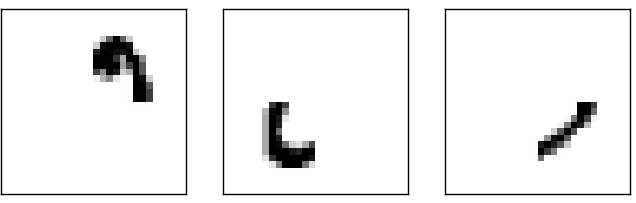
\includegraphics[height=32pt]{mnist_other_features}
\end{center}

就像你能猜到的,这四幅图像组合在一起构成了\hyperref[fig:digits]{前面}显示的一行
数字图像中的 $0$:
\begin{center}
  
\includegraphics[height=32pt]{mnist_complete_zero}
\end{center}

如果所有隐藏层的这四个神经元被激活那么我们就可以推断出这个数字是 $0$。当然,这不
是我们推断出 $0$ 的唯一方式~——~我们能通过很多其他合理的方式得到 $0$ (举个例子来说,
  通过上述图像的转换,或者稍微变形)。但至少在这个例子中我们可以推断出输入的数字
是 $0$。

假设神经网络以上述方式运行,我们可以给出一个貌似合理的理由去解释为什么用 $10$ 个
输出而不是 $4$ 个。如果我们有 $4$ 个输出,那么第一个输出神经元将会尽力去判断数字
的最高有效位是什么。把数字的最高有效位和数字的形状联系起来并不是一个简单的问题。
很难想象出有什么恰当的历史原因,一个数字的形状要素会和一个数字的最高有效位有什么
紧密联系。

上面我们说的只是一个启发性的方法。没有什么理由表明这个三层的神经网络必须按照我所
描述的方式运行,即隐藏层是用来探测数字的组成形状。可能一个聪明的学习算法将会找到
一些合适的权重能让我们仅仅用4个输出神经元就行。但是这个启发性的方法通常很有效,
它会节省你大量时间去设计一个好的神经网络结构。

\subsection*{练习}

\begin{itemize}
\item 通过在上述的三层神经网络加一个额外的一层就可以实现按位表示数字。额外的一层
  把原来的输出层转化为一个二进制表示,如下图所示。为新的输出层寻找一些合适的权重
  和偏置。假定原先的3层神经网络在第三层得到正确输出(即原来的输出层)的激活值至
  少是 $0.99$,得到错误的输出的激活值至多是 $0.01$。
  \begin{center}
    \includegraphics{tikz13}
  \end{center}
\end{itemize}

\section{使用梯度下降算法进行学习}
\label{sec:learning_with_gradient_descent}

现在我们有了神经网络的设计,它怎样可以学习识别数字呢?我们需要的第一样东西是一个
用来学习的数据集~——~称为训练数据集。我们将使用
\href{http://yann.lecun.com/exdb/mnist/}{MNIST 数据集},其包含有数以万计的连带着
正确分类器的手写数字的扫描图像。MNIST的名字来源于
\href{http://en.wikipedia.org/wiki/National_Institute_of_Standards_and_Technology}{NIST}
—— 美国国家标准与技术研究所~——~收集的两个数据集改进后的子集。这是取自 MNIST 的一
些图像:
\begin{center}
  
\includegraphics[height=32pt]{digits_separate}
\end{center}

正如你看到的,这些数字其实是和本章\hyperref[fig:digits]{开始}提到的一样。当然,
当测试我们的网络时我们将要求它识别不在训练集中的图像。

MNIST 数据分为两个部分。第一部分包含 60,000 幅用于训练数据的图像。这些图像扫描自
250 人的手写样本,他们中一半人是美国人口普查局的员工,一半人是高校学生。这些图像
是 $28 \times 28$ 大小的灰度图像。第二部分是 10,000 幅用于测试数据的图像,同样是
$28 \times 28$ 的灰度图像。我们将用这些测试数据来评估我们的神经网络学会识别数字
有多好。为了让其有好的测试表现,测试数据取自和原始训练数据不同的\emph{另外}一
组 250 人(尽管仍然分别是美国人口普查局和高校学生)。这有助于确保我们的系统能识
别那些没有看到训练数据的人写的数字。

我们将用符号 $x$ 来表示一个训练输入。为了方便,把每个训练输入 $x$ 看作一个 $28
\times 28 = 784$ 维的向量。每个向量中的项目代表图像中单个像素的灰度值。我们用 $y
= y(x)$ 表示对应的期望输出,这里 $y$ 是一个 $10$ 维的向量。例如,如果有一个特定
的画成 $6$ 的训练图像,$x$,那么 $y(x) = (0, 0, 0, 0, 0, 0, 1, 0, 0, 0)^T$ 则是
网络的期望输出。注意这里 $T$ 是转置操作,把一个行向量转换成一个列向量。

我们希望有一个算法,能让我们找到权重和偏置,以至于网络的输出 $y(x)$ 能够拟合所有
的训练输入$x$。为了量化我们如何实现这个目标,我们定义一个\emph{代价函
  数}\index{代价函数}\footnote{有时被称为\emph{损失}或\emph{目标}函数。我们在这
  本书中使用了代价函数这个术语,但是你应该注意其他的术语,因为它经常被用于研究论
  文和其他神经网络的讨论中。}:
\begin{equation}
  C(w,b) \equiv \frac{1}{2n} \sum_x \| y(x) - a\|^2
  \label{eq:6}\tag{6}
\end{equation}

这里 $w$ 表示所有的网络中权重的集合,$b$ 是所有的偏置,$n$ 是训练输入数据的个数,
$a$ 是表示当输入为 $x$ 时输出的向量,求和则是在总的训练输入 $x$ 上进行的。当然,
输出 $a$ 取决于 $x$, $w$ 和 $b$,但是为了保持符号的简洁性,我没有明确地指出这种
依赖关系。符号 $\|v\|$ 是指向量 $v$ 的模。我们把 $C$ 称为\emph{二次}代价函数\index{二次代价函数};有
时也被称为\emph{均方误差}\index{均方误差}或者\emph{MSE}\index{MSE}。观察二次代价函数的形式我们可以看到
$C(w,b)$ 是非负的,因为求和公式中的每一项都是非负的。此外,代价函数 $C(w,b)$的值
相当小,即 $C(w,b) \approx 0$,精确地说,是当对于所有的训练输入 $x$,$y(x)$接近
于输出 $a$ 时。因此如果我们的学习算法能找到合适的权重和偏置,使得 $C(w,b)
\approx 0$,它就能很好地工作。相反,当 $C(w,b)$ 很大时就不怎么好了,那意味着对于
大量地输入, $y(x)$ 与输出 $a$ 相差很大。因此我们的训练算法的目的,是最小化权重
和偏置的代价函数 $C(w,b)$。换句话说,我们想要找到一系列能让代价尽可能小的权重和
偏置。我们将采用称为\emph{梯度下降}\index{梯度下降}的算法来达到这个目的。

为什么要介绍二次代价呢?毕竟我们最初感兴趣的内容不是能正确分类的图像数量吗?为什
么不试着直接最大化这个数量,而是去最小化一个类似二次代价的间接评量呢?这么做是因
为在神经网络中,被正确分类的图像数量所关于权重和偏置的函数并不是一个平滑的函数。
大多数情况下,对权重和偏置做出的微小变动完全不会影响被正确分类的图像的数量。这会
导致我们很难去解决如何改变权重和偏置来取得改进的性能。而用一个类似二次代价的平滑
代价函数则能更好地去解决如何用权重和偏置中的微小的改变来取得更好的效果。这就是为
什么我们首先专注于最小化二次代价,只有这样,我们之后才能测试分类精度。

即使已经知道我们需要使用一个平滑的代价函数,你可能仍然想知道为什么我们在方
程~\eqref{eq:6} 中选择二次函数。这是\emph{临时}想出来的吗?是不是我们选择另一个不同的代
价函数将会得到完全不同的最小化的权重和偏置呢?这种顾虑是合理的,我们后面会再次回
到这个代价函数,并做一些修改。尽管如此,方程~\eqref{eq:6} 中的二次代价函数让我们
更好地理解神经网络中学习算法的基础,所以目前我们会一直使用它。

重复一下,我们训练神经网络的目的是找到能最小化二次代价函数 $C(w,b)$ 的权重和偏置。
这是一个适定问题,但是现在它有很多让我们分散精力的结构~——~对权重 $w$ 和偏置 $b$
的解释,晦涩不清的 $\sigma$ 函数,神经网络结构的选择,MNIST 等等。事实证明我们可
以忽略结构中大部分,把精力集中在最小化方面来理解它。现在我们打算忘掉所有关于代价
函数的具体形式、神经网络的连接等等。现在让我们想象只要最小化一个给定的多元函数。
我们打算使用一种被称为\emph{梯度下降}的技术来解决这样的最小化问题。然后我们回到
在神经网络中要最小化的特定函数上来。

好了,假设我们要最小化某些函数,$C(v)$。它可以是任意的多元实值函数,$v = v_1,
v_2, \ldots$。注意我们用 $v$ 代替了 $w$ 和 $b$ 以强调它可能是任意的函数~——~我们
现在先不局限于神经网络的环境。为了最小化 $C(v)$,想象 $C$ 是一个只有两个变量
$v1$和 $v2$ 的函数:
\begin{center}
  \includegraphics{valley}
\end{center}

我们想要的是找到 $C$ 的全局最小值。当然,对于上图的函数,我们一眼就能找到最小值。
那只意味着,也许我展示的函数\emph{过于}简单了!通常函数 $C$ 可能是一个复杂的多元
函数,看一下就能找到最小值是不可能的。

一种解决这个问题的方式是用微积分来解析最小值。我们可以计算导数去寻找 $C$ 的极值
点。运气好的话,$C$ 是一个只有一个或少数几个变量的函数。但是变量过多的话那就是噩
梦。而且神经网络中我们经常需要\emph{大量}的变量——最大的神经网络有依赖数亿权重和
偏置的代价函数,极其复杂。用微积分来计算最小值已经不可行了。

(确定我们将可以通过有两个变量的函数 $C$ 来理解神经网络后,我已经两次提到:“嘿,
  如果函数有远多于两个变量怎么办?”。对此我只能说很抱歉。请相信我把 $C$ 想象成
  一个二元函数是有助于我们的理解的。有时候这种想象的画面会遇到障碍,这正是上面两
  个段落在帮助你克服的。善于思考数学通常也涉及到有效地利用多种直觉上的想象画面,
  学会什么时候用什么画面合适。)

好吧,微积分是不能用了。幸运的是,有一个漂亮的推导法暗示有一种算法能得到很好的效
果。首先把我们的函数想象成一个山谷。只要瞄一眼上面的绘图就不难理解。我们想象有一
个小球从山谷的斜坡滚落下来。我们的日常经验告诉我们这个球最终会滚到谷底。也许我们
可以用这一想法来找到函数的最小值?我们会为一个(假想的)球体随机选择一个起始位置,
然后模拟球体滚落到谷底的运动。我们可以通过计算 $C$ 的导数(或者二阶导数)来简单
模拟——这些导数会告诉我们山谷中局部“形状”的一切,由此知道我们的球将怎样滚动。

看到这里你可能会以为我们会写下球体的牛顿运动定理,考虑摩擦力、重力等影响。实际上,
我们不打算真的去实现这个球体滚落的推导~——~我们是在设计一个最小化 $C$ 的算法,而
不是在用物理定律做精确的仿真。对球体的肉眼观察是为了激发我们的想象而不是束缚我们
的思维。因此与其陷进物理学里凌乱的细节,不如我们就这样问自己:如果我们扮演一天的
上帝,能够构造自己的物理定律,能够支配球体可以如何滚动,那么我们将会采取什么样的
运动学定律来让球体能够总是滚落到谷底呢?

为了更精确地描述这个问题,让我们思考一下,当我们在 $v1$ 和 $v2$ 方向分别将球体移
动一个很小的量,即 $\Delta v1$ 和 $\Delta v2$ 时,球体将会发生什么情况。微积分告
诉我们 $C$ 将会有如下变化:
\begin{equation}
  \Delta C \approx \frac{\partial C}{\partial v_1} \Delta v_1 +
  \frac{\partial C}{\partial v_2} \Delta v_2
  \label{eq:7}\tag{7}
\end{equation}

我们要寻找一种选择 $\Delta v_1$ 和 $\Delta v_2$ 的方法使得 $\Delta C$ 为负;即,
我们选择它们是为了让球体滚落。为了弄明白如何选择,需要定义 $\Delta v$ 为 $v$ 变
化的向量,$\Delta v \equiv (\Delta v_1, \Delta v_2)^T$,$T$ 是转置符号。我们也定
义 $C$ 的梯度为偏导数的向量,$\left(\frac{\partial C}{\partial v_1},
\frac{\partial C}{\partial v_2}\right)^T$。我们用 $\nabla C$ 来表示梯度向量,即:
\begin{equation}
  \nabla C \equiv \left( \frac{\partial C}{\partial v_1}, \frac{\partial
      C}{\partial v_2} \right)^T
  \label{eq:8}\tag{8}
\end{equation}

我们马上会用 $\Delta v$ 和梯度 $\nabla C$ 来重写 $\Delta C$ 的变化。在这之前我想
先澄清一些令人困惑的关于梯度的事情。当第一次碰到 $\nabla C$ 这个符号,人们有时会
想知道怎么去理解 $\nabla$ 符号。$\nabla$ 究竟是什么意思?事实上你可以把 $\nabla
C$ 仅仅看做一个简单的数学记号~——~上面定义的向量~——~这样就不必写两个符号了。这样
来看,$\nabla$ 仅仅是一个符号,犹如风中摆动的旗帜,告诉你:“嘿,$\nabla C$ 是一
个梯度向量”。也有很多其它的数学上不同视角对于 $\nabla$ 的专业解释(比如,作为一
  个微分操作),但我们不需要这些观点。

有了这些定义,$\Delta C$ 的表达式~\eqref{eq:7} 可以被重写为:
\begin{equation}
  \Delta C \approx \nabla C \cdot \Delta v
  \label{eq:9}\tag{9}
\end{equation}

这个表达式解释了为什么 $\nabla C$ 被称为梯度向量:$\nabla C$ 把 $v$ 的变化关联为
$C$ 的变化,正如我们期望的用梯度来表示。但是这个方程真正让我们兴奋的是它让我们看
到了如何选取 $\Delta v$ 才能让 $\Delta C$ 为负数。假设我们选取:
\begin{equation}
  \Delta v = -\eta \nabla C
  \label{eq:10}\tag{10}
\end{equation}

这里的 $\eta$ 是个很小的正数(称为%
  \emph{\learningrate}\index{\learningrate}\index{learning rate})。方
程~\eqref{eq:9} 告诉我们$\Delta C \approx -\eta \nabla C \cdot \nabla C = -\eta
\|\nabla C\|^2$。由于$\| \nabla C \|^2 \geq 0$,这保证了$\Delta C \leq 0$,即,
如果我们按照方程~\eqref{eq:10} 的规则去改变 $v$,那么 $C$ 会一直减小,不会增加。
(当然,要在方程~\eqref{eq:9} 的近似约束下)。这正是我们想要的特性!因此我们把方
程~\eqref{eq:10} 用于定义球体在梯度下降算法下的“运动定律”。也就是说,我们用方
程~\eqref{eq:10} 计算 $\Delta v$,来移动球体的位置 $v$:
\begin{equation}
  v \rightarrow v' = v -\eta \nabla C
  \label{eq:11}\tag{11}
\end{equation}

然后我们用它再次更新规则来计算下一次移动。如果我们反复持续这样做,我们将持续减小
$C$ 直到~——~正如我们希望的~——~获得一个全局的最小值。

总结一下,梯度下降算法工作的方式就是重复计算梯度 $\nabla C$,然后沿着\emph{相反}
的方向移动,沿着山谷“滚落”。我们可以想象它像这样:
\begin{center}
  \includegraphics{valley_with_ball}
\end{center}

注意具有这一规则的梯度下降并不是模仿实际的物理运动。在现实中一个球体有动量,使得
它岔开斜坡滚动,甚至(短暂地)往山上滚。只有在克服摩擦力的影响,球体才能保证滚到
山谷。相比之下,我们选择 $\Delta v$ 规则只是说:“往下,现在”。这仍然是一个寻找
最小值的非常好的规则!

为了使梯度下降能够正确地运行,我们需要选择足够小的\learningrate{} $\eta$ 使得方
程~\eqref{eq:9} 能得到很好的近似。如果不这样,我们会以 $\Delta C > 0$ 结束,这显
然不好。同时,我们也不想 $\eta$ 太小,因为这会使 $\Delta v$ 的变化极小,梯度下降
算法就会运行得非常缓慢。在真正的实现中,$\eta$ 通常是变化的,以至方
程~\eqref{eq:9} 能保持很好的近似度,但算法又不会太慢。我们后面会看这是如何工作的。

我已经解释了具有两个变量的函数 $C$ 的梯度下降。但事实上,即使 $C$ 是一个具有更多
变量的函数也能很好地工作。我们假设 $C$ 是一个有 $m$ 个变量 $v_1,\ldots,v_m$ 的多
元函数。那么对 $C$ 中自变量的变化 $\Delta v = (\Delta v_1, \ldots, \Delta
v_m)^T$,$\Delta C$ 将会变为:
\begin{equation}
  \Delta C \approx \nabla C \cdot \Delta v
  \label{eq:12}\tag{12}
\end{equation}

这里的梯度 $\nabla C$ 是向量
\begin{equation}
  \nabla C \equiv \left(\frac{\partial C}{\partial v_1}, \ldots,
    \frac{\partial C}{\partial v_m}\right)^T
  \label{eq:13}\tag{13}
\end{equation}

正如两个变量的情况,我们可以选取
\begin{equation}
  \Delta v = -\eta \nabla C
  \label{eq:14}\tag{14}
\end{equation}

而且 $\Delta C$ 的(近似)表达式~\eqref{eq:12} 保证是负数。这给了我们一种方式从
梯度中去取得最小值,即使 $C$ 是任意的多元函数,我们也能重复运用更新规则
\begin{equation}
  v \rightarrow v' = v-\eta \nabla C
  \label{eq:15}\tag{15}
\end{equation}

你可以把这个更新规则看做\emph{定义}梯度下降算法。这给我们提供了一种方式去通过重
复改变 $v$ 来找到函数 $C$ 的最小值。这个规则并不总是有效的~——~有几件事能导致错误,
让我们无法从梯度下降来求得函数 $C$ 的全局最小值,这个观点我们会在后面的章节中去
探讨。但在实践中,梯度下降算法通常工作地非常好,在神经网络中这是一种非常有效的方式
去求代价函数的最小值,进而促进网络自身的学习。

事实上,甚至有一种观点认为梯度下降法是求最小值的最优策略。假设我们正在努力去改变
$\Delta v$ 来让 $C$ 尽可能地减小。这相当于最小化$\Delta C \approx \nabla C \cdot
\Delta v$。我们首先限制步长为小的固定值,即$\| \Delta v \| = \epsilon$,
$\epsilon > 0$。当步长固定时,我们要找到使得 $C$ 减小最大的下降方向。可以证明,
使得 $\nabla C \cdot \Delta v$ 取得最小值的 $\Delta v$ 为 $\Delta v = - \eta
\nabla C$,这里 $\eta = \epsilon / \|\nabla C\|$ 是由步长限制 $\|\Delta v\| =
\epsilon$ 所决定的。因此,梯度下降法可以被视为一种在 $C$下降最快的方向上做微小变
化的方法。

\subsection*{练习}

\begin{itemize}
\item 证明上一段落的推断。提示:可以利用%
  \href{http://en.wikipedia.org/wiki/Cauchy–Schwarz_inequality}{柯西-施瓦茨不等
    式}。
\item 我已经解释了当 $C$ 是二元及其多元函数的情况。那如果 $C$ 是一个一元函数呢?
  你能给出梯度下降法在一元函数的几何解释么?
\end{itemize}

人们已经研究出很多梯度下降的变化形式,包括一些更接近真实模拟球体物理运动的变化形
式。这些模拟球体的变化形式有很多优点,但是也有一个主要的缺点:它最终必需去计算
$C$ 的二阶偏导,这代价可是非常大的。为了理解为什么这种做法代价高,假设我们想求所
有的二阶偏导 $\partial^2 C/ \partial v_j \partial v_k$。如果我们有上百万的变量
$v_j$,那我们必须要计算数万亿(即百万次的平方)级别的二阶偏导\footnote{实际上,
  更接近万亿次的一半,因为$\partial^2 C/ \partial v_j \partial v_k = \partial^2
  C/ \partial v_k \partial v_j$。同样,你知道怎么做。}!这会造成很大的计算代价。
不过也有一些避免这类问题的技巧,寻找梯度下降算法的替代品也是个很活跃的研究领域。
但在这本书中我们将主要用梯度下降算法(包括变化形式)使神经网络学习。

我们怎么在神经网络中用梯度下降算法去学习呢?其思想就是利用梯度下降算法去寻找能使
得方程~\eqref{eq:6} 的代价取得最小值的权重 $w_k$ 和偏置 $b_l$。为了清楚这是如何
工作的,我们将用权重和偏置代替变量 $v_j$。也就是说,现在“位置”变量有两个分量组
成:$w_k$ 和 $b_l$,而梯度向量 $\nabla C$ 则有相应的分量 $\partial C / \partial
w_k$和$\partial C / \partial b_l$。用这些分量来写梯度下降的更新规则,我们得到:
\begin{align}
  \label{eq:16}w_k \rightarrow w_k' &= w_k-\eta \frac{\partial C}{\partial w_k}\tag{16}\\
  \label{eq:17}b_l \rightarrow b_l' &= b_l-\eta \frac{\partial C}{\partial b_l}\tag{17}
\end{align}

通过重复应用这一更新规则我们就能“让球体滚下山”,并且有望能找到代价函数的最小值。
换句话说,这是一个能让神经网络学习的规则。

应用梯度下降规则有很多挑战。我们将在下一章深入讨论。但是现在只提及一个问题。为了
理解问题是什么,我们先回顾\eqref{eq:6} 中的二次代价。注意这个代价函数有着这样的
形式 $C = \frac{1}{n} \sum_x C_x$,即,它是遍及每个训练样本代价 $C_x \equiv
\frac{\|y(x)-a\|^2}{2}$ 的平均值。在实践中,为了计算梯度 $\nabla C$,我们需要为
每个训练输入 $x$ 单独地计算梯度值 $\nabla C_x$,然后求平均值,$\nabla C =
\frac{1}{n} \sum_x \nabla C_x$。不幸的是,当训练输入的数量过大时会花费很长时间,
这样会使学习变得相当缓慢。

有种叫做\emph{随机梯度下降}的算法能够加速学习。其思想就是通过随机选取小量训练输
入样本来计算 $\nabla C_x$,进而估算梯度 $\nabla C$。通过计算少量样本的平均值我们
可以快速得到一个对于实际梯度 $\nabla C$ 的很好的估算,这有助于加速梯度下降,进而
加速学习过程。

更准确地说,随机梯度下降通过随机选取小量的 $m$ 个训练输入来工作。我们将这些随机
的训练输入标记为$X_1, X_2, \ldots, X_m$,并把它们称为一个%
\emph{\gls{minibatch}\index{\minibatch}(\emph{mini-batch}\index{mini-batch})}。假设样本
数量 $m$ 足够大,我们期望 $\nabla C_{X_j}$ 的平均值大致相等于整个 $\nabla C_x$
的平均值,即,
\begin{equation}
  \frac{\sum_{j=1}^m \nabla C_{X_{j}}}{m} \approx \frac{\sum_x \nabla C_x}{n} = \nabla C
  \label{eq:18}\tag{18}
\end{equation}

这里的第二个求和符号是在整个训练数据上进行的。交换两边我们得到
\begin{equation}
  \nabla C \approx \frac{1}{m} \sum_{j=1}^m \nabla C_{X_{j}}
  \label{eq:19}\tag{19}
\end{equation}
证实了我们可以通过仅仅计算随机选取的\minibatch{}的梯度来估算整体的梯度。

为了将其明确地和神经网络的学习联系起来,假设 $w_k$ 和 $b_l$ 表示我们神经网络中权
重和偏置。随机梯度下降通过随机地选取并训练输入的\minibatch{}来工作,
\begin{align}
  \label{eq:20}w_k \rightarrow w_k' &= w_k-\frac{\eta}{m}
                                      \sum_j \frac{\partial C_{X_j}}{\partial w_k}
                                      \tag{20}\\
  \label{eq:21}b_l \rightarrow b_l' &= b_l-\frac{\eta}{m}
                                      \sum_j \frac{\partial C_{X_j}}{\partial b_l}
                                      \tag{21}
\end{align}
其中两个求和符号是在当前\minibatch{}中的所有训练样本 $X_j$ 上进行的。然后我们再
挑选另一随机选定的\minibatch{}去训练。直到我们用完了所有的训练输入,这被称为完成
了一个训练\emph{迭代期\index{迭代期}(\emph{epoch}\index{epoch})}。然后我们就会开始一
个新的训练\epoch{}。

另外值得提一下,对于改变代价函数大小的参数,和用于计算权重和偏置的\minibatch{}的
更新规则,会有不同的约定。在方程~\eqref{eq:6} 中,我们通过因子$\frac{1}{n}$ 来改
变整个代价函数的大小。人们有时候忽略$\frac{1}{n}$,直接取单个训练样本的代价总和,
而不是取平均值。这对我们不能提前知道训练数据数量的情况下特别有效。例如,这可能发
生在有更多的训练数据是实时产生的情况下。同样,\minibatch{}的更新规则~\eqref{eq:20}
和~\eqref{eq:21} 有时也会舍弃前面的 $\frac{1}{m}$。从概念上这会有一点区别,因为
它等价于改变了\learningrate{} $\eta$ 的大小。但在对不同工作进行详细对比时,需要
对它警惕。

我们可以把随机梯度下降想象成一次民意调查:在一个\minibatch{}上采样比对一个完整数
据集进行梯度下降分析要容易得多,正如进行一次民意调查比举行一次全民选举要更容易。
例如,如果我们有一个规模为 $n = 60,000$ 的训练集,就像 MNIST,并选取\minibatch{}
大小为 $m = 10$,这意味着在估算梯度过程中加速了 $6,000$ 倍!当然,这个估算并不是
完美的~——~存在统计波动~——~但是没必要完美:我们实际关心的是在某个方向上移动来减少
$C$,而这意味着我们不需要梯度的精确计算。在实践中,随机梯度下降是在神经网络的学
习中被广泛使用、十分有效的技术,它也是本书中展开的大多数学习技术的基础。

\subsection*{练习}

\begin{itemize}
\item 梯度下降算法一个极端的版本是把\minibatch{}的大小设为 $1$。即,假设一个训练
  输入 $x$,我们按照规则 $w_k \rightarrow w_k' = w_k - \eta \partial C_x /
  \partial w_k$和$b_l \rightarrow b_l' = b_l - \eta \partial C_x / \partial b_l$
  更新我们的权重和偏置。然后我们选取另一个训练输入,再一次更新权重和偏置。如此重
  复。这个过程被称为 \emph{在线}、\emph{online}、\emph{on-line}、或者\emph{递增}学习。在
  online 学习中,神经网络在一个时刻只学习一个训练输入(正如人类做的)。对比具有
  一个小批量输入大小为 $20$ 的随机梯度下降,说出递增学习的一个优点和一个缺点。
\end{itemize}

让我们讨论一个令刚接触梯度下降的人困惑的问题来总结这部分的内容。在神经网络中,代
价函数 $C$ 是一个关于所有权重和偏置的多元函数,因此在某种意义上来说,就是在一个
高维空间定义了一个平面。有些人可能会担心地想:“嘿,我必须要想象其它多出的维度”。
他们会开始发愁:“我不能想象出四维空间,更不用说五维(或者五百万维)”。是不是他
们缺少某种只有“超级”数学家才有的超能力?当然不是。即使大多数专业的数学家也不能
想象出四维空间的样子。他们用的技巧,是扩展出其它的方法来描绘发生了什么事。正如我
们上面所做的那样,我们用代数(而不是图像)描绘 $\Delta C$ 来计算如何变化才能让
$C$ 减少。那些善于思考高维的人内心有着包含有许多不同的技术的知识库;我们的代数技
巧也是一个例子。这些技术可能没有我们习惯于思考三维时的那么简单,但一旦你构建起这
样的知识库,你能够更从容应对更高的维度。我不想在这里详细展开,如果你感兴趣,你可
以阅读这个关于专业的数学家如何思考高维空间
的%
\href{http://mathoverflow.net/questions/25983/intuitive-crutches-for-higher-dimensional-thinking}{
  讨论}。我们讨论的一些技术可能会有点复杂,但很多最好的内容还是比较直观并容易理
解的,任何人都能熟练掌握。

\section{实现我们的网络来分类数字}
\label{sec:implementing_our_network_to_classify_digits}

好吧,现在让我们写一个学习如何识别手写数字的程序,使用随机梯度下降算法和 MNIST
训练数据。我们需要做的第一件事情是获取 MNIST 数据。如果你是一个 \lstinline!git!
用户,那么你能够通过克隆这本书的代码仓库获得数据,

\begin{lstlisting}[language=sh]
git clone https://github.com/mnielsen/neural-networks-and-deep-learning.git
\end{lstlisting}

如果你不使用 \lstinline!git!,也可以从%
\href{https://github.com/mnielsen/neural-networks-and-deep-learning/archive/master.zip}{
  这里}下载数据和代码。

顺便提一下,当我在之前描述 MNIST 数据时,我说它分成了 60,000 个训练图像和 10,000
个测试图像。这是官方的 MNIST 的描述。实际上,我们将用稍微不同的方法对数据进行划
分。我们将测试集保持原样,但是将 60,000 个图像的 MNIST 训练集分成两个部分:一部
分 50,000 个图像,我们将用来训练我们的神经网络,和一个单独的 10,000 个图像的%
\emph{验证集}。在本章中我们不使用验证数据,但是在本书的后面我们将会发现它对于解
决如何去设置某些神经网络中的\emph{超参数}\index{超参数}是很有用的~——~例如%
\learningrate{}等,这些参数不被我们的学习算法直接选择。尽管验证数据不是原始
MNIST 规范的一部分,然而许多人以这种方式使用 MNIST,并且在神经网络中使用验证数据
是很普遍的。从现在起当我提到“MNIST 训练数据”时,我指的是我们的 50,000 个图像数
据集,而不是原始的 60,000图像数据集\footnote{如前所述,MNIST数据集是基于NIST(美
    国国家标准与技术研究院)收集的两个数据集合。为了构建MNIST,NIST数据集合被
  Yann LeCun,Corinna Cortes和Christopher J. C. Burges拆分放入一个更方便的格式。
  更多细节请看这个链接。我的仓库中的数据集是在一种更容易在Python中加载和操纵
  MNIST数据的形式。我从蒙特利尔大学的LISA机器学习实验室获得了这个特殊格式的数据
  (\href{http://www.deeplearning.net/tutorial/gettingstarted.html}{链接})}。

除了 MNIST 数据,我们还需要一个叫做 \href{http://numpy.org/}{Numpy} 的 Python 库,
用来做快速线性代数。如果你没有安装过 Numpy,你能够从%
\href{http://www.scipy.org/install.html}{这里}下载。

在列出一个完整的代码清单之前,让我解释一下神经网络代码的核心特性。核心片段是一个
\lstinline!Network! 类,我们用来表示一个神经网络。这是我们用来初始化一个
\lstinline!Network! 对象的代码:
\begin{lstlisting}[language=Python]
class Network(object):

	def __init__(self, sizes):
		self.num_layers = len(sizes)
		self.sizes = sizes
		self.biases = [np.random.randn(y, 1) for y in sizes[1:]]
		self.weights = [np.random.randn(y, x)
						for x, y in zip(sizes[:-1], sizes[1:])]
\end{lstlisting}

在这段代码中,列表 \lstinline!sizes! 包含各层神经元的数量。例如,如果我们想创建
一个在第一层有 2 个神经元,第二层有 3 个神经元,最后层有 1 个神经元的
\lstinline!Network! 对象,我们应这样写代码:
\begin{lstlisting}[language=Python]
net = Network([2, 3, 1])
\end{lstlisting}

\lstinline!Network! 对象中的偏置和权重都是被随机初始化的,使用 Numpy 的
\lstinline!np.random.randn! 函数来生成均值为 0,标准差为 1 的高斯分布。这样的随
机初始化给了我们的随机梯度下降算法一个起点。在后面的章节中我们将会发现更好的初始
化权重和偏置的方法,但是目前随机地将其初始化。注意 \lstinline!Network! 初始化代
码假设第一层神经元是一个输入层,并对这些神经元不设置任何偏置,因为偏置仅在后面的
层中用于计算输出。

另外注意,偏置和权重以 Numpy 矩阵列表的形式存储。例如 \lstinline!net.weights[1]!
是一个存储着连接第二层和第三层神经元权重的 Numpy 矩阵。(不是第一层和第二层,因
  为 Python 列表的索引从 0 开始。)既然 \lstinline!net.weights[1]! 相当冗长,让
我们用 $w$ 表示矩阵。矩阵的 $w_{jk}$ 是连接第二层的 $k^{\rm th}$ 神经元和第三层
的 $j^{\rm th}$ 神经元的权重。这种 $j$ 和 $k$ 索引的顺序可能看着奇怪~——~交换 $j$
和 $k$ 索引会更有意义,确定吗?使用这种顺序的很大的优势是它意味着第三层神经元的
激活向量是:
\begin{equation}
  a' = \sigma(w a + b)
  \label{eq:22}\tag{22}
\end{equation}

这个方程有点奇怪,所以让我们一块一块地理解它。$a$ 是第二层神经元的激活向量。为了
得到 $a'$,我们用权重矩阵 $w$ 乘以 $a$,加上偏置向量 $b$,我们然后对向量 $w a
+b$ 中的每个元素应用函数 $\sigma$。(这称为将函数 $\sigma$ \emph{向量化}。)很容
易验证方程~\eqref{eq:22} 的结果和我们之前的计算一个 S 型神经元输出的方
程~\eqref{eq:4} 相同。

\subsection*{练习}

\begin{itemize}
\item 以分量形式写出方程~\eqref{eq:22},并验证它和计算 S 型神经元输出的规
  则~\eqref{eq:4} 结果相同。
\end{itemize}

有了这些,很容易写出从一个 \lstinline!Network! 实例计算输出的代码。我们从定义 S
型函数开始:
\begin{lstlisting}[language=Python]
def sigmoid(z):
    return 1.0/(1.0+np.exp(-z))
\end{lstlisting}

注意,当输入 $z$ 是一个向量或者 Numpy 数组时,Numpy 自动地按元素应用
\lstinline!sigmoid! 函数,即以向量形式。

我们然后对 \lstinline!Network! 类添加一个 \lstinline!feedforward! 方法,对于网络
给定一个输入 $a$,返回对应的输出\footnote{这里假设输入 $a$ 是一个
  \lstinline!(n,1)! 的 Numpy ndarray 类型,而不是一个 \lstinline!(n,)! 的向量。
  这里,\lstinline!n! 是网络的输入数量。如果你试着用一个 \lstinline!(n,)! 向量作
  为输入,会得到奇怪的结果。虽然使用 \lstinline!(n,)! 向量看上去好像是更自然的选
  择,但是使用一个 \lstinline!(n,1)! 的 ndarray 使得修改代码来立即前馈多个输入变
  得特别容易,并且有的时候很方便。}。这个方法所做的是对每一层应用方
程~\eqref{eq:22}:
\begin{lstlisting}[language=Python]
def feedforward(self, a):
    """Return the output of the network if "a" is input."""
    for b, w in zip(self.biases, self.weights):
        a = sigmoid(np.dot(w, a)+b)
    return a
\end{lstlisting}

当然,我们想要 \lstinline!Network! 对象做的主要事情是学习。为此我们给它们一个实
现随机梯度下降算法的 \lstinline!SGD! 方法。代码如下。其中一些地方看似有一点神秘,
我会在代码后面逐个分析。
\begin{lstlisting}[language=Python]
def SGD(self, training_data, epochs, mini_batch_size, eta,
        test_data=None):
    """Train the neural network using mini-batch stochastic
    gradient descent.  The "training_data" is a list of tuples
    "(x, y)" representing the training inputs and the desired
    outputs.  The other non-optional parameters are
       self-explanatory.  If "test_data" is provided then the
       network will be evaluated against the test data after each
       epoch, and partial progress printed out.  This is useful for
       tracking progress, but slows things down substantially."""
       if test_data: n_test = len(test_data)
       n = len(training_data)
       for j in xrange(epochs):
           random.shuffle(training_data)
           mini_batches = [
               training_data[k:k+mini_batch_size]
               for k in xrange(0, n, mini_batch_size)]
           for mini_batch in mini_batches:
               self.update_mini_batch(mini_batch, eta)
           if test_data:
               print "Epoch {0}: {1} / {2}".format(
                   j, self.evaluate(test_data), n_test)
           else:
               print "Epoch {0} complete".format(j)
\end{lstlisting}

\lstinline!training_data! 是一个 \lstinline!(x, y)! 元组的列表,表示训练输入和其
对应的期望输出。变量 \lstinline!epochs! 和 \lstinline!mini_batch_size! 正如你预
料的~——~\epochs{}数量,和采样时的\minibatch{}的大小。\lstinline!eta! 是%
\learningrate{},$\eta$。如果给出了可选参数 \lstinline!test_data!,那么程序会在
每个训练器后评估网络,并打印出部分进展。这对于追踪进度很有用,但相当拖慢执行速度。

代码如下工作。在每个\epoch{},它首先随机地将训练数据打乱,然后将它分成多个适当大
小的\minibatch{}。这是一个简单的从训练数据的随机采样方法。然后对于每一个
\lstinline!mini_batch! 我们应用一次梯度下降。这是通过代码
\lstinline!self.update_mini_batch(mini_batch, eta)! 完成的,它仅仅使用
\lstinline!mini_batch! 中的训练数据,根据单次梯度下降的迭代更新网络的权重和偏置。
这是 \lstinline!update_mini_batch! 方法的代码:
\begin{lstlisting}[language=Python]
def update_mini_batch(self, mini_batch, eta):
   """Update the network's weights and biases by applying
   gradient descent using backpropagation to a single mini batch.
   The "mini_batch" is a list of tuples "(x, y)", and "eta"
     is the learning rate."""
   nabla_b = [np.zeros(b.shape) for b in self.biases]
   nabla_w = [np.zeros(w.shape) for w in self.weights]
   for x, y in mini_batch:
       delta_nabla_b, delta_nabla_w = self.backprop(x, y)
       nabla_b = [nb+dnb for nb, dnb in zip(nabla_b, delta_nabla_b)]
       nabla_w = [nw+dnw for nw, dnw in zip(nabla_w, delta_nabla_w)]
   self.weights = [w-(eta/len(mini_batch))*nw
                   for w, nw in zip(self.weights, nabla_w)]
   self.biases = [b-(eta/len(mini_batch))*nb
                   for b, nb in zip(self.biases, nabla_b)]
\end{lstlisting}

大部分工作由这行代码完成:
\begin{lstlisting}[language=Python]
     delta_nabla_b, delta_nabla_w = self.backprop(x, y)
\end{lstlisting}

这行调用了一个称为\emph{反向传播}的算法,一种快速计算代价函数的梯度的方法。因此
\lstinline!update_mini_batch! 的工作仅仅是对 \lstinline!mini_batch! 中的每一个训
练样本计算梯度,然后适当地更新 \lstinline!self.weights! 和
\lstinline!self.biases!。

我现在不会列出 \lstinline!self.backprop! 的代码。我们将在下章中学习反向传播是怎
样工作的,包括 \lstinline!self.backprop! 的代码。现在,就假设它按照我们要求的工
作,返回与训练样本 $x$ 相关代价的适当梯度。

让我们看一下完整的程序,包括我之前忽略的文档注释。除了 \lstinline!self.backprop!,
程序已经有了足够的文档注释~——~所有的繁重工作由 \lstinline!self.SGD! 和
\lstinline!self.update_mini_batch! 完成,对此我们已经有讨论过。
\lstinline!self.backprop! 方法利用一些额外的函数来帮助计算梯度,即
\lstinline!sigmoid_prime!,它计算 $\sigma$ 函数的导数,以及
\lstinline!self.cost_derivative!,这里我不会对它过多描述。你能够通过查看代码或文
档注释来获得这些的要点(或者细节)。我们将在下章详细地看它们。注意,虽然程序显得
很长,但是很多代码是用来使代码更容易理解的文档注释。实际上,程序只包含 74 行非空、
非注释的代码。所有的代码可以在 GitHub 上%
\href{https://github.com/mnielsen/neural-networks-and-deep-learning/blob/master/src/network.py}{
  这里}找到。

\lstinputlisting[language=Python]{code_samples/src/network.py}

这个程序对识别手写数字效果如何?好吧,让我们先加载 MNIST 数据。我将用下面所描述
的一小段辅助程序 \lstinline!mnist_loader.py! 来完成。我们在一个 Python shell 中
执行下面的命令,

\begin{lstlisting}[language=Python]
>>> import mnist_loader
>>> training_data, validation_data, test_data = \
... mnist_loader.load_data_wrapper()
\end{lstlisting}

当然,这也可以以一个单独的 Python 程序来完成,但是如果你正在照着本书做,在
Python shell 里执行也许是最方便的。

在加载完 MNIST 数据之后,我们将设置一个有 30 个隐藏层神经元的
\lstinline!Network!。我们在导入如上所列的名为 \lstinline!network! 的 Python 程序
后做,

\begin{lstlisting}[language=Python]
>>> import network
>>> net = network.Network([784, 30, 10])
\end{lstlisting}

最后,我们将使用随机梯度下降来从 MNIST \lstinline!training_data! 学习超过 30 次%
\epochs{},\minibatch{}大小为 10,\learningrate{} $\eta = 3.0$,

\begin{lstlisting}[language=Python]
>>> net.SGD(training_data, 30, 10, 3.0, test_data=test_data)
\end{lstlisting}

注意,如果当你读到这里并正在运行代码,执行将会花费一些时间~——~对于一台典型的机器
(截至2015年),它可能会花费几分钟来运行。我建议你让它运行着,继续阅读并时不时地
检查一下代码的输出。如果你急于想看到结果,你可以通过减少\epochs{}数量,减少隐藏层
神经元数量,或者只使用部分训练数据来提高速度。注意这样产生的代码将会特别快:这些
Python 脚本只是为了帮助你理解神经网络是如何工作的,而不是高性能的代码!而且,当
然,一旦我们已经训练一个网络,它能在几乎任何的计算平台上快速的运行。例如,一旦我
们给一个网络学会了一组好的权重集和偏置集,它能很容易地被移植到网络浏览器中以
Javascript 运行,或者如在移动设备上的本地应用。在任何情况下,这是一个神经网络训
练运行时的部分打印输出。打印内容显示了在每轮训练期后神经网络能正确识别测试图像的
数量。正如你所见到,在仅仅一次\epoch{}后,达到了 10,000 中选中的 9,129 个。而且
数目还在持续增长,

\begin{lstlisting}[language=sh]
Epoch 0: 9129 / 10000
Epoch 1: 9295 / 10000
Epoch 2: 9348 / 10000
...
Epoch 27: 9528 / 10000
Epoch 28: 9542 / 10000
Epoch 29: 9534 / 10000
\end{lstlisting}

更确切地说,经过训练的网络给出的识别率约为 95\%~——~在峰值时为 95.42\%(“Epoch
  28”)!作为第一次尝试,这是非常令人鼓舞的。然而我应该提醒你,如果你运行代码然
后得到的结果和我的不完全一样,那是因为我们使用了(不同的)随机权重和偏置来初始化
我们的网络。我采用了三次运行中的最优结果作为本章的结果。

让我们重新运行上面的实验,将隐藏神经元数量改到 100。正如前面的情况,如果你一边阅
读一边运行代码,我应该警告你它将会花费相当长一段时间来执行(在我的机器上,这个实
  验每一轮训练迭代需要几十秒),因此比较明智的做法是当代码运行的同时,继续阅读。

\begin{lstlisting}[language=Python]
>>> net = network.Network([784, 100, 10])
>>> net.SGD(training_data, 30, 10, 3.0, test_data=test_data)
\end{lstlisting}

果然,它将结果提升至 96.59\%。至少在这种情况下,使用更多的隐藏神经元帮助我们得到
了更好的结果\footnote{读者的反馈表明本实验在结果上有相当多的变化,而且一些训练运
  行给出的结果相当糟糕。使用第三章所介绍的技术将大大减少我们网络上这些不同训练运
  行性能的差别。}。

当然,为了获得这些准确性,我不得不对训练的\epochs{}数量,\minibatch{}大小和%
\learningrate{} $\eta$ 做特别的选择。正如我上面所提到的,这些在我们的神经网络中
被称为超参数\index{超参数},以区别于通过我们的学习算法所学到的参数(权重和偏置)。如果我们选择
了糟糕的超参数,我们会得到较差的结果。假如我们选定\learningrate{}为 $\eta =
0.001$,

\begin{lstlisting}[language=Python]
>>> net = network.Network([784, 100, 10])
>>> net.SGD(training_data, 30, 10, 0.001, test_data=test_data)
\end{lstlisting}

结果则不太令人鼓舞了,

\begin{lstlisting}[language=sh]
Epoch 0: 1139 / 10000
Epoch 1: 1136 / 10000
Epoch 2: 1135 / 10000
...
Epoch 27: 2101 / 10000
Epoch 28: 2123 / 10000
Epoch 29: 2142 / 10000
\end{lstlisting}

然而,你可以看到网络的性能随着时间的推移慢慢地变好了。这表明应该增大\learningrate{},例
如$\eta = 0.01$。如果我们那样做了,我们会得到更好的结果,这表明我们应该再次增加
\learningrate{}。(如果改变能够改善一些事情,试着做更多!)如果我们这样做几次,我们最终
会得到一个像 $\eta = 1.0$的\learningrate{}(或者调整到$3.0$),这跟我们之前的实验很接近。
因此即使我们最初选择了糟糕的超参数,我们至少获得了足够的信息来帮助我们改善对于超
参数的选择。

通常,调试一个神经网络是具有挑战性的。尤其是当初始的超参数的选择产生的结果还不如
随机噪点的时候。假如我们使用之前成功的具有 30 个隐藏神经元的网络结构,但是学习速
率改为 $\eta = 100.0$:

\begin{lstlisting}[language=Python]
>>> net = network.Network([784, 30, 10])
>>> net.SGD(training_data, 30, 10, 100.0, test_data=test_data)
\end{lstlisting}

在这点上,我们实际走的太远,\learningrate{}太高了:

\begin{lstlisting}[language=sh]
Epoch 0: 1009 / 10000
Epoch 1: 1009 / 10000
Epoch 2: 1009 / 10000
Epoch 3: 1009 / 10000
...
Epoch 27: 982 / 10000
Epoch 28: 982 / 10000
Epoch 29: 982 / 10000
\end{lstlisting}

现在想象一下,我们第一次遇到这样的问题。当然,我们从之前的实验中知道正确的做法是
减小\learningrate{}。但是如果我们第一次遇到这样的问题,那么输出的数据就不会有太
多信息能指导我们怎么做。我们可能不仅关心\learningrate{},还要关心我们的神经网络
中的其它每一个部分。我们可能想知道是否用了让网络很难学习的初始权重和偏置?或者可
能我们没有足够的训练数据来获得有意义的学习?或者我们没有进行足够的\epoch{}?或者
可能对于具有这种结构的神经网络,学习识别手写数字是不可能的?可能\learningrate{}
太低?或者可能\learningrate{}太高?当你第一次遇到问题,你不总是能有把握。

从这得到的教训是调试一个神经网络不是琐碎的,就像常规编程那样,它是一门艺术。你需
要学习调试的艺术来获得神经网络更好的结果。更普通的是,我们需要启发式方法来选择好
的超参数和好的结构。我们将在整本书中讨论这些,包括上面我是怎么样选择超参数的。

\subsection*{练习}

\begin{itemize}
\item 试着创建一个仅有两层的网络~——~一个输入层和一个输出层,分别有 784 和 10 个
  神经元,没有隐藏层。用随机梯度下降算法训练网络。你能达到多少识别率?
\end{itemize}

之前的内容中,我跳过了如何加载 MNIST 数据的细节。这很简单。这里列出了完整的代码。
用于存储 MNIST 数据的数据结构在文档注释中有详细描述~——~都是简单的类型,元组和
Numpy \lstinline!ndarry! 对象的列表(如果你不熟悉 \lstinline!ndarray!,那就把它
  们看成向量):

\lstinputlisting[language=Python]{code_samples/src/mnist_loader.py}

上面我说过我们的程序取得了非常好的结果。那意味着什么?和什么相比算好?如果有一些
简单的(非神经网络的)基线测试作为对比就有助于理解它怎样算运行良好。最简单的基线,
当然是随机地猜些数字。那将有 10\% 的次数是正确的。我们将比这做得更好!

一个较差的基线会怎样?让我们尝试一种极其简单的想法:我们会看一幅图像有多暗。例如,
一幅 $2$ 的图像通常要比一幅 $1$ 的图像稍暗些,仅仅因为更多像素被涂黑了,就像下面
的示例显示的:
\begin{center}
  
\includegraphics[height=32pt]{mnist_2_and_1}
\end{center}

这提示我们可以用训练数据来计算数字图像的平均暗度,$0, 1, 2,\ldots, 9$。当有一幅
新的图像呈现,我们先计算图像的暗度,然后猜测它接近哪个数字的平均暗度。这是一个简
单的程序,而且容易编写代码,所以我不会在这里把它们都写出来~——~如果你有兴趣,代码
在
\href{https://github.com/mnielsen/neural-networks-and-deep-learning/blob/master/src/mnist_average_darkness.py}{GitHub
  仓库}里。但是它和随机地猜测相比有了很大的改进,能取得 $10,000$ 测试图像中
$2,225$ 的精确度,即 $22.25\%$。

找到其它能使精确度达到 $20\%$ 到 $50\%$ 之间的办法也不难。如果你更努力些能超过
$50\%$。但要获得更高的精确度,采用已经被认可的机器学习算法是很有帮助的。让我们尝
试使用其中最著名的算法之一,\emph{支持向量机}\index{支持向量机},或
\emph{SVM}\index{SVM}。如果你不熟悉 SVM,不用担心,我们不需要去理解 SVM 如何工作
的细节。我们将使用 \href{http://scikit-learn.org/stable/}{scikit-learn} Python 程
序库,它提供了一个简单的 Python 接口,包装了一个用于 SVM 的快速的,称为
\href{http://www.csie.ntu.edu.tw/~cjlin/libsvm/}{LIBSVM} 的 C 库。

如果我们用默认设置运行 scikit-learn 的 SVM 分类器,那么它能从 $10,000$ 测试图像
中准确分类 $9,435$。(代码可以从%
  \href{https://github.com/mnielsen/neural-networks-and-deep-learning/blob/master/src/mnist_svm.py}{
    这里}取得)。那是一个很大的改善,远远好于我们幼稚的基于暗度的图像分类方法。
确实,这意味着 SVM 表现得几乎和神经网络一样好,只是差了一点而已。在后面章节中我
们会介绍新的技术,让我们能够改进我们的神经网络使得它们表现得比 SVM 更好。

这不是故事的结局,然而,$10,000$ 中 $9,435$ 的结果是 scikit-learn 针对 SVM 默认
的设置。SVM 有很多可调参数,查找到可以改善默认情况下的性能的参数是可能的。我不会
明确地做这些查找,如果你想知道更多,可以参考这份
\href{http://peekaboo-vision.blogspot.ca/}{Andreas Mueller} 的%
\href{http://peekaboo-vision.blogspot.de/2010/09/mnist-for-ever.html}{博客}。
Mueller 展示了通过一些优化 SVM 参数的工作,有可能把性能提高到 98.5\% 的精确度。
换句话说,一个调整好的 SVM,70 次里只会识别错一次数字。那已经非常好了!神经网络
能做得更好吗?

事实上,它们可以。目前,精心设计的神经网络胜过任何其它解决 MNIST 的技术,包括
SVM。现在(2013)的纪录是从 $10,000$ 图像中正确分类 $9,979$ 个。这是由
\href{http://www.cs.nyu.edu/~wanli/}{Li Wan},
\href{http://www.matthewzeiler.com/}{Matthew Zeiler},Sixin Zhang,
\href{http://yann.lecun.com/}{Yann LeCun},和
\href{http://cs.nyu.edu/~fergus/pmwiki/pmwiki.php}{Rob Fergus} 完成的。我们将在
这本书后面看到它们用的大部分技术。那个层次的性能接近于人类,而且可以说更好,因为
相当多的 MNIST 图像甚至对人类来说都很难有信心识别,例如:
\begin{center}
  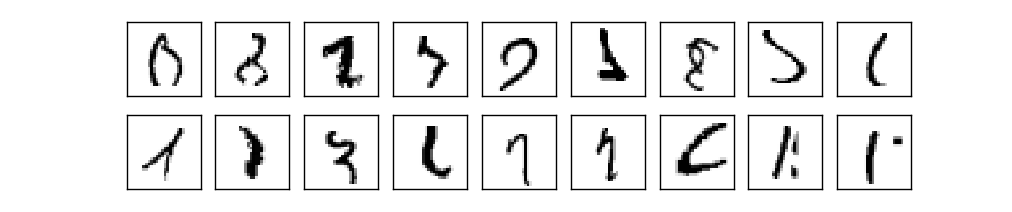
\includegraphics[height=64pt]{mnist_really_bad_images}
\end{center}

我相信你会同意那些数字很难辨认!考虑到 MNIST 数据集中这样的图像,神经网络能准确
识别 $10,000$ 幅测试图像中除了 $21$ 幅之外的其它所有图像,这表现得相当卓越。通常,
当编程时我们相信解决一个类似识别 MNIST 数字的问题需要一个复杂的算法。但是即使是
刚才提到的 Wan 等人的论文中用的神经网络,只涉及到相当简单的算法、和我们在这一章
中已经看到的算法的变化形式。所有的复杂性自动从训练数据学习。在某种意义上,我们的
结果和那些在更深奥的论文中都有的寓意是,对有些问题:

\begin{center}
  复杂的算法 $\leq$ 简单的学习算法 + 好的训练数据
\end{center}

\section{迈向深度学习}
\label{sec:toward_deep_learning}

虽然我们的神经网络给出了令人印象深刻的表现,但这样的表现带有几分神秘。网络中的权
重和偏置是被自动发现的。这意味着我们不能立即解释网络怎么做的、做了什么。我们能否
找到一些方法来理解我们的网络通过什么原理分类手写数字?并且,在知道了这些原理后,
我们能做得更好吗?

为了让这些问题更具体,我们假设数十年后神经网络引发了人工智能(AI)。到那个时候,
我们能明白这种智能网络的工作机制吗?或许,因为有着自动学习得到的权重和偏置,这些
是我们无法理解的,这样的神经网络对我们来说是不透明的。在人工智能的早期研究阶段,
人们希望在构建人工智能的努力过程中,也同时能够帮助我们理解智能背后的机制,以及人
类大脑的运转方式。但结果可能是我们既不能够理解大脑的机制,也不能够理解人工智能的
机制。

为解决这些问题,让我们重新思考一下我在本章开始时所给的人工神经元的解释,作为一种
衡量证据的方法。假设我们要确定一幅图像是否显示有人脸\footnote{照片来
  源:
  \href{http://commons.wikimedia.org/wiki/File:Kangaroo_ST_03.JPG}{1}. \href{http://commons.wikimedia.org/wiki/User:ST}{Ester
    Inbar}. \href{http://commons.wikimedia.org/wiki/File:Albert_Einstein_at_the_age_of_three_(1882).jpg}{2}. 未知. \href{http://commons.wikimedia.org/wiki/File:The_Hubble_eXtreme_Deep_Field.jpg}{3}. NASA,
  ESA, G. Illingworth, D. Magee, and P. Oesch (University of California, Santa
  Cruz), R. Bouwens (Leiden University), and the HUDF09 Team. 点击序号查看更多细
  节。}:
\begin{center}
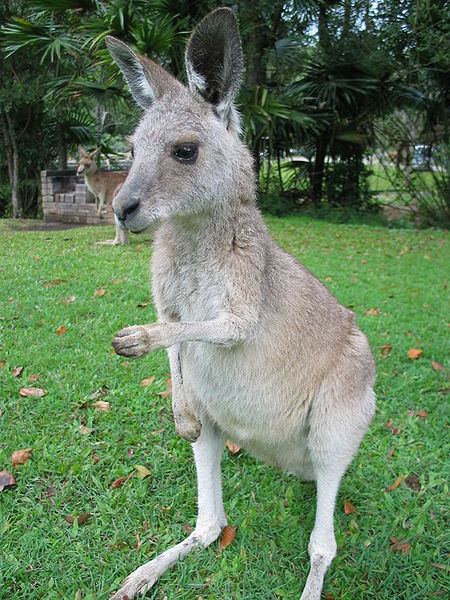
\includegraphics[height=125pt]{images/Kangaroo_ST_03}
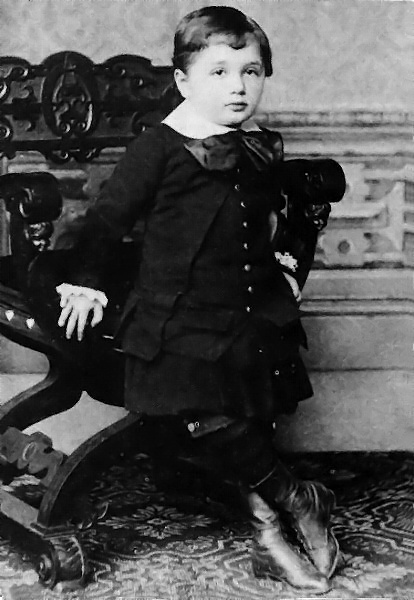
\includegraphics[height=125pt]{images/Albert_Einstein_at_the_age_of_three_(1882)}
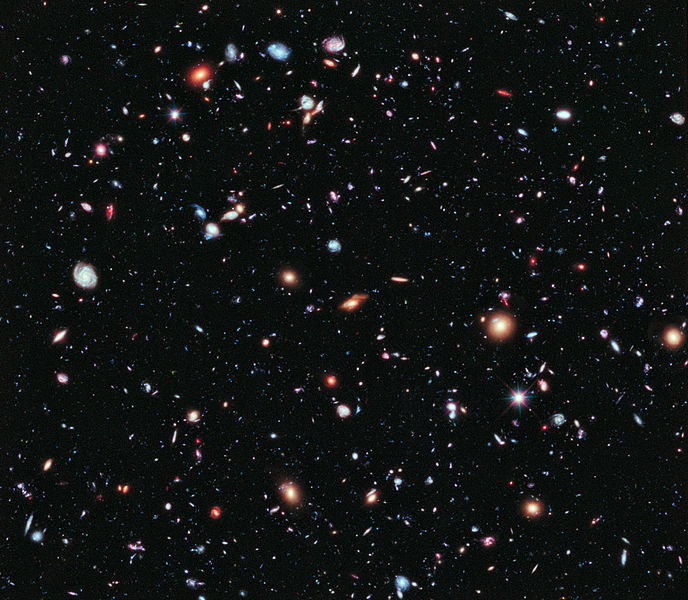
\includegraphics[height=125pt]{images/The_Hubble_eXtreme_Deep_Field}
\end{center}

我们可以用解决手写识别问题的相同方式来攻克这个问题~——~网络的输入是图像中的像素,
网络的输出是一个单个的神经元用于表明“是的,这是一张脸”或“不,这不是一张脸”。

假设我们就采取了这个方法,但接下来我们先不去使用一个学习算法。而是去尝试亲手设计
一个网络,并为它选择合适的权重和偏置。我们要怎样做呢?暂时先忘掉神经网络,我们受
到启发的一个想法是将这个问题分解成子问题:图像的左上角有一个眼睛吗?右上角有一个
眼睛吗?中间有一个鼻子吗?下面中央有一个嘴吗?上面有头发吗?诸如此类。

如果一些问题的回答是“是”,或者甚至仅仅是“可能是”,那么我们可以作出结论这个图
像可能是一张脸。相反地,如果大多数这些问题的答案是“不是”,那么这张图像可能不是
一张脸。

当然,这仅仅是一个粗略的想法,而且它存在许多缺陷。也许有个人是秃头,没有头发。也
许我们仅仅能看到脸的部分,或者这张脸是有角度的,因此一些面部特征是模糊的。不过这
个想法表明了如果我们能够使用神经网络来解决这些子问题,那么我们也许可以通过将这些
解决子问题的网络结合起来,构成一个人脸检测的神经网络。下图是一个可能的结构,其中
的方框表示子网络。注意,这不是一个人脸检测问题的现实的解决方法,而是为了帮助我们
构建起网络如何运转的直观感受。下图是这个网络的结构:

\begin{center}
  \includegraphics{tikz14}
\end{center}

子网络也可以被继续分解,这看上去很合理。假设我们考虑这个问题:“左上角有一个眼睛
吗?”。 这个问题可以被分解成这些子问题:“有一个眉毛吗?”,“有睫毛吗?”,
“有虹膜吗?”,等等。当然这些问题也应该包含关于位置的信息~——~诸如“在左上角有眉
毛,上面有虹膜吗?”~——~但是让我们先保持简单。回答问题“左上角有一个眼睛吗?”的
网络能够被分解成:

\begin{center}
  \includegraphics{tikz15}
\end{center}

这些子问题也同样可以继续被分解,并通过多个网络层传递得越来越远。最终,我们的子网
络可以回答那些只包含若干个像素点的简单问题。举例来说,这些简单的问题可能是询问图
像中的几个像素是否构成非常简单的形状。这些问题就可以被那些与图像中原始像素点相连
的单个神经元所回答。

最终的结果是,我们设计出了一个网络,它将一个非常复杂的问题~——~这张图像是否有一张
人脸~——~分解成在单像素层面上就可回答的非常简单的问题。它通过一系列多层结构来完成,
在前面的网络层,它回答关于输入图像非常简单明确的问题,在后面的网络层,它建立了一
个更加复杂和抽象的层级结构。包含这种多层结构~——~两层或更多隐藏层~——~的网络被称为%
\emph{深度神经网络}\index{深度神经网络}。

当然,我没有提到如何去递归地分解成子网络。手工设计网络中的权重和偏置无疑是不切实
际的。取而代之的是,我们希望使用学习算法来让网络能够自动从训练数据中学习权重和偏
差~——~这样,形成一个概念的层次结构。80 年代和 90 年代的研究人员尝试了使用随机梯
度下降和反向传播来训练深度网络。不幸的是,除了一些特殊的结构,他们并没有取得很好
的效果。虽然网络能够学习,但是学习速度非常缓慢,不适合在实际中使用。

自 2006 年以来,人们已经开发了一系列技术使深度神经网络能够学习。这些深度学习技术
基于随机梯度下降和反向传播,并引进了新的想法。这些技术已经使更深(更大)的网络能
够被训练~——~现在训练一个有 5 到 10 层隐藏层的网络都是很常见的。而且事实证明,在
许多问题上,它们比那些浅层神经网络,例如仅有一个隐藏层的网络,表现的更加出色。当
然,原因是深度网络能够构建起一个复杂的概念的层次结构。这有点像传统编程语言使用模
块化的设计和抽象的思想来创建复杂的计算机程序。将深度网络与浅层网络进行对比,有点
像将一个能够进行函数调用的程序语言与一个不能进行函数调用的精简语言进行对比。抽象
在神经网络中的形式和传统的编程方式相比不同,但它同样重要。


% file: chap2.tex

\chapter{反向传播算法如何工作}
\label{ch:HowTheBackpropagationAlgorithmWorks}

在\hyperref[ch:UsingNeuralNetsToRecognizeHandwrittenDigits]{上一章},我们看到了
神经网络如何使用梯度下降算法来学习他们自身的\gls*{weight}和\gls*{bias}。但是,这
里还留下了一个问题:我们并没有讨论如何计算代价函数的梯度。这是很大的缺失!在本章,
我们会解释计算这些梯度的快速算法,也就是\textbf{\gls{bp}}。

\gls*{bp}算法最初在 1970 年代被提及,但是人们直到
\href{http://en.wikipedia.org/wiki/David_Rumelhart}{David Rumelhart}、
\href{http://www.cs.toronto.edu/~hinton/}{Geoffrey Hinton} 和
\href{http://en.wikipedia.org/wiki/Ronald_J._Williams}{Ronald Williams} 的著名的
\href{http://www.nature.com/nature/journal/v323/n6088/pdf/323533a0.pdf}{1986年的
  论文}中才认识到这个算法的重要性。这篇论文描述了对一些神经网络反向传播要比传统
的方法更快,这使得使用神经网络来解决之前无法完成的问题变得可行。现在,反向传播算
法已经是神经网络学习的重要组成部分了。

本章在全书的范围内要比其他章节包含更多的数学内容。如果你不是对数学特别感兴趣,那
么可以跳过本章,将反向传播当成一个黑盒,忽略其中的细节。那么为何要研究这些细节呢?

答案当然是理解。\gls*{bp}的核心是一个对代价函数 $C$ 关于任何\gls*{weight} $w$
(或者\gls*{bias} $b$ )的偏导数 $\partial C/\partial w$ 的表达式。这个表达式告
诉我们在改变\gls*{weight}和\gls*{bias}时,代价函数变化的快慢。尽管表达式会有点复
杂,不过里面也包含一种美感,就是每个元素其实是拥有一种自然的直觉上的解释。所以%
\gls*{bp}不仅仅是一种学习的快速算法。实际上它让我们细致领悟如何通过改变%
\gls*{weight}和\gls*{bias}来改变整个网络的行为。因此,这也是学习\gls*{bp}细节的
重要价值所在。

如上面所说,如果你想要粗览本章,或者直接跳到下一章,都是可以的。剩下的内容即使你
是把\gls*{bp}看做黑盒也是可以掌握的。当然,后面章节中也会有部分内容涉及本章的结
论,所以会常常给出本章的参考。不过对这些知识点,就算你对推导的细节不太清楚你还是
应该要理解主要结论。

\section{热身:神经网络中使用矩阵快速计算输出的方法}
\label{sec:warm_up}

在讨论\gls*{bp}前,我们先熟悉一下基于矩阵的算法来计算网络的输出。事实上,我们在%
\hyperref[sec:implementing_our_network_to_classify_digits]{上一章的最后}已经能够
看到这个算法了,但是我在那里很快地略过了,所以现在让我们仔细讨论一下。特别地,这
样能够用相似的场景帮助我们熟悉在\gls*{bp}中使用的矩阵表示。

我们首先给出网络中\gls*{weight}的清晰定义。我们使用 $w^l_{jk}$ 表示从
$(l-1)^{\rm th}$ 层的 $k^{\rm th}$ 个神经元到 $l^{\rm th}$ 层的 $j^{\rm th}$ 个
神经元的链接上的\gls*{weight}。例如,下图给出了网络中第二层的第四个神经元到第三
层的第二个神经元的链接上的\gls*{weight}:

\begin{center}
  \includegraphics{tikz16}
\end{center}

这样的表示粗看比较奇怪,需要花一点时间消化。但是,后面你会发现这样的表示会比较方
便也很自然。奇怪的一点其实是下标 $j$ 和 $k$ 的顺序。你可能觉得反过来更加合理。但
我接下来会告诉你为什么要这样做。

我们对网络的\gls*{bias}和激活值也会使用类似的表示。显式地,我们使用 $b^l_j$ 表示
在 $l^{\rm th}$ 层第 $j^{\rm th}$ 个神经元的\gls*{bias},使用 $a^l_j$ 表示
$l^{\rm th}$ 层第 $j^{\rm th}$ 个神经元的激活值。下面的图清楚地解释了这样表示的
含义:

\begin{center}
  \includegraphics{tikz17}
\end{center}

有了这些表示,$l^{\rm th}$ 层的第 $j^{\rm th}$ 个神经元的激活值 $a^{l}_j$ 就和
$(l-1)^{\rm th}$ 层的激活值通过方程关联起来了(对比公式~\eqref{eq:4} 和上一章的
  讨论):
\begin{equation}
  a^{l}_j = \sigma\left( \sum_k w^{l}_{jk} a^{l-1}_k + b^l_j \right)
  \label{eq:23}\tag{23}
\end{equation}

其中求和是在 $(l-1)^{\rm th}$ 层的所有 $k$ 个神经元上进行的。为了用矩阵的形式重
写这个表达式,我们对每一层 $l$ 都定义一个\textbf{\gls*{weight}矩阵} $w^l$。%
\gls*{weight}矩阵 $w^l$ 的元素正是连接到 $l^{\rm th}$ 层神经元的\gls*{weight},
更确切地说,在第$j^{\rm th}$ 行第 $k^{\rm th}$ 列的元素是 $w^l_{jk}$。类似的,对
每一层 $l$,定义一个\textbf{\gls*{bias}向量},$b^l$。你已经猜到这些如何工作
了~——~\gls*{bias}向量的每个元素其实就是前面给出的 $b^l_j$,每个元素对应于
$l^{\rm th}$ 层的每个神经元。最后,我们定义激活向量 $a^l$,其元素是那些激活值
$a^l_j$。

最后我们需要引入向量化函数(如 $\sigma$)来按照矩阵形式重写公式~\eqref{eq:23}。
在上一章,我们其实已经碰到向量化了,其含义就是作用函数(如 $\sigma$)到向量 $v$
中的每个元素。我们使用 $\sigma(v)$ 表示这种按元素进行的函数作用。所以,
$\sigma(v)$ 的每个元素其实满足 $\sigma(v)_j = \sigma(v_j)$。给个例子,如果我们的
作用函数是 $f(x) = x^2$,那么向量化的 $f$ 的函数作用就起到下面的效果:
\begin{equation}
  f\left(\left[ \begin{array}{c} 2 \\ 3 \end{array} \right] \right)
  = \left[ \begin{array}{c} f(2) \\ f(3) \end{array} \right]
  = \left[ \begin{array}{c} 4 \\ 9 \end{array} \right]
\label{eq:24}\tag{24}
\end{equation}
也就是说,向量化的 $f$ 仅仅是对向量的每个元素进行了平方运算。

了解了这些表示,方程~\eqref{eq:23} 就可以写成下面这种美妙而简洁的向量形式了:
\begin{equation}
  a^{l} = \sigma(w^l a^{l-1}+b^l)
  \label{eq:25}\tag{25}
\end{equation}

这个表达式给出了一种更加全局的思考每层的激活值和前一层激活值的关联方式:我们仅仅
用\gls*{weight}矩阵作用在激活值上,然后加上一个\gls*{bias}向量,最后作用
$\sigma$ 函数
\footnote{其实,这就是让我们使用之前的矩阵下标 $w_{jk}^l$ 表示的初因。如果我们使
  用 $j$ 来索引输入神经元,$k$ 索引输出神经元,那么在方程~\eqref{eq:25} 中我们需
  要将这里的矩阵换做其转置。这是一个小的改变,但是令人困惑,这会使得我们无法自然
  地讲出(思考)“应用\gls*{weight}矩阵到激活值上”这样的简单的表达。}。这种全局的观点相
比神经元层面的观点常常更加简明(没有更多的索引下标了!)。把它看做是在保留清晰认
识的前提下逃离下标困境的方法。在实践中,表达式同样很有用,因为大多数矩阵库提供了
实现矩阵乘法、向量加法和向量化的快速方法。实际上,上一章的%
\hyperref[sec:implementing_our_network_to_classify_digits]{代码}其实已经隐式使用
了这种表达式来计算网络行为。

在使用方程~\eqref{eq:25} 计算 $a^l$ 的过程中,我们计算了中间量 $z^l \equiv w^l
a^{l-1}+b^l$。这个量其实是非常有用的:我们称 $z^l$ 为 $l$ 层神经元的\textbf{带权
  输入}\index{带权输入}。在本章后面,我们会充分利用带权输入 $z^l$。方
程~\eqref{eq:25} 有时候会以带权输入的形式写作 $a^l = \sigma(z^l)$。同样要指出的
是 $z^l$ 的每个元素是 $z^l_j = \sum_k w^l_{jk} a^{l-1}_k+b^l_j$,其实 $z^l_j$ 就
是第 $l$ 层第 $j$ 个神经元的激活函数的带权输入。

\section{关于代价函数的两个假设}
\label{sec:TwoAssumptionsWeNeedAboutTheCostFunction}

\gls*{bp}的目标是计算代价函数 $C$ 分别关于 $w$ 和 $b$ 的偏导数 $\partial
C/\partial w$ 和 $\partial C / \partial b$。为了让\gls*{bp}可行,我们需要做出关
于代价函数的两个主要假设。在给出这两个假设之前,我们先看看具体的一个代价函数。我
们会使用上一章使用的二次代价函数(参见方程~\eqref{eq:6})。按照上一节给出的表示,
二次代价函数有下列形式:
\begin{equation}
  C = \frac{1}{2n} \sum_x \|y(x)-a^L(x)\|^2
  \label{eq:26}\tag{26}
\end{equation}
其中 $n$ 是训练样本的总数;求和运算遍历了每个训练样本 $x$;$y = y(x)$ 是对应的目
标输出;$L$ 表示网络的层数;$a^L = a^L(x)$ 是当输入是 $x$ 时的网络输出的激活值向
量。

好了,为了应用\gls*{bp},我们需要对代价函数 $C$ 做出什么样的前提假设呢?第一个假
设就是代价函数可以被写成一个在每个训练样本 $x$ 上的代价函数 $C_x$ 的均值
$C=\frac{1}{n} \sum_x C_x$。这是关于二次代价函数的例子,其中对每个独立的训练样本
其代价是 $C_x = \frac{1}{2} ||y-a^L||^2$。这个假设对书中提到的其他任何一个代价函
数也都是必须满足的。

需要这个假设的原因是\gls*{bp}实际上是对一个独立的训练样本计算了 $\partial
C_x/\partial w$ 和 $\partial C_x/\partial b$。然后我们通过在所有训练样本上进行平
均化获得 $\partial C/\partial w$ 和 $\partial C/\partial b$。实际上,有了这个假
设,我们会认为训练样本 $x$ 已经被固定住了,丢掉了其下标,将代价函数 $C_x$ 看做
$C$。最终我们会把下标加上,现在为了简化表示其实没有这个必要。

第二个假设就是代价可以写成神经网络输出的函数:

\begin{center}
  \includegraphics{tikz18}
\end{center}

例如,二次代价函数满足这个要求,因为对于一个单独的训练样本 $x$ 其二次代价函数可
以写作:
\begin{equation}
  C = \frac{1}{2} \|y-a^L\|^2 = \frac{1}{2} \sum_j (y_j-a^L_j)^2
  \label{eq:27}\tag{27}
\end{equation}
这是输出的激活值的函数。当然,这个代价函数同样还依赖于目标输出 $y$,你可能奇怪为
什么我们不把代价也看作一个 $y$ 的函数。记住,输入的训练样本 $x$ 是固定的,所以输
出 $y$ 同样是一个固定的参数。尤其是它并不是可以随意通过改变\gls*{weight}和%
\gls*{bias}来改变的,也就是说,这不是神经网络学习的对象。所以,将 $C$ 看成仅有输
出激活值 $a^L$ 的函数才是合理的,而 $y$ 仅仅是帮助定义函数的参数而已。

\section{Hadamard 乘积,$s \odot t$}
\label{sec:the_hadamard_product}

\gls*{bp}算法基于常规的线性代数运算~——~诸如向量加法,向量矩阵乘法等。但是有一个
运算不大常见。特别地,假设 $s$ 和 $t$ 是两个同样维度的向量。那么我们使用 $s\odot
t$ 来表示\textbf{按元素}的乘积。所以 $s\odot t$ 的元素就是 $(s\odot t)_j = s_j
t_j$。给个例子,
\begin{equation}
  \left[\begin{array}{c} 1 \\ 2 \end{array}\right]
  \odot \left[\begin{array}{c} 3 \\ 4\end{array} \right]
  = \left[ \begin{array}{c} 1 * 3 \\ 2 * 4 \end{array} \right]
  = \left[ \begin{array}{c} 3 \\ 8 \end{array} \right]
  \label{eq:28}\tag{28}
\end{equation}

这种类型的按元素乘法有时候被称为\textbf{Hadamard 乘积},或者\textbf{Schur 乘积}。
我们这里取前者。好的矩阵库通常会提供 Hadamard 乘积的快速实现,在实现\gls*{bp}的
时候用起来很方便。

\section{反向传播的四个基本方程}
\label{sec:the_four_fundamental_equations_behind_backpropagation}

\gls*{bp}其实是对\gls*{weight}和\gls*{bias}变化影响代价函数过程的理解。最终极的
含义其实就是计算偏导数 $\partial C/\partial w_{jk}^l$ 和 $\partial C/\partial
b_j^l$。但是为了计算这些值,我们首先引入一个中间量,$\delta_j^l$,这个我们称为在
$l^{th}$ 层第 $j^{th}$ 个神经元上的\textbf{\gls{error}}。

\gls*{bp}将给出计算误差 $\delta_j^l$ 的流程,然后将其关联到计算 $\partial
C/\partial w_{jk}^l$ 和 $\partial C/\partial b_j^l$ 上。

为了理解误差是如何定义的,假设在神经网络上有一个调皮鬼:

\begin{center}
  \includegraphics{tikz19}
\end{center}

这个调皮鬼在 $l$ 层的第 $j^{th}$ 个神经元上。当输入进来时,调皮鬼对神经元的操作
进行搅局。他会增加很小的变化 $\Delta z_j^l$ 在神经元的带权输入上,使得神经元输出
由 $\sigma(z_j^l)$ 变成 $\sigma(z_j^l + \Delta z_j^l)$。这个变化会向网络后面的层
进行传播,最终导致整个代价产生 $\frac{\partial C}{\partial z_j^l} \Delta z_j^l$
的改变。

现在,这个调皮鬼变好了,试着帮助你来优化代价,它试着找到可以让代价更小的$\Delta
z_j^l$。假设 $\frac{\partial C}{\partial z_j^l}$ 有一个很大的值(或正或负)。那
么这个调皮鬼可以通过选择与 $\frac{\partial C}{\partial z_j^l}$ 相反符号的
$\Delta z_j^l$ 来降低代价。相反,如果 $\frac{\partial C}{\partial z_j^l}$接近
$0$,那么调皮鬼并不能通过扰动带权输入 $z_j^l$ 来改善太多代价。在调皮鬼看来,这时
候神经元已经很接近最优了\footnote{这里需要注意的是,只有在 $\Delta z_j^l$ 很小的
  时候才能够满足。我们需要假设调皮鬼只能进行微小的调整。}。所以这里有一种启发式
的认识,$\frac{\partial C}{\partial z_j^l}$ 是神经元的误差的度量。

按照上面的描述,我们定义 $l$ 层的第 $j^{th}$ 个神经元上的误差 $\delta_j^l$ 为:
\begin{equation}
  \delta^l_j \equiv \frac{\partial C}{\partial z^l_j}
  \label{eq:29}\tag{29}
\end{equation}

按照我们通常的惯例,我们使用 $\delta^l$ 表示关联于 $l$ 层的误差向量。\gls*{bp}会
提供给我们一种计算每层的 $\delta^l$ 的方法,然后将这些误差和最终我们需要的量
$\partial C/\partial w_{jk}^l$ 和 $\partial C/\partial b_j^l$ 联系起来。

你可能会想知道为何这个调皮鬼在改变带权输入 $z_j^l$。把它想象成改变输出激活值
$a_j^l$ 肯定会更加自然,然后就使用 $\frac{\partial C}{\partial a_j^l}$ 作为度量
误差的方法了。实际上,如果你这样做的话,其实和下面要讨论的差不多。但是看起来,前
面的方法会让\gls*{bp}在代数运算上变得比较复杂。所以我们坚持使用 $\delta_j^l =
\partial C / \partial z_j^l$ 作为误差的度量\footnote{在分类问题中,误差有时候会
  用作分类的错误率。如果神经网络正确分类了 96.0\% 的数字,那么其误差是 4.0\%。很
  明显,这和我们上面提及的误差的差别非常大了。在实际应用中,区分这两种含义是非常
  容易的。}。\\

\textbf{解决方案:} \gls*{bp}基于四个基本方程。这些方程给我们一种计算误差
$\delta^l$ 和代价函数梯度的方法。我列出这四个方程。但是需要注意:你不需要一下子
能够同时理解这些公式。希望越大失望越大。实际上,\gls*{bp}方程内容很多,完全理解
这些需要花费充分的时间和耐心,需要一步一步地深入理解。而好的消息是,这样的付出回
报巨大。所以本节对这些内容的讨论仅仅是一个帮助你正确掌握这些方程的起步。

下面简要介绍我们的探讨这些公式的计划:首先%
\hyperref[sec:proof_of_the_four_fundamental_equations]{给出这些公式的简短证明}以
解释他们的正确性;然后以伪代码的方式%
\hyperref[sec:the_backpropagation_algorithm]{给出这些公式的算法形式},并%
\hyperref[sec:the_code_for_backpropagation]{展示}这些伪代码如何转化成真实的可执
行的 Python 代码;在\hyperref[sec:backpropagation_the_big_picture]{本章的最后},
我们会发展出一个关于\gls*{bp}方程含义的直觉画面,以及人们如何能够从零开始发现这
个规律。按照此法,我们会不断地提及这四个基本方程,随着你对这些方程理解的加深,他
们会看起来更加舒服,甚至是美妙和自然的。\\

\textbf{输出层误差的方程,$\delta^L$:} 每个元素定义如下:
\begin{equation}
  \delta^L_j = \frac{\partial C}{\partial a^L_j} \sigma'(z^L_j)
  \label{eq:bp1}\tag{BP1}
\end{equation}

这是一个非常自然的表达式。右式第一个项 $\partial C/\partial a_j^L$ 表示代价随着
$j^{th}$ 输出激活值的变化而变化的速度。假如 $C$ 不太依赖一个特定的输出神经元 $j$,
那么 $\delta_j^L$ 就会很小,这也是我们想要的效果。右式第二项 $\sigma'(z_j^L)$ 刻
画了在 $z_j^L$ 处激活函数 $\sigma$ 变化的速度。

注意到在 \eqref{eq:bp1} 中的每个部分都是很好计算的。特别地,我们在计算网络行为时
计算 $z_j^L$,这仅仅需要一点点额外工作就可以计算 $\sigma'(z_j^L)$。当然
$\partial C/\partial a_j^L$ 依赖于代价函数的形式。然而,给定了代价函数,计算
$\partial C/\partial a_j^L$ 就没有什么大问题了。例如,如果我们使用二次函数,那么
$C = \frac{1}{2} \sum_j(y_j-a_j)^2$,所以 $\partial C/\partial a_j^L = (a_j -
y_j)$,这其实很容易计算。

方程~\eqref{eq:bp1} 对 $\delta^L$ 来说是个按分量构成的表达式。这是一个非常好的表
达式,但不是我们期望的用矩阵表示的形式。但是,以矩阵形式重写方程其实很简单,
\begin{equation}
  \delta^L = \nabla_a C \odot \sigma'(z^L)
  \label{eq:bp1a}\tag{BP1a}
\end{equation}

这里 $\nabla_a C$ 被定义成一个向量,其元素是偏导数 $\partial C/\partial a_j^L$。
你可以将 $\nabla_a C$ 看成是 $C$ 关于输出激活值的改变速度。方程~\eqref{eq:bp1}和
方程~\eqref{eq:bp1a} 的等价也是显而易见的,所以现在开始,我们会用\eqref{eq:bp1}
表示这两个方程。举个例子,在二次代价函数时,我们有 $\nabla_a C = (a^L - y)$,所
以 \eqref{eq:bp1} 的整个矩阵形式就变成
\begin{equation}
  \delta^L = (a^L-y) \odot \sigma'(z^L)
  \label{eq:30}\tag{30}
\end{equation}

如你所见,这个方程中的每个项都有一个很好的向量形式,所以也可以很方便地使用像
Numpy 这样的矩阵库进行计算了。\\

\textbf{使用下一层的误差 $\delta^{l+1}$ 来表示当前层的误差 $\delta^l$:} 特别地,
\begin{equation}
  \delta^l = ((w^{l+1})^T \delta^{l+1}) \odot \sigma'(z^l)
  \label{eq:bp2}\tag{BP2}
\end{equation}
其中 $(w^{l+1})^T$ 是 $(l+1)^{\rm th}$ 层\gls*{weight}矩阵 $w^{l+1}$ 的转置。这
个公式看上去有些复杂,但每一个元素有很好的解释。假设我们知道 $l+1^{\rm th}$ 层的
误差 $\delta^{l+1}$。当我们应用转置的\gls*{weight}矩阵 $(w^{l+1})^T$,我们可以凭
直觉地把它看作是在沿着网络\textbf{反向}移动误差,给了我们度量在 $l^{\rm th}$ 层
输出的误差方法。然后,我们进行 Hadamard 乘积运算 $\odot \sigma'(z^l)$。这会让误
差通过 $l$ 层的激活函数反向传递回来并给出在第 $l$ 层的带权输入的误差 $\delta$。

通过组合 \eqref{eq:bp1} 和 \eqref{eq:bp2},我们可以计算任何层的误差 $\delta^l$。
首先使用 \eqref{eq:bp1} 计算 $\delta^L$,然后应用方程~\eqref{eq:bp2} 来计算
$\delta^{L-1}$,然后再次用方程~\eqref{eq:bp2} 来计算 $\delta^{L-2}$,如此一步一
步地\gls*{bp}完整个网络。\\

\textbf{代价函数关于网络中任意\gls*{bias}的改变率:} 就是
\begin{equation}
  \frac{\partial C}{\partial b^l_j} = \delta^l_j
  \label{eq:bp3}\tag{BP3}
\end{equation}

这其实是,误差 $\delta^l_j$ 和偏导数值 $\partial C / \partial b^l_j$ \textbf{完
  全一致}。这是很好的性质,因为 \eqref{eq:bp1} 和 \eqref{eq:bp2} 已经告诉我们如
何计算 $\delta^l_j$。所以就可以将 \eqref{eq:bp3} 简记为
\begin{equation}
  \frac{\partial C}{\partial b} = \delta
  \label{eq:31}\tag{31}
\end{equation}
其中 $\delta$ 和\gls*{bias} $b$ 都是针对同一个神经元。\\

\textbf{代价函数关于任何一个\gls*{weight}的改变率:} 特别地,
\begin{equation}
  \frac{\partial C}{\partial w^l_{jk}} = a^{l-1}_k \delta^l_j
  \label{eq:bp4}\tag{BP4}
\end{equation}

这告诉我们如何计算偏导数 $\partial C/\partial w_{jk}^l$,其中 $\delta^l$ 和
$a^{l-1}$ 这些量我们都已经知道如何计算了。方程也可以写成下面用更少下标的表示:
\begin{equation}
  \frac{\partial
    C}{\partial w} = a_{\rm in} \delta_{\rm out}
  \label{eq:32}\tag{32}
\end{equation}
其中 $a_{\rm in}$ 是输入给\gls*{weight} $w$ 的神经元的激活值,$\delta_{\rm out}$
是输出自\gls*{weight} $w$ 的神经元的误差。放大看看\gls*{weight} $w$,还有两个由
这个\gls*{weight}相连的神经元,我们给出一幅图如下:

\begin{center}
  \includegraphics{tikz20}
\end{center}

方程~\eqref{eq:32} 的一个好的结果就是当激活值 $a_{\rm in}$ 很小,$a_{\rm in}
\approx 0$,梯度 $\partial C/\partial w$ 也会趋向很小。这样,我们就说%
\gls*{weight}\textbf{缓慢学习},表示在梯度下降的时候,这个\gls*{weight}不会改变
太多。换言之,\eqref{eq:bp4} 的一个结果就是来自低激活值神经元的\gls*{weight}学习
会非常缓慢。

这四个公式 \eqref{eq:bp1}--\eqref{eq:bp4} 同样还有其它可以理解的方面。让我们从输
出层开始,先看看~\eqref{eq:bp1} 中的项$\sigma'(z_k^l)$。回忆一下%
\hyperref[fig:StepFunction]{上一章中S型函数的图形},当 $\sigma(z^L_j)$ 近似为$0$
或者 $1$ 的时候 $\sigma$ 函数变得非常平。这时 $\sigma'(z^L_j) \approx 0$。所以如
果输出神经元处于或者低激活值($\approx 0$)或者高激活值($\approx 1$)时,最终层
的\gls*{weight}学习缓慢。这样的情形,我们常常称输出神经元已经\textbf{饱和}\index{饱
  和}了,并且,\gls*{weight}学习也会终止(或者学习非常缓慢)。类似的结果对于输出
神经元的\gls*{bias}也是成立的。

针对前面的层,我们也有类似的观点。特别地,注意在 \eqref{eq:bp2} 中的项
$\sigma'(z^l)$。这表示如果神经元已经接近饱和,$\delta_j^l$ 很可能变小。这就导致
任何输入进一个饱和的神经元的\gls*{weight}学习缓慢\footnote{如果 ${w^{l+1}}^T
  \delta^{l+1}$ 拥有足够大的量能够补偿 $\sigma'(z_k^l)$ 的话,这里的推导就不能成
  立了。但是我们上面是常见的情形。}。

总结一下,我们已经学习到,如果输入神经元激活值很低,或者输出神经元已经饱和了(过
  高或者过低的激活值),\gls*{weight}会学习缓慢。

这些观测其实也不是非常出于意料的。不过,他们帮助我们完善了关于神经网络学习的背后
的思维模型。而且,我们可以将这种推断方式进行推广。四个基本方程也其实对任何的激活
函数都是成立的(证明中也可以看到,其实推断本身不依赖于任何具体的代价函数)所以,
我们可以使用这些方程来\textbf{设计}有特定学习属性的激活函数。我们这里给个例子,
假设我们准备选择一个(非S型)激活函数 $\sigma$ 使得 $\sigma'$ 总是正数,并且不会
趋近 $0$。这会防止在原始的S型神经元饱和时学习速度下降的情况出现。在本书的后面,
我们会见到这种类型的对激活函数的改变。时时回顾这四个方程
\eqref{eq:bp1}--\eqref{eq:bp4} 可以帮助解释为何需要有这些尝试,以及尝试带来的影
响。

\begin{center}
  \begin{minipage}{0.7\textwidth}
    \begin{framed}
      \centering
      \textbf{总结:\gls*{bp}的四个方程式}\index{\gls*{bp}的四个方程式}\label{backpropsummary}\\
      \vspace{1.5ex}
      \begin{tabular}{ll}
        $\delta^L = \nabla_a C \odot \sigma'(z^L)$            & \hspace{2cm}\eqref{eq:bp1} \\[1.5ex]
        $\delta^l = ((w^{l+1})^T \delta^{l+1}) \odot \sigma'(z^l)$ & \hspace{2cm}\eqref{eq:bp2} \\[1.5ex]
        $\frac{\partial C}{\partial b^l_j} = \delta^l_j$       & \hspace{2cm}\eqref{eq:bp3} \\[1.5ex]
        $\frac{\partial C}{\partial w^l_{jk}} = a^{l-1}_k \delta^l_j$ & \hspace{2cm}\eqref{eq:bp4}
      \end{tabular}
    \end{framed}
  \end{minipage}
\end{center}

\subsection*{问题}

\begin{itemize}
\item \textbf{另一种\gls*{bp}方程的表示方式:} 我已经给出了使用 Hadamard 乘积的反
  向传播的公式(尤其是 \eqref{eq:bp1} 和 \eqref{eq:bp2})。如果你对这种特殊的乘
  积不熟悉,可能会有一些困惑。下面还有一种表示方式,那就是基于传统的矩阵乘法,某
  些读者可能会觉得很有启发。(1)证明 \eqref{eq:bp1} 可以写成
  \begin{equation}
    \delta^L = \Sigma'(z^L) \nabla_a C
    \label{eq:33}\tag{33}
  \end{equation}
  其中 $\Sigma'(z^L)$ 是一个方阵,其对角线的元素是 $\sigma'(z_j^L)$,其他的元素
  均是 $0$。注意,这个矩阵通过一般的矩阵乘法作用在 $\nabla_a C$ 上。(2)证明
  \eqref{eq:bp2} 可以写成
  \begin{equation}
    \delta^l = \Sigma'(z^l) (w^{l+1})^T \delta^{l+1}
    \label{eq:34}\tag{34}
  \end{equation}
  (3)结合(1)和(2)证明
  \begin{equation}
    \delta^l = \Sigma'(z^l) (w^{l+1})^T \ldots \Sigma'(z^{L-1}) (w^L)^T
    \Sigma'(z^L) \nabla_a C
    \label{eq:35}\tag{35}
  \end{equation}
  对那些习惯于这种形式的矩阵乘法的读者,\eqref{eq:bp1} \eqref{eq:bp2} 应该更加容
  易理解。而我们坚持使用 Hadamard 乘积的原因在于其更快的数值实现。
\end{itemize}

\section{四个基本方程的证明(可选)}
\label{sec:proof_of_the_four_fundamental_equations}

我们现在证明这四个基本的方程 \eqref{eq:bp1}--\eqref{eq:bp4}。所有这些都是多元微
积分的\href{https://en.wikipedia.org/wiki/Chain_rule}{链式法则}\index{链式法则}%
的推论。如果你熟悉链式法则,那么我鼓励你在读之前尝试自己推导。

让我们从方程~\eqref{eq:bp1} 开始,它给出了输出误差 $\delta^L$ 的表达式。为了证明
这个方程,回忆下定义:
\begin{equation}
  \delta^L_j = \frac{\partial C}{\partial z^L_j}
\label{eq:36}\tag{36}
\end{equation}

应用链式法则,我们可以就输出激活值的偏导数的形式重新表示上面的偏导数:
\begin{equation}
  \delta^L_j = \sum_k \frac{\partial C}{\partial a^L_k} \frac{\partial a^L_k}{\partial z^L_j}
\label{eq:37}\tag{37}
\end{equation}
这里求和是在输出层的所有神经元 $k$ 上运行的。当然,第 $k^{\rm th}$ 个神经元的输
出激活值 $a^L_k$ 只依赖于当 $k=j$ 时第 $j^{\rm th}$ 个神经元的输入\gls*{weight}
$z^L_j$。所以当 $k \neq j$ 时 $\partial a^L_k / \partial z^L_j$ 消失了。结果我们
可以简化上一个方程为:
\begin{equation}
  \delta^L_j = \frac{\partial C}{\partial a^L_j} \frac{\partial a^L_j}{\partial z^L_j}
\label{eq:38}\tag{38}
\end{equation}

回想下 $a^L_j = \sigma(z^L_j)$,右边的第二项可以写为 $\sigma'(z^L_j)$,方程变成:
\begin{equation}
  \delta^L_j = \frac{\partial C}{\partial a^L_j} \sigma'(z^L_j)
\label{eq:39}\tag{39}
\end{equation}
这正是分量形式的~\eqref{eq:bp1}。

下一步,我们将证明~\eqref{eq:bp2},它给出了以下一层误差 $\delta^{l+1}$ 的形式表
示误差 $\delta^l$。为此,我们想要以 $\delta^{l+1}_k = \partial C / \partial
z^{l+1}_k$ 的形式重写 $\delta^l_j = \partial C / \partial z^l_j$。我们可以用链式
法则:
\begin{align}
  \delta^l_j &= \frac{\partial C}{\partial z^l_j} \label{eq:40}\tag{40}\\
             &= \sum_k \frac{\partial C}{\partial z^{l+1}_k} \frac{\partial z^{l+1}_k}{\partial z^l_j} \label{eq:41}\tag{41}\\
             &= \sum_k \frac{\partial z^{l+1}_k}{\partial z^l_j} \delta^{l+1}_k \label{eq:42}\tag{42}
\end{align}
这里最后一行我们交换了右边的两项,并用 $\delta^{l+1}_k$ 的定义代入。为了对最后一
行的第一项求值,注意:
\begin{equation}
  z^{l+1}_k = \sum_j w^{l+1}_{kj} a^l_j +b^{l+1}_k = \sum_j w^{l+1}_{kj} \sigma(z^l_j) +b^{l+1}_k
\label{eq:43}\tag{43}
\end{equation}

做微分,我们得到
\begin{equation}
  \frac{\partial z^{l+1}_k}{\partial z^l_j} = w^{l+1}_{kj} \sigma'(z^l_j)
\label{eq:44}\tag{44}
\end{equation}

把它代入~\eqref{eq:42} 我们得到
\begin{equation}
  \delta^l_j = \sum_k w^{l+1}_{kj}  \delta^{l+1}_k \sigma'(z^l_j)
\label{eq:45}\tag{45}
\end{equation}

这正是以分量形式写的~\eqref{eq:bp2}。

我们想证明的最后两个方程是~\eqref{eq:bp3} 和~\eqref{eq:bp4}。它们同样遵循链式法
则,和前面两个方程的证明相似。我把它们留给你做为练习。

\subsection*{练习}

\begin{itemize}
\item 证明方程~\eqref{eq:bp3} 和~\eqref{eq:bp4}。
\end{itemize}

这样我们就完成了\gls*{bp}四个基本公式的证明。证明本身看起来复杂。但是实际上就是
细心地应用链式法则。我们可以将\gls*{bp}看成是一种系统性地应用多元微积分中的链式
法则来计算代价函数的梯度的方式。这些就是\gls*{bp}理论上的内容~——~剩下的是实现细
节。

\section{反向传播算法}
\label{sec:the_backpropagation_algorithm}

\gls*{bp}方程给出了一种计算代价函数梯度的方法。让我们显式地用算法描述出来:

\begin{enumerate}
\item \textbf{输入 $x$:} 为输入层设置对应的激活值 $a^{1}$ 。
\item \textbf{前向传播:} 对每个 $l=2,3,...,L$ 计算相应的 $z^l = w^la^{l-1} +
  b^l$ 和 $a^l = \sigma(z^l)$
\item \textbf{输出层误差 $\delta^L$:} 计算向量 $\delta^L = \nabla_a C \odot
  \sigma'(z^L)$
\item \textbf{反向误差传播:} 对每个 $l=L-1, L-2,...,2$,计算
  $\delta^l = ((w^{l+1})^T\delta^{l+1})\odot \sigma'(z^l)$
\item \textbf{输出:} 代价函数的梯度由 $\frac{\partial C}{\partial w^l_{jk}} =
  a^{l-1}_k \delta^l_j$ 和 $\frac{\partial C}{\partial b_j^l} = \delta_j^l$ 得出
\end{enumerate}

检视这个算法,你可以看到为何它被称作\textbf{反向}传播。我们从最后一层开始向后计
算误差向量 $\delta^l$。这看起来有点奇怪,为何要从后面开始。但是如果你认真思考反
向传播的证明,这种反向移动其实是代价函数是网络输出的函数的结果。为了理解代价随前
面层的\gls*{weight}和\gls*{bias}变化的规律,我们需要重复作用链式法则,反向地获得
需要的表达式。

\subsection*{练习}

\begin{itemize}
\item \textbf{使用单个修正的神经元的\gls*{bp}}\quad 假设我们改变一个前馈网络中的
  单个神经元,使得那个神经元的输出是 $f(\sum_j w_jx_j + b)$,其中 $f$ 是和 S 型
  函数不同的某一函数。我们如何调整\gls*{bp}算法?
\item \textbf{线性神经元上的\gls*{bp}}\quad 假设我们将非线性神经元的 $\sigma$ 函
  数替换为 $\sigma(z) = z$。重写\gls*{bp}算法。
\end{itemize}

正如我们上面所讲的,\gls*{bp}算法对一个训练样本计算代价函数的梯度,$C=C_x$。在实
践中,通常将\gls*{bp}算法和诸如随机梯度下降这样的学习算法进行组合使用,我们会对
许多训练样本计算对应的梯度。特别地,给定一个大小为 $m$ 的\gls*{mini-batch},下面
的算法在这个\gls*{mini-batch}的基础上应用一步梯度下降学习算法:

\begin{enumerate}
\item \textbf{输入训练样本的集合}
\item \textbf{对每个训练样本 $x$:} 设置对应的输入激活 $a^{x,1}$,并执行下面的步
  骤:
  \begin{itemize}
  \item \textbf{前向传播:} 对每个 $l=2,3,...,L$ 计算 $z^{x,l} = w^la^{x,l-1} +
    b^l$ 和 $a^{x,l} = \sigma(z^{x,l})$。
  \item \textbf{输出误差 $\delta^{x,L}$:} 计算向量
    $\delta^{x,L} = \nabla_a C_x \odot \sigma'(z^{x,L})$。
  \item \textbf{\gls*{bp}误差:} 对每个 $l=L-1, L-2, ..., 2$ 计算
    $\delta^{x,l} = ((w^{l+1})^T\delta^{x,l+1})\odot \sigma'(z^{x,l})$。
  \end{itemize}
\item \textbf{梯度下降:} 对每个 $l=L-1, L-2, ..., 2$ 根据 $w^l \rightarrow w^l
  - \frac{\eta}{m}\sum_x \delta^{x,l}(a^{x,l-1})^T$ 和 $b^l \rightarrow b^l -
  \frac{\eta}{m}\sum_x \delta^{x,l}$ 更新\gls*{weight}和\gls*{bias}。
\end{enumerate}

当然,在实践中实现随机梯度下降,我们还需要一个产生训练样本的\gls*{mini-batch}的
循环,还有就是多重\gls*{epoch}的循环。这里我们先省略了。

\section{代码}
\label{sec:the_code_for_backpropagation}

理解了抽象的\gls*{bp}的理论知识,我们现在就可以学习上一章中使用的实现\gls*{bp}的
代码了。回想\hyperref[sec:implementing_our_network_to_classify_digits]{上一章}的
代码,需要研究的是在 \lstinline!Network! 类中的 \lstinline!update_mini_batch! 和
\lstinline!backprop! 方法。这些方法的代码其实是我们上面的算法描述的直接翻版。特
别地,\lstinline!update_mini_batch! 方法通过计算当前 \lstinline!mini_batch! 中的
训练样本对 \lstinline!Network! 的\gls*{weight}和\gls*{bias}进行了更新:

\begin{lstlisting}[language=Python]
class Network(object):
...
    def update_mini_batch(self, mini_batch, eta):
        """Update the network's weights and biases by applying
        gradient descent using backpropagation to a single mini batch.
        The "mini_batch" is a list of tuples "(x, y)", and "eta"
        is the learning rate."""
        nabla_b = [np.zeros(b.shape) for b in self.biases]
        nabla_w = [np.zeros(w.shape) for w in self.weights]
        for x, y in mini_batch:
            delta_nabla_b, delta_nabla_w = self.backprop(x, y)
            nabla_b = [nb+dnb for nb, dnb in zip(nabla_b, delta_nabla_b)]
            nabla_w = [nw+dnw for nw, dnw in zip(nabla_w, delta_nabla_w)]
        self.weights = [w-(eta/len(mini_batch))*nw
                        for w, nw in zip(self.weights, nabla_w)]
        self.biases = [b-(eta/len(mini_batch))*nb
                       for b, nb in zip(self.biases, nabla_b)]
\end{lstlisting}

主要工作其实是在 \lstinline!delta_nabla_b!,%
\lstinline!delta_nabla_w = self.backprop(x, y)! 这里完成的,调用了
\lstinline!backprop! 方法计算出了偏导数,
$\partial C_x/\partial b_j^l$ 和 $\partial C_x/\partial w_{jk}^l$。
\lstinline!backprop! 方法跟上一节的算法基本一致。这里只有个小小的差异~——~我们使
用一个略微不同的方式来索引神经网络的层。这个改变其实是为了 Python 的特性~——~负值
索引的使用能够让我们从列表的最后往前遍历,如 \lstinline!l[-3]!  其实是列表中的倒
数第三个元素。下面 \lstinline!backprop! 的代码,和一些帮助函数一起,被用于计算
$\sigma$、导数 $\sigma'$ 及代价函数的导数。所以理解了这些,我们就完全可以掌握所
有的代码了。如果某些东西让你困惑,你可能需要参考%
\hyperref[sec:implementing_our_network_to_classify_digits]{代码的原始描述(以及
    完整清单)}。

\begin{lstlisting}[language=Python]
class Network(object):
...
   def backprop(self, x, y):
        """Return a tuple "(nabla_b, nabla_w)" representing the
        gradient for the cost function C_x.  "nabla_b" and
        "nabla_w" are layer-by-layer lists of numpy arrays, similar
        to "self.biases" and "self.weights"."""
        nabla_b = [np.zeros(b.shape) for b in self.biases]
        nabla_w = [np.zeros(w.shape) for w in self.weights]
        # feedforward
        activation = x
        activations = [x] # list to store all the activations, layer by layer
        zs = [] # list to store all the z vectors, layer by layer
        for b, w in zip(self.biases, self.weights):
            z = np.dot(w, activation)+b
            zs.append(z)
            activation = sigmoid(z)
            activations.append(activation)
        # backward pass
        delta = self.cost_derivative(activations[-1], y) * \
            sigmoid_prime(zs[-1])
        nabla_b[-1] = delta
        nabla_w[-1] = np.dot(delta, activations[-2].transpose())
        # Note that the variable l in the loop below is used a little
        # differently to the notation in Chapter 2 of the book.  Here,
        # l = 1 means the last layer of neurons, l = 2 is the
        # second-last layer, and so on.  It's a renumbering of the
        # scheme in the book, used here to take advantage of the fact
        # that Python can use negative indices in lists.
        for l in xrange(2, self.num_layers):
            z = zs[-l]
            sp = sigmoid_prime(z)
            delta = np.dot(self.weights[-l+1].transpose(), delta) * sp
            nabla_b[-l] = delta
            nabla_w[-l] = np.dot(delta, activations[-l-1].transpose())
        return (nabla_b, nabla_w)

...

    def cost_derivative(self, output_activations, y):
        """Return the vector of partial derivatives \partial C_x /
        \partial a for the output activations."""
        return (output_activations-y)

def sigmoid(z):
    """The sigmoid function."""
    return 1.0/(1.0+np.exp(-z))

def sigmoid_prime(z):
    """Derivative of the sigmoid function."""
    return sigmoid(z)*(1-sigmoid(z))
\end{lstlisting}

\subsection*{问题}

\begin{itemize}
\item \textbf{在一个\gls*{mini-batch}上的\gls*{bp}的全矩阵方法}\quad 我们对于随
  机梯度下降的实现是对一个\gls*{mini-batch}中的训练样本进行遍历。所以也可以更改%
  \gls*{bp}算法使得它同时对一个\gls*{mini-batch}中的所有样本进行梯度计算。这个想
  法其实就是我们可以用一个矩阵 $X=[x_1, x_2, ..., x_m]$,其中每列就是在%
  \gls*{mini-batch}中的向量,而不是单个的输入向量,$x$。我们通过乘\gls*{weight}
  矩阵,加上对应的\gls*{bias}进行前向传播,在所有地方应用S型函数。然后按照类似的
  过程进行\gls*{bp}。请显式写出这种方法下的伪代码。更改 \lstinline!network.py!
  来实现这个方案。这样做的好处其实利用到了现代的线性代数库。所以,这会比在%
  \gls*{mini-batch}上进行遍历要运行得更快(在我的笔记本电脑上,在MNIST 分类问题
    上,我相较于上一章的实现获得了 2 倍的速度提升)。在实际应用中,所有靠谱的%
  \gls*{bp}的库都是用了类似的基于矩阵或者其变化形式来实现的。
\end{itemize}

\section{在哪种层面上,反向传播是快速的算法?}

在哪种层面上,\gls*{bp}是快速的算法?为了回答这个问题,首先考虑另一个计算梯度的
方法。就当我们回到上世界50、60年代的神经网络研究。假设你是世界上首个考虑使用梯度
下降方法学习的那位!为了让自己的想法可行,就必须找出计算代价函数梯度的方法。想想
自己学到的微积分,决定试试看链式法则来计算梯度。但玩了一会后,就发现代数式看起来
非常复杂,然后就退缩了。所以就试着找另外的方式。你决定仅仅把代价看做%
\gls*{weight}的函数 $C = C(w)$(我们马上会回到\gls*{bias})。你给这些%
\gls*{weight} $w_1, w_2, \ldots$ 进行编号,期望计算某些\gls*{weight} $w_j$ 的偏
导数 $\partial C / \partial w_j$。而一种近似的方法就是下面这种:
\begin{equation}
  \frac{\partial
    C}{\partial w_{j}} \approx \frac{C(w+\epsilon
    e_j)-C(w)}{\epsilon}
  \label{eq:46}\tag{46}
\end{equation}

其中 $\epsilon > 0$ 是一个很小的正数,而 $e_j$ 是在第 $j$ 个方向上的单位向量。换
句话说,我们可以通过计算两个接近相同的 $w_j$ 值的代价 $C$ 来估计 $\partial
C/\partial w_j$,然后应用公式~\eqref{eq:46}。同样方法也可以用来计算 $\partial
C/\partial b$。

这个方法看起来非常有希望。概念上易懂,容易实现,使用几行代码就可以搞定。看起来,
这样的方法要比使用链式法则来计算梯度还要有效。

然后,遗憾的是,当你实现了之后,运行起来这样的方法非常缓慢。为了理解原因,想象我
们的网络中有 $1,000,000$ \gls*{weight}。对每个不同的\gls*{weight} $w_j$ 我们需要
计算 $C(w+\epsilon e_j)$ 来计算 $\partial C/\partial w_j$。这意味着为了计算梯度,
我们需要计算代价函数 $1, 000, 000 $ 次,需要 $1, 000, 000$ 前向传播(对每个样本)。
我们同样需要计算 $C(w)$,总共是一次网络传播需要 $1,000,001$ 次。

\gls*{bp}聪明的地方就是它确保我们可以同时计算\textbf{所有的}偏导数 $\partial
C/\partial w_j$,仅仅使用一次前向传播,加上一次后向传播。粗略地说,后向传播的计
算代价和前向的一样\footnote{这个说法是合理的,但需要额外的说明来澄清这一事实。在
  前向传播过程中主要的计算代价消耗在\gls*{weight}矩阵的乘法上,而\gls*{bp}则是计
  算\gls*{weight}矩阵的转置矩阵。这些操作显然有着类似的计算代价。}。所以%
\gls*{bp}总的计算代价大概是两倍的前向传播。比起直接计算导数,显然\gls*{bp}有着更
大的优势。所以即使\gls*{bp}看起来要比 \eqref{eq:46} 更加复杂,但实际上要更快。

这个加速算法在 1986 年首次被众人接受,并直接导致神经网络可以处理的问题的扩展。这
也导致了大量的研究者涌向了神经网络方向。当然,\gls*{bp}并不是万能钥匙。在 1980
年代后期,人们尝试挑战极限,尤其是尝试使用\gls*{bp}来训练深度神经网络。本书后面,
我们将看到现代计算机和一些聪明的新想法已经让\gls*{bp}成功地训练这样的深度神经网
络。

\section{反向传播:全局观}
\label{sec:backpropagation_the_big_picture}

正如我所讲解的,\gls*{bp}提出了两个神秘的问题。首先,这个算法真正在干什么?我们
已经建立起从输出处的误差被反向传回的画面。但是我们能够更深入一些,构造出一种更加
深刻的直觉来解释所有这些矩阵和向量乘法么?第二神秘点就是,某人为什么能发现这个反
向传播?跟着一个算法跑一遍甚至能够理解证明算法可以运行这是一回事。这并不真的意味
着你理解了这个问题到一定程度,能够发现这个算法。是否有一个推理的思路可以指引你发
现\gls*{bp}算法?本节,我们来探讨一下这两个谜题。

为了提升我们关于算法究竟做了什么的直觉,假设我们已经对一些网络中的 $w_{jk}^l$ 做
一点小小的变动 $\Delta w_{jk}^l$:

\begin{center}
  \includegraphics{tikz22}
\end{center}

这个改变会导致在输出激活值上的相应改变:

\begin{center}
  \includegraphics{tikz23}
\end{center}

然后,会产生对下一层\textbf{所有}激活值的改变:

\begin{center}
  \includegraphics{tikz24}
\end{center}

接着,这些改变都将影响到一个个下一层,到达输出层,最终影响代价函数:

\begin{center}
  \includegraphics{tikz25}
\end{center}

所以代价函数 $\Delta C$ 改变和 $\Delta w_{jk}^l$ 就按照下面的公式关联起来了:
\begin{equation}
  \Delta C \approx \frac{\partial C}{\partial w^l_{jk}} \Delta w^l_{jk}
  \label{eq:47}\tag{47}
\end{equation}

这给出了一种可能的计算 $\frac{\partial C}{\partial w_{jk}^l}$ 的方法其实是细致地
追踪一个 $w_{jk}^l$ 的微小变化如何导致 $C$ 中的变化值。如果我们可以做到这点,能
够精确地使用易于计算的量来表达每种关系,那么我们就能够计算 $\partial C /
\partial w^l_{jk}$ 了。

我们尝试一下这个方法。$\Delta w_{jk}^l$ 导致了在 $l^{th}$ 层 $j^{th}$ 神经元的激
活值的变化 $\Delta a_j^l$。这个变化由下面的公式给出:
\begin{equation}
  \Delta a^l_j \approx \frac{\partial a^l_j}{\partial w^l_{jk}} \Delta w^l_{jk}
  \label{eq:48}\tag{48}
\end{equation}

$\Delta a_j^l$ 的变化将会导致下一层 $(l+1)^{\rm th}$ 的\textbf{所有}激活值的变化。
我们聚焦到其中一个激活值上看看影响的情况,不妨设 $a_q^{l+1}$,

\begin{center}
  \includegraphics{tikz26}
\end{center}

实际上,这会导致下面的变化:
\begin{equation}
  \Delta a^{l+1}_q \approx \frac{\partial a^{l+1}_q}{\partial a^l_j} \Delta
  a^l_j
  \label{eq:49}\tag{49}
\end{equation}

将其代入方程~\eqref{eq:48},我们得到:
\begin{equation}
  \Delta a^{l+1}_q \approx \frac{\partial a^{l+1}_q}{\partial a^l_j}
  \frac{\partial a^l_j}{\partial w^l_{jk}} \Delta w^l_{jk}
  \label{eq:50}\tag{50}
\end{equation}

当然,这个变化 $\Delta a^{l+1}_q$ 又会去下一层的激活值。实际上,我们可以想象出一
条从 $w_{jk}^l$ 到 $C$ 的路径,然后每个激活值的变化会导致下一层的激活值的变化,
最终是输出层的代价的变化。假设激活值的序列如下 $a_j^l, a_q^{l+1},
...,a_n^{L-1},a_m^{L}$,那么结果的表达式就是
\begin{equation}
  \Delta C \approx \frac{\partial C}{\partial a^L_m}
  \frac{\partial a^L_m}{\partial a^{L-1}_n}
  \frac{\partial a^{L-1}_n}{\partial a^{L-2}_p} \ldots
  \frac{\partial a^{l+1}_q}{\partial a^l_j}
  \frac{\partial a^l_j}{\partial w^l_{jk}} \Delta w^l_{jk}
  \label{eq:51}\tag{51}
\end{equation}

我们已经对每个经过的神经元设置了一个 $\partial a/\partial a$ 这种形式的项,还有
输出层的 $\partial C/\partial a_m^L$。这表示除了 $C$ 的改变由于网络中这条路径上
激活值的变化。当然,整个网络中存在很多 $w_{jk}^l$ 可以传播而影响代价函数的路径,
这里我们就看其中一条。为了计算 $C$ 的全部改变,我们就需要对所有可能的路径进行求
和,即,
\begin{equation}
  \Delta C \approx \sum_{mnp\ldots q} \frac{\partial C}{\partial a^L_m}
  \frac{\partial a^L_m}{\partial a^{L-1}_n} \frac{\partial a^{L-1}_n}{\partial
    a^{L-2}_p} \ldots \frac{\partial a^{l+1}_q}{\partial a^l_j} \frac{\partial
    a^l_j}{\partial w^l_{jk}} \Delta w^l_{jk}
  \label{eq:52}\tag{52}
\end{equation}

这里我们对路径中所有可能的中间神经元选择进行求和。对比 \eqref{eq:47} 我们有
\begin{equation}
  \frac{\partial C}{\partial w^l_{jk}} = \sum_{mnp\ldots q} \frac{\partial
    C}{\partial a^L_m} \frac{\partial a^L_m}{\partial a^{L-1}_n} \frac{\partial
    a^{L-1}_n}{\partial a^{L-2}_p} \ldots \frac{\partial a^{l+1}_q}{\partial
    a^l_j} \frac{\partial a^l_j}{\partial w^l_{jk}}
\label{eq:53}\tag{53}
\end{equation}

现在公式~\eqref{eq:53} 看起来相当复杂。但是,这里其实有一个相当好的直觉上的解释。
我们用这个公式计算 $C$ 关于网络中一个\gls*{weight}的变化率。而这个公式告诉我们的
是:两个神经元之间的连接其实是关联与一个变化率因子,这仅仅是一个神经元的激活值相
对于其他神经元的激活值的偏导数。从第一个\gls*{weight}到第一个神经元的变化率因子
是 $\partial a_j^l/\partial w_{jk}^l$。路径的变化率因子其实就是这条路径上的众多
因子的乘积。而整个的变化率 $\partial C/\partial w_{jk}^l$ 就是对于所有可能的从初
始\gls*{weight}到最终输出的代价函数的路径的变化率因子的和。针对某一个路径,这个
过程解释如下,

\begin{center}
  \includegraphics{tikz27}
\end{center}

我们到现在所给出的东西其实是一种启发式的观点,一种思考\gls*{weight}变化对网络行
为影响的方式。让我们给出关于这个观点应用的一些流程建议。首先,你可以推导出公
式~\eqref{eq:53} 中所有单独的偏导数显式表达式。只是一些微积分的运算。完成这些后,
你可以弄明白如何用矩阵运算写出对所有可能的情况的求和。这项工作会比较乏味,需要一
些耐心,但不用太多的洞察。完成这些后,就可以尽可能地简化了,最后你发现,自己其实
就是在做\gls*{bp}!所以你可以将\gls*{bp}想象成一种计算所有可能的路径变化率的求和
的方式。或者,换句话说,\gls*{bp}就是一种巧妙地追踪\gls*{weight}(和\gls*{bias})
微小变化的传播,抵达输出层影响代价函数的技术。

现在我不会继续深入下去。因为这项工作比较无聊。如果你想挑战一下,可以尝试去做。即
使你不去尝试,我也希望这种思维方式可以让你能够更好地理解\gls*{bp}。

那其他的一些神秘的特性呢~——~\gls*{bp}如何在一开始被发现的?实际上,如果你跟随我
刚刚给出的观点,你其实是可以发现\gls*{bp}的一种证明的。不幸的是,证明会比本章前
面介绍的证明更长和更加的复杂。那么,前面那个简短(却更加神秘)的证明如何被发现的?
当你写出来所有关于长证明的细节后,你会发现其实里面包含了一些明显的可以进行改进的
地方。然后你进行一些简化,得到稍微简短的证明,写下来。然后又能发现一些更加明显的
简化。经过几次迭代证明改进后,你会发现最终的简单却看起来奇特的证明\footnote{需要
  一个巧妙的步骤。在方程~\eqref{eq:53} 中的中间变量是类似 $a_q^{l+1}$ 的激活值。
  巧妙之处是改用加权的输入,例如 $z^{l+1}_q$,作为中间变量。如果你想不到这个主意,
  而是继续使用激活值 $a_q^{l+1}$,你得到的证明最后会比本章前面给出的证明稍微复杂
  些。},因为你移除了很多构造的细节了!老实告诉你,其实最早的证明的出现也不是太
过神秘的事情。因为那只是很多对简化证明的艰辛工作的积累。


% file: chap3.tex

\chapter{改进神经网络的学习方法}
\label{ch:ImprovingTheWayNeuralNetworksLearn}

当一个高尔夫球员刚开始学习打高尔夫时,他们通常会在挥杆的练习上花费大多数时间。慢
慢地他们才会在基本的挥杆上通过变化发展其他的击球方式,学习低飞球、左曲球和右曲球。
类似的,我们现在仍然聚焦在反向传播算法的理解上。这就是我们的“基本挥杆”,神经网
络中大部分工作学习和研究的基础。本章,我会解释若干技术能够用来提升我们关于反向传
播的初级的实现,最终改进网络学习的方式。

本章涉及的技术包括:更好的代价函数的选择 ——
\hyperref[sec:the_cross-entropy_cost_function]{交叉熵}代价函数;四种称为%
\hyperref[sec:overfitting_and_regularization]{“规范化”的方法}(L1 和 L2 规范化,
  弃权和训练数据的人为扩展),这会让我们的网络在训练集之外的数据上更好地泛化;%
\hyperref[sec:weight_initialization]{更好的权重初始化方法};还有%
\hyperref[sec:how_to_choose_a_neural_network's_hyper-parameters]{帮助选择好的超
  参数的启发式想法}。同样我也会再给出一些简要的%
\hyperref[sec:other_techniques]{其他技术介绍}。这些讨论之间的独立性比较大,所有
你们可以随自己的意愿挑着看。另外我还会在代码中%
\hyperref[sec:handwriting_recognition_revisited_the_code]{实现}这些技术,使用他
们来提高在\hyperref[ch:UsingNeuralNetsToRecognizeHandwrittenDigits]{第一章}中的
分类问题上的性能。

当然,我们仅仅覆盖了大量已经在神经网络中研究发展出的技术的一点点内容。从林林总总
的已有技术中入门的最佳策略,是深入研究一小部分最重要的,这是本书的观点。掌握了这
些关键技术不仅仅对这些技术本身的理解很有用,而且会深化你对使用神经网络时会遇到哪
些问题的理解。这会让你做好在需要时快速学会其他技术的充分准备。

\section{交叉熵代价函数}
\label{sec:the_cross-entropy_cost_function}

我们大多数人不喜欢被指出错误。在开始学习弹奏钢琴不久后,我在一个听众前做了处女秀。
我很紧张,开始时将八度音阶的曲段演奏得很低。我很困惑,因为不能继续演奏下去了,直
到有个人指出了其中的错误。当时,我非常尴尬。不过,尽管不开心,我们却能够因为明显
的犯错快速地学习到正确的东西。你应该相信下次我再演奏肯定会是正确的!相反,在我们
的错误不是很好地定义的时候,学习的过程会变得更加缓慢。

理想地,我们希望和期待神经网络可以从错误中快速地学习。在实践中,这种情况经常出现
吗?为了回答这个问题,让我们看看一个小例子。这个例子包含一个只有一个输入的神经元:

\begin{center}
  \includegraphics{tikz28}
\end{center}

我们会训练这个神经元来做一件非常简单的事:让输入 $1$ 转化为$0$。当然,这很简单了,
手工找到合适的权重和偏置就可以了,不需要什么学习算法。然而,看起来使用梯度下降的
方式来学习权重和偏置是很有启发的。所以,我们来看看神经元如何学习。

为了让这个例子更明确,我会首先将权重和偏置初始化为 $0.6$ 和 $0.9$。这些就是一般
的开始学习的选择,并没有任何刻意的想法。一开始的神经元的输出是 $0.82$,所以这离
我们的目标输出 $0.0$ 还差得很远。点击%
\href{http://neuralnetworksanddeeplearning.com/chap3.html#the_cross-entropy_cost_function}{
  网页上图形右下角的“运行”按钮}来看看神经元如何学习到让输出接近 $0.0$ 的。注意
这并不是一个已经录好的动画,你的浏览器实际上是正在进行梯度的计算,然后使用梯度更
新来对权重和偏置进行更新,并且展示结果。设置\learningrate{} $\eta=0.15$ 进行学习一方面足
够慢的让我们跟随学习的过程,另一方面也保证了学习的时间不会太久,几秒钟应该就足够
了。代价函数是我们在第一章用到的二次函数,$C$。这里我也会给出准确的形式,所以不
需要翻到前面查看定义了。注意,你可以通过点击%
\href{http://neuralnetworksanddeeplearning.com/chap3.html#the_cross-entropy_cost_function}{
  网页上图形中的“Run”按钮}重复运行动画多次。
% checkout https://github.com/mnielsen/nnadl_site/tree/gh-pages/js/saturation1.js to get the JS code
% The macro \quadraticCostLearning is defined in plots.tex
\begin{center}
  \includegraphics{saturation1-0}
\end{center}
随着\epochs{}的增加,神经元的输出、权重、偏置和代价的变化如下面一系列图形所示:
\begin{center}
  \begin{tabular}{ll}
    \includegraphics{saturation1-50} & \includegraphics{saturation1-100}\\
  \end{tabular}
  \begin{tabular}{ll}
    \includegraphics{saturation1-150} & \includegraphics{saturation1-200}\\
  \end{tabular}
  \begin{tabular}{ll}
    \includegraphics{saturation1-250} & \includegraphics{saturation1-300}
  \end{tabular}
\end{center}

正如你所见,神经元快速地学到了使得代价函数下降的权重和偏置,给出了最终的输出为
$0.09$。这虽然不是我们的目标输出 $0.0$,但是已经挺好了。假设我们现在将初始权重和
偏置都设置为 $2.0$。此时初始输出为 $0.98$,这是和目标值的差距相当大的。现在看看
神经元学习的过程。
\begin{center}
  \includegraphics{saturation2-0}
\end{center}
点击%
\href{http://neuralnetworksanddeeplearning.com/chap3.html#the_cross-entropy_cost_function}{
  网页上的“Run”按钮},你将看到如下的一系列变化:
  \begin{center}
    \begin{tabular}{ll}
      \includegraphics{saturation2-50} & \includegraphics{saturation2-100}\\
    \end{tabular}
    \begin{tabular}{ll}
      \includegraphics{saturation2-150} & \includegraphics{saturation2-200}\\
    \end{tabular}
    \begin{tabular}{ll}
      \includegraphics{saturation2-250} & \includegraphics{saturation2-300}
    \end{tabular}
  \end{center}

虽然这个例子使用的了同样的\learningrate{}($\eta=0.15$),我们可以看到刚开始的学习速度是
比较缓慢的。对前 $150$ 左右的学习次数,权重和偏置并没有发生太大的变化。随后学习速
度加快,与上一个例子中类似了,神经网络的输出也迅速接近 $0.0$。

这种行为看起来和人类学习行为差异很大。正如我在此节开头所说,我们通常是在犯错比较
明显的时候学习的速度最快。但是我们已经看到了人工神经元在其犯错较大的情况下其实学
习很有难度。而且,这种现象不仅仅是在这个小例子中出现,也会在更加一般的神经网络中
出现。为何学习如此缓慢?我们能够找到避免这种情况的方法吗?

为了理解这个问题的源头,想想我们的神经元是通过改变权重和偏置,并以一个代价函数的
偏导数($\partial C/\partial w$ 和$\partial C/\partial b$)决定的速度学习。所以,
我们在说“学习缓慢”时,实际上就是说这些偏导数很小。理解他们为何这么小就是我们面
临的挑战。为了理解这些,让我们计算偏导数看看。我们一直在用的是方程~\eqref{eq:6}
表示的二次代价函数,定义如下
\begin{equation}
  C = \frac{(y-a)^2}{2}
\label{eq:54}\tag{54}
\end{equation}

其中 $a$ 是神经元的输出,训练输入为 $x=1$,$y=0$ 则是目标输出。显式地使用权重和
偏置来表达这个,我们有 $a = \sigma(z)$,其中 $z = wx+b$。使用链式法则来求权重和
偏置的偏导数就有:
\begin{align}
  \frac{\partial C}{\partial w} &= (a-y)\sigma'(z) x = a \sigma'(z)\label{eq:55}\tag{55}\\
  \frac{\partial C}{\partial b} &= (a-y)\sigma'(z) = a \sigma'(z)\label{eq:56}\tag{56}
\end{align}

其中我已经将 $x = 1$ 和 $y = 0$ 代入了。为了理解这些表达式的行为,让我们仔细看
$\sigma'(z)$ 这一项。首先回忆一下 $\sigma$ 函数图像:
\begin{center}
  \includegraphics{sigmoid_function}
\end{center}

我们可以从这幅图看出,当神经元的输出接近 $1$ 的时候,曲线变得相当平,所以
$\sigma'(z)$ 就很小了。方程~\eqref{eq:55} 和~\eqref{eq:56} 也告诉我们 $\partial
C/\partial w$ 和 $\partial C/\partial b$ 会非常小。这其实就是学习缓慢的原因所在。
而且,我们后面也会提到,这种学习速度下降的原因实际上也是更加一般的神经网络学习缓
慢的原因,并不仅仅是在这个特例中特有的。

\subsection{引入交叉熵代价函数}
\label{sec:introducing_the_cross-entropy_cost_function}

那么我们如何解决这个问题呢?研究表明,我们可以通过使用交叉熵代价函数来替换二次代
价函数。为了理解什么是交叉熵,我们稍微改变一下之前的简单例子。假设,我们现在要训
练一个包含若干输入变量的的神经元,$x_1, x_2, \ldots$ 对应的权重为 $w_1, w_2,
\ldots$ 和偏置 $b$:

\begin{center}
  \includegraphics{tikz29}
\end{center}

神经元的输出就是 $a = \sigma(z)$,其中 $z = \sum_j w_j x_j+b$ 是输入的带权和。我
们如下定义这个神经元的交叉熵代价函数:
\begin{equation}
  C = -\frac{1}{n} \sum_x \left[y \ln a + (1-y ) \ln (1-a) \right]
\label{eq:57}\tag{57}
\end{equation}

其中 $n$ 是训练数据的总数,求和是在所有的训练输入 $x$ 上进行的,$y$ 是对应的目标
输出。

表达式~\eqref{eq:57} 是否解决学习缓慢的问题并不明显。实际上,甚至将这个定义看做
是代价函数也不是显而易见的!在解决学习缓慢前,我们来看看交叉熵为何能够解释成一个
代价函数。

将交叉熵看做是代价函数有两点原因。第一,它是非负的,$C > 0$。可以看出:(a)
\eqref{eq:57} 中的求和中的所有独立的项都是负数的,因为对数函数的定义域是 $(0,1)$;
      (b)求和前面有一个负号。

第二,如果对于所有的训练输入 $x$,神经元实际的输出接近目标值,那么交叉熵将接近
$0$\footnote{为了证明它我需要假设目标输出 $y$ 都是 $0$ 或$1$。这通常是解决分类问
  题的情况,例如,当计算布尔函数时。要了解当我们不做这个假设时会发生什么,看看在
  本节结束时的练习。}。假设在这个例子中,$y=0$ 而 $a\approx 0$。这是我们想到得到
的结果。我们看到公式 \eqref{eq:57} 中第一个项就消去了,因为 $y=0$,而第二项实际
上就是 $-\ln (1-a)\approx 0$。反之,$y=1$ 而 $a\approx 1$。所以在实际输出和目标
输出之间的差距越小,最终的交叉熵的值就越低了。

综上所述,交叉熵是非负的,在神经元达到很好的正确率的时候会接近 $0$。这些其实就是
我们想要的代价函数的特性。其实这些特性也是二次代价函数具备的。所以,交叉熵就是很
好的选择了。但是交叉熵代价函数有一个比二次代价函数更好的特性就是它避免了学习速度
下降的问题。为了弄清楚这个情况,我们来算算交叉熵函数关于权重的偏导数。我们将
$a=\sigma(z)$ 代入到 \eqref{eq:57} 中应用两次链式法则,得到:
\begin{align}
  \frac{\partial C}{\partial w_j} &= -\frac{1}{n} \sum_x \left(
  \frac{y }{\sigma(z)} -\frac{(1-y)}{1-\sigma(z)} \right)
  \frac{\partial \sigma}{\partial w_j} \label{eq:58}\tag{58}\\
  &= -\frac{1}{n} \sum_x \left(
  \frac{y}{\sigma(z)}
  -\frac{(1-y)}{1-\sigma(z)} \right)\sigma'(z) x_j \label{eq:59}\tag{59}
\end{align}

将结果合并一下,简化成:
\begin{equation}
  \frac{\partial C}{\partial w_j} = \frac{1}{n} \sum_x \frac{\sigma'(z)
    x_j}{\sigma(z) (1-\sigma(z))} (\sigma(z)-y)
\label{eq:60}\tag{60}
\end{equation}

根据 $\sigma(z) = 1/(1+e^{-z})$ 的定义,和一些运算,我们可以得到 $\sigma'(z) =
\sigma(z)(1-\sigma(z))$。后面在练习中会要求你计算这个,现在可以直接使用这个结果。
我们看到 $\sigma'(z)$ 和 $\sigma(z)(1-\sigma(z))$ 这两项在方程中直接约去了,所以
最终形式就是:
\begin{equation}
  \frac{\partial C}{\partial w_j} =  \frac{1}{n} \sum_x x_j(\sigma(z)-y)
\label{eq:61}\tag{61}
\end{equation}

这是一个优美的公式。它告诉我们权重学习的速度受到 $\sigma(z)-y$,也就是输出中的误
差的控制。更大的误差,更快的学习速度。这是我们直觉上期待的结果。特别地,这个代价
函数还避免了像在二次代价函数中类似方程中 $\sigma'(z)$ 导致的学习缓慢,见方
程~\eqref{eq:55}。当我们使用交叉熵的时候,$\sigma'(z)$ 被约掉了,所以我们不再需
要关心它是不是变得很小。这种约除就是交叉熵带来的特效。实际上,这也并不是非常奇迹
的事情。我们在后面可以看到,交叉熵其实只是满足这种特性的一种选择罢了。

根据类似的方法,我们可以计算出关于偏置的偏导数。我这里不再给出详细的过程,你可以
轻易验证得到
\begin{equation}
  \frac{\partial C}{\partial b} = \frac{1}{n} \sum_x (\sigma(z)-y)
\label{eq:62}\tag{62}
\end{equation}

再一次,这避免了二次代价函数中类似方程~\eqref{eq:56} 中 $\sigma'(z)$ 项导致的学习
缓慢。

\subsection*{练习}

\begin{itemize}
\item 验证 $\sigma'(z) = \sigma(z)(1-\sigma(z))$。
\end{itemize}

让我们重回最原初的例子,来看看换成了交叉熵之后的学习过程。现在仍然按照前面的参数
配置来初始化网络,开始权重为 $0.6$,而偏置为 $0.9$。
\begin{center}
  \includegraphics{saturation3-0}
\end{center}
点击“Run”按钮看看在换成交叉熵之后网络的学习情况,你将看到如下变化的曲线:
\begin{center}
  \begin{tabular}{ll}
    \includegraphics{saturation3-50} & \includegraphics{saturation3-100}\\
  \end{tabular}
  \begin{tabular}{ll}
    \includegraphics{saturation3-150} & \includegraphics{saturation3-200}\\
  \end{tabular}
  \begin{tabular}{ll}
    \includegraphics{saturation3-250} & \includegraphics{saturation3-300}
  \end{tabular}
\end{center}

毫不奇怪,在这个例子中,神经元学习得相当出色,跟之前差不多。现在我们再看看之前出
问题的那个例子
(\href{http://neuralnetworksanddeeplearning.com/chap3.html#saturation2_anchor}{
  链接}),权重和偏置都初始化为 $2.0$:
\begin{center}
  \includegraphics{saturation4-0}
\end{center}
点击“Run”按钮,你将看到如下变化的曲线:
\begin{center}
  \begin{tabular}{ll}
    \includegraphics{saturation4-50} & \includegraphics{saturation4-100}\\
  \end{tabular}
  \begin{tabular}{ll}
    \includegraphics{saturation4-150} & \includegraphics{saturation4-200}\\
  \end{tabular}
  \begin{tabular}{ll}
    \includegraphics{saturation4-250} & \includegraphics{saturation4-300}
  \end{tabular}
\end{center}

成功了!这次神经元的学习速度相当快,跟我们预期的那样。如果你观测的足够仔细,你可
以发现代价函数曲线要比二次代价函数训练前面部分要陡很多。那个交叉熵导致的陡度让我
们高兴,这正是我们期待的当神经元开始出现严重错误时能以最快速度学习。

我还没有提及刚才的示例用了什么\learningrate{}。刚开始使用二次代价函数的时候,我
们使用了$\eta = 0.15$。在新例子中,我们还应该使用同样的\learningrate{}吗?实际上,
根据不同的代价函数,我们不能够直接去套用同样的\learningrate{}。这好比苹果和橙子
的比较。对于这两种代价函数,我只是通过简单的实验来找到一个能够让我们看清楚变化过
程的\learningrate{}的值。尽管我不愿意提及,但如果你仍然好奇,这个例子中我使用了
$\eta = 0.005$。

你可能会反对说,上面\learningrate{}的改变使得上面的图失去了意义。谁会在意当%
\learningrate{}的选择是任意挑选的时候神经元学习的速度?!这样的反对其实没有抓住
重点。上面的图例不是想讨论学习的绝对速度。而是想研究学习速度的变化情况。

特别地,当我们使用二次代价函数时,学习在神经元犯了明显的错误的时候却比学习快接近
真实值的时候缓慢;而使用交叉熵学习正是在神经元犯了明显错误的时候速度更快。特别地,
当我们使用二次代价函数时,当神经元在接近正确的输出前犯了明显错误的时候,学习变得%
\emph{更加缓慢};而使用交叉熵,在神经元犯明显错误时学习得更快。这些现象并不依赖
于如何设置\learningrate{}。

我们已经研究了一个神经元的交叉熵。不过,将其推广到有很多神经元的多层神经网络上也
是很简单的。特别地,假设 $y = y_1, y_2, \ldots$ 是输出神经元上的目标值,而
$a^L_1, a^L_2, \ldots$ 是实际输出值。那么我们定义交叉熵如下
\begin{equation}
  C = -\frac{1}{n} \sum_x \sum_j \left[y_j \ln a^L_j + (1-y_j) \ln (1-a^L_j) \right]
  \label{eq:63}\tag{63}
\end{equation}

除了这里需要对所有输出神经元进行求和 $\sum_j$ 外,这个其实和我们早前的公
式~\eqref{eq:57} 是一样的。这里不会给出一个推算的过程,但需要说明的时使用公
式~\eqref{eq:63} 确实会在很多的神经网络中避免学习的缓慢。如果你感兴趣,你可以尝
试一下下面问题的推导。

那么我们应该在什么时候用交叉熵来替换二次代价函数?实际上,如果在输出神经元是 S
型神经元时,交叉熵一般都是更好的选择。为什么?考虑一下我们初始化网络的权重和偏置
时时候通常使用某种随机方法。可能会发生这样的情况,这些初始选择会对某些训练输入误
差相当明显 —— 比如说,目标输出是 $1$,而实际值是 $0$,或者完全反过来。如果我们使
用二次代价函数,那么这就会导致学习速度的下降。它并不会完全终止学习的过程,因为这
些权重会持续从其他的样本中进行学习,但是显然这不是我们想要的效果。

\subsection*{练习}

\begin{itemize}
\item 一个小问题就是刚接触交叉熵时,很难一下子记住那些诸如 $y$ 和 $a$ 的表达式对
  应的角色。又比如说,表达式的正确形式是 $-[y \ln a + (1-y) \ln (1-a)]$ 还是
  $-[a \ln y + (1-a) \ln (1-y)]$。在 $y=0$ 或者 $1$ 的时候第二个表达式的结果怎样?
  这个问题会困扰第一个表达式吗?为什么?
\item 在对单个神经元讨论中,我们指出如果对所有的训练数据有 $\sigma(z) \approx y$,
  交叉熵会很小。这个论断其实是和 $y$ 只是等于 $1$ 或者 $0$ 有关。这在分类问题一
  般是可行的,但是对其他的问题(如回归问题)$y$ 可以取 $0$ 和 $1$ 之间的中间值的。
  证明,交叉熵对所有训练输入在 $\sigma(z) = y$ 时仍然是最小化的。此时交叉熵的表
  示是:
  \begin{equation}
    C = -\frac{1}{n} \sum_x [y \ln y+(1-y) \ln(1-y)]
    \label{eq:64}\tag{64}
  \end{equation}
  而其中 $-[y \ln y+(1-y)\ln(1-y)]$ 有时候被称为%
  \href{http://en.wikipedia.org/wiki/Binary_entropy_function}{二元熵}。
\end{itemize}

\subsection*{问题}

\begin{itemize}
\item \textbf{多层多神经元网络}\quad 用%
  \hyperref[ch:HowTheBackpropagationAlgorithmWorks]{上一章}的定义符号,证明对二
  次代价函数,关于输出层的权重的偏导数为
  \begin{equation}
    \frac{\partial C}{\partial w^L_{jk}} = \frac{1}{n}
    \sum_x a^{L-1}_k  (a^L_j-y_j) \sigma'(z^L_j)
    \label{eq:65}\tag{65}
  \end{equation}
  项 $\sigma'(z^L_j)$ 会在一个输出神经元困在错误值时导致学习速度的下降。证明对于
  交叉熵代价函数,针对一个训练样本 $x$ 的输出误差 $\delta^L$为
  \begin{equation}
    \delta^L = a^L-y
    \label{eq:66}\tag{66}
  \end{equation}
  使用这个表达式来证明关于输出层的权重的偏导数为
  \begin{equation}
    \frac{\partial C}{\partial w^L_{jk}} = \frac{1}{n} \sum_x
    a^{L-1}_k  (a^L_j-y_j)
    \label{eq:67}\tag{67}
  \end{equation}
  这里 $\sigma'(z^L_j)$ 就消失了,所以交叉熵避免了学习缓慢的问题,不仅仅是在一个
  神经元上,而且在多层多元网络上都起作用。这个分析过程稍作变化对偏置也是一样的。
  如果你对这个还不确定,那么请仔细研读一下前面的分析。
\item \textbf{在输出层使用线性神经元时使用二次代价函数}\quad 假设我们有一个多层
  多神经元网络,最终输出层的神经元都是\emph{线性神经元},输出不再是 S 型函数作用
  的结果,而是 $a^L_j = z^L_j$。证明如果我们使用二次代价函数,那么对单个训练样本
  $x$ 的输出误差就是
  \begin{equation}
    \delta^L = a^L-y
    \label{eq:68}\tag{68}
  \end{equation}
  类似于前一个问题,使用这个表达式来证明关于输出层的权重和偏置的偏导数为
  \begin{align}
    \frac{\partial C}{\partial w^L_{jk}} &= \frac{1}{n} \sum_x
                                           a^{L-1}_k  (a^L_j-y_j) \label{eq:69}\tag{69}\\
    \frac{\partial C}{\partial b^L_{j}} &= \frac{1}{n} \sum_x
                                          (a^L_j-y_j) \label{eq:70}\tag{70}
  \end{align}
  这表明如果输出神经元是线性的那么二次代价函数不再会导致学习速度下降的问题。在此
  情形下,二次代价函数就是一种合适的选择。
\end{itemize}

\subsection{使用交叉熵来对 MNIST 数字进行分类}

交叉熵很容易作为使用梯度下降和反向传播方式进行模型学习的一部分来实现。我们将会%
\hyperref[sec:handwriting_recognition_revisited_the_code]{这一章的后面}进行对
\hyperref[sec:implementing_our_network_to_classify_digits]{前面的程序}
\lstinline!network.py! 的改进。新的程序写在 \lstinline!network2.py!  中,不仅使
用了交叉熵,还有本章中介绍的其他的技术\footnote{代码可从
  \href{https://github.com/mnielsen/neural-networks-and-deep-learning/blob/master/src/network2.py}{GitHub}
  获取。}。现在我们看看新的程序在进行 MNIST 数字分类问题上的表现。如在第一章中那
样,我们会使用一个包含 $30$ 个隐藏元的网络,而\minibatch{}的大小也设置为 $10$。我
们将\learningrate{}设置为 $\eta=0.5$ \footnote{在第一章里我们用了二次代价和 $\eta =
  3.0$ 的\learningrate{}。上面已经讨论过,准确地说出当代价函数改变时用“相同的”学习速
  率意味什么,这是不可能的。对于两种代价函数,在给出其它超参数的选择后,我都做了
  实验来找出一个接近优化性能的\learningrate{},顺便提一下,有一个非常粗略的将交叉熵和二
  次代价的\learningrate{}联系起来的推导。正如我们之前看到的,二次代价的梯度项中有一个额
  外的 $\sigma' = \sigma(1-\sigma)$。假设我们把这按照 $\sigma$ 的值平均,
  $\int_0^1 d\sigma \sigma(1-\sigma) = 1/6$。我们(非常粗略地)看到二次代价对于
  相同的\learningrate{},以平均慢 $6$ 倍的速度进行学习。这提示我们一个合理的起点是把二
  次代价的\learningrate{}除以 $6$。当然,这个理由非常不严谨,不应被认真对待。不过,有时
  候这是个有用的起点。} 然后训练 $30$ 个\epochs{}。\lstinline!network2.py! 的接口
和 \lstinline!network.py! 稍微不同,但是过程还是很清楚的。你可以使用如
\lstinline!help(network2.Network.SGD)! 这样的命令来查看 \lstinline!network2.py!
的接口文档。

\begin{lstlisting}[language=Python]
>>> import mnist_loader
>>> training_data, validation_data, test_data = \
... mnist_loader.load_data_wrapper()
>>> import network2
>>> net = network2.Network([784, 30, 10], cost=network2.CrossEntropyCost)
>>> net.large_weight_initializer()
>>> net.SGD(training_data, 30, 10, 0.5, evaluation_data=test_data,
... monitor_evaluation_accuracy=True)
\end{lstlisting}

注意看下,\lstinline!net.large_weight_initializer()! 命令使用和第一章介绍的同样
的方式来进行权重和偏置的初始化。我们需要运行这个命令,是因为我们要在这一章的后面
才改变默认的权重初始化命令。运行上面的代码我们得到了一个 95.49\% 准确率的网络。
这跟我们在第一章中使用二次代价函数得到的结果相当接近了,95.42\%。

同样也来试试使用 $100$ 个隐藏神经元,交叉熵及其他参数保持不变的情况。在这个情形
下,我们获得了 96.82\% 的准确率。相比第一章使用二次代价函数的结果 96.59\%,这有
一定的提升。这看起来是一个小小的变化,但是考虑到误差率已经从 3.41\% 下降到
3.18\%了。我们已经消除了原误差的 $1/14$。这其实是可观的改进。

令人振奋的是交叉熵代价函数给了我们和二次代价相比类似的或者更好的结果。然而,这些
结果并没有能够明确地证明交叉熵是更好的选择。原因在于我花费了少许努力在选择诸如学
习速率,\minibatch{}大小等等这样的超参数上。为了让这些提升更具说服力,我们需要进行
对超参数进行深度的优化。然而,这些结果仍然是令人鼓舞的,巩固了我们早先关于交叉熵
优于二次代价的理论论断。

这只是本章后面的内容和整本书剩余内容中的更为一般的模式的一部分。我们将给出一个新
的技术,然后进行尝试,随后获得“提升的”结果。当然,看到这些进步是很好的。但是这
些提升的解释一般来说都困难重重。它们只有在我们进行了大量工作来优化所有其他的超参
数时,才确实具有说服力。工作量很大,需要大量的计算能力,我们通常也不会进行这样彻
底的调研。相反,我采用上面进行的那些不正式的测试来达成目标。然而你要记住这样的测
试仍然缺乏权威的证明,需要注意那些使得论断失效的迹象。

至此,我们已经花了大量篇幅介绍交叉熵。为何对一个只能给我们的 MNIST 结果带来一点
点性能提升的技术花费这么多的精力?后面,我们会看到其他的技术 ——
\hyperref[sec:overfitting_and_regularization]{规范化},会带来更大的提升效果。所
以为何要这么细致地讨论交叉熵?部分原因在于交叉熵是一种广泛使用的代价函数,值得深
入理解。但是更加重要的原因是神经元的饱和是神经网络中一个关键的问题,整本书都会不
断回归到这个问题上。因此我现在深入讨论交叉熵就是因为这是一种开始理解神经元饱和以
及如何解决这个问题的很好的实验。

\subsection{交叉熵的含义?源自哪里?}

我们对于交叉熵的讨论聚焦在代数分析和代码实现。这虽然很有用,但是也留下了一个未能
回答的更加宽泛的概念上的问题,如:交叉熵究竟表示什么?存在一些直觉上的思考交叉熵
的方法吗?我们如何想到这个概念?

让我们从最后一个问题开始回答:什么能够激发我们想到交叉熵?假设我们发现学习速度下
降了,并理解其原因是因为在公式~\eqref{eq:55} 和~\eqref{eq:56} 中的 $\sigma'(z)$
那一项。在研究了这些公式后,我们可能就会想到选择一个不包含 $\sigma'(z)$ 的代价函
数。所以,这时候对一个训练样本 $x$,其代价 $C = C_x$ 满足:
\begin{align}
  \frac{\partial C}{\partial w_j} &= x_j(a-y) \label{eq:71}\tag{71}\\
  \frac{\partial C}{\partial b } &= (a-y) \label{eq:72}\tag{72}
\end{align}

如果我们选择的代价函数满足这些条件,那么它们就能以简单的方式呈现这样的特性:初始
误差越大,神经元学习得越快。这也能够解决学习速度下降的问题。实际上,从这些公式开
始,现在我们就看看凭着我们数学的直觉推导出交叉熵的形式是可行的。我们来推一下,由
链式法则,我们有
\begin{equation}
  \frac{\partial C}{\partial b} = \frac{\partial C}{\partial a}
  \sigma'(z)
  \tag{73}
\end{equation}

使用 $\sigma'(z) = \sigma(z)(1-\sigma(z)) = a(1-a)$,上个等式就变成
\begin{equation}
  \frac{\partial C}{\partial b} = \frac{\partial C}{\partial a}
  a(1-a)
  \label{eq:74}\tag{74}
\end{equation}

对比等式~\eqref{eq:72},我们有
\begin{equation}
  \frac{\partial C}{\partial a} = \frac{a-y}{a(1-a)}
  \label{eq:75}\tag{75}
\end{equation}

对此方程关于 $a$ 进行积分,得到
\begin{equation}
  C = -[y \ln a + (1-y) \ln (1-a)]+ {\rm constant}
  \label{eq:76}\tag{76}
\end{equation}
其中 {\rm constant} 是积分常量。这是一个单独的训练样本 $x$ 对代价函数的贡献。为了
得到整个的代价函数,我们需要对所有的训练样本进行平均,得到了
\begin{equation}
  C = -\frac{1}{n} \sum_x [y \ln a +(1-y) \ln(1-a)] + {\rm constant}
  \label{eq:77}\tag{77}
\end{equation}
而这里的常量就是所有单独的常量的平均。所以我们看到方
程~\eqref{eq:71} 和~\eqref{eq:72} 唯一确定了交叉熵的形式,并加上了一个常量的项。
这个交叉熵并不是凭空产生的。而是一种我们以自然和简单的方法获得的结果。

那么交叉熵直觉含义又是什么?我们如何看待它?深入解释这一点会将我们带到一个不大愿
意讨论的领域。然而,还是值得提一下,有一种源自信息论的解释交叉熵的标准方式。粗略
地说,交叉熵是“不确定性”的一种度量。特别地,我们的神经元想要计算函数 $x
\rightarrow y = y(x)$。但是,它用函数 $x \rightarrow a = a(x)$ 进行了替换。假设
我们将 $a$ 想象成我们神经元估计为 $y = 1$ 的概率,而 $1-a$ 则是 $y=0$ 的概率。那
么交叉熵衡量我们学习到 $y$ 的正确值的平均起来的不确定性。 如果输出我们期望的结果,
不确定性就会小一点;反之,不确定性就大一些。当然,我这里没有严格地给出“不确定
性”到底意味着什么,所以看起来像在夸夸奇谈。但是实际上,在信息论中有一种准确的方
式来定义不确定性究竟是什么。不过,我也不清楚在网络上,哪里有好的、短小的、包含有
对这个主题的讨论。但如果你要深入了解的话,维基百科包含一个%
\href{http://en.wikipedia.org/wiki/Cross_entropy#Motivation}{简短的总结},这会指
引你正确地探索这个领域。而更加细节的内容,你们可以阅读
\href{http://books.google.ca/books?id=VWq5GG6ycxMC}{Cover and Thomas} 的第五章涉
及 Kraft 不等式的有关信息论的内容。

\subsection*{问题}

\begin{itemize}
\item 我们已经深入讨论了使用二次代价函数的网络中在输出神经元饱和时候学习缓慢的问
  题,另一个可能会影响学习的因素就是在方程~\eqref{eq:61} 中的 $x_j$ 项。由于此项,
  当输入 $x_j$ 接近 $0$ 时,对应的权重 $w_j$ 会学习得相当缓慢。解释为何不可以通
  过改变代价函数来消除 $x_j$ 项的影响。
\end{itemize}

\subsection{柔性最大值}
\label{subsec:softmax}

本章,我们大多数情况会使用交叉熵来解决学习缓慢的问题。但是,我希望简要介绍一下另
一种解决这个问题的方法,基于\emph{柔性最大值\index{柔性最大
  值}(softmax\index{softmax})}神经元层。我们不会实际在剩下的章节中使用柔性最大值层,所以你
如果赶时间,就可以跳到下一个小节了。不过,柔性最大值仍然有其重要价值,一方面它本
身很有趣,另一方面,因为我们会在\hyperref[ch:Deeplearning]{第六章}在对深度神经网
络的讨论中使用柔性最大值层。

柔性最大值的想法其实就是为神经网络定义一种新式的输出层。开始时和 S 型层一样的,
首先计算带权输入\footnote{在描述柔性最大值的过程中我们会经常使用最后一章中介绍的
  符号。如果你需要回想下那些符号,你可能需要看下那一章。} $z^L_j = \sum_{k}
w^L_{jk} a^{L-1}_k + b^L_j$。不过,这里我们不会使用 S 型函数来获得输出。而是,在
会在这一层上应用一种叫做\emph{柔性最大值函数}\index{柔性最大值函数}\index{softmax
  function}在 $z^L_j$ 上。根据这个函数,第 $j$ 个神经元的激活值 $a^L_j$ 就是
\begin{equation}
  a^L_j = \frac{e^{z^L_j}}{\sum_k e^{z^L_k}}
  \label{eq:78}\tag{78}
\end{equation}
其中,分母中的求和是在所有的输出神经元上进行的。

如果你不熟悉这个柔性最大值函数,方程~\eqref{eq:78} 可能看起来会比较难理解。因为
对于使用这个函数的原因你不清楚。这能帮我们解决学习缓慢的问题也不明显。为了更好地
理解方程~\eqref{eq:78},假设我们有一个包含四个输出神经元的神经网络,对应四个带权
输入,表示为 $z^L_1, z^L_2, z^L_3$ 和 $z^L_4$。下面的例子中的可调整的滑块显示带
权输入的可取值,和对应输出激活值的图形。要探索它,一个好的开始的地方是用底部的滑
块来增加 $z^L_4$:

\begin{center}
  \includegraphics{softmax}
\end{center}

在\href{http://neuralnetworksanddeeplearning.com/chap3.html#softmax}{原文的网页}%
上有交互式的 JavaScript 控件。

当你增加 $z^L_4$ 的时候,你可以看到对应激活值 $a^L_4$ 的增加,而其他的激活值就在
下降。类似地,如果你降低 $z^L_4$ 那么 $a^L_4$ 就随之下降,而其它激活值则增加。实
际上,如果你仔细看,你会发现在两种情形下,其他激活值的整个改变恰好填补了 $a^L_4$
的变化的空白。原因很简单,根据定义,输出的激活值加起来正好为 $1$,使用公
式~\eqref{eq:78} 我们可以证明:
\begin{equation}
  \sum_j a^L_j = \frac{\sum_j e^{z^L_j}}{\sum_k e^{z^L_k}} = 1
  \label{eq:79}\tag{79}
\end{equation}

所以,如果 $a^L_4$ 增加,那么其他输出激活值肯定会总共下降相同的量,来保证所有激
活值的和为 $1$。当然,类似的结论对其他的激活值也需要满足。

方程~\eqref{eq:78} 同样保证输出激活值都是正数,因为指数函数是正的。将这两点结合
起来,我们看到柔性最大值层的输出是一些相加为 $1$ 正数的集合。换言之,柔性最大值
层的输出可以被看做是一个概率分布。

这样的效果很令人满意。在很多问题中,能够将输出激活值 $a^L_j$ 理解为网络对于正确
输出为 $j$ 的概率的估计是非常方便的。所以,比如在 MNIST 分类问题中,我们可以将
$a^L_j$ 解释成网络估计正确数字分类为 $j$ 的概率。

对比一下,如果输出层是 S 型层,那么我们肯定不能假设激活值形成了一个概率分布。我
不会证明这一点,但是源自 S 型层的激活值是不能够形成一种概率分布的一般形式的。所
以使用 S 型输出层,我们没有这样一个关于输出激活值的简单解释。

\subsection*{练习}

\begin{itemize}
\item 构造例子表明在使用 S 型输出层的网络中输出激活值 $a^L_j$ 的和并不会确保为
  $1$。
\end{itemize}

我们现在开始体会到柔性最大值函数的形式和行为特征了。来回顾一下:在公
式~\eqref{eq:78} 中的指数确保了所有的输出激活值是正数。然后方程~\eqref{eq:78} 中
分母的求和又保证了柔性最大值的输出和为$1$。所以这个特定的形式不再像之前那样难以
理解了:反而是一种确保输出激活值形成一个概率分布的自然的方式。你可以将其想象成一
种重新调节 $z^L_j$ 的方法,然后将这个结果整合起来构成一个概率分布。

\subsection*{练习}

\begin{itemize}
\item \textbf{柔性最大值的单调性}\quad 证明如果 $j=k$ 则 $\partial a^L_j /
  \partial z^L_k$ 为正,$j \neq k$ 时为负。结果是,增加 $z^L_j$ 会提高对应的输出
  激活值 $a^L_j$ 并降低其他所有输出激活值。我们已经在滑动条示例中实验性地看到了
  这一点,这里需要你给出一个严格证明。
\item \textbf{柔性最大值的非局部性}\quad S 型层的一个好处是输出 $a^L_j$ 是对应带
  权输入 $a^L_j = \sigma(z^L_j)$ 的函数。解释为何对于柔性最大值层来说,并不是这
  样的情况:任何特定的输出激活值 $a^L_j$ 依赖\emph{所有的}带权输入。
\end{itemize}

\subsection*{问题}

\begin{itemize}
\item \textbf{逆转柔性最大值层}\quad 假设我们有一个使用柔性最大值输出层的神经网
  络,然后激活值 $a^L_j$ 已知。证明对应带权输入的形式为 $z^L_j = \ln a^L_j + C$,
  其中常量 $C$ 是独立于 $j$ 的。
\end{itemize}

\textbf{学习缓慢问题:} 我们现在已经对柔性最大值神经元层有了一定的认识。但是我们
还没有看到一个柔性最大值层会怎么样解决学习缓慢问题。为了理解这点,让我们先定义一
个\emph{对数似然\index{对数似然}(log-likelihood\index{log-likelihood})}代价函
数。我们使用 $x$ 表示网络的训练输入,$y$ 表示对应的目标输出。然后关联这个训练输
入的对数似然代价函数就是
\begin{equation}
  C \equiv -\ln a^L_y
  \label{eq:80}\tag{80}
\end{equation}
所以,如果我们训练的是 MNIST 图像,输入为 $7$ 的图像,那么对应的对数似然代价就是
$-\ln a_7^L$。看看这个直觉上的含义,想想当网络表现很好的时候,也就是确认输入为
$7$ 的时候。这时,他会估计一个对应的概率 $a_7^L$ 跟 $1$ 非常接近,所以代价 $-\ln
a_7^L$ 就会很小。反之,如果网络的表现糟糕时,概率 $a_7^L$ 就变得很小,代价 $-\ln
a_7^L$ 随之增大。所以对数似然代价函数也是满足我们期待的代价函数的条件的。

那关于学习缓慢问题呢?为了分析它,回想一下学习缓慢的关键就是量 $\partial C /
\partial w^L_{jk}$ 和 $\partial C / \partial b^L_j$ 的变化情况。我不会显式地给出
详细的推导 —— 我会在下面的问题中要求你们完成推导 —— 但是通过一点代数运算你会得
到\footnote{注意这里的表示上的差异,这里的 $y$ 和上一段中的不同。在上一段中我们
  用 $y$ 来表示网络的目标输出,例如,如果输入是 7 的图像输出一个 $7$。但是接下来
  的方程中,我用 $y$ 表示对应于 $7$ 的输出激活值的向量,即,它是一个除了第 7 位
  为 $1$,其它所有位都是 $0$ 的向量。}:
\begin{align}
  \frac{\partial C}{\partial b^L_j} &= a^L_j-y_j \label{eq:81}\tag{81}\\
  \frac{\partial C}{\partial w^L_{jk}} &= a^{L-1}_k (a^L_j-y_j) \label{eq:82}\tag{82}
\end{align}

这些方程其实和我们前面对交叉熵得到的类似。就拿方程~\eqref{eq:82} 和~\eqref{eq:67}比
较。尽管后者我对整个训练样本进行了平均,不过形式还是一致的。而且,正如前面的分析,
这些表达式确保我们不会遇到学习缓慢的问题。事实上,把一个具有对数似然代价的柔性最
大值输出层,看作与一个具有交叉熵代价的 S 型输出层非常相似,这是很有用的。

有了这样的相似性,你应该使用一个具有交叉熵代价的 S 型输出层,还是一个具有对数似
然代价的柔性最大值输出层呢?实际上,在很多应用场景中,这两种方式的效果都不错。本
章剩下的内容,我们会使用一个 S 型输出层和交叉熵代价的组合。后面,在%
\hyperref[ch:Deeplearning]{第六章}中,我们有时候会使用柔性最大值输出层和对数似然
代价的组合。切换的原因就是为了让我们的网络和某些在具有影响力的学术论文中的形式更
为相似。作为一种更加通用的视角,柔性最大值加上对数似然的组合更加适用于那些需要将
输出激活值解释为概率的场景。那并不总是一个需要关注的问题,但是在诸如 MNIST 这种
有着不重叠的分类问题上确实很有用。

\subsection*{问题}

\begin{itemize}
\item 推导方程~\eqref{eq:81} 和~\eqref{eq:82}
\item \textbf{柔性最大值这个名称从何处来?}\quad 假设我们改变一下柔性最大值函数,
  使得输出激活值定义如下
  \begin{equation}
    a^L_j = \frac{e^{c z^L_j}}{\sum_k e^{c z^L_k}}
    \label{eq:83}\tag{83}
  \end{equation}
  其中 $c$ 是正的常量。注意 $c=1$ 对应标准的柔性最大值函数。但是如果我们使用不同
  的 $c$ 得到不同的函数,其本质上和原来的柔性最大值函数是很相似的。特别地,证明
  输出激活值也会形成一个概率分布,正如通常的柔性最大值函数。假设我们允许 $c$ 足
  够大,比如说 $c\rightarrow \infty$。那么输出激活值 $a_j^L$ 的极限值是什么?在
  解决了这个问题后,你应该能够清楚为什么我们把 $c=1$ 对应的函数看作是一个最大化
  函数的变柔和的版本。这就是柔性最大值术语的来源。
\item \textbf{柔性最大值和对数似然的反向传播}\quad 上一章,我们推导了使用 S 型层
  的反向传播算法。为了应用在柔性最大值层的网络上,我们需要搞清楚最后一层上误差的
  表示 $\delta^L_j \equiv \partial C / \partial z^L_j$。证明形式如下:
  \begin{equation}
    \delta^L_j = a^L_j -y_j
    \label{eq:84}\tag{84}
  \end{equation}
  使用这个表达式,我们可以在使用柔性最大值层和对数似然代价的网络上应用反向传播。
\end{itemize}

\section{过度拟合和规范化}
\label{sec:overfitting_and_regularization}

诺贝尔奖获得者,物理学家恩里科·费米有一次被问到他对一些同僚提出的一个数学模型的
意见,这个数学模型尝试解决一个重要的未解决的物理难题。模型和实验非常匹配,但是费
米却对其产生了怀疑。他问模型中需要设置的自由参数有多少个。答案是“4”。费米回答
道\footnote{这个引用的故事来自一篇
  \href{http://www.nature.com/nature/journal/v427/n6972/full/427297a.html}{Freeman
    Dyson} 所写的引人入胜的文章。他是提出这个有瑕疵的模型的人之一。一个关于四个
  参数模拟大象的例子可以在%
  \href{http://www.johndcook.com/blog/2011/06/21/how-to-fit-an-elephant/}{这里}
  找到。}:“我记得我的朋友约翰·冯·诺伊曼过去常说,有四个参数,我可以模拟一头大
象,而有五个参数,我还能让他卷鼻子。”

这里,其实是说拥有大量的自由参数的模型能够描述特别神奇的现象。即使这样的模型能够
很好的拟合已有的数据,但并不表示是一个好模型。因为这可能只是因为模型中足够的自由
度使得它可以描述几乎所有给定大小的数据集,而不需要真正洞察现象的本质。所以发生这
种情形时,模型对已有的数据会表现的很好,但是对新的数据很难泛化。对一个模型真正的
测验就是它对没有见过的场景的预测能力。

费米和冯·诺伊曼对有四个参数的模型就开始怀疑了。我们用来对 MNIST 数字分类的 30个
隐藏神经元神经网络拥有将近 24,000 个参数!当然很多。我们有 100 个隐藏元的网络拥
有将近 80,000 个参数,而目前最先进的深度神经网络包含百万级或者十亿级的参数。我们
应当信赖这些结果么?

让我们通过构造一个网络泛化能力很差的例子使这个问题更清晰。我们的网络有 30 个隐藏
神经元,共 23,860 个参数。但是我们不会使用所有 50,000 幅 MNIST 训练图像。相反,
我们只使用前 1,000 幅图像。使用这个受限的集合,会让泛化的问题突显。我们按照之前
同样的方式,使用交叉熵代价函数,\learningrate{}设置为 $\eta = 0.5$ 而\minibatch{}大小设置
为 $10$。不过这里我们要训练 400 个\epochs{},比前面的要多一些,因为我们只用了少量
的训练样本。我们现在使用 \lstinline!network2! 来研究代价函数改变的情况:

\begin{lstlisting}[language=Python]
>>> import mnist_loader
>>> training_data, validation_data, test_data = \
... mnist_loader.load_data_wrapper()
>>> import network2
>>> net = network2.Network([784, 30, 10], cost=network2.CrossEntropyCost)
>>> net.large_weight_initializer()
>>> net.SGD(training_data[:1000], 400, 10, 0.5, evaluation_data=test_data,
... monitor_evaluation_accuracy=True, monitor_training_cost=True)
\end{lstlisting}

使用上面的结果,我们可以画出当网络学习时代价变化的情况\footnote{这个图形以及接下
  来的四个由程序
  \href{https://github.com/mnielsen/neural-networks-and-deep-learning/blob/master/fig/overfitting.py}{overfitting.py}
  生成。}:
\begin{center}
  \includegraphics[width=.6\textwidth]{overfitting1}
\end{center}
  
这看起来令人振奋,因为代价函数有一个光滑的下降,跟我们预期一致。注意,我只是展示
了 $200$ 到 $399$ \epoch{}的情况。这给出了很好的近距离理解训练后期的情况,也是出
现有趣现象的地方。

让我们看看分类准确率在测试集上的表现:
\begin{center}
  \includegraphics[width=.6\textwidth]{overfitting2}
\end{center}

这里我还是聚焦到了后面的过程。 在前 200 \epochs{}(图中没有显示)中准确率提升到
了 82\%。然后学习逐渐变缓。最终,在 280 \epoch{}左右分类准确率就停止了增长。后面
的\epochs{},仅仅看到了在 280 \epoch{}准确率周围随机的小波动。将这幅图和前面的图
进行对比,前面的图中和训练数据相关的代价持续平滑下降。如果我们只看那个代价,会发
现我们模型的表现变得“更好”。但是测试准确率展示了提升只是一种假象。就像费米不大
喜欢的那个模型一样,我们的网络在 280 \epoch{}后就不在能够推广到测试数据上。所以
这不是有用的学习。我们说网络在 280 \epoch{}后就\emph{过度拟合}\index{过度拟
  合}(overfitting\index{overfitting})或者\emph{过度训练}\index{过度训
  练}(overtraining\index{overtraining})了。

你可能想知道这里的问题是不是由于我们看的是训练数据的\emph{代价},而对比的却是测
试数据上的\emph{分类准确率}导致的。换言之,可能我们这里在进行苹果和橙子的对比。
如果我们比较训练数据上的代价和测试数据上的代价,会发生什么,我们是在比较类似的度
量吗?或者可能我们可以比较在两个数据集上的分类准确率啊?实际上,不管我们使用什么
度量的方式,尽管细节会变化,但本质上都是一样的。让我们来看看测试数据集上的代价变
化情况:
\begin{center}
  \includegraphics[width=.6\textwidth]{overfitting3}
\end{center}

我们可以看到测试集上的代价在 15 \epoch{}前一直在提升,随后越来越差,尽管训练数
据集上的代价表现是越来越好的。这其实是另一种模型过度拟合的迹象。尽管,这里带来了关
于我们应当将 15 还是 280 \epoch{}当作是过度拟合开始影响学习的时间点的困扰。从一个
实践角度,我们真的关心的是提升测试数据集上的分类准确率,而测试集合上的代价不过是
分类准确率的一个反应。所以更加合理的选择就是将 280 \epoch{}看成是过度拟合开始影响学习的
时间点。

另一个过度拟合的迹象在训练数据上的分类准确率上也能看出来:
\begin{center}
  \includegraphics[width=.6\textwidth]{overfitting4}
\end{center}

准确率一直在提升接近 100\%。也就是说,我们的网络能够正确地对所有 $1000$ 幅图像进
行分类!而在同时,我们的测试准确率仅仅能够达到 82.27\%。所以我们的网络实际上在学
习训练数据集的特例,而不是能够一般地进行识别。我们的网络几乎是在单纯记忆训练集合,
而没有对数字本质进行理解能够泛化到测试数据集上。

过度拟合是神经网络的一个主要问题。这在现代网络中特别正常,因为网络权重和偏置数量巨
大。为了高效地训练,我们需要一种检测过度拟合是不是发生的技术,这样我们不会过度训练。
并且我们也想要找到一些技术来降低过度拟合的影响。

检测过度拟合的明显方法是使用上面的方法 —— 跟踪测试数据集合上的准确率随训练变化情况。
如果我们看到测试数据上的准确率不再提升,那么我们就停止训练。当然,严格地说,这其
实并非是过度拟合的一个必要现象,因为测试集和训练集上的准确率可能会同时停止提升。当
然,采用这样的策略是可以阻止过度拟合的。

实际上,我们会使用这种策略的变化形式来试验。记得之前我们载入 MNIST 数据时用了三
个数据集:

\begin{lstlisting}[language=Python]
“`python
>>> import mnist_loader
>>> training_data, validation_data, test_data = \
... mnist_loader.load_data_wrapper()
\end{lstlisting}

到现在我们一直在使用 \lstinline!training_data! 和 \lstinline!test_data!,没有用
过 \lstinline!validation_data!。\lstinline!validation_data! 中包含了 $10,000$ 幅
数字图像,这些图像和 MNIST 训练数据集中的 $50,000$ 幅图像以及测试数据集中的
$10,000$ 幅都不相同。我们会使用 \lstinline!validation_data! 而不是
\lstinline!test_data! 来防止过度拟合。我们会为 \lstinline!test_data! 使用和上面提
到的相同的策略。我们在每个\epoch{}的最后都计算在 \lstinline!validation_data! 上
的分类准确率。一旦分类准确率已经饱和,就停止训练。这个策略被称为\emph{提前停
  止}\index{提前停止}。当然,实际应用中,我们不会立即知道什么时候准确率会饱和。
相反,我们会一直训练直到我们确信准确率已经饱和\footnote{这里需要一些判定标准来确
  定什么时候停止。在我前面的图中,将 280 \epoch{}看成是饱和的地方。可能这有点太
  悲观了。因为神经网络有时候会训练过程中处在一个稳定期,然后又开始提升。如果在
  400 \epoch{}后,性能又开始提升(也许只是一些少量提升),那我也不会诧异。所以,
  对提前停止采取更多或更少激进的策略也是可以的。}。

\label{validation_explanation}
为何要使用 \lstinline!validation_data! 来替代 \lstinline!test_data! 防止过度拟合
问题?实际上,这是一个更为一般的策略的一部分,这个一般的策略就是使
用 \lstinline!validation_data! 来衡量不同的超参数(如\epochs{},\learningrate{},
最好的网络架构等等)的选择的效果。我们使用这样方法来找到超参数的合适值。因此,尽
管到现在我并没有提及这点,但其实本书前面已经稍微介绍了一些超参数选择的方法。(更多内容在%
\hyperref[sec:how_to_choose_a_neural_network's_hyper-parameters]{本章后面}讨论)

当然,这仍然没有回答为什么我们用 \lstinline!validation_data! 而不是
\lstinline!test_data! 来防止过度拟合的问题。实际上,有一个更加一般的问题,就是为何
用 \lstinline!validation_data! 取代 \lstinline!test_data! 来设置更好的超参数?为
了理解这点,想想当设置超参数时,我们想要尝试许多不同的超参数选择。如果我们设置超
参数是基于 \lstinline!test_data! 的话,可能最终我们就会得到过度拟合于
\lstinline!test_data!  的超参数。也就是说,我们可能会找到那些符合
\lstinline!test_data! 特点的超参数,但是网络的性能并不能够泛化到其他数据集合上。
我们借助 \lstinline!validation_data! 来克服这个问题。然后一旦获得了想要的超参数,
最终我们就使用 \lstinline!test_data! 进行准确率测量。这给了我们在
\lstinline!test_data! 上的结果是一个网络泛化能力真正的度量方式的信心。换言之,你
可以将验证集看成是一种特殊的训练数据集能够帮助我们学习好的超参数。这种寻找好的超
参数的方法有时候被称为\emph{hold out}方法,因为 \lstinline!validation_data! 是从
\lstinline!traning_data! 训练集中留出或者“拿出”的一部分。

在实际应用中,甚至在衡量了 \lstinline!test_data! 的性能后,我们可能也会改变想法
并去尝试另外的方法 —— 也许是一种不同的网络架构 —— 这将会引入寻找新的超参数的的过
程。如果我们这样做,难道不会产生过度拟合于 \lstinline!test_data! 的困境么?我们是
不是需要一种数据集的潜在无限回归,这样才能够确信模型能够泛化?去除这样的疑惑其实
是一个深刻而困难的问题。但是对我们实际应用的目标,我们不会担心太多。相反,我们会
继续采用基于 \lstinline!training_data!,\lstinline!validation_data!,和
\lstinline!test_data! 的基本 Hold-Out 方法。

我们已经研究了只使用 $1,000$ 幅训练图像时的过度拟合问题。那么如果我们使用所有的
50,000 幅图像的训练数据会发生什么?我们会保留所有其它的参数都一样($30$ 个隐藏元,
  \learningrate{} $0.5$,\minibatch{}规模为 $10$),但是\epochs{}为 30 次。下图展示了分
类准确率在训练和测试集上的变化情况。注意我们使用的测试数据,而不是验证集合,为了
让结果看起来和前面的图更方便比较。

如你所见,测试集和训练集上的准确率相比我们使用 $1,000$ 个训练数据时相差更小。特
别地,在训练数据上的最佳的分类准确率 97.86\% 只比测试集上的 95.33\% 准确率高了
1.53\%。而之前的例子中,这个差距是 17.73\%!过度拟合仍然发生了,但是已经减轻了不少。
我们的网络从训练数据上更好地泛化到了测试数据上。一般来说,最好的降低过度拟合的方式
之一就是增加训练样本的量。有了足够的训练数据,就算是一个规模非常大的网络也不大容
易过度拟合。不幸的是,训练数据其实是很难或者很昂贵的资源,所以这不是一种太切实际的
选择。

\subsection{规范化}

增加训练样本的数量是一种减轻过度拟合的方法。还有其他的一下方法能够减轻过度拟合的程度
吗?一种可行的方式就是降低网络的规模。然而,大的网络拥有一种比小网络更强的潜力,
所以这里存在一种应用冗余性的选项。

幸运的是,还有其他的技术能够缓解过度拟合,即使我们只有一个固定的网络和固定的训练集
合。这种技术就是\emph{规范化}\index{规范化}。本节,我会给出一种最为常用的规范化
手段 —— 有时候被称为\emph{权重衰减\index{权重衰减}(weight decay\index{weight
  decay})}或者 \emph{L2 规范化}\index{L2 规范化}。L2 规范化的想法是增加一个额外的
项到代价函数上,这个项叫做\emph{规范化项}\index{规范化项}。下面是规范化的交叉熵:
\begin{equation}
  C = -\frac{1}{n} \sum_{xj} \left[ y_j \ln a^L_j+(1-y_j) \ln
  (1-a^L_j)\right] + \frac{\lambda}{2n} \sum_w w^2
\label{eq:85}\tag{85}
\end{equation}

其中第一个项就是常规的交叉熵的表达式。第二个现在加入的就是所有权重的平方的和。然
后使用一个因子 $\lambda / 2n$ 进行量化调整,其中 $\lambda > 0$ 可以称为\emph{规
  范化参数}\index{规范化参数},而 $n$ 就是训练集合的大小。我们会在后面讨论
$\lambda$ 的选择策略。需要注意的是,规范化项里面并\emph{不}包含偏置。这点我们后
面也会在讲述。

当然,对其他的代价函数也可以进行规范化,例如二次代价函数。类似的规范化的形式如下:
\begin{equation}
  C = \frac{1}{2n} \sum_x \|y-a^L\|^2 + \frac{\lambda}{2n} \sum_w w^2
  \label{eq:86}\tag{86}
\end{equation}

两者都可以写成这样:
\begin{equation}
  C = C_0 + \frac{\lambda}{2n} \sum_w w^2
  \label{eq:87}\tag{87}
\end{equation}
其中 $C_0$ 是原始的代价函数。

直觉地看,规范化的效果是让网络倾向于学习小一点的权重,其他的东西都一样的。大的权
重只有能够给出代价函数第一项足够的提升时才被允许。换言之,规范化可以当做一种寻找
小的权重和最小化原始的代价函数之间的折中。这两部分之前相对的重要性就由 $\lambda$
的值来控制了:$\lambda$ 越小,就偏向于最小化原始代价函数,反之,倾向于小的权重。

现在,对于这样的折中为何能够减轻过度拟合还不是很清楚!但是,实际表现表明了这点。我
们会在下一节来回答这个问题。但现在,我们来看看一个规范化的确减轻过度拟合的例子。

为了构造这个例子,我们首先需要弄清楚如何将随机梯度下降算法应用在一个规范化的神经
网络上。特别地,我们需要知道如何计算对网络中所有权重和偏置的偏导数 $\partial
C/\partial w$ 和 $\partial C/\partial b$。对方程~\eqref{eq:87} 进行求偏导数得:
\begin{align}
  \frac{\partial C}{\partial w} & = \frac{\partial C_0}{\partial w} +
                                  \frac{\lambda}{n} w \label{eq:88}\tag{88} \\
  \frac{\partial C}{\partial b} & = \frac{\partial C_0}{\partial b} \label{eq:89}\tag{89}
\end{align}

$\partial C_0/\partial w$ 和 $\partial C_0/\partial b$ 可以通过反向传播进行计算,
正如\hyperref[ch:HowTheBackpropagationAlgorithmWorks]{上一章}中描述的那样。所以
我们看到其实计算规范化的代价函数的梯度是很简单的:仅仅需要反向传播,然后加上
$\frac{\lambda}{n} w$ 得到所有权重的偏导数。而偏置的偏导数就不要变化,所以偏置的
梯度下降学习规则不会发生变化:
\begin{equation}
  b \rightarrow b -\eta \frac{\partial C_0}{\partial b}
  \label{eq:90}\tag{90}
\end{equation}

权重的学习规则就变成:
\begin{align}
  w & \rightarrow w-\eta \frac{\partial C_0}{\partial
      w}-\frac{\eta \lambda}{n} w \label{eq:91}\tag{91}\\
    & = \left(1-\frac{\eta \lambda}{n}\right) w -\eta \frac{\partial
      C_0}{\partial w} \label{eq:92}\tag{92}
\end{align}

这正和通常的梯度下降学习规则相同,除了通过一个因子 $1-\frac{\eta\lambda}{n}$ 重
新调整了权重 $w$。这种调整有时被称为\emph{权重衰减},因为它使得权重变小。粗看,
这样会导致权重会不断下降到 $0$。但是实际不是这样的,因为如果在原始代价函数中造成
下降的话其他的项可能会让权重增加。

好的,这就是梯度下降工作的原理。那么随机梯度下降呢?正如在没有规范化的随机梯度下
降中,我们可以通过平均 $m$ 个训练样本的\minibatch{}来估计 $\partial C_0/\partial
w$。因此,为了随机梯度下降的规范化学习规则就变成(参考方程~\eqref{eq:20})
\begin{equation}
  w \rightarrow \left(1-\frac{\eta \lambda}{n}\right) w -\frac{\eta}{m}
  \sum_x \frac{\partial C_x}{\partial w}
  \label{eq:93}\tag{93}
\end{equation}
其中后面一项是在训练样本的\minibatch{} $x$ 上进行的,而 $C_x$ 是对每个训练样本的(无规
  范化的)代价。这其实和之前通常的随机梯度下降的规则是一样的,除了有一个权重下降
的因子 $1-\frac{\eta \lambda}{n}$。最后,为了完整,我给出偏置的规范化的学习规则。
这当然是和我们之前的非规范化的情形一致了(参考公式~\eqref{eq:21}),
\begin{equation}
  b \rightarrow b - \frac{\eta}{m} \sum_x \frac{\partial C_x}{\partial b}
  \label{eq:94}\tag{94}
\end{equation}
这里求和也是在训练样本的\minibatch{} $x$ 上进行的。

让我们看看规范化给网络带来的性能提升吧。这里还会使用有 $30$ 个隐藏神经元、\minibatch{}
大小为 $10$,\learningrate{}为 $0.5$,使用交叉熵的神经网络。然而,这次我们会使用规
范化参数为 $\lambda = 0.1$。注意在代码中,我们使用的变量名字为 \lstinline!lmbda!,
这是因为在 Python 中 \lstinline!lambda! 是关键字,有着不相关的含义。我也会再次使
用 \lstinline!test_data!,而不是 \lstinline!validation_data!。不过严格地讲,我们
应当使用 \lstinline!validation_data! 的,因为前面已经讲过了。这里我这样做,是因
为这会让结果和非规范化的结果对比起来效果更加直接。你可以轻松地调整为
\lstinline!validation_data!,你会发现有相似的结果。

\begin{lstlisting}[language=Python]
>>> import mnist_loader
>>> training_data, validation_data, test_data = \
... mnist_loader.load_data_wrapper()
>>> import network2
>>> net = network2.Network([784, 30, 10], cost=network2.CrossEntropyCost)
>>> net.large_weight_initializer()
>>> net.SGD(training_data[:1000], 400, 10, 0.5,
... evaluation_data=test_data, lmbda = 0.1,
... monitor_evaluation_cost=True, monitor_evaluation_accuracy=True,
... monitor_training_cost=True, monitor_training_accuracy=True)
\end{lstlisting}

训练集上的代价函数持续下降,和前面无规范化的情况一样的规律\footnote{这个以及下一
  个图像由程序
  \href{https://github.com/mnielsen/neural-networks-and-deep-learning/blob/master/fig/overfitting.py}{overfitting.py}
  生成。}:
\begin{center}
  \includegraphics[width=.6\textwidth]{regularized1}
\end{center}

但是这次测试集上的准确率在整个 400 \epochs{}内持续增加:
\begin{center}
  \includegraphics[width=.6\textwidth]{regularized2}
\end{center}

显然,规范化的使用能够解决过度拟合的问题。而且,准确率相当高了,最高处达到了
87.1\%,相较于之前的 82.27\%。因此,我们几乎可以确信在 400 \epochs{}之后持续训
练会有更加好的结果。看起来,经实践检验,规范化让网络具有更好的泛化能力,显著地减
轻了过度拟合的影响。

如果我们摆脱人为的仅用 1,000 个训练图像的环境,转而用所有 50,000 图像的训练集,
会发生什么?当然,我们之前已经看到过度拟合在大规模的数据上其实不是那么明显了。那规
范化能不能起到相应的作用呢?保持超参数和之前一样,30 \epochs{}, \learningrate{}为 0.5,
\minibatch{}大小为 10。不过我们这里需要改变规范化参数。原因在于训练数据的大小已
经从 $n=1,000$ 改成了 $n=50,000$,这个会改变权重衰减因子
$1-\frac{\eta\lambda}{n}$。如果我们持续使用 $\lambda = 0.1$ 就会产生很小的权重衰
减,因此就将规范化的效果降低很多。我们通过修改为 $\lambda = 5.0$ 来补偿这种下降。

好了,来训练网络,重新初始化权重:

\begin{lstlisting}[language=Python]
>>> net.large_weight_initializer()
>>> net.SGD(training_data, 30, 10, 0.5,
... evaluation_data=test_data, lmbda = 5.0,
... monitor_evaluation_accuracy=True, monitor_training_accuracy=True)
\end{lstlisting}

我们得到:

这个结果很不错。第一,我们在测试集上的分类准确率在使用规范化后有了提升,从
95.49\% 到 96.49\%。这是个很大的进步。第二,我们可以看到在训练数据和测试数据上的
结果之间的差距也更小了。这仍然是一个大的差距,不过我们已经显著得到了本质上的降低
过度拟合的进步。

最后,我们看看在使用 100 个隐藏神经元和规范化参数为 $\lambda = 5.0$ 相应的测试分
类准确率。我不会给出详细分析,纯粹为了好玩,来看看我们使用一些技巧(交叉熵函数和
  L2 规范化)能够达到多高的准确率。

\begin{lstlisting}[language=Python]
>>> net = network2.Network([784, 100, 10], cost=network2.CrossEntropyCost)
>>> net.large_weight_initializer()
>>> net.SGD(training_data, 30, 10, 0.5, lmbda=5.0,
... evaluation_data=validation_data,
... monitor_evaluation_accuracy=True)
\end{lstlisting}

最终在验证集上的准确率达到了 97.92\%。这是比 30 个隐藏元的较大飞跃。
\label{chap3_98_04_percent}实际上,稍微改变一点,60 \epochs{} $\eta=0.1$ 和
$\lambda = 5.0$。我们就突破了 98\%,达到了98.04\% 的分类准确率\label{98percent}。
对于 152 行代码这个效果还真不错!

我已经把规范化描述为一种减轻过度拟合和提高分类准确率的方法。实际上,这不是仅有的
好处。实践表明,在使用不同的(随机)权重初始化进行多次 MNIST 网络训练的时候,我
发现无规范化的网络会偶然被限制住,明显困在了代价函数的局部最优值处。结果就是不同
的运行会给出相差很大的结果。对比看来,规范化的网络能够提供更容易复制的结果。

为何会这样子?从经验上看,如果代价函数是无规范化的,那么权重向量的长度可能会增长,
而其他的东西都保持一样。随着时间的推移,这会导致权重向量变得非常大。所以会使得权
重向量卡在朝着更多还是更少的方向上变化,因为当长度很大的时候梯度下降带来的变化仅
仅会引起在那个方向发生微小的变化。我相信这个现象让我们的学习算法更难有效地探索权
重空间,最终导致很难找到代价函数的最优值。

\subsection{为何规范化可以帮助减轻过度拟合}

% I produce the 3 graphs in MATLAB:
%
% for simple_model:
% 	x = [0.976923076923080,1.48461538461538,1.99230769230769,2.58461538461538,2.83846153846154,3.43076923076923,3.60000000000000,3.72692307692308,4.10769230769231,4.53076923076923];
% 	y = [2.51111111111111,2.82222222222222,4.22222222222222,5,5.85555555555556,6.55555555555556,6.86666666666667,7.33333333333333,8.18888888888889,8.88888888888889];
% 	plot(x,y,'.k','MarkerSize', 20);
%		xlabel('\it x','FontSize',16,'FontWeight','bold')
%		ylabel('\it y','FontSize',16,'FontWeight','bold')
%
% for polynomial_fit:
% 	p = polyfit(x, y, 9);
% 	x1 = 0.95:0.05:4.55;
% 	y1 = polyval(p, x1);
%		figure
%		plot(x,y,'.k','MarkerSize', 20)
%		hold on
%		plot(x1,y1,'b')
%		hold off
% 
% for linear_fit:
% 	x2 = [0, 5];
% 	y2 = [0, 10];
%		figure
%		plot(x,y,'.k','MarkerSize', 20)
%		hold on
%		plot(x2,y2,'b')
%		hold off

我们已经看到了规范化在实践中能够减少过度拟合了。这是令人振奋的,不过,这背后的原因
还不得而知!通常的说法是:小的权重在某种程度上,意味着更低的复杂性,也就对数据给出了一
种更简单却更强大解释,因此应该优先选择。这虽然很简短,不过暗藏了一些可能看
起来会令人困惑的因素。让我们将这个解释细化,认真地研究一下。现在给一个简单的数据
集,我们为其建立模型:
\begin{center}
	\includegraphics[width=.55\textwidth]{simple_model.eps}
\end{center}
	
这里我们其实在研究某种真实的现象,$x$ 和 $y$ 表示真实的数据。我们的目标是训练一
个模型来预测 $y$ 关于 $x$ 的函数。我们可以使用神经网络来构建这个模型,但是我们先
来个简单的:用一个多项式来拟合数据。这样做的原因其实是多项式相比神经网络能够让事
情变得更加清楚。一旦我们理解了多项式的场景,对于神经网络可以如法炮制。现在,图中
有十个点,我们就可以找到唯一的 $9$ 阶多项式 $y=a_0x^9 + a_1x^8 + ... + a_9$ 来完
全拟合数据。下面是多项式的图像\footnote{这里我不明确列出这些系数,它们很容易用一个例如 Numpy 
的 \lstinline!polyfit! 程序就能找到。如果你对此好奇,可以从\href{http://neuralnetworksanddeeplearning.com/js/polynomial_model.js}{这个图形的源码}中查看准确的多项式形式。
其中的第 14 行的函数 \lstinline!p(x)! 生成这个图形。}:
\begin{center}
	\includegraphics[width=.55\textwidth]{polynomial_fit.eps}
\end{center}

这给出了一个准确的拟合。但是我们同样也能够使用线性模型 $y=2x$ 得到一个好的拟合效
果:
\begin{center}
	\includegraphics[width=.55\textwidth]{linear_fit.eps}
\end{center}

哪个是更好的模型?哪个更可能是真的?还有哪个模型更可能泛化到其他的拥有同样现象的
样本上?

这些都是很难回答的问题。实际上,我们如果没有更多关于真实现象背后的信息的话,并不能确定给
出上面任何一个问题的答案。但是让我们考虑两种可能的情况:(1)9 阶多项式实际上是
完全描述了真实情况的模型,最终它能够很好地泛化;(2)正确的模型是 $y=2x$,但是存
在着由于测量误差导致的额外的噪声,使得模型不能够准确拟合。

先验假设无法说出哪个是正确的(或者,如果还有其他的情况出现)。逻辑上讲,这些都可
能出现。并且这不是微不足道的差异。在给出的数据上,两个模型的表现其实是差不多的。但是
假设我们想要预测对应于某个超过了图中所有的 $x$ 的 $y$ 的值,在两个模型给出的结果
之间肯定有一个极大的差距,因为 9 阶多项式模型肯定会被 $x^9$ 主导,而线性模型只
是线性的增长。

在科学中,一种观点是我们除非不得已应该追随更简单的解释。当我们找到一个简单模型似
乎能够解释很多数据样本的时候,我们都会激动地认为发现了规律!总之,这看起来简单的
解决仅仅会是偶然出现的不大可能。我们怀疑模型必须表达出某些关于现象的内在的真理。
如上面的例子,线性模型加噪声肯定比多项式更加可能。所以如果简单性是偶然出现的话就
很令人诧异。因此我们会认为线性模型加噪声表达除了一些潜在的真理。从这个角度看,多
项式模型仅仅是学习到了局部噪声的影响效果。所以尽管多是对于这些特定的数据点表现得
很好。模型最终会在未知数据上的泛化上出现问题,所以噪声线性模型具有更强大的预测能
力。

让我们从这个观点来看神经网络。假设神经网络大多数有很小的权重,这最可能出现在规范
化的网络中。更小的权重意味着网络的行为不会因为我们随便改变了一个输入而改变太大。
这会让规范化网络学习局部噪声的影响更加困难。将它看做是一种让单个的证据不会影响网
络输出太多的方式。相对的,规范化网络学习去对整个训练集中经常出现的证据进行反应。
对比看,大权重的网络可能会因为输入的微小改变而产生比较大的行为改变。所以一个无规
范化的网络可以使用大的权重来学习包含训练数据中的噪声的大量信息的复杂模型。简言之,
规范化网络受限于根据训练数据中常见的模式来构造相对简单的模型,而能够抵抗训练数据
中的噪声的特性影响。我们的想法就是这可以让我们的网络对看到的现象进行真实的学习,
并能够根据已经学到的知识更好地进行泛化。

所以,倾向于更简单的解释的想法其实会让我们觉得紧张。人们有时候将这个想法称为“奥
卡姆剃刀原则”,然后就会热情地将其当成某种科学原理来应用这个法则。但是,这就不是
一个一般的科学原理。也没有任何先验的逻辑原因来说明简单的解释就比更为负责的解释要
好。实际上,有时候更加复杂的解释其实是正确的。

让我介绍两个说明复杂正确的例子。在 1940 年代,物理学家 Marcel Schein 发布了一个
发现新粒子的声明。而他工作的公司,GE,非常欢喜,就广泛地推广这个发现。但是物理学
及 Hans Bethe 就有怀疑。Bethe 访问了 Schein,看着那些展示 Schein 的新粒子的轨迹的
盘子。但是在每个 plate 上,Bethe 都发现了某个说明数据需要被去除的问题。最
后 Schein 展示给 Bethe 一个看起来很好的 plate。Bethe 说这可能就是一个统计上的侥
幸。Schein 说,“是的,但是这个可能就是统计学,甚至是根据你自己的公式,也就
是 $1/5$ 的概率。” Bethe 说:“但我们已经看过了这 $5$ 个plate 了”。最
终,Schein 说:“但是在我的plate中,每个好的plate,每个好的场景,你使用了不同的理
论(说它们是新的粒子)进行解释,而我只有一种假设来解释所有的 plate。” Bethe 回答
说,“在你和我的解释之间的唯一差别就是你的是错的,而我所有的观点是正确的。你单一
的解释是错误的,我的多重解释所有都是正确的。”后续的工作证实了,Bethe 的想法是正
确的而 Schein 粒子不再正确\footnote{The story is related by the physicist
  Richard Feynman in an
  \href{https://www.aip.org/history-programs/niels-bohr-library/oral-histories/5020-4}{interview}
  with the historian Charles Weiner.}。

第二个例子,在 1859 年,天文学家 Urbain Le Verrier 观察到水星并没有按照牛顿万有
引力给出的轨迹进行运转。与牛顿力学只有很小的偏差,那时候一些解释就是牛顿力学需要
一些微小的改动了。在 1916 年爱因斯坦证明偏差用他的广义相对论可以解释得更好,这
是一种和牛顿重力体系相差很大的理论,基于更复杂的数学。尽管引入了更多的复杂性,现
如今爱因斯坦的解释其实是正确的,而牛顿力学即使加入一些调整,仍旧是错误的。这部分
因为我们知道爱因斯坦的理论不仅仅解释了这个问题,还有很多其他牛顿力学无法解释的问
题也能够完美解释。另外,令人印象深刻的是,爱因斯坦的理论准确地给出了一些牛顿力学
没能够预测到的显现。但是这些令人印象深刻的现象其实在先前的时代是观测不到的。如果
一个人仅仅通过简单性作为判断合理模型的基础,那么一些牛顿力学的改进理论可能会看起
来更加合理一些。

从这些故事中可以读出三点。第一,确定两种解释中哪个“更加简单”其实是一件相当微妙
的工作。第二,即使我们可以做出这样一个判断,简单性也是一个使用时需要相当小心的指
导!第三,对模型真正的测试不是简单性,而是它在新场景中对新的活动中的预测能力。

所以,我们应当时时记住这一点,规范化的神经网络常常能够比非规范化的泛化能力更强,
这只是一种实验事实(empirical fact)。所以,本书剩下的内容,我们也会频繁地使用规
范化技术。我已经在上面讲过了为何现在还没有一个人能够发展出一整套具有说服力的关于
规范化可以帮助网络泛化的理论解释。实际上,研究者们不断地在写自己尝试不同的规范化
方法,然后看看哪种表现更好,尝试理解为何不同的观点表现的更好。所以你可以将规范化
看做某种任意整合的技术。尽管其效果不错,但我们并没有一套完整的关于所发生情况的理
解,仅仅是一些不完备的启发式规则或者经验。

这里也有更深的问题,这个问题也是有关科学的关键问题——我们如何泛化。规范化能够给我
们一种计算上的魔力帮助神经网络更好地泛化,但是并不会带来原理上理解的指导,甚至不
会告诉我们什么样的观点才是最好的\footnote{These issues go back to the
  \href{http://en.wikipedia.org/wiki/Problem_of_induction}{problem of
    induction}, famously discussed by the Scottish philosopher David Hume in
  \href{http://www.gutenberg.org/ebooks/9662}{"An Enquiry Concerning Human
    Understanding"} (1748). The problem of induction has been given a modern
  machine learning form in the no-free lunch theorem
  (\href{http://ieeexplore.ieee.org/xpl/articleDetails.jsp?tp=&arnumber=585893}{link})
  of David Wolpert and William Macready (1997).}。

这实在是令人困扰,因为在日常生活中,我们人类在泛化上表现很好。给一个儿童几幅大象
的图片,他就能快速地学会认识其他的大象。当然,他们偶尔也会搞错,很可能将一只犀牛
误认为大象,但是一般说来,这个过程会相当准确。所以我们有个系统——人的大脑——拥有超
大量的自由变量。在受到仅仅少量的训练图像后,系统学会了在其他图像的推广。某种程度
上,我们的大脑的规范化做得特别好!怎么做的?现在还不得而知。我期望若干年后,我们
能够发展出更加强大的技术来规范化神经网络,最终这些技术会让神经网络甚至在小的训练
集上也能够学到强大的泛化能力。

实际上,我们的网络已经比我们预先期望的要好一些了。拥有 100 个隐藏元的网络会有接
近 80,000 个参数。我们的训练集仅仅有 50,000 幅图像。这好像是用一个 80,000
阶的多项式来拟合 50,000 个数据点。我们的网络肯定会过度拟合得很严重。但是,这样的
网络实际上却泛化得很好。为什么?这一点并没有很好地理解。这里有个猜想\footnote{In
  \href{http://yann.lecun.com/exdb/publis/pdf/lecun-01a.pdf}{Gradient-Based
    Learning Applied to Document Recognition}, by Yann LeCun, Léon Bottou,
  Yoshua Bengio, and Patrick Haffner (1998).}:梯度下降学习的动态有一种自规范化的
效应。这真是一个意料之外的巧合,但也带来了对于这种现象本质无知的不安。不过,我们
还是会在后面依照这种实践的观点来应用规范化技术的。神经网络也是由于这点表现才更好
一些。

现在我们回到前面留下来的一个细节:L2 规范化没有限制偏置,以此作为本节的结论。当然
了,对规范化的过程稍作调整就可以对偏置进行规范了。实践看来,做出这样的调整并不会
对结果改变太多,所以,在某种程度上,对不对偏置进行规范化其实就是一种习惯了。然而,
需要注意的是,有一个大的偏置并不会像大的权重那样会让神经元对输入太过敏感。所以我
们不需要对大的偏置所带来的学习训练数据的噪声太过担心。同时,允许大的偏置能够让网
络更加灵活——因为,大的偏置让神经元更加容易饱和,这有时候是我们所要达到的效果。所
以,我们通常不会对偏置进行规范化。

\subsection{规范化的其他技术}

除了 L2 外还有很多规范化技术。实际上,正是由于数量众多,我这里也不会将所有的都列
举出来。在本节,我简要地给出三种减轻过度拟合的其他的方法:L1 规范化、弃权和人为
增加训练样本。我们不会像上面介绍得那么深入。其实,目的只是想让读者熟悉这些主要的
思想,然后来体会一下规范化技术的多样性。\\

\textbf{L1 规范化\index{L1 规范化}:} 这个方法是在未规范化的代价函数上加上一个权
重绝对值的和:
\begin{equation}
  C = C_0 + \frac{\lambda}{n} \sum_w |w|
  \label{eq:95}\tag{95}
\end{equation}

凭直觉地看,这和 L2 规范化相似,惩罚大的权重,倾向于让网络优先选择小的权重。当然,
L1 规范化和 L2 规范化并不相同,所以我们不应该期望从 L1 规范化得到完全同样的行为。
让我们来试着理解使用 L1 规范化训练的网络和 L2 规范化训练的网络所不同的行为。

首先,我们会研究一下代价函数的偏导数。对 \eqref{eq:95} 求导我们有:
\begin{equation}
  \frac{\partial C}{\partial w} = \frac{\partial C_0}{\partial w}
  + \frac{\lambda}{n} \, {\rm sgn}(w)
  \label{eq:96}\tag{96}
\end{equation}
其中 ${\rm sgn}(w)$ 就是 $w$ 的正负号,即 $w$ 是正数时为 $+1$,而 $w$ 为负数时为
$-1$。使用这个表达式,我们可以轻易地对反向传播进行修改从而使用基于 L1 规范化的随
机梯度下降进行学习。对 L1 规范化的网络进行更新的规则就是
\begin{equation}
  w \rightarrow w' = w-\frac{\eta \lambda}{n} \mbox{sgn}(w) - \eta \frac{\partial
  C_0}{\partial w}
  \label{eq:97}\tag{97}
\end{equation}
其中和往常一样,我们可以用一个\minibatch{}的均值来估计 $\partial C_0/\partial w$。对
比 L2 规范化的更新规则(参见方程~\eqref{eq:93}),
\begin{equation}
  w \rightarrow w' = w\left(1 - \frac{\eta \lambda}{n} \right)
  - \eta \frac{\partial C_0}{\partial w}
  \label{eq:98}\tag{98}
\end{equation}
在两种情形下,规范化的效果就是缩小权重。这符合我们的直觉,两种规范化都惩罚大的权
重。但权重缩小的方式不同。在 L1 规范化中,权重通过一个常量向 $0$ 进行缩小。在 L2
规范化中,权重通过一个和 $w$ 成比例的量进行缩小的。所以,当一个特定的权重绝对值
$|w|$ 很大时,L1 规范化的权重缩小得远比 L2 规范化要小得多。相反,当一个特定的权
重绝对值 $|w|$ 很小时,L1 规范化的权重缩小得要比 L2 规范化大得多。最终的结果就是:
L1 规范化倾向于聚集网络的权重在相对少量的高重要度连接上,而其他权重就会被驱使向
$0$ 接近。

我在上面的讨论中其实忽略了一个问题 —— 在 $w=0$ 的时候,偏导数 $\partial
C/\partial w$ 未定义。原因在于函数 $|w|$ 在 $w=0$ 时有个“直角”,事实上,导数是
不存在的。不过也没有关系。我们下面要做的就是应用通常的(无规范化的)随机梯度下降
的规则在 $w=0$ 处。这应该不会有什么问题,凭直觉地看,规范化的效果就是缩小权重,
显然,不能对一个已经是 $0$ 的权重进行缩小了。更准确地说,我们将会使用方
程~\eqref{eq:96} 和~\eqref{eq:97} 并约定 $\mbox{sgn}(0) = 0$。这样就给出了一种细
致又紧凑的规则来进行采用 L1 规范化的随机梯度下降学习。\\

\textbf{弃权:} 弃权\index{弃权}(Dropout\index{Dropout})是一种相当激进的技术。
和 L1、L2 规范化不同,弃权技术并不依赖对代价函数的修改。而是,在弃权中,我们改变
了网络本身。在介绍它为什么能工作,以及所得到的结果前,让我描述一下弃权基本的工作
机制。

假设我们尝试训练一个网络:
\begin{center}
  \includegraphics{tikz30}
\end{center}

特别地,假设我们有一个训练数据 $x$ 和 对应的目标输出 $y$。通常我们会通过在网络中
前向传播 $x$ ,然后进行反向传播来确定对梯度的贡献。使用弃权技术,这个过程就改了。
我们会从随机(临时)地删除网络中的一半的隐藏神经元开始,同时让输入层和输出层的神经元保持
不变。在此之后,我们会得到最终如下线条所示的网络。注意那些被弃权的神经元,即那些临时被删
除的神经元,用虚圈表示在图中:
\begin{center}
  \includegraphics{tikz31}
\end{center}

我们前向传播输入 $x$,通过修改后的网络,然后反向传播结果,同样通过这个修改后的网
络。在一个\minibatch{小批量}的若干样本上进行这些步骤后,我们对有关的权重和偏置进
行更新。然后重复这个过程,首先重置弃权的神经元,然后选择一个新的随机的隐藏神经元
的子集进行删除,估计对一个不同的\minibatch{}的梯度,然后更新权重和偏置。

通过不断地重复,我们的网络会学到一个权重和偏置的集合。当然,这些权重和偏置也是在
一半的隐藏神经元被弃权的情形下学到的。当我们实际运行整个网络时,是指两倍的隐藏神
经元将会被激活。为了补偿这个,我们将从隐藏伸进元出去的权重减半。

这个弃权过程可能看起来奇怪,像是临时安排的。为什么我们会指望这样的方法能够进行规
范化呢?为了解释所发生的事,我希望你停下来想一下没有标准(没有弃权)的训练方式。
特别地,想象一下我们训练几个不同的神经网络,都使用同一个训练数据。当然,网络可能
不是从同一初始状态开始的,最终的结果也会有一些差异。出现这种情况时,我们可以使用
一些平均或者投票的方式来确定接受哪个输出。例如,如果我们训练了五个网络,其中三个
把一个数字分类成 “3”,那很可能它就是“3”。另外两个可能就犯了错误。这种平均的
方式通常是一种强大(尽管代价昂贵)的方式来减轻过度拟合。原因在于不同的网络可能会
以不同的方式过度拟合,平均法可能会帮助我们消除那样的过度拟合。

那么这和弃权有什么关系呢?启发式地看,当我们弃权掉不同的神经元集合时,有点像我们
在训练不同的神经网络。所以,弃权过程就如同大量不同网络的效果的平均那样。不同的网
络会以不同的方式过度拟合了,所以,弃权过的网络的效果会减轻过度拟合。

一个相关的启发式解释在早期使用这项技术的论文中曾经给
出\footnote{\href{https://papers.nips.cc/paper/4824-imagenet-classification-with-deep-convolutional-neural-networks.pdf}{ImageNet
    Classification with Deep Convolutional Neural Networks}, by Alex Krizhevsky,
  Ilya Sutskever, and Geoffrey Hinton (2012).}:“因为神经元不能依赖其他神经元特
定的存在,这个技术其实减少了复杂的互适应的神经元。所以,强制要学习那些在神经元的
不同随机子集中更加健壮的特征。” 换言之,如果我们将我们的神经网络看做一个进行预
测的模型的话,我们就可以将弃权看做是一种确保模型对于一部分证据丢失健壮的方式。这
样看来,弃权和 L1、L2 规范化也是有相似之处的,这也倾向于更小的权重,最后让网络对
丢失个体连接的场景更加健壮。

当然,弃权技术的真正衡量是它已经在提升神经网络性能上应用得相当成功。原始论
文\footnote{\href{http://arxiv.org/pdf/1207.0580.pdf}{Improving neural networks
    by preventing co-adaptation of feature detectors} by Geoffrey Hinton, Nitish
  Srivastava, Alex Krizhevsky, Ilya Sutskever, and Ruslan Salakhutdinov
  (2012). 注意这片论文讨论了许多细微之处,这些我在这个简要的介绍里敷衍地带过了。}介
绍了将其应用于很多不同任务的技术。对我们来说,特别感兴趣的是他们应用弃权在 MNIST
数字分类上,使用了一个和我们之前介绍的那种普通的前向神经网络。这篇论文提及到当前
最好的结果是在测试集上取得了 98.4\% 的准确率。他们使用弃权和 L2 规范化的组合将其
提高到了 98.7\%。类似重要的结果在其他不同的任务上也取得了一定的成效,包括图像和
语音识别、自然语言处理。弃权技术在训练大规模深度网络时尤其有用,这样的网络中过度
拟合问题经常特别突出。\\

\textbf{人为扩展训练数据:} 我们前面看到了 MNIST 分类准确率在我们使用 1,000 幅训
练图像时候下降到了 80\% 中间的准确率。这种情况并不奇怪,因为更少的训练数据意味着
我们的网络接触更少的人类手写的数字中的变化。让我们训练 30 个隐藏神经元的网络,使
用不同的训练数据集,来看看性能的变化情况。我们使用\minibatch{}大小为 $10$,
\learningrate{}为 $\eta=0.5$,规范化参数是 $\lambda=5.0$,交叉熵代价函数。我们在
全部训练数据集合上训练 30 个\epochs{},然后会随着训练数据量的下降而成比例增加
\epochs{}的数量。为了确保权重衰减因子在训练数据集上相同,我们会在全部训练集上使
用规范化参数为 $\lambda = 5.0$,然后在使用更小的训练集的时候成比例地降低
$\lambda$ 值\footnote{这个以及下两个图形由程序
  \href{https://github.com/mnielsen/neural-networks-and-deep-learning/blob/master/fig/more_data.py}{\lstinline!more_data.py!}
  生成}。
\begin{center}
\includegraphics[width=.6\textwidth]{more_data}
\end{center}

如你所见,分类准确率在使用更多的训练数据时提升了很大。根据这个趋势的话,提升会随
着更多的数据而不断增加。当然,在训练的后期我们看到学习过程已经接近饱和状态。然而,
如果我们使用对数作为横坐标的话,可以重画此图如下:
\begin{center}
\includegraphics[width=.6\textwidth]{more_data_log}
\end{center}

这看起来到了后面结束的地方,增加仍旧明显。这表明如果我们使用大量更多的训练数据
—— 不妨设百万或者十亿级的手写样本,而不是仅仅 50,000个 —— 那么,我们可能会得到更
好的性能,即使是用这样的简单网络。

获取更多的训练样本其实是很好的想法。不幸的是,这个方法代价很大,在实践中常常是很
难达到的。不过,还有一种方法能够获得类似的效果,那就是人为扩展训练数据。假设我们
使用一个 5 的 MNIST 训练图像,
\begin{center}
  \includegraphics[height=32pt]{more_data_5}
\end{center}
将其进行旋转,比如说 $15^{\circ}$:
\begin{center}
  \includegraphics[height=32pt]{more_data_rotated_5}
\end{center}

这还是会被设别为同样的数字的。但是在像素层级这和任何一幅在 MNIST 训练数据中的图
像都不相同。所以将这样的样本加入到训练数据中是很可能帮助我们的网络学会更多如何分
类数字。而且,显然我们不限于只增加这幅图像。我们可以在\emph{所有的} MNIST训练样
本上通过\emph{很多}小的旋转扩展训练数据,然后使用扩展后的训练数据来提升我们网络
的性能。

这个想法非常强大并且已经被广发应用了。让我们从一篇论
文\footnote{\href{http://dx.doi.org/10.1109/ICDAR.2003.1227801}{Best Practices
    for Convolutional Neural Networks Applied to Visual Document Analysis}, by
  Patrice Simard, Dave Steinkraus, and John Platt (2003)}看看一些结果,这片论文
中,作者在 MNIST 上使用了几个的这种想法的变化方式。其中一种他们考虑的网络结构其
实和我们已经使用过的类似 —— 一个拥有 800 个隐藏元的前馈神经网络,使用了交叉熵代
价函数。在标准的 MNIST 训练数据上运行这个网络,得到了 98.4\% 的分类准确率。他们
不只旋转,还转换和扭曲图像来扩展训练数据。通过在这个扩展后的数据集上的训练,他们
提升到了 98.9\% 的准确率。然后还在“弹性扭曲”的数据上进行了实验,这是一种特殊的
为了模仿手部肌肉的随机抖动的图像扭曲方法。通过使用弹性扭曲扩展的数据,他们最终达
到了 99.3\% 的分类准确率。他们通过展示训练数据的所有类型的变化形式来扩展网络的经
验。

这个想法的变化形式也可以用在提升手写数字识别之外不同学习任务上的性能。一般就是通
过应用反映真实世界变化的操作来扩展训练数据。找到这些方法其实并不困难。例如,你要
构建一个神经网络来进行语音识别。我们人类甚至可以在有背景噪声的情况下识别语音。所
以你可以通过增加背景噪声来扩展你的训练数据。我们同样能够对其进行加速和减速来获得
相应的扩展数据。所以这是另外的一些扩展训练数据的方法。这些技术并不总是有用 —— 例
如,其实与其在数据中加入噪声,倒不如先对数据进行噪声的清理,这样可能更加有效。当
然,记住可以进行数据的扩展,寻求应用的机会还是相当有价值的一件事。

\subsection*{练习}

\begin{itemize}
\item 正如上面讨论的那样,一种扩展 MNIST 训练数据的方式是用一些小的旋转。如果我
  们允许过大的旋转,则会出现什么状况呢?
\end{itemize}

\textbf{关于大数据和其对分类准确率的影响的题外话:} 让我们再看看神经网络准确率随
着训练集大小变化的情况:
\begin{center}
\includegraphics[width=.6\textwidth]{more_data_log}
\end{center}

假设我们使用别的机器学习技术来分类数字,而不是神经网络。例如,让我们试试使用支持
向量机(SVN),我们在%
\hyperref[ch:UsingNeuralNetsToRecognizeHandwrittenDigits]{第一章}已经简要介绍过
它。正如第一章中的情况,不要担心你熟不熟悉 SVM,我们不进行深入的讨论。我们使用
\href{http://scikit-learn.org/stable/}{scikit-learn 库}提供的 SVM 替换神经网络。
下面是 SVM 模型的性能随着训练数据集的大小变化的情况,我也画出了神经网络的结果来
方便对比\footnote{这个图形由程序
  \href{https://github.com/mnielsen/neural-networks-and-deep-learning/blob/master/fig/more_data.py}{\lstinline!more_data.py!}
  生成(和上面几个图形一样)。}:
\begin{center}
\includegraphics[width=.6\textwidth]{more_data_comparison}
\end{center}

可能第一件让你吃惊的是神经网络在每个训练规模下性能都超过了 SVM。这很好,尽管你对
细节和原理可能不太了解,因为我们只是直接从 scikit-learn 中直接调用了这个方法,而
对神经网络已经深入讲解了很多。更加微妙和有趣的现象其实是如果我们训练 SVM 使用
50,000 幅图像,那么实际上它的准确率(94.48\%)已经能够超过我们使用 5,000 幅图像
的神经网络的准确率(93.24\%)。换言之,更多的训练数据可以补偿不同的机器学习算法
的差距。

还有更加有趣的现象也出现了。假设我们试着用两种机器学习算法去解决问题,算法 A 和
算法 B。有时候出现,算法 A 在一个训练集合上超过算法 B,却在另一个训练集上弱于算
法 B。上面我们并没有看到这个情况 —— 因为这要求两幅图有交叉的点 —— 这里并没
有\footnote{显著的例子参见
  \href{http://dx.doi.org/10.3115/1073012.1073017}{Scaling to very very large
    corpora for natural language disambiguation}, by Michele Banko and Eric
  Brill (2001).}。对“算法 A 是不是要比算法 B 好?”正确的反应应该是“你在使用什
么训练集合?”

在进行开发时或者在读研究论文时,这都是需要记住的事情。很多论文聚焦在寻找新的技巧
来给出标准数据集上更好的性能。“我们的超赞的技术在标准测试集 Y 上给出了百分之 X
的性能提升。”这是通常的研究声明。这样的声明通常比较有趣,不过也必须被理解为仅仅
在特定的训练数据集上的应用效果。那些给出基准数据集的人们会拥有更大的研究经费支持,
这样能够获得更好的训练数据。所以,很可能他们由于超赞的技术的性能提升其实在更大的
数据集合上就丧失了。换言之,人们标榜的提升可能就是历史的偶然。所以需要记住的特别
是在实际应用中,我们想要的是更好的算法\emph{和}更好的训练数据。寻找更好的算法很
好,不过需要确保你在此过程中,没有放弃对更多更好的数据的追求。

\subsection*{问题}

\begin{itemize}
\item \textbf{(研究问题)} 我们的机器学习算法在非常大的数据集上如何进行?对任何
  给定的算法,其实去定义一个随着训练数据规模变化的渐近的性能是一种很自然的尝试。
  一种简单粗暴的方法就是简单地进行上面图中的趋势分析,然后将图像推进到无穷大。而
  对此想法的反驳是曲线本身会给出不同的渐近性能。你能够找到拟合某些特定类别曲线的
  理论上的验证方法吗?如果可以,比较不同的机器学习算法的渐近性能。
\end{itemize}

\textbf{总结:} 我们现在已经介绍完了过度拟合和规范化。当然,我们会重回这个问题。
正如我已经提过了几次,过度拟合是神经网络中一个重要的问题,尤其是计算机越来越强大,
我们有训练更大的网络的能力时。我们有迫切的需要来开发出强大的规范化技术来减轻过度
拟合,而这也是当前研究的极其活跃的领域。

\section{权重初始化}
\label{sec:weight_initialization}

创建了神经网络后,我们需要进行权重和偏置的初始化。到现在,我们一直是根据在%
\hyperref[ch:UsingNeuralNetsToRecognizeHandwrittenDigits]{第一章中}介绍的那样进
行初始化。提醒你一下,之前的方式就是根据独立高斯随机变量来选择权重和偏置,其被归一化为均值为 $0$,标准差 $1$。这个方法工作的还不错,但是非常\emph{特别},
所以值得去重新探讨它,看看是否能寻找一些更好的方式来设置初始的权重和偏置,这也许能帮助我们的网络学
习得更快。

结果表明,我们可以比使用归一化的高斯分布做得更好。为什么?假设我们使用一个有大量
输入神经元的网络,比如说 $1,000$ 个。假设,我们已经使用归一化的高斯分布初始化了连接第一个隐
藏层的权重。现在我将注意力集中在这一层的连接权重上,忽略网络其他部分:
\begin{center}
  \includegraphics{tikz32}
\end{center}

为了简化,假设我们使用训练输入 $x$,其中一半的输入神经元值为 $1$,另一半为 $0$。
以下的论点更普遍适用,但你可以从这种特殊情况得到要点。让我们考虑隐藏神经元输入的带
权和 $z=\sum_j w_j x_j + b$。其中 $500$ 个项消去了,因为对应的输入
$x_j$ 为 $0$。所以 $z$ 是遍历总共 $501$ 个归一化的高斯随机变量的和,包含 $500$ 个权重项和额外
的 $1$ 个偏置项。因此 $z$ 本身是一个均值为 $0$ 标准差为 $\sqrt{501} \approx 22.4$
的高斯分布。$z$ 其实有一个非常宽的高斯分布,完全不是非常尖的形状:
\begin{center}
  \includegraphics{wide_gaussian}
\end{center}

尤其是,我们可以从这幅图中看出 $|z|$ 会变得非常的大,即 $z \gg 1$ 或者 $z \ll
-1$。如果是这样,隐藏神经元的输出 $\sigma(z)$ 就会接近 $1$ 或者 $0$。也就表示我
们的隐藏神经元会饱和。所以当出现这样的情况时,在权重中进行微小的调整仅仅会给隐藏
神经元的激活值带来极其微弱的改变。而这种微弱的改变也会影响网络中剩下的神经元,然
后会带来相应的代价函数的改变。结果就是,这些权重在我们进行梯度下降算法时会学习得
非常缓慢\footnote{We discussed this in more detail in
  \hyperref[sec:the_four_fundamental_equations_behind_backpropagation]{Chapter
    2}, where we used the equations of backpropagation to show that weights
  input to saturated neurons learned slowly.}。这其实和我们在本章前面讨论的问题
差不多,前面的情况是输出神经元在错误的值上饱和导致学习的下降。我们之前通过代价函
数的选择解决了前面的问题。不幸的是,尽管那种方式在输出神经元上有效,但对于隐藏神
经元的饱和却一点作用都没有。

我已经讨论了第一个隐藏层的权重输入。当然,类似的论证也适用于后面的隐藏层:如果后
面隐藏层的权重也是用归一化的高斯分布进行初始化,那么激活值将会非常接近 $0$ 或者
$1$,学习速度也会相当缓慢。

还有可以帮助我们进行更好地初始化,能够避免这种类型的饱和,最终避免学习速度的下降?
假设我们有一个有 $n_{\rm in}$ 个输入权重的神经元。我们会使用均值为 $0$ 标准差为
$1/\sqrt{n_{\rm in}}$ 的高斯随机分布初始化这些权重。也就是说,我们会向下挤压高斯
分布,让我们的神经元更不可能饱和。我们会继续使用均值为 $0$ 标准差为 $1$ 的高斯分
布来对偏置进行初始化,后面会告诉你原因。有了这些设定,带权和 $z = \sum_j w_j x_j
+ b$ 仍然是一个均值为 $0$, 不过有尖锐峰值的高斯分布。假设,我们有 $500$ 个值为
$0$ 的输入和 $500$ 个值为 $1$ 的输入。那么很容易证明 $z$ 是服从均值为 $0$ 标准差
为$\sqrt{3/2} = 1.22\ldots$ 的高斯分布。这要比以前有更尖锐的峰值,尖锐到为了用下
图更直观地比较,我不得不对对纵坐标进行压缩:
\begin{center}
  \includegraphics{narrow_gaussian}
\end{center}

这样的一个神经元更不可能饱和,因此也不大可能遇到学习速度下降的问题。

\subsection*{练习}

\begin{itemize}
\item 验证 $z = \sum_j w_j x_j + b$ 标准差为 $\sqrt{3/2}$。下面两点可能会有帮助:
  (a)独立随机变量和的方差,是每个独立随机变量方差的和;(b)方差是标准差的平方。
\end{itemize}

我在上面提到,我们会继续使用之前的方式对偏置进行初始化,就是使用均值为 $0$ 标准差为
$1$ 的高斯分布来对偏置进行初始化。这其实是可行的,因为这样并不会让我们的神经网络
更容易饱和。实际上,考虑到已经避免了饱和的问题,如何初始化偏置影响不大。有些人
将所有的偏置初始化为 $0$,依赖梯度下降来学习合适的偏置。但是因为差别不是很大,我
们后面还会按照前面的方式来进行初始化。

让我们在 MNIST 数字分类任务上比较一下新旧两种权重初始化方式。同样,还是使用 $30$
个隐藏元,\minibatch 的大小为 $10$,规范化参数 $\lambda = 5.0$,然后是交叉熵代价函
数。我们将\learningrate{}从 $\eta=0.5$ 降到 $0.1$,因为这样会让结果在图像中表现得更加明
显。我们先使用旧的权重初始化方法训练:

\begin{lstlisting}[language=Python]
“`python
>>> import mnist_loader
>>> training_data, validation_data, test_data = \
... mnist_loader.load_data_wrapper()
>>> import network2
>>> net = network2.Network([784, 30, 10], cost=network2.CrossEntropyCost)
>>> net.large_weight_initializer()
>>> net.SGD(training_data, 30, 10, 0.1, lmbda = 5.0,
... evaluation_data=validation_data,
... monitor_evaluation_accuracy=True)
\end{lstlisting}

我们也使用新方法来进行权重的初始化。这实际上还要更简单,因为
\lstinline!network2! 默认方式就是使用新的方法。这意味着我们可以丢掉上面的
\lstinline!net.large_weight_initializer()! 调用:

\begin{lstlisting}[language=Python]
>>> net = network2.Network([784, 30, 10], cost=network2.CrossEntropyCost)
>>> net.SGD(training_data, 30, 10, 0.1, lmbda = 5.0,
... evaluation_data=validation_data,
... monitor_evaluation_accuracy=True)
\end{lstlisting}

将结果用图展示出来\footnote{The program used to generate this and the next graph
  is
  \href{https://github.com/mnielsen/neural-networks-and-deep-learning/blob/master/fig/weight_initialization.py}{\lstinline!weight_initialization.py!}.}
,我们得到:
\begin{center}
    \includegraphics[width=.6\textwidth]{weight_initialization_30}
\end{center}

两种情形下,我们在 96\% 的准确率上重合了。最终的分类准确率几乎完全一样。但是新的
初始化技术带来了速度的提升。在第一种初始化方式的分类准确率在 87\% 以下,而新的方
法已经几乎达到了 93\%。看起来的情况就是我们新的关于权重初始化的方式将训练带到了
一个新的境界,让我们能够更加快速地得到好的结果。同样的情况在 $100$ 个神经元的设
定中也出现了:
\begin{center}
    \includegraphics[width=.6\textwidth]{weight_initialization_100}
\end{center}

在这个情况下,两个曲线并没有重合。然而,我做的实验发现了其实就在一些额外的%
\epochs{}后(这里没有展示)准确率其实也是几乎相同的。所以,基于这些实验,看起来
提升的权重初始化仅仅会加快训练,不会改变网络的最终性能。然而,在第四章,我们会看到一
些例子里面使用 $1/\sqrt{n_{\rm in}}$ 权重初始化的长期运行的结果要显著更优。因此,不
仅仅能够带来训练速度的加快,有时候在最终性能上也有很大的提升。

$1/\sqrt{n_{\rm in}}$ 的权重初始化方法帮助我们提升了神经网络学习的方式。其他的权重初
始化技术同样也被提出,很多都是基于这个基本的思想。我不会在这里回顾其他的方法,因为
$1/\sqrt{n_{\rm in}}$ 已经可以工作得很好了。如果你感兴趣的话,我推荐你看看在
2012 年的 Yoshua Bengio 的论
文\footnote{\href{http://arxiv.org/pdf/1206.5533v2.pdf}{Practical
    Recommendations for Gradient-Based Training of Deep Architectures}, by
  Yoshua Bengio (2012).  }的 14 和 15 页,以及相关的参考文献。

\subsection*{问题}

\begin{itemize}
\item \textbf{将规范化和改进的权重初始化方法结合使用} L2 规范化有时候会自动给我
  们一些类似于新的初始化方法的东西。假设我们使用旧的初始化权重的方法。考虑一个启
  发式的观点:(1)假设 $\lambda$ 不太小,训练的第一\epochs{}将会几乎被权重衰减统
  治;(2)如果 $\eta \lambda \ll n$,权重会按照因子 $\exp(-\eta \lambda / m)$ 每
  \epochs{}衰减;(3)假设 $\lambda$ 不太大,权重衰减会在权重降到 $1/\sqrt{n}$
  的时候保持住,其中 $n$ 是网络中权重的个数。论证这些条件都已经在本节给出图示的
  例子中满足。
\end{itemize}

\section{再看手写识别问题:代码}
\label{sec:handwriting_recognition_revisited_the_code}

让我们实现本章讨论过的这些想法。我们将写出一个新的程序,\lstinline!network2.py!,
这是一个对\hyperref[sec:implementing_our_network_to_classify_digits]{第一章}中开发的 \lstinline!network.py! 的改进版本。如果你没有仔细看过
\lstinline!network.py!,那你可能会需要重读前面关于这段代码的讨论。仅仅 $74$ 行代
码,也很易懂。

和 \lstinline!network.py! 一样,主要部分就是 \lstinline!Network! 类了,我们用这
个来表示神经网络。使用一个 \lstinline!sizes! 的列表来对每个对应层进行初始化,默
认使用交叉熵作为代价 \lstinline!cost! 参数:
\begin{lstlisting}[language=Python]
class Network(object):

    def __init__(self, sizes, cost=CrossEntropyCost):
        self.num_layers = len(sizes)
        self.sizes = sizes
        self.default_weight_initializer()
        self.cost=cost
\end{lstlisting}

最开始几行里的 \lstinline!__init__! 方法的和 \lstinline!network.py! 中一样,可以轻易弄懂。但是
下面两行是新的,我们需要知道他们到底做了什么。

我们先看看 \lstinline!default_weight_initializer! 方法,使用了我们%
\hyperref[sec:weight_initialization]{新式改进后的初始化权重方法}。如我们已经看到
的,使用了均值为 $0$ 而标准差为 $1/\sqrt{n}$,$n$ 为对应的输入连接个数。我们使用
均值为 $0$ 而标准差为 $1$ 的高斯分布来初始化偏置。下面是代码:
\begin{lstlisting}[language=Python]
def default_weight_initializer(self):
        self.biases = [np.random.randn(y, 1) for y in self.sizes[1:]]
        self.weights = [np.random.randn(y, x)/np.sqrt(x) 
                        for x, y in zip(self.sizes[:-1], self.sizes[1:])]
\end{lstlisting}

为了理解这段代码,需要知道 \lstinline!np! 就是进行线性代数运算的 Numpy 库。我们
在程序的开头会 \lstinline!import! Numpy。同样我们没有对第一层的神经元的偏置进行
初始化。因为第一层其实是输入层,所以不需要引入任何的偏置。我们在
\lstinline!network.py! 中做了完全一样的事情。

作为 \lstinline!default_weight_initializer! 的补充,我们同样包含了一个
\lstinline!large_weight_initializer! 方法。这个方法使用了第一章中的观点初始化了
权重和偏置。代码也就仅仅是和 \lstinline!default_weight_initializer! 差了一点点了:
\begin{lstlisting}[language=Python]
def large_weight_initializer(self):
        self.biases = [np.random.randn(y, 1) for y in self.sizes[1:]]
        self.weights = [np.random.randn(y, x) 
                        for x, y in zip(self.sizes[:-1], self.sizes[1:])]
\end{lstlisting}

我将 \lstinline!larger_weight_initializer! 方法包含进来的原因也就是使得跟第一章
的结果更容易比较。我并没有考虑太多的推荐使用这个方法的实际情景。

初始化方法 \lstinline!__init__! 中的第二个新的东西就是我们初始化了
\lstinline!cost! 属性。为了理解这个工作的原理,让我们看一下用来表示交叉熵代价的
类\footnote{If you're not familiar with Python's static methods you can ignore
  the @staticmethod decorators, and just treat fn and delta as ordinary
  methods. If you're curious about details, all @staticmethod does is tell the
  Python interpreter that the method which follows doesn't depend on the object
  in any way. That's why self isn't passed as a parameter to the fn and delta
  methods.}:
\begin{lstlisting}[language=Python]
class CrossEntropyCost(object):

    @staticmethod
    def fn(a, y):
        return np.sum(np.nan_to_num(-y*np.log(a)-(1-y)*np.log(1-a)))

    @staticmethod
    def delta(z, a, y):
        return (a-y)
\end{lstlisting}

让我们分解一下。第一个看到的是:即使使用的是交叉熵,数学上看,就是一个函数,这里
我们用 Python 的类而不是 Python 函数实现了它。为什么这样做呢?答案就是代价函数在
我们的网络中扮演了两种不同的角色。明显的角色就是代价是输出激活值 $a$ 和目标输出
$y$ 差距优劣的度量。这个角色通过 \lstinline!CrossEntropyCost.fn! 方法来扮演。
(注意,\lstinline!np.nan_to_num! 调用确保了 Numpy 正确处理接近 $0$ 的对数值)但
是代价函数其实还有另一个角色。回想%
\hyperref[sec:the_four_fundamental_equations_behind_backpropagation]{第二章}中运
行反向传播算法时,我们需要计算网络输出误差,$\delta^L$。这种形式的输出误差依赖于
代价函数的选择:不同的代价函数,输出误差的形式就不同。对于交叉熵函数,输出误差就
如公式~\eqref{eq:66}所示:
\begin{equation}
  \delta^L = a^L-y
  \label{eq:99}\tag{99}
\end{equation}

所以,我们定义了第二个方法,\lstinline!CrossEntropyCost.delta!,目的就是让网络知
道如何进行输出误差的计算。然后我们将这两个组合在一个包含所有需要知道的有关代价函
数信息的类中。

类似地,\lstinline!network2.py! 还包含了一个表示二次代价函数的类。这个是用来和第
一章的结果进行对比的,因为后面我们几乎都在使用交叉函数。代码如下。
\lstinline!QuadraticCost.fn! 方法是关于网络输出 $a$ 和目标输出 $y$ 的二次代价函
数的直接计算结果。由 \lstinline!QuadraticCost.delta! 返回的值基于二次代价函数的
误差表达式~\eqref{eq:30},我们在第二章中得到它。
\begin{lstlisting}[language=Python]
class QuadraticCost(object):

    @staticmethod
    def fn(a, y):
        return 0.5*np.linalg.norm(a-y)**2

    @staticmethod
    def delta(z, a, y):
        return (a-y) * sigmoid_prime(z)
\end{lstlisting}

现在,我们理解了 \lstinline!network2.py! 和 \lstinline!network.py! 两个实现之间
的主要差别。都是很简单的东西。还有一些更小的变动,下面我们会进行介绍,包含 L2 规
范化的实现。在讲述规范化之前,我们看看 \lstinline!network2.py! 完整的实现代码。
你不需要太仔细地读遍这些代码,但是对整个结构尤其是文档中的内容的理解是非常重要的,
这样,你就可以理解每段程序所做的工作。当然,你也可以随自己意愿去深入研究!如果你
迷失了理解,那么请读读下面的讲解,然后再回到代码中。不多说了,给代码:

\lstinputlisting[language=Python]{code_samples/src/network2.py}

有个更加有趣的变动就是在代码中增加了 L2 规范化。尽管这是一个主要的概念上的变动,
在实现中其实相当简单。对大部分情况,仅仅需要传递参数 \lstinline!lmbda! 到不同的
方法中,主要是 \lstinline!Network.SGD! 方法。实际上的工作就是一行代码的事在
\lstinline!Network.update_mini_batch! 的倒数第四行。这就是我们改动梯度下降规则来
进行权重下降的地方。尽管改动很小,但其对结果影响却很大!

其实这种情况在神经网络中实现一些新技术的常见现象。我们花费了近千字的篇幅来讨论规
范化。概念的理解非常微妙困难。但是添加到程序中的时候却如此简单。精妙复杂的技术可
以通过微小的代码改动就可以实现了。

另一个微小却重要的改动是随机梯度下降方法的几个标志位的增加。这些标志位让我们可以
对在代价和准确率的监控变得可能。这些标志位默认是 \lstinline!False! 的,但是在我
们例子中,已经被置为 \lstinline!True! 来监控 \lstinline!Network! 的性能。另外,
\lstinline!network2.py! 中的 \lstinline!Network.SGD! 方法返回了一个四元组来表示
监控的结果。我们可以这样使用:
\begin{lstlisting}[language=Python]
>>> evaluation_cost, evaluation_accuracy, 
... training_cost, training_accuracy = net.SGD(training_data, 30, 10, 0.5,
... lmbda = 5.0,
... evaluation_data=validation_data,
... monitor_evaluation_accuracy=True,
... monitor_evaluation_cost=True,
... monitor_training_accuracy=True,
... monitor_training_cost=True)
\end{lstlisting}

所以,比如 \lstinline!evaluation_cost\lstinline! 将会是一个 $30$ 个元素的列表其
中包含了每个\epoch{}在验证集合上的代价函数值。这种类型的信息在理解网络行为的过程
中特别有用。比如,它可以用来画出展示网络随时间学习的状态。其实,这也是我在前面的
章节中展示性能的方式。然而要注意的是如果任何标志位都没有设置的话,对应的元组中的
元素就是空列表。

另一个增加项就是在 \lstinline!Network.save! 方法中的代码,用来将
\lstinline!Network! 对象保存在磁盘上,还有一个载回内存的函数。这两个方法都是使用
JSON 进行的,而非 Python 的 \lstinline!pickle! 或者 \lstinline!cPickle! 模块——这
些通常是 Python 中常见的保存和装载对象的方法。使用 JSON 的原因是,假设在未来某天,
我们想改变 \lstinline!Network! 类来允许非 sigmoid 的神经元。对这个改变的实现,我
们最可能是改变在 \lstinline!Network.__init__! 方法中定义的属性。如果我们简单地
pickle 对象,会导致 \lstinline!load! 函数出错。使用 JSON 进行序列化可以显式地让
老的 Network 仍然能够 \lstinline!load!。

其他也还有一些微小的变动。但是那些只是 \lstinline!network.py! 的微调。结果就是把
程序从 $74$ 行增长到了 $152$ 行。

\subsection*{问题}

\begin{itemize}
\item 更改上面的代码来实现 L1 规范化,使用 L1 规范化使用 $30$ 个隐藏元的神经网络
  对 MNIST 数字进行分类。你能够找到一个规范化参数使得比无规范化效果更好么?
\item 看看 \href{https://github.com/mnielsen/neural-networks-and-deep-learning/blob/master/src/network.py}{\lstinline!network.py!} 中的 \lstinline!Network.cost_derivative! 方法。
  这个方法是为二次代价函数写的。怎样修改可以用于交叉熵代价函数上?你能不能想到可
  能在交叉熵函数上遇到的问题?在 \lstinline!network2.py! 中,我们已经去掉了
  \lstinline!Network.cost_derivative! 方法,将其集成进了
  `CrossEntropyCost.delta` 方法中。请问,这样是如何解决你已经发现的问题的?
\end{itemize}

\section{如何选择神经网络的超参数}
\label{sec:how_to_choose_a_neural_network's_hyper-parameters}

直到现在,我们还没有解释对诸如\learningrate{} $\eta$,规范化参数 $\lambda$ 等等超参数选择
的方法。我只是给出那些效果很好的值而已。实践中,当你使用神经网络解决问题时,寻找
好的超参数其实是很困难的一件事。例如,我们要解决 MNIST 问题,开始时对于选择什么
样的超参数一无所知。假设,刚开始的实验中选择前面章节的参数都是运气较好。但在使用
\learningrate{} $\eta=10.0$ 而规范化参数 $\lambda=1000.0$。下面是我们的一个尝试:

\begin{lstlisting}[language=Python]
>>> import mnist_loader
>>> training_data, validation_data, test_data = \
... mnist_loader.load_data_wrapper()
>>> import network2
>>> net = network2.Network([784, 30, 10])
>>> net.SGD(training_data, 30, 10, 10.0, lmbda = 1000.0,
... evaluation_data=validation_data, monitor_evaluation_accuracy=True)
Epoch 0 training complete
Accuracy on evaluation data: 1030 / 10000

Epoch 1 training complete
Accuracy on evaluation data: 990 / 10000

Epoch 2 training complete
Accuracy on evaluation data: 1009 / 10000

...

Epoch 27 training complete
Accuracy on evaluation data: 1009 / 10000

Epoch 28 training complete
Accuracy on evaluation data: 983 / 10000

Epoch 29 training complete
Accuracy on evaluation data: 967 / 10000
\end{lstlisting}

我们分类准确率并不比随机选择更好。网络就像随机噪声产生器一样。

你可能会说,“这好办,降低\learningrate{}和规范化参数就好了。”不幸的是,你并不先验地知道
这些就是需要调整的超参数。可能真正的问题出在 $30$ 个隐藏元中,本身就不能很有效,
不管我们如何调整其他的超参数都没有作用的?可能我们真的需要至少 $100$ 个隐藏神经
元?或者是 $300$ 个隐藏神经元?或者更多层的网络?或者不同输出编码方式?可能我们
的网络一直在学习,只是学习的回合还不够?可能 minibatch 的太小了?可能我们需要切
换成二次代价函数?可能我们需要尝试不同的权重初始化方法?等等。很容易就在超参数的
选择中迷失了方向。如果你的网络规模很大,或者使用了很多的训练数据,这种情况就很令
人失望了,因为一次训练可能就要几个小时甚至几天乃至几周,最终什么都没有获得。如果
这种情况一直发生,就会打击你的自信心。可能你会怀疑神经网络是不是适合你所遇到的问
题?可能就应该放弃这种尝试了?

本节,我会给出一些用于设定超参数的启发式想法。目的是帮你发展出一套工作流来确保很
好地设置超参数。当然,我不会覆盖超参数优化的每个方法。那是太繁重的问题,而且也不
会是一个能够完全解决的问题,也不存在一种通用的关于正确策略的共同认知。总是会有一
些新的技巧可以帮助你提高一点性能。但是本节的启发式想法能帮你开个好头。

\textbf{宽的策略:} 在使用神经网络来解决新的问题时,一个挑战就是获得**任何**一种非寻常
的学习,也就是说,达到比随机的情况更好的结果。这个实际上会很困难,尤其是遇到一种
新类型的问题时。让我们看看有哪些策略可以在面临这类困难时候尝试。

假设,我们第一次遇到 MNIST 分类问题。刚开始,你很有激情,但是当第一个神经网络完
全失效时,你会就得有些沮丧。此时就可以将问题简化。丢开训练和验证集合中的那些除了
$0$ 和 $1$ 的那些图像。然后试着训练一个网络来区分 $0$ 和 $1$。不仅仅问题比 $10$
个分类的情况简化了,同样也会减少 80\% 的训练数据,这样就给出了 $5$ 倍的加速。这
样可以保证更快的实验,也能给予你关于如何构建好的网络更快的洞察。

你通过简化网络来加速实验进行更有意义的学习。如果你相信 $[784, 10]$ 的网络更可能
比随机更加好的分类效果,那么就从这个网络开始实验。这会比训练一个 $[784, 30 ,10]$
的网络更快,你可以进一步尝试后一个。

你可以通过提高监控的频率来在试验中获得另一个加速了。在 \lstinline!network2.py!
中,我们在每个训练的回合的最后进行监控。每回合 $50,000$,在接受到网络学习状况的
反馈前需要等上一会儿——在我的笔记本上训练 $[784, 30, 10]$ 网络基本上每回合 $10$
秒。当然,$10$ 秒并不太长,不过你希望尝试几十种超参数就很麻烦了,如果你想再尝试
更多地选择,那就相当棘手了。我们可以通过更加频繁地监控验证准确率来获得反馈,比如
说在每 $1,000$ 次训练图像后。而且,与其使用整个 $10,000$ 幅图像的验证集来监控性
能,我们可以使用 $100$ 幅图像来进行验证。真正重要的是网络看到足够多的图像来做真
正的学习,获得足够优秀的估计性能。当然,我们的程序 \lstinline!network2.py! 并没
有做这样的监控。但是作为一个凑合的能够获得类似效果的方案,我们将训练数据减少到前
$1,000$ 幅 MNIST 训练图像。让我们尝试一下,看看结果。(为了让代码更加简单,我并
  没有取仅仅是 0 和 1 的图像。当然,那样也是很容易就可以实现)。
\begin{lstlisting}[language=Python]
>>> net = network2.Network([784, 10])
>>> net.SGD(training_data[:1000], 30, 10, 10.0, lmbda = 1000.0, \
... evaluation_data=validation_data[:100], \
... monitor_evaluation_accuracy=True)
Epoch 0 training complete
Accuracy on evaluation data: 10 / 100

Epoch 1 training complete
Accuracy on evaluation data: 10 / 100

Epoch 2 training complete
Accuracy on evaluation data: 10 / 100
...
\end{lstlisting}

我们仍然获得完全的噪声!但是有一个进步:现在我们每一秒钟可以得到反馈,而不是之前
每 10 秒钟才可以。这意味着你可以更加快速地实验其他的超参数,或者甚至近同步地进行
不同参数的组合的评比。

在上面的例子中,我设置 $\lambda=1000.0$,跟我们之前一样。但是因为这里改变了训练
样本的个数,我们必须对 $\lambda$ 进行调整以保证权重下降的同步性。这意味着改变
$\lambda = 20.0$。如果我们这样设置,则有:

\begin{lstlisting}[language=Python]
>>> net = network2.Network([784, 10])
>>> net.SGD(training_data[:1000], 30, 10, 10.0, lmbda = 20.0, \
... evaluation_data=validation_data[:100], \
... monitor_evaluation_accuracy=True)
Epoch 0 training complete
Accuracy on evaluation data: 12 / 100

Epoch 1 training complete
Accuracy on evaluation data: 14 / 100

Epoch 2 training complete
Accuracy on evaluation data: 25 / 100

Epoch 3 training complete
Accuracy on evaluation data: 18 / 100
...
\end{lstlisting}

哦也!现在有了信号了。不是非常糟糕的信号,却真是一个信号。我们可以基于这点,来改
变超参数从而获得更多的提升。可能我们猜测\learningrate{}需要增加(你可以能会发现,这只是一
  个不大好的猜测,原因后面会讲,但是相信我)所以为了测试我们的猜测就将 $\eta$ 调
整至 $100.0$:
\begin{lstlisting}[language=Python]
>>> net = network2.Network([784, 10])
>>> net.SGD(training_data[:1000], 30, 10, 100.0, lmbda = 20.0, \
... evaluation_data=validation_data[:100], \
... monitor_evaluation_accuracy=True)
Epoch 0 training complete
Accuracy on evaluation data: 10 / 100

Epoch 1 training complete
Accuracy on evaluation data: 10 / 100

Epoch 2 training complete
Accuracy on evaluation data: 10 / 100

Epoch 3 training complete
Accuracy on evaluation data: 10 / 100

...
\end{lstlisting}

这并不好!告诉我们之前的猜测是错误的,问题并不是\learningrate{}太低了。所以,我们试着将
$\eta$ 将至 $\eta=1.0$:
\begin{lstlisting}[language=Python]
>>> net = network2.Network([784, 10])
>>> net.SGD(training_data[:1000], 30, 10, 1.0, lmbda = 20.0, \
... evaluation_data=validation_data[:100], \
... monitor_evaluation_accuracy=True)
Epoch 0 training complete
Accuracy on evaluation data: 62 / 100

Epoch 1 training complete
Accuracy on evaluation data: 42 / 100

Epoch 2 training complete
Accuracy on evaluation data: 43 / 100

Epoch 3 training complete
Accuracy on evaluation data: 61 / 100

...
\end{lstlisting}

这样好点了!所以我们可以继续,逐个调整每个超参数,慢慢提升性能。一旦我们找到一种
提升性能的 $\eta$ 值,我们就可以尝试寻找好的值。然后按照一个更加复杂的网络架构进
行实验,假设是一个有 $10$ 个隐藏元的网络。然后继续调整 $\eta$ 和 $\lambda$。接着
调整成 $20$ 个隐藏元。然后将其他的超参数调整再调整。如此进行,在每一步使用我们
hold out 验证数据集来评价性能,使用这些度量来找到越来越好的超参数。当我们这么做
的时候,一般都需要花费更多时间来发现由于超参数改变带来的影响,这样就可以一步步减
少监控的频率。

所有这些作为一种宽泛的策略看起来很有前途。然而,我想要回到寻找超参数的原点。实际
上,即使是上面的讨论也传达出过于乐观的观点。实际上,很容易会遇到神经网络学习不到
任何知识的情况。你可能要花费若干天在调整参数上,仍然没有进展。所以我想要再重申一
下在前期你应该从实验中尽可能早的获得快速反馈。直觉上看,这看起来简化问题和架构仅
仅会降低你的效率。实际上,这样能够将进度加快,因为你能够更快地找到传达出有意义的
信号的网络。一旦你获得这些信号,你可以尝尝通过微调超参数获得快速的性能提升。这和
人生中很多情况一样——万事开头难。

好了,上面就是宽泛的策略。现在我们看看一些具体的设置超参数的推荐。我会聚焦在学习
率 $\eta$,L2 规范化参数 $\lambda$,和 minibatch 大小。然而,很多的观点同样可以
应用在其他的超参数的选择上,包括一些关于网络架构的、其他类型的规范化和一些本书后
面遇到的如 momentum co-efficient 这样的超参数。

\textbf{\learningrate{}:} 假设我们运行了三个不同\learningrate{}($\eta=0.025$、
  $\eta=0.25$、$\eta=2.5$)的 MNIST 网络。我们会像前面介绍的实验那样设置其他的超
参数,进行 $30$ 回合,minibatch 大小为 $10$,然后 $\lambda = 5.0$。我们同样会使
用整个 $50,000$ 幅训练图像。下面是一副展示了训练代价的变化情况的图:
\begin{center}
  \includegraphics[width=.6\textwidth]{multiple_eta}
\end{center}

使用 $\eta=0.025$,代价函数平滑下降到最后的回合。使用 $\eta=0.25$,代价刚开始下
降,在大约 $20$ 回合后接近饱和状态,后面就是微小的震荡和随机抖动。最终使用
$\eta=2.5$ 代价从始至终都震荡得非常明显。为了理解震荡的原因,回想一下随机梯度下
降其实是期望我们能够逐渐地抵达代价函数的谷底的,
\begin{center}
  \includegraphics{valley_with_ball}
\end{center}

然而,如果 $\eta$ 太大的话,步长也会变大可能会使得算法在接近最小值时候又越过了谷
底。这在 $\eta=2.5$ 时非常可能发生。当我们选择 $\eta=0.25$ 时,初始几步将我们带
到了谷底附近,但一旦到达了谷底,又很容易跨越过去。而在我们选择 $\eta=0.025$ 时,
在前 $30$ 回合的训练中不再受到这个情况的影响。当然,选择太小的\learningrate{},也会带来另
一个问题——随机梯度下降算法变慢了。一种更加好的策略其实是,在开始时使用
$\eta=0.25$,随着越来越接近谷底,就换成 $\eta=0.025$。这种可变\learningrate{}的方法我们后
面会介绍。现在,我们就聚焦在找出一个单独的好的\learningrate{}的选择,$\eta$。

所以,有了这样的想法,我们可以如下设置 $\eta$。首先,我们选择在训练数据上的代价
立即开始下降而非震荡或者增加时作为 $\eta$ 的阈值的估计。这个估计并不需要太过精确。
你可以估计这个值的量级,比如说从 $\eta=0.01$ 开始。如果代价在训练的前面若干回合
开始下降,你就可以逐步地尝试 $\eta=0.1, 1.0,...$,直到你找到一个 $\eta$ 的值使得
在开始若干回合代价就开始震荡或者增加。相反,如果代价在 $\eta=0.01$ 时就开始震荡
或者增加,那就尝试 $\eta=0.001, 0.0001,...$ 直到你找到代价在开始回合就下降的设定。
按照这样的方法,我们可以掌握\learningrate{}的阈值的量级的估计。你可以选择性地优化估计,选
择那些最大的 $\eta$,比方说 $\eta=0.5$ 或者 $\eta=0.2$(这里也不需要过于精确)。

显然,$\eta$ 实际值不应该比阈值大。实际上,如果 $\eta$ 的值重复使用很多回合的话,
你更应该使用稍微小一点的值,例如,阈值的一半这样的选择。这样的选择能够允许你训练
更多的回合,不会减慢学习的速度。

在 MNIST 数据中,使用这样的策略会给出一个关于\learningrate{} $\eta$ 的一个量级的估计,大
概是 $0.1$。在一些改良后,我们得到了阈值 $\eta=0.5$。所以,我们按照刚刚的取一半
的策略就确定了\learningrate{}为 $\eta=0.25$。实际上,我发现使用 $\eta=0.5$ 在 $30$ 回合内
表现是很好的,所以选择更低的\learningrate{},也没有什么问题。

这看起来相当直接。然而,使用训练代价函数来选择 $\eta$ 看起来和我们之前提到的通过
验证集来确定超参数的观点有点矛盾。实际上,我们会使用验证准确率来选择规范化超参数,
minibatch 大小,和层数及隐藏元个数这些网络参数,等等。为何对\learningrate{}要用
不同的方法呢?坦白地说,这些选择其实是我个人美学偏好,个人习惯罢了。原因就是其他
的超参数倾向于提升最终的测试集上的分类准确率,所以将他们通过验证准确率来选择更合
理一些。然而,\learningrate{}仅仅是偶然地影响最终的分类准确率的。\learningrate{}%
主要的目的是控制梯度下降的步长,监控训练代价是最好的检测步长过大的方法。所以,这
其实就是个人的偏好。在学习的前期,如果验证准确率提升,训练代价通常都在下降。所以
在实践中使用那种衡量方式并不会对判断的影响太大。

\textbf{使用 Early stopping 来确定训练的\epochs{}数量:} 正如我们在本章前面讨论
的那样,Early stopping 表示在每个回合的最后,我们都要计算验证集上的分类准确率。
当准确率不再提升,就终止它。这让选择回合数变得很简单。特别地,也意味着我们不再需
要担心显式地掌握回合数和其他超参数的关联。而且,这个过程还是自动的。另外,Early
stopping 也能够帮助我们避免过度拟合。尽管在实验前期不采用 Early stopping,这样可
以看到任何过匹配的信号,使用这些来选择规范化方法,但 early stopping 仍然是一件很
棒的事。

我们需要再明确一下什么叫做分类准确率不再提升,这样方可实现 Early stopping。正如
我们已经看到的,分类准确率在整体趋势下降的时候仍旧会抖动或者震荡。如果我们在准确
度刚开始下降的时候就停止,那么肯定会错过更好的选择。一种不错的解决方案是如果分类
准确率在一段时间内不再提升的时候终止。例如,我们要解决 MNIST 问题。如果分类准确
度在近 $10$ 个回合都没有提升的时候,我们将其终止。这样不仅可以确保我们不会终止得
过快,也能够使我们不要一直干等直到出现提升。

这种 $10$ 回合不提升就终止的规则很适合 MNIST 问题的一开始的探索。然而,网络有时
候会在很长时间内于一个特定的分类准确率附近形成平缓的局面,然后才会有提升。如果你
尝试获得相当好的性能,这个规则可能就会太过激进了——停止得太草率。所以,我建议在你
更加深入地理解网络训练的方式时,仅仅在初始阶段使用 $10$ 回合不提升规则,然后逐步
地选择更久的回合,比如说:$20$ 回合不提升就终止,$20$ 回合不提升就终止,以此类推。
当然,这就引入了一种新的需要优化的超参数!实践中,其实比较容易设置这个超参数来获
得相当好的结果。类似地,对不同于 MNIST 的问题,$10$ 回合不提升就终止的规则会太多
激进或者太多保守,这都取决于问题的本身特质。然而,进行一些小的实验,发现好的提前
终止的策略还是非常简单的。

我们还没有使用提前终止在我们的 MNIST 实验中。原因是我们已经比较了不同的学习观点。
这样的比较其实比较适合使用同样的训练回合。但是,在 \lstinline!network2.py! 中实
现提前终止还是很有价值的:

\subsection*{问题}

\begin{itemize}
\item 修改 \lstinline!network2.py! 来实现提前终止,并让 $n$ 回合不提升终止策略中
  的 $n$ 称为可以设置的参数。
\item 你能够想出不同于 $n$ 回合不提升终止策略的其他提前终止策略么?理想中,规则
  应该能够获得更高的验证准确率而不需要训练太久。将你的想法实现在
  \lstinline!network2.py! 中,运行这些实验和 $10$ 回合不提升终止策略比较对应的验
  证准确率和训练的回合数。
\end{itemize}

\textbf{\learningrate{}调整:} 我们一直都将\learningrate{}设置为常量。但是,通常
采用可变的\learningrate{}更加有效。在学习的前期,权重可能非常糟糕。所以最好是使
用一个较大的\learningrate{}让权重变化得更快。越往后,我们可以降低\learningrate{},
这样可以作出更加精良的调整。

我们要如何设置\learningrate{}呢?其实有很多方法。一种自然的观点是使用提前终止的
想法。就是保持\learningrate{}为一个常量知道验证准确率开始变差。然后按照某个量下
降\learningrate{},比如说按照$10$ 或者 $2$。我们重复此过程若干次,直到%
\learningrate{}是初始值的 $1/1024$(或者$1/1000$)。那时就终止。

可变\learningrate{}可以提升性能,但是也会产生大量可能的选择。这些选择会让人头疼
—— 你可能需要花费很多精力才能优化学习规则。对刚开始实验,我建议使用单一的常量作
为\learningrate{}的选择。这会给你一个比较好的近似。后面,如果你想获得更好的性能,
值得按照某种规则进行实验,根据我已经给出的资料。

\subsection*{练习}

\begin{itemize}
\item 更改 \lstinline!network2.py! 实现学习规则:每次验证准确率满足满足$10$ 回合
  不提升终止策略时改变\learningrate{};当\learningrate{}降到初始值的 $1/128$ 时
  终止。
\end{itemize}

\textbf{规范化参数:} 我建议,开始时不包含规范化($\lambda=0.0$),确定 $\eta$
的值。使用确定出来的 $\eta$,我们可以使用验证数据来选择好的 $\lambda$。从尝试
$\lambda=1.0$ 开始,然后根据验证集上的性能按照因子 $10$增加或减少其值。一旦我已
经找到一个好的量级,你可以改进 $\lambda$ 的值。这里搞定后,你就可以返回再重新优
化 $\eta$。

\subsection*{练习}

\begin{itemize}
\item 使用梯度下降来尝试学习好的超参数的值其实很受期待。你可以想像关于使用梯度下
  降来确定 $\lambda$ 的障碍么?你能够想象关于使用梯度下降来确定 $\eta$ 的障碍么?
\end{itemize}

\textbf{在本书前面,我是如何选择超参数的:} 如果你使用本节给出的推荐策略,你会发
现你自己找到的 $\eta$ 和 $\lambda$ 不总是和我给出的一致。原因自傲与,本书有一些
限制,有时候会使得优化超参数变得不现实。想想我们已经做过的使用不同观点学习的对比,
比如说,比较二次代价函数和交叉熵代价函数,比较权重初始化的新旧方法,使不使用规范
化,等等。为了使这些比较有意义,我通常会将参数在这些方法上保持不变(或者进行合适
  的尺度调整)。当然,同样超参数对不同的学习观点都是最优的也没有理论保证,所以我
用的那些超参数常常是折衷的选择。

相较于这样的折衷,其实我本可以尝试优化每个单一的观点的超参数选择。理论上,这可能
是更好更公平的方式,因为那样的话我们可以看到每个观点的最优性能。但是,我们现在依
照目前的规范进行了众多的比较,实践上,我觉得要做到需要过多的计算资源了。这也是我
使用折衷方式来采用尽可能好(却不一定最优)的超参数选择。

\label{mini_batch_size}
\textbf{\minibatch{}大小:} 我们应该如何设置 minibatch 的大小?为了回答这个问题,
让我们先假设正在进行在线学习,也就是说使用大小为 $1$ 的minibatch。

一个关于在线学习的担忧是使用只有一个样本的 minibatch 会带来关于梯度的错误估计。
实际上,误差并不会真的产生这个问题。原因在于单一的梯度估计不需要绝对精确。我们需
要的是确保代价函数保持下降的足够精确的估计。就像你现在要去北极点,但是只有一个不
大精确的(差个 $10-20$ 度)指南针。如果你不再频繁地检查指南针,指南针会在平均状
况下给出正确的方向,所以最后你也能抵达北极点。

基于这个观点,这看起来好像我们需要使用在线学习。实际上,情况会变得更加复杂。在
\hyperref[ch:]{上一章的问题中} 我指出我们可以使用矩阵技术来对所有在 minibatch 中
的样本同时计算梯度更新,而不是进行循环。所以,取决于硬件和线性代数库的实现细节,
这会比循环方式进行梯度更新快好多。也许是 $50$ 和 $100$ 倍的差别。

现在,看起来这对我们帮助不大。我们使用 $100$ 的\minibatch{}的学习规则如下;
\begin{equation}
  w \rightarrow w' = w-\eta \frac{1}{100} \sum_x \nabla C_x
  \label{eq:100}\tag{100}
\end{equation}
这里是对 minibatch 中所有训练样本求和。而在线学习是
\begin{equation}
  w \rightarrow w' = w-\eta \nabla C_x
  \label{eq:101}\tag{101}
\end{equation}
即使它仅仅是 $50$ 倍的时间,结果仍然比直接在线学习更好,因为我们在线学习更新得太
过频繁了。假设,在 minibatch 下,我们将\learningrate{}扩大了 $100$ 倍,更新规则就是
\begin{equation}
  w \rightarrow w' = w-\eta \sum_x \nabla C_x
  \label{eq:102}\tag{102}
\end{equation}

这看起来项做了 $100$ 次独立的在线学习。但是仅仅比在线学习花费了 $50$ 倍的时间。
当然,其实不是同样的 100 次在线学习,因为 minibatch 中 $\nabla C_x$ 是都对同样的
权重进行衡量的,而在线学习中是累加的学习。使用更大的 minibatch 看起来还是显著地
能够进行训练加速的。

所以,选择最好的 minibatch 大小也是一种折衷。太小了,你不会用上很好的矩阵库的快
速计算。太大,你是不能够足够频繁地更新权重的。你所需要的是选择一个折衷的值,可以
最大化学习的速度。幸运的是,minibatch 大小的选择其实是相对独立的一个超参数(网络
  整体架构外的参数),所以你不需要优化那些参数来寻找好的 minibatch 大小。因此,
可以选择的方式就是使用某些可以接受的值(不需要是最优的)作为其他参数的选择,然后
进行不同 minibatch 大小的尝试,像上面那样调整 $\eta$。画出验证准确率的值随时间
(非回合)变化的图,选择哪个得到最快性能的提升的 minibatch 大小。得到了
minibatch 大小,也就可以对其他的超参数进行优化了。

当然,你也发现了,我这里并没有做到这么多。实际上,我们的实现并没有使用到
minibatch 更新快速方法。就是简单使用了 minibatch 大小为 $10$。所以,我们其实可以
通过降低 minibatch 大小来进行提速。我也没有这样做,因为我希望展示 minibatch 大于
$1$ 的使用,也因为我实践经验表示提升效果其实不明显。在实践中,我们大多数情况肯定
是要实现更快的 minibatch 更新策略,然后花费时间精力来优化 minibatch 大小,来达到
总体的速度提升。

\textbf{自动技术:} 我已经给出很多在手动进行超参数优化时的启发式规则。手动选择当
然是种理解网络行为的方法。不过,现实是,很多工作已经使用自动化过程进行。通常的技
术就是**网格搜索**(grid search),可以系统化地对超参数的参数空间的网格进行搜索。
网格搜索的成就和限制(易于实现的变体)在 James Bergstra 和 Yoshua Bengio $2012$
年的
\href{http://papers.nips.cc/paper/4522-practical-bayesian-optimization-of-machine-learning-algorithms.pdf}{
  论文}中已经给出了综述。很多更加精细的方法也被大家提出来了。我这里不会给出介绍,
但是想指出 2012 年使用贝叶斯观点自动优化超参数的论文。
\href{https://github.com/jaberg/hyperopt}{代码可以获得},也已经被其他的研究人员
使用了。

\textbf{总结:} 跟随上面的经验并不能帮助你的网络给出绝对最优的结果。但是很可能给
你一个好的开始和一个改进的基础。特别地,我已经非常独立地讨论了超参数的选择。实践
中,超参数之间存在着很多关系。你可能使用 $\eta$ 进行试验,发现效果不错,然后去优
化$\lambda$,发现这里又对 $\eta$ 混在一起了。在实践中,一般是来回往复进行的,最
终逐步地选择到好的值。总之,启发式规则其实都是经验,不是金规玉律。你应该注意那些
没有效果的尝试的信号,然后乐于尝试更多试验。特别地,这意味着需要更加细致地监控神
经网络行为,特别是验证集上的准确率。

选择超参数的难度由于如何选择超参数的方法太繁多(分布在太多的研究论文,软件程序和
  仅仅在一些研究人员的大脑中)变得更加困难。很多很多的论文给出了(有时候矛盾的)
建议。然而,还有一些特别有用的论文对这些繁杂的技术进行了梳理和总结。Yoshua
Bengio 在 $2012$ 年的论文中给出了一些实践上关于训练神经网络用到的反向传播和梯度
下降的技术的推荐策略。Bengio 对很多问题的讨论比我这里更加细致,其中还包含如何进
行系统化的超参数搜索。另一篇文章是 $1998$ 年的 Yann LeCun、Léon Bottou、
Genevieve Orr 和 Klaus-Robert Müller 的。这些论文搜集在 2012年的一本书中,这本
书介绍了很多训练神经网络的常用技巧。这本书挺贵的,但很多的内容其实已经被作者共享
在网络上了,也许在搜搜引擎上能够找到一些。

在你读这些文章时,特别是进行试验时,会更加清楚的是超参数优化就不是一个已经被完全
解决的问题。总有一些技巧能够尝试着来提升性能。有句关于作家的谚语是:“书从来不会
完结,只会被丢弃。”这点在神经网络优化上也是一样的:超参数的空间太大了,所以人们
无法真的完成优化,只能将问题丢给后人。所以你的目标应是发展出一个工作流来确保自己
快速地进行参数优化,这样可以留有足够的灵活性空间来尝试对重要的参数进行更加细节的
优化。

设定超参数的挑战让一些人抱怨神经网络相比较其他的机器学习算法需要大量的工作进行参
数选择。我也听到很多不同的版本:“的确,参数完美的神经网络可能会在这问题上获得最
优的性能。但是,我可以尝试一下随机森林(或者 SVM 或者……这里脑补自己偏爱的技术)
也能够工作的。我没有时间搞清楚那个最好的神经网络。” 当然,从一个实践者角度,肯
定是应用更加容易的技术。这在你刚开始处理某个问题时尤其如此,因为那时候,你都不确
定一个机器学习算法能够解决那个问题。但是,如果获得最优的性能是最重要的目标的话,
你就可能需要尝试更加复杂精妙的知识的方法了。如果机器学习总是简单的话那是太好不过
了,但也没有一个应当的理由说机器学习非得这么简单。

\section{其它技术}
\label{sec:other_techniques}

本章中讲述的每个技术都是很值得学习的,但是不仅仅是由于那些我提到的愿意。更重要的
其实是让你自己熟悉在神经网络中出现的问题以及解决这些问题所进行分析的方式。所以,
我们现在已经学习了如何思考神经网络。本章后面部分,我会简要地介绍一系列其他技术。
这些介绍相比之前会更加粗浅,不过也会传达出关于神经网络中多样化的技术的精神。

\subsection{随机梯度下降的变化形式}

通过反向传播进行的随机梯度下降已经在 MNIST 数字分类问题上有了很好的表现。然而,
还有很多其他的观点来优化代价函数,有时候,这些方法能够带来比在小批量的随机梯度
下降更好的效果。本节,我会介绍两种观点,Hessian 和 momentum 技术。
\\

\textbf{Hessian 技术:} 为了更好地讨论这个技术,我们先把神经网络放在一边。相反,
我直接思考最小化代价函数 $C$ 的抽象问题,其中 $C$ 是多个参数的函数,
$w=w_1,w_2,...$,所以 $C=C(w)$。借助于泰勒展开式,代价函数可以在点 $w$ 处被近似
为:
\begin{align}
  C(w+\Delta w) &= C(w) + \sum_j \frac{\partial C}{\partial w_j} \Delta w_j \nonumber \\
     & \quad + \frac{1}{2} \sum_{jk} \Delta w_j \frac{\partial^2 C}{\partial w_j \partial w_k} \Delta w_k + \ldots \label{eq:103}\tag{103}
\end{align}

我们可以将其压缩为:
\begin{equation}
  C(w+\Delta w) = C(w) + \nabla C \cdot \Delta w +
  \frac{1}{2} \Delta w^T H \Delta w + \ldots
  \label{eq:104}\tag{104}
\end{equation}
其中 $\nabla C$ 是通常的梯度向量,$H$ 就是矩阵形式的 \emph{Hessian 矩阵},其中 $jk$-th
项就是 $\partial^2 C/\partial w_j\partial w_k$。假设我们通过丢弃更高阶的项来近似
$C$,
\begin{equation} 
  C(w+\Delta w) \approx C(w) + \nabla C \cdot \Delta w +
  \frac{1}{2} \Delta w^T H \Delta w
  \label{eq:105}\tag{105}
\end{equation}

使用微积分,我们可证明右式表达式可以进行最小化\footnote{Strictly speaking, for this to be a minimum, and not merely an extremum, we need to assume that the Hessian matrix is positive definite. Intuitively, this means that the function $C$
 looks like a valley locally, not a mountain or a saddle.},选择:
\begin{equation}
  \Delta w = -H^{-1} \nabla C
  \label{eq:106}\tag{106}
\end{equation}

根据 \eqref{eq:105} 是代价函数的比较好的近似表达式,我们期望从点 $w$ 移动到
$w+\Delta w = w - H^{-1}\nabla C$ 可以显著地降低代价函数的值。这就给出了一种优化
代价函数的可能的算法:
\begin{itemize}
\item 选择开始点,$w$
\item 更新 $w$ 到新点 $w' = w - H_{-1}\nabla C$,其中 Hessian $H$ 和 $\nabla C$
  在 $w$ 处计算出来的
\item 更新 $w'$ 到新点 $w” = w' - H'^{-1}\nabla' C$,其中 Hessian $H'$ 和
  $\nabla' C$ 在 $w'$ 处计算出来的
\item $\ldots$
\end{itemize}

实际应用中,\eqref{eq:105} 是唯一的近似,并且选择更小的步长会更好。我们通过重复
地使用改变量 $\Delta w = -\eta H^{-1} \nabla C$ 来 改变 $w$,其中 $\eta$ 就是
\learningrate{}。

这个最小化代价函数的方法常常被称为 \emph{Hessian 技术}或者 \emph{Hessian 优化}。在理
论上和实践中的结果都表明 Hessian 方法比标准的梯度下降方法收敛速度更快。特别地,
通过引入代价函数的二阶变化信息,可以让 Hessian 方法避免在梯度下降中常碰到的多路
径(pathologies)问题。而且,反向传播算法的有些版本也可以用于计算 Hessian。

如果 Hessian 优化这么厉害,为何我们这里不使用它呢?不幸的是,尽管 Hessian 优化有
很多可取的特性,它其实还有一个不好的地方:在实践中很难应用。这个问题的部分原因在
于 Hessian 矩阵的太大了。假设你有一个 $10^7$ 个权重和偏置的网络。那么对应的
Hessian 矩阵会有 $10^7 \times 10^7=10^14$ 个元素。这真的是太大了!所以在实践中,
计算 $H^{-1}\nabla C$ 就极其困难。不过,这并不表示学习理解它没有用了。实际上,有
很多受到 Hessian 优化启发的梯度下降的变种,能避免产生太大矩阵的问题。让我们看看
其中一个称为基于 momentum 梯度下降的方法。
\\

\textbf{基于 momentum 的梯度下降:} 直觉上看,Hessian 优化的优点是它不仅仅考虑了
梯度,而且还包含梯度如何变化的信息。基于 momentum 的梯度下降就基于这个直觉,但是
避免了二阶导数的矩阵的出现。为了理解 momentum 技术,想想我们关于梯度下降的原始图
片,其中我们研究了一个球滚向山谷的场景。那时候,我们发现梯度下降,除了这个名字外,
就类似于球滚向山谷的底部。momentum 技术修改了梯度下降的两处使之类似于这个物理场
景。首先,为我们想要优化的参数引入了一个称为速度(velocity)的概念。梯度的作用就
是改变速度,而不是直接的改变位置,就如同物理学中的力改变速度,只会间接地影响位置。
第二,momentum 方法引入了一种摩擦力的项,用来逐步地减少速度。

让我们给出更加准确的数学描述。我们引入对每个权重 $w_j$ 设置相应的速度变量
$v=v_1,v_2,...$。注意,这里的权重也可以笼统地包含偏置。然后我们将梯度下降更新规
则 $w\rightarrow w'=w-\eta\nabla C$ 改成
\begin{align} 
  v \rightarrow v' &= \mu v - \eta \nabla C \label{eq:107}\tag{107}\\
  w \rightarrow w' &= w+v' \label{eq:108}\tag{108}
\end{align}
在这些方程中,$\mu$ 是用来控制阻碍或者摩擦力的量的超参数。为了理解这个公式,可以
考虑一下当 $\mu=1$ 的时候,对应于没有任何摩擦力。所以,此时你可以看到力 $\nabla
C$ 改变了速度,$v$,速度随后再控制 $w$ 变化率。直觉上看,我们通过重复地增加梯度
项来构造速度。这表示,如果梯度在某些学习的过程中几乎在同样的方向,我们可以得到在
那个方向上比较大的移动量。想想看,如果我们直接按坡度下降,会发生什么:
\begin{center}
  \includegraphics{valley_with_ball}
\end{center}

每一步速度都不断增大,所以我们会越来越快地达到谷底。这样就能够确保 momentum 技术
比标准的梯度下降运行得更快。当然,这里也会有问题,一旦达到谷底,我们就会跨越过去。
或者,如果梯度本该快速改变而没有改变,那么我们会发现自己在错误的方向上移动太多了。
这就是在 \eqref{eq:107} 中使用 $\mu$ 这个超参数的原因了。前面提到,$\mu$ 可以控制系统中的
摩擦力大小;更加准确地说,你应该将 $1-\mu$ 看成是摩擦力的量。当 $\mu=1$ 时,没有
摩擦,速度完全由梯度 $\nabla C$ 决定。相反,若是 $\mu=0$,就存在很大的摩擦,速度
无法叠加,公式 \eqref{eq:107} \eqref{eq:108} 就变成了通常的梯度下降,$w\rightarrow w'=w-\eta \nabla
C$。在实践中,使用 $0$ 和 $1$ 之间的 $\mu$ 值可以给我们避免过量而又能够叠加速度
的好处。我们可以使用 hold out 验证数据集来选择合适的 $\mu$ 值,就像我们之前选择
$\eta$ 和 $\lambda$ 那样。

我到现在也没有把 $\mu$ 看成是超参数。原因在于 $\mu$ 的标准命名不大好:它叫做
\emph{moment co-efficient}。这其实很让人困惑,因为 $\mu$ 并不是物理学那个叫做动
量(momentum)的东西。并且,它更像摩擦力的概念。然而,现在这个术语已经被大家广泛
使用了,所以我们继续使用它。

关于 momentum 技术的一个很好的特点是它基本上不需要改变太多梯度下降的代码就可以实
现。我们可以继续使用反向传播来计算梯度,就和前面那样,使用随机选择的 minibatch
的方法。这样的话,我们还是能够从 Hessian 技术中学到的优点的——使用梯度如何改变的
信息。也仅仅需要进行微小的调整。实践中,momentum 技术很常见,也能够带来学习速度
的提升。

\subsection*{练习}

\begin{itemize}
\item 如果我们使用 $\mu > 1$ 会有什么问题?
\item 如果我们使用 $\mu < 0$ 会有什么问题?
\end{itemize}

\subsection*{问题}

\begin{itemize}
\item 增加基于 momentum 的随机梯度下降到 \lstinline!network2.py! 中。
\end{itemize}

\textbf{其他优化代价函数的方法:} 很多其他的优化代价函数的方法也被提出来了,并没
有关于哪种最好的统一意见。当你越来越深入了解神经网络时,值得去尝试其他的优化技术,
理解他们工作的原理,优势劣势,以及在实践中如何应用。前面我提到的一篇论文\footnote{\href{http://yann.lecun.com/exdb/publis/pdf/lecun-98b.pdf}{Efficient BackProp}, by Yann LeCun, Léon Bottou, Genevieve Orr and Klaus-Robert Müller (1998).},介绍并
对比了这些技术,包含共轭梯度下降和 BFGS 方法(也可以看看 limited memory BFGS,
  \href{http://en.wikipedia.org/wiki/Limited-memory_BFGS}{L-BFGS}。另一种近期效
  果很不错技术\footnote{例如,看看 \href{http://www.cs.toronto.edu/~hinton/absps/momentum.pdf}{On the importance of initialization and momentum in deep learning}, by Ilya Sutskever, James Martens, George Dahl, and Geoffrey Hinton (2012).}是 Nesterov 的加速梯度技术,这个技术对 momentum 技术进行了改进。然
  而,对很多问题,标准的随机梯度下降算法,特别当 momentum 用起来后就可以工作得很
  好了,所以我们会继续在本书后面使用随机梯度下算法。

\subsection{人工神经元的其他模型}
\label{subsec:other_models_of_artificial_neuron}

到现在,我们使用的神经元都是 S 型神经元。理论上讲,从这样类型的神经元构建起
来的神经网络可以计算任何函数。实践中,使用其他模型的神经元有时候会超过 S 型
网络。取决于不同的应用,基于其他类型的神经元的网络可能会学习得更快,更好地泛化到
测试集上,或者可能两者都有。让我们给出一些其他的模型选择,便于了解常用的模型上的
变化。

可能最简单的变种就是 tanh(发音为 “tanch”)神经元\index{tanh 神经元},使用双曲正切(hyperbolic
  tangent)函数\index{双曲正切函数}替换了 S 型函数。输入为 $x$,权重向量为 $w$,偏置为 $b$ 的
tanh 神经元的输出是
\begin{equation}
  \tanh(w \cdot x+b)
  \label{eq:109}\tag{109}
\end{equation}
这其实和 S 型神经元关系相当密切。回想一下 $\tanh$ 函数的定义:
\begin{equation}
  \tanh(z) \equiv \frac{e^z-e^{-z}}{e^z+e^{-z}}
  \label{eq:110}\tag{110}
\end{equation}
进行简单的代数运算,我们可以得到
\begin{equation} 
  \sigma(z) = \frac{1+\tanh(z/2)}{2}
  \label{eq:111}\tag{111}
\end{equation}
也就是说,$\tanh$ 仅仅是 S 型函数的按比例变化版本。我们同样也能用图像看看
$\tanh$ 的形状:
\begin{center}
  \includegraphics{tanh_function}
\end{center}

这两个函数之间的一个差异就是 $\tanh$ 神经元的输出的值域是 $(-1, 1)$ 而非 $(0,
1)$。这意味着如果你构建基于 $\tanh$ 神经元,你可能需要正规化最终的输出(取决于应
  用的细节,还有你的输入),跟 sigmoid 网络略微不同。

类似于 S 型神经元,基于 tanh 神经元的网络可以在理论上,计算任何将输入映射到
$(-1, 1)$ 的函数\footnote{There are some technical caveats to this statement for both tanh and sigmoid neurons, as well as for the rectified linear neurons discussed below. However, informally it's usually fine to think of neural networks as being able to approximate any function to arbitrary accuracy.}。而且,诸如反向传播和随机梯度下降这样的想法也能够轻松地用在
tanh 神经元构成的网络上的。

\subsection*{练习}

\begin{itemize}
\item 证明公式~\eqref{eq:111}。
\end{itemize}

那么你应该在网络中使用什么类型的神经元呢,tanh 还是 S 型?实话讲,确实并没
有先验的答案!然而,存在一些理论论点和实践证据表明 tanh 有时候表现更好\footnote{See, for example, Efficient BackProp, by Yann LeCun, Léon Bottou, Genevieve Orr and Klaus-Robert Müller (1998), and Understanding the difficulty of training deep feedforward networks, by Xavier Glorot and Yoshua Bengio (2010).}。
让我简要介绍一下其中关于 tanh 的一个理论观点。假设我们使用 S 型神经元,所
有激活值都是正数。让我们考虑一下权重 $w_{jk}^{l+1}$ 输入到第 $l+1$ 层的第 $j$ 个
神经元上。反向传播的规则告诉我们相关的梯度是 $a_k^l\delta_j^{l+1}$。因为所有的激
活值都是正数,所以梯度的符号就和 $\delta_j^{l+1}$ 一致。这意味着如果
$\delta_j^{l+1}$ 为正,那么所有的权重 $w_{jk}^{l+1}$ 都会在梯度下降时减少,而如
果 $\delta_j^{l+1}$ 为负,那么所有的权重 $w_{jk}^{l+1}$ 都会在梯度下降时增加。换
言之,针对同一的神经元的所有权重都会或者一起增加或者一起减少。这就有问题了,因为
某些权重可能需要有相反的变化。这样的话,只能是某些输入激活值有相反的符号才可能出
现。所以,我们用 $\tanh$ 替换就能够达到这个目的。因此,因为 $\tanh$ 是关于 $0$
对称的,$tanh(-z)=-tanh(z)$,我们甚至期望,大概地,隐藏层的激活值能够在正负间保
持平衡。这样其实可以保证对权重更新没有系统化的单方面的偏置。

我们应当如何看待这个论点?尽管论点是建设性的,但它还只是一个启发式的规则,而非严
格证明说 $\tanh$ 就一定超过 sigmoid 函数。可能 sigmoid 神经元还有其他的特性能够
补偿这个问题?实际上,对很多任务,$\tanh$ 在实践中给出了微小的甚至没有性能提升。
不幸的是,我们还没有快速准确的规则说哪种类型的神经元对某种特定的应用学习得更快,
或者泛化能力最强。

另一个变化形式就是\emph{修正线性神经元\index{修正线性神经元}(rectified linear
    neuron\index{rectified linear neuron})}或者\emph{修正线性单元\index{修正线
    性单元}(rectified linear unit\index{rectified linear unit})},简记为 RLU。
输入为 $x$,权重向量为 $w$,偏置为 $b$ 的 RLU 神经元的输出是:
\begin{equation}
  \max(0, w \cdot x+b)
  \label{eq:112}\tag{112}
\end{equation}
图像上看,函数 $\max(0,z)$ 是这样的:
\begin{center}
  \includegraphics{max_function}
\end{center}

显然,这样的神经元和 sigmoid 和 $\tanh$ 都不一样。然而,RLU 也是能够用来计算任何
函数的,也可以使用反向传播算法和随机梯度下降进行训练。

什么时候应该使用 RLU 而非其他神经元呢?一些近期的图像识别上的研究工作\footnote{See, for example, What is the Best Multi-Stage Architecture for Object Recognition?, by Kevin Jarrett, Koray Kavukcuoglu, Marc'Aurelio Ranzato and Yann LeCun (2009), Deep Sparse Rectifier Neural Networks, by Xavier Glorot, Antoine Bordes, and Yoshua Bengio (2011), and ImageNet Classification with Deep Convolutional Neural Networks, by Alex Krizhevsky, Ilya Sutskever, and Geoffrey Hinton (2012). Note that these papers fill in important details about how to set up the output layer, cost function, and regularization in networks using rectified linear units. I've glossed over all these details in this brief account. The papers also discuss in more detail the benefits and drawbacks of using rectified linear units. Another informative paper is Rectified Linear Units Improve Restricted Boltzmann Machines, by Vinod Nair and Geoffrey Hinton (2010), which demonstrates the benefits of using rectified linear units in a somewhat different approach to neural networks.}找到了使用
RLU 所带来的好处。然而,就像 $\tanh$ 神经元那样,我们还没有一个关于什么时候 什么
原因 RLU 表现更好的深度的理解。为了让你感受一下这个问题,回想起 sigmoid 神经元在
饱和时停止学习的问题,也就是输出接近 $0$ 或者 $1$ 的时候。在这章我们也反复看到了
问题就是 $\sigma'$ 降低了梯度,减缓了学习。$\tanh$ 神经元也有类似的问题。对比一
下,提高 RLU 的带权输入并不会导致其饱和,所以就不存在前面那样的学习速度下降。另
外,当带权输入是负数的时候,梯度就消失了,所以神经元就完全停止了学习。这就是很多
有关理解 RLU 何时何故更优的问题中的两个。

我已经给出了一些不确定性的描述,指出我们现在还没有一个坚实的理论来解释如何选择激
活函数。实际上,这个问题比我已经讲过的还要困难,因为其实是有无穷多的可能的激活函
数。所以对给定问题,什么激活函数最好?什么激活函数会导致学习最快?哪个能够给出最
高的测试准确率?其实现在并没有太多真正深刻而系统的研究工作。理想中,我们会有一个
理论告诉人们,准确细致地,如何选择我们的激活函数。另外,我们不应该让这种缺失阻碍
我们学习和应用神经网络!我们已经有了一些强大的工作,可以使用它们完成很多的研究工
作。本书剩下的部分中,我会继续使用 sigmoid 神经元作为首选,因为他们其实是强大的
也给出了具体关于神经网络核心思想的示例。但是你需要记住的是,这些同样的想法也都可
以用在其他类型的神经元上,有时候的确会有一些性能的提升。

\subsection{有关神经网络的故事}

\begin{quote}
{\itshape \textbf{问题:} 你怎么看那些全部由实验效果支撑(而非数学保证)的使用和
  研究机器学习技术呢?同样,在哪些场景中,你已经注意到这些技术失效了?}

\textbf{答案:} 你需要认识到,我们的理论工具的缺乏。有时候,我们有很好的关于某些
特定的技术应该可行的数学直觉。有时候我们的直觉最终发现是错误的。这个问题其实是:
我的方法在这个特定的问题的工作得多好,还有方法表现好的那些问题的范围有多大。

-- {\itshape 来自神经网络研究员 Yann LeCun 的%
  \href{http://www.reddit.com/r/MachineLearning/comments/25lnbt/ama_yann_lecun/chivdv7}{
    问题与回答}}
\end{quote}

曾经我参加量子力学基础的会议时,我注意到让我最好奇的口头表达:在报告结束时,听众
的问题通常是以“我对你的观点很赞同,但是...”开始。量子力学基础不是我的擅长领域,
我注意到这种类型的质疑,因为在其他的科学会议上,我很少(或者说,从未)听到这种同
情。那时候,我思考了这类问题存在的原因,实际上是因为这个领域中很少有重大的进展,
人们都是停在原地。后来,我意识到,这个观念相当的尖刻。发言人正在尝试解决一些人们
所遇到的一些最难的问题。进展当然会非常缓慢!但是,听听人们目前正在思考的方式也是
非常有价值的,即使这些尝试不一定会有无可置疑的新进展。

你可能会注意到类似于“我对你的观点很赞同,但是...”的话语。为了解释我们已经看到
的情况,我通常会使用“启发式地,...”或者“粗略地讲,...”,然后接上解释某个现象
或者其他问题的故事。这些故事是可信的,但是实验性的证据常常是不够充分的。如果你通
读研究文献,你会发现在神经网络研究中很多类似的表达,基本上都是没有太过充分的支撑
证据的。所以我们应该怎样看待这样的故事呢?

在科学的很多分支——尤其是那些解决相当简单现象的领域——很容易会得到一些关于很一般的
假说的非常扎实非常可靠的证据。但是在神经网络中,存在大量的参数和超参数及其间极其
复杂的交互。在这样复杂系统中,构建出可靠的一般的论断就尤其困难。在完全一般性上理
解神经网络实际上,和量子力学基础一样,都是对人类思维极限的挑战。实际上,我们通常
是和一些一般的理论的具体的实例在打交道——找到正面或者反面的证据。所以,这些理论在
有新的证据出现时,也需要进行调整甚至丢弃。

对这种情况的一种观点是——任何启发式的关于神经网络的论点会带来一个挑战。例如,考虑
之前我引用的语句,解释 dropout 工作的原因\footnote{From ImageNet Classification with Deep Convolutional Neural Networks by Alex Krizhevsky, Ilya Sutskever, and Geoffrey Hinton (2012).}:“这个技术减少了复杂的神经元之间的互
适应,因为一个神经元不能够依赖于特定其他神经元的存在。因此,这个就强制性地让我们
学习更加健壮的在很多不同的神经元的随机子集的交集中起到作用的那些特征。”这是一个
丰富而又争议的假说,我们可以根据这个观点发展出一系列的研究项目,搞清楚哪些部分真
的,哪些是假的,那个需要变化和改良。实际上,有一小部分研究人员正在调查
dropout(和其他变体)试着理解其工作的机制,还有 dropout 的极限所在。所以,这些研
究也跟随着那些我们已经讨论过的启发式想法。每个启发式想法不仅仅是一个(潜在的)解
释,同样也是一种更加细化地调查和理解的挑战。

当然,对某个单独的人去研究所有这些启发式想法其实在时间上是不允许的。需要神经网络
的研究群体花费数十年(或者更多)来发展出一个相当强大,基于证据的关于神经网络工作
的原理的理论。那么这是不是就意味着我们应当因为它的不严格和无法充分地证明而放弃启
发式规则么?不!实际上,我们需要这样的启发式想法来启迪和指导我们的思考。这有点像
大航海时代:早期的探险家在一种重要的指导方式都有错误的前提下有时候都进行了探索
(并作出了新的发现)。后来,这些错误在我们对地理知识的清晰后而被纠正过来。当你对
某件事理解不深时——就像探险家对地理的理解和我们现在对神经网络的理解——忽略一些相对
严格的纠正每一步思考而胆大地探索若干问题显得更加重要。所以你应该将这些故事看成是
一种关于我们如何思考神经网络的有用的指导,同时保留关于这些想法的能力极限的合理的
关注,并细致地跟踪对任何一个推理的证据的强弱。换言之,我们需要很好的故事来不断地
激励和启发自己去勇敢地探索,同时使用严格的深刻的调查来发现真理。


% file: chap4.tex

\chapter{神经网络可以计算任何函数的可视化证明}
\label{ch:VisualProof}

神经网络的一个最显著的事实就是它可以计算任何的函数。也就是说,假设某个人给你某种
复杂而奇特的函数,$f(x)$:
\begin{center}
  \includegraphics{function}
\end{center}

\label{basic_network_precursor}不管这个函数是什么样的,总会确保有一个神经网络能够
对任何可能的输入 $x$,其值 $f(x)$ (或者某个足够准确的近似)是网络的输出,例如:
\begin{center}
  \includegraphics{basic_network}
\end{center}

即使函数有很多输入和输出,$f = f(x_1, \ldots, x_m)$,这个结果都是成立的。例如,这
个网络计算一个具有 $m = 3$ 个输入和 $n = 2$ 个输出的函数:
\begin{center}
  \includegraphics{vector_valued_network}
\end{center}

结果表明神经网络拥有一种\textbf{普遍性}。不论我们想要计算什么样的函数,我们都确信存
在一个神经网络可以计算它。

而且,这个普遍性定理甚至在我们限制了神经网络只在输入层和输出层之间存在一个中间层
的情况下成立。所以即使是很简单的网络架构都极其强大。

普遍性定理在使用神经网络的人群中是众所周知的。但是它为何正确却不被广泛地理解。现
有的大多数的解释都具有很强的技术性。例如,有一篇原始的论
文\footnote{\href{http://www.dartmouth.edu/~gvc/Cybenko_MCSS.pdf}{Approximation
    by superpositions of a sigmoidal function},作者为 George Cybenko (1989)。其
  结论在当时非常流行,并且几个研究小组证明了密切相关的结果。Cybenko 的论文包含了
  很多关于那些成果非常有用的讨论。另一篇重要的早期论文是
  \href{http://www.sciencedirect.com/science/article/pii/0893608089900208}{Multilayer
    feedforward networks are universal approximators},作者为 Kurt Hornik,
  Maxwell Stinchcombe,和 Halbert White (1989)。这篇论文采用了 Stone-Weierstrass
  定理来取得相似的结果。}使用了\href{https://zh.wikipedia.org/wiki/哈恩-巴拿赫
  定理}{哈恩-巴拿赫定理定理}、\href{https://zh.wikipedia.org/wiki/里斯表示定理}{里
  斯表示定理}和一些傅里叶分析证明了这个结果。如果你是数学家,这个证明应该不大难
理解,但对于大多数人还是很困难的。这不得不算是一种遗憾,因为这个普遍性背后的原理
其实是简单而美妙的。

在这一章,我给出这个普遍性定理的简单且大部分为可视化的解释。我们会一步步深入背后
的思想。你会理解为何神经网络可以计算任何的函数。你会理解到这个结论的一些局限。并
且你还会理解这些结论如何和深度神经网络关联的。

要跟随本章的内容,你不需要读过本书前面的章节。相反,本章其实可以当成独立的短文阅
读。如果你已经对神经网络有了一点基本的了解,你应该能够弄清楚这些解释。然而,我偶
尔也会给出一些联系到前面的章节的链接,帮助你填补一些知识结构的空白。

普遍性定理在计算机科学领域中常常会有,太多了以至于我们有时候都忘了这些定理的特别
之处。但值得提醒自己的是:计算任意函数的能力真是太赞了。几乎你可以想象的任何过程
都可以看做是函数的计算。考虑给一段音乐用短的音乐片段进行命名这个问题。这其实也能
够看做是计算一个函数。或者考虑将中文文本翻译成英文。同样,这又可以看成是计算一个
函数\footnote{实际上可以看成是计算很多的函数,因为对于一段文本来说有很多种翻译。}。
又或者根据一个 mp4 视频文件生成一个描述电影情节并讨论表演质量的问题。同样,这些也
都可以看成是一种类型的函数计算\footnote{同上,关于翻译和有多种可能的函数的注释。}。
普遍性是指,在原理上,神经网络可以做所有这些事情,或者更多。

当然,仅仅因为我们知道存在一个可以将中文翻译成英文的神经网络,这并不意味着我们有
了一种构造甚至识别出这样的网络的很好的技术。这个局限同样可以应用在诸如布尔电路上
的传统的普遍性定理上。但是,如同我们在前文看到的那样,神经网络拥有强大的算法来学
习函数。学习算法和普遍性的结合是一种有趣的混合。直到现在,本书一直是着重谈学习算
法。到了本章,我们来看看普遍性,看看它究竟意味着什么。

\section{两个预先声明}
\label{sec:two_caveats}

在解释为何普遍性定理成立前,我想要提下关于非正式的表述“神经网络可以计算任何函
数”的两个预先声明。

第一点,这句话不是说一个网络可以被用来\textbf{准确地}计算任何函数。而是说,我们可以
获得尽可能好的一个\textbf{近似}。通过增加隐藏元的数量,我们可以提升近似的精度。例
如,\hyperref[basic_network_precursor]{前面}我举例说明一个使用了三个隐藏元的网络
来计算 $f(x)$。对于大多数函数使用三个隐藏元仅仅能得到一个低质量的近似。通过增加隐
藏神经元的数量(比如说,五个),我们能够明显地得到更好的近似:
\begin{center}
  \includegraphics{bigger_network}
\end{center}

并且我们可以继续增加隐藏神经元的数目。

为了让这个表述更加准确,假设我们给定一个需要按照目标精度 $\epsilon > 0$ 的函数
$f(x)$。通过使用足够多的隐藏神经元使得神经网络的输出 $g(x)$ 对所有的 $x$,满足
$|g(x) - f(x)| < \epsilon$ 从而实现近似计算。换言之,近似对每个可能的输入都是限
制在目标准确度范围内的。

第二点,就是可以按照上面的方式近似的函数类其实是\textbf{连续}函数。如果函数不是连
续的,也就是会有突然、极陡的跳跃,那么一般来说无法使用一个神经网络进行近似。这并
不意外,因为神经网络计算的就是输入的连续函数。然而,即使那些我们真的想要计算的函
数是不连续的,一般来说连续的近似其实也足够的好了。如果这样的话,我们就可以用神经
网络来近似了。实践中,这通常不是一个严重的限制。

总结一下,更加准确的关于普遍性定理的表述是包含一个隐藏层的神经网络可以被用来按照
任意给定的精度来近似任何连续函数。本章,我们会使用了两个隐藏层的网络来证明这个结
果的弱化版本。在问题中我将简要介绍如何通过一些微调把这个解释适应于只使用一个隐藏
层的网络的证明。

\section{一个输入和一个输出的普遍性}
\label{sec:universality_with_one_input_and_one_output}

为了理解为何普遍性定理成立,我们先从理解如何构造这样一个神经网络开始,它能够近似
一个只有一个输入和一个输出的函数:
\begin{center}
  \includegraphics{function}
\end{center}

结果表明,这其实是普遍性问题的核心。一旦我们理解了这个特例,那么实际上就会很容易
扩展到那些有多个输入输出的函数上。

为了构建关于如何构造一个计算 $f$ 的网络的理解,让我们从一个只包含一个隐藏层的网
络开始,它有两个隐藏神经元,和单个输出神经元的输出层:
\begin{center}
  \includegraphics{two_hidden_neurons}
\end{center}

为了感受一下网络的组成部分工作的机制,我们专注于最顶上的那个隐藏神经元。在下图例
子中,展示了顶部隐藏神经元的权重 $w$,偏置 $b$ 和输出曲线的关系。思考最上面的隐
藏神经元变化如何计算函数:
\begin{center}
  \includegraphics{basic_manipulation}
\end{center}

正如我们在\hyperref[sec:sigmoid_neurons]{本书前面}学到的,隐藏神经元在计算的
是 $\sigma(wx + b)$,这里 $\sigma(z) \equiv 1/(1+e^{-z})$ 是 S 型函数。目前为止,
我们已经频繁使用了这个代数形式。但是为了证明普遍性,我们会完全忽略其代数性质,取
而代之的是在图形中调整和观察形状来获取更多的领悟。这不仅会给我们更好的感性认识,
而且它也会给我们一个可应用于除了S型函数之外其它激活函数的普遍性的证明\footnote{严
  格地说,我所采取的可视化方式传统上并不被认为是一个证明。但我相信可视化的方法比
  一个传统的证明能给出更深入的了解。当然,这种了解是证明背后的真正目的。偶尔,在
  我呈现的推理中会有小的差距:那些有可视化参数的地方,看上去合理,但不是很严谨。
  如果这让你烦恼,那就把它视为一个挑战,来填补这些缺失的步骤。但不要忽视了真正的
  目的:了解为什么普遍性定理是正确的。}。

开始,增加偏置 $b$ 的值。当偏置增加时,图形往左移动,但是形状不变。

接下来,减小偏置。当偏置减小时图形往右移动,但是再一次,它的形状没有变化。

继续,将权重减小到大约 $2$ 或 $3$。当你减小权重时,曲线往两边拉宽了。你可以同时
改变偏置,让曲线保持在框内。

最后,把权重增加到超过 $w = 100$。当你这样做时,曲线变得越来越陡,直到最终看上去
就像是一个阶跃函数。试着调整偏置,使得阶跃位置靠近 $x = 0.3$。下面一个图示显示你
应该看到的结果。
\begin{center}
  \includegraphics{create_step_function}
\end{center}

你能给权重增加很大的值来简化我们的分析,使得输出实际上是个非常接近的阶跃函数。下
面我画出了当权重为 $w = 999$ 时从顶部隐藏神经元的输出。
\begin{center}
  \includegraphics{high_weight_function}
\end{center}

实际上处理阶跃函数比一般的 S 型函数更加容易。原因是在输出层我们把所有隐藏神经元的
贡献值加在一起。分析一串阶跃函数的和是容易的,相反,思考把一串 S 形状的曲线加起来
是什么则要更困难些。所以假设我们的隐藏神经元输出阶跃函数会使事情更容易。更具体些,
我们把权重 $w$ 固定在一个大的值,然后通过修改偏置设置阶跃函数的位置。当然,把输出
作为一个阶跃函数处理只是一个近似,但是它是一个非常好的近似,现在我们把它看作是精
确的。稍后我会再讨论偏离这种近似的影响。

$x$ 取何值时阶跃会发生呢?换种方式,阶跃的位置如何取决于权重和偏置?

为了回答这个问题,试着修改上面图中的权重和偏置(你可能需要向上滚动一点)。你能不
能算出阶跃的位置如何取决于 $w$ 和 $b$?做点工作你应该能够说服自己,阶跃的位置
和 $b$ \textbf{成正比},和 $w$ \textbf{成反比}。

实际上,阶跃发生在 $s = -b/w$ 的位置,正如你能在下图中通过修改权重和偏置看到的:
\begin{center}
  \includegraphics{step}
\end{center}

这将用仅仅一个参数 $s$ 来极大简化我们描述隐藏神经元的方式,这就是阶跃位置,$s =
-b/w$。试着修改下图中的 $s$,以便习惯这个新的参数设定:
\begin{center}
  \includegraphics{step_parameterization}
\end{center}

正如上面注意到的,我们隐式地设置输入上的权重 $w$ 为一些大的值~——~大到阶跃函数能够
很好地近似。通过选择偏置 $b = -ws$,我们能很容易地将一个以这种方式参数化的神经元
转换回常用的模型。

目前为止我们专注于仅仅从顶部隐藏神经元输出。让我们看看整个网络的行为。尤其,我们
假设隐藏神经元在计算以阶跃点 $s_1$ (顶部神经元)和 $s_2$ (底部神经元)参数化的
阶跃函数。它们各自有输出权重 $w_1$ 和 $w_2$。是这样的网络:
\begin{center}
  \includegraphics{two_hn_network}
\end{center}

右边的绘图是隐藏层的\textbf{加权输出} $w_1 a_1 + w_2 a_2$。这里 $a_1$ 和 $a_2$ 各自
是顶部和底部神经元的输出\footnote{顺便提一下,注意整个网络的输出是 $\sigma(w_1
  a_1+w_2 a_2 + b)$,其中 $b$ 是隐藏层的偏置。很明显,这不同于隐藏层加权后的输出,
  也就是我们这里的绘图。我们现在打算专注于隐藏层的加权输出,不一会就会考虑如何把
  它关联到整个网络的输出。}。这些输出由 $a$ 表示,是因为它们通常被称为神经元
的\textbf{激活值}(\textbf{activations})。

试着增加和减小顶部隐藏神经元的阶跃点 $s_1$。感受下这如何改变隐藏层的加权输出。尤
其值得去理解当 $s_1$ 经过 $s_2$ 时发生了什么。你会看到这时图形发生了变化,因为我
们从顶部隐藏神经元先被激活的情况变成了底部隐藏神经元先被激活的情况。

类似地,试着操作底部隐藏神经元的阶跃点 $s_2$,感受下这如何改变隐藏神经元混合后的
输出。

尝试增加和减少每一个输出权重。注意,这如何调整从各自的隐藏神经元的贡献值。当一个
权重是 0 时会发生什么?

最后,试着设置 $w_1$ 为 $0.8$,$w_2$ 为 $-0.8$。你得到一个“凸起”的函数,它从
点 $s_1$ 开始,到点 $s_2$ 结束,高为 $0.8$。例如,加权后的输出可能看起来像这样:
\begin{center}
  \includegraphics{bump_function}
\end{center}

当然,我们可以调整为任意的凸起高度。让我们用一个参数,$h$,来表示高度。为了减少混
乱我也会移除“$s_1 = \ldots$”和“$w_1 = \ldots$”的标记。
\begin{center}
  \includegraphics{bump_fn}
\end{center}

试着将 $h$ 值改大或改小,看看凸起的高度如何改变。试着把高度值改为负数,观察发生了
什么。并且试着改变阶跃点来看看如何改变凸起的形状。

顺便提一下,你会注意到,我们用神经元的方式,可以认为不只是在图形的角度,而且是更
传统的编程形式,作为 {\serif if-then-else} 的一种声明,即:
\begin{lstlisting}[language=Python]
    if input >= step point:
        add 1 to the weighted output
    else:
        add 0 to the weighted output  
\end{lstlisting}

对于大部分内容,我将坚持以图形的考虑角度。但在接下来的内容中,你有时可能会发现交
换考虑角度是有帮助的,并且考虑 {\serif if-then-else} 的形式。

我们可以用凸起制作的技巧来得到两个凸起,通过把两对隐藏神经元一起填充进同一个网
络:
\begin{center}
  \includegraphics{double_bump}
\end{center}

这里我抑制了权重,只是简单地在每对隐藏神经元上写了 $h$ 的值。试着增加和减少两
个 $h$ 值,观察它如何改变图形。通过修改节点来移动凸起。

更普遍地,我们可以利用这个思想来取得我们想要的任何高度的峰值。尤其,我们可以把间
隔 $[0, 1]$分成大量的子区间,用 $N$ 表示,并利用 $N$ 对隐藏神经元来设置任意期望高
度的峰值。让我们看看 $N = 5$ 这如何工作。那样确实有很多神经元,所以我打算弄得挤一
些。抱歉这个图示有些复杂:我能通过更进一步的抽象来隐藏其复杂性,但是我想多些复杂
是值得的,为了获得网络如何工作的更具体的感受。
\begin{center}
  \includegraphics{five_bumps}
\end{center}
你能看到有五对隐藏神经元。每对神经元对应的连接点是 $0, 1/5$,然后是 $1/5, 2/5$等
等,最后到 $4/5, 5/5$。这些值是固定的 -- 它们使得我们在图形上得到五个均匀分布的
凸起。

每对神经元有一个值 $h$ 和它联系。记住,神经元输出的连接有权重 $h$ 和 $-h$ (未标
记)。点击一个 $h$ 值,左右拖动鼠标来改变其值。当你这么做的时候,观察函数的变化。
通过改变输出权重我们实际上在\textbf{设计}这个函数。

相反地,试着在图形上点击,上下拖动来改变凸起函数的高度。当你改变高度,你能看到相
应的 $h$ 值的变化。而且,虽然没有显示,在对应的输出权重上也有一个变
化,$+h$ 和$-h$。

换句话说,我们可以直接操作右边图形里的函数,然后看看反映到左边的 $h$ 值。一个有趣
的事情是按住鼠标按键并从图形的一边拖动到另一边。这样做你拉出了一个函数,观察神经
网络中为了适应这个函数调整的参数。

是时候来个挑战了。

让我们回想我在本章开始绘制出的函数:
\begin{center}
  \includegraphics{function}
\end{center}

那时我没有说,但是我绘制的其实是函数
\begin{equation}
f(x) = 0.2+0.4 x^2+0.3x \sin(15 x) + 0.05 \cos(50 x)
\label{eq:113}\tag{113}
\end{equation}
$x$ 取值范围从 $0$ 到 $1$,$y$ 轴取值为 $0$ 到 $1$。

它明显不是一个微不足道的函数。

你将要解出如何使用一个神经网络来计算它。

在我们上面的网络中,我们已经分析了隐藏神经元输出的加权组合
$\sum_j w_j a_j$。我们现在知道如何在这个量上获得大量的控制。但是,正如我前面所指
出的,这个量不是网络的输出。网络输出的是 $\sigma(\sum_j w_j a_j + b)$,其中 $b$
是在输出神经元的偏置。有什么办法可以实现对网络的实际输出控制吗?

解决方案是设计一个神经网络,它的隐藏层有一个加权输出 $\sigma^{-1} \circ f(x)$,其
中 $\sigma^{-1}$是 $\sigma$ 函数的反函数。也就是说,我们希望从隐藏层的加权输出是:
\begin{center}
  \includegraphics{inverted_function}
\end{center}

如果你能这样做,那么整体来看网络的输出会是 $f(x)$ 的一个很好的近似\footnote{注意
  我已经将输出神经元上的偏置设置为 $0$。}。

那么你的挑战,是在%
\href{http://neuralnetworksanddeeplearning.com/chap4.html#universality_with_one_input_and_one_output}{%
  网页}上设计一个神经网络可近似上面显示的目标函数。为了尽可能多地学习,我希望你
能分两次解决这个问题。第一次,请在图形上点击,直接调整不同的凹凸函数的高度。你应
该能发现找到一个很好的匹配的目标函数是很容易的。你做的有多好通过目标函数和网络实
际计算函数的\textbf{平均偏差}来衡量。你的挑战是尽可能\textbf{低}的平均偏差。当你将平
均偏差争取到 $0.40$ 或以下时,你完成了挑战。

一旦你完成了,点击“重置”,随机重新初始化凹凸形状。你第二次解决问题时,忍住在图
形上点击的冲动。相反,修改左边的 $h$ 值,并再次尝试将平均偏差争取到 $0.40$ 或以
下。点击下面的图形可链接到网页并开始你的设计。
\begin{center}
  \href{http://neuralnetworksanddeeplearning.com/chap4.html#universality_with_one_input_and_one_output}{\includegraphics{design_function}}
\end{center}

一个完成的图形看起来像是这样:
\begin{center}
  \includegraphics{design_function_success}
\end{center}

你现在已经解决了所有网络的必要元素来近似计算函数 $f(x)$!这只是一个粗略的近似,
但我们可以很容易地做得更好,仅仅通过增加隐藏神经元对的数量,分配更多的凹凸形状。

特别是,将我们已经找到的所有数据转换回神经网络使用的标准参数设定是很容易的。让我
快速总结一下那是如何工作的。

第一层的权重都有一些大的,恒定的值,比如:$w = 1000$。

隐藏神经元上的偏置只是 $b = -w s$。例如,对于第二个隐藏神经元 $s = 0.2$ 变成了
$b = -1000 \times 0.2 = -200$。

最后一层的权重由 $h$ 值决定。例如,我们上面已经选择的第一个 $h$,$h = -0.5$,意
味着顶部两个隐藏神经元的相应的输出权重是 $-0.5$ 和 $0.5$。如此等等,确定整个层的
输出权重。

最后,输出神经元的偏置为 $0$。

这是所有要做的事情:现在我们有了一个可以很好计算我们原始目标函数的神经网络的完整
的描述。而且我们理解如何通过提高隐层神经元的数目来提高近似的质量。

更重要的是,关于我们的原始目标函数 $f(x) = 0.2+0.4 x^2+0.3 \sin(15 x) + 0.05
\cos(50 x)$,没有什么特别的。我们可以用这个程序计算任何定义域为 $[0, 1]$,值域为
$[0, 1]$ 的连续函数。在本质上,我们使用我们的单层神经网络来建立一个函数的查找表。
我们将能够建立这个思想,以提供普遍性的一般性证明。

\section{多个输入变量}
\label{sec:many_input_variables}

让我们把结果扩展到有很多个输入变量的情况下。这听上去挺复杂,但是所有我们需要的概
念都可以在两个输入的情况下被理解。所以让我们处理两个输入的情况。

我们从考虑当一个神经元有两个输入会发生什么开始:
\begin{center}
  \includegraphics{two_inputs}
\end{center}

这里,我们有输入 $x$ 和 $y$,分别对应于权重 $w_1$ 和 $w_2$,以及一个神经元上的偏
置 $b$。让我们把权重 $w_2$ 设置为 $0$,然后反复琢磨第一个权重 $w_1$ 和偏置 $b$,
看看他们如何影响神经元的输出:
\begin{center}
  \includegraphics{ti_graph}
\end{center}

正如你能看到的,在 $w_2 = 0$ 时输入 $y$ 对神经元的输出没有影响。它就像 $x$ 是唯
一的输入。

鉴于此,你认为当我们增加权重 $w_1$ 到 $w_1 = 100$,同时 $w_2$ 保持 $0$ 不变时会
发生什么?如果你没有立即明白答案,思考一下问题,看看你能否知道会发生什么。然后尝
试一下,看看你是否是对的。下面的图形序列展示了会发生什么:
\begin{center}
  \begin{tabular}{c c}
  \includegraphics{ti_graph-0} & \includegraphics{ti_graph-1}\\
  \includegraphics{ti_graph-2} & \includegraphics{ti_graph-3}\\
  \includegraphics{ti_graph-4} & \\
  \end{tabular}
\end{center}

正如我们前面讨论的那样,随着输入权重变大,输出接近一个阶跃函数。不同的是,现在的
阶跃函数是在三个维度。也如以前一样,我们可以通过改变偏置的位置来移动阶跃点的位置。
阶跃点的实际位置是 $s_x \equiv -b / w_1$。

让我们用阶跃点位置作为参数重绘上面的阶跃函数:
\begin{center}
  \includegraphics{ti_graph_redux}
\end{center}

这里,我们假设 $x$ 输入上的权重有一个大的值~——~我使用了 $w1 = 1000$~——~而权重
$w_2 = 0$。神经元上的数字是阶跃点,数字上面的小 $x$ 提醒我们阶跃在 $x$ 轴方向。
当然,通过使得 $y$ 输入上的权重取一个非常大的值(例如,$w_2 = 1000$),$x$ 上的
权重等于 $0$,即 $w_1 = 0$,来得到一个 $y$ 轴方向的阶跃函数也是可行的,
\begin{center}
  \includegraphics{y_step}
\end{center}

再一次,神经元上的数字是阶跃点,在这个情况下数字上的小 $y$ 提醒我们阶跃是在 $y$
轴方向。我本来可以明确把权重标记在 $x$ 和 $y$ 输入上,但是决定不这么做,因为这会
把图示弄得有些杂乱。但是记住小 $y$ 标记含蓄地告诉我们 $y$ 权重是个大的值,$x$ 权
重为 $0$。

我们可以用我们刚刚构造的阶跃函数来计算一个三维的凹凸函数。为此,我们使用两个神经
元,每个计算一个$x$ 方向的阶跃函数。然后我们用相应的权重 $h$ 和 $-h$ 将这两个阶
跃函数混合,这里 $h$ 是凸起的期望高度。所有这些在下面图示中说明:
\begin{center}
  \includegraphics{bump_3d}
\end{center}

试着改变高度 $h$ 的值。观察它如何和网络中的权重关联。并看看它如何改变右边凹凸函
数的高度。

另外,试着改变与顶部隐藏神经元相关的阶跃点 $0.30$。见证它如何改变凸起形状。当你
移动它超过和底部隐藏神经元相关的阶跃点 $0.70$ 时发生了什么?

我们已经解决了如何制造一个 $x$ 方向的凹凸函数。当然,我们可以很容易地制造一个
$y$ 方向的凹凸函数,通过使用 $y$ 方向的两个阶跃函数。回想一下,我们通过使 $y$输
入的权重变大,$x$ 输入的权重为 $0$ 来这样做。这是结果:
\begin{center}
  \includegraphics{bump_3d_y}
\end{center}

这看上去和前面的网络一模一样!唯一的明显改变的是在我们的隐藏神经元上现在标记有一
个小的 $y$。那提醒我们它们在产生 $y$ 方向的阶跃函数,不是 $x$ 方向的,并且 $y$上
输入的权重变得非常大,$x$ 上的输入为 $0$,而不是相反。正如前面,我决定不去明确显
示它,以避免图形杂乱。

让我们考虑当我们叠加两个凹凸函数时会发生什么,一个沿 $x$ 方向,另一个沿 $y$ 方向,
两者都有高度 $h$:
\begin{center}
  \includegraphics{xy_bump}
\end{center}

为了简化图形,我丢掉了权重为 $0$ 的连接。现在,我在隐藏神经元上留下了 $x$ 和 $y$
的标记,来提醒你凹凸函数在哪个方向上被计算。后面我们甚至为丢掉这些标记,因为它们
已经由输入变量说明了。

试着改变参数 $h$。正如你能看到,这引起输出权重的变化,以及 $x$ 和 $y$ 上凹凸函数
的高度。

我们构建的有点像是一个\textbf{塔型}函数:
\begin{center}
  \includegraphics{tower}
\end{center}

如果我们能构建这样的塔型函数,那么我们能使用它们来近似任意的函数,仅仅通过在不同
位置累加许多不同高度的塔:
\begin{center}
  \includegraphics{many_towers}
\end{center}

当然,我们还没有解决如何构建一个塔型函数。我们已经构建的看起来像一个中心塔,高度
为 $2h$,周围由高原包围,高度为 $h$。

但是我们能制造一个塔型函数。记得前面我们看到神经元能被用来实现一个 {\serif
  if-then-else} 的声明:
\begin{lstlisting}[language=Python]
    if input >= threshold: 
        output 1
    else:
        output 0
\end{lstlisting}

这是一个只有单个输入的神经元。我们想要的是将一个类似的想法应用到隐藏神经元的组合
输出:
\begin{lstlisting}[language=Python]
    if combined output from hidden neurons >= threshold:
        output 1
    else:
        output 0
\end{lstlisting}

如果我们选择适当的阈值~——~比如,$3h/2$,这是高原的高度和中央塔的高度中间的值 ——
我们可以把高原下降到零,并且依旧矗立着塔。

你能明白怎么做吗?试着用下面的网络做实验来解决。请注意,我们现在正在绘制整个网络
的输出,而不是只从隐藏层的加权输出。这意味着我们增加了一个偏置项到隐藏层的加权输
出,并应用 S 型函数。你能找到 $h$ 和 $b$ 的值,能产生一个塔型吗?这有点难,所以
如果你想了一会儿还是困住,这是有两个提示:(1)为了让输出神经元显示正确的{\serif
  if-then-else} 行为,我们需要输入的权重(所有 $h$ 或 $-h$)变得很大;(2)$b$
的值决定了 {\serif if-then-else} 阈值的大小。
\begin{center}
  \includegraphics{tower_construction}
\end{center}

在初始参数时,输出看起来像一个前面图形在它的塔型和高原上的平坦的版本。为了得到期
望的行为,我们增加参数 $h$ 直到它变得很大。这就给出了 {\serif if-then-else} 做阈
值的行为。其次,为了得到正确的阈值,我们选择 $b \approx -3h/2$。尝试一下,看看它
是如何工作的!

这是它看起来的样子,我们使用 $h = 10$:
\begin{center}
  \includegraphics{tower_construction_2}
\end{center}

甚至对于这个相对适中的 $h$ 值,我们得到了一个相当好的塔型函数。当然,我们可以通
过更进一步增加 $h$ 并保持偏置$b = -3h/2$ 来使它如我们所希望的那样。

让我们尝试将两个这样的网络组合在一起,来计算两个不同的塔型函数。为了使这两个子网
络更清楚,我把它们放在如下所示的分开的方形区域:每个方块计算一个塔型函数,使用上
面描述的技术。右边的图上显示了\textbf{第二个}隐藏层的加权输出,即,它是一个加权组
合的塔型函数。
\begin{center}
  \includegraphics{the_two_towers}
\end{center}

尤其你能看到通过修改最终层的权重能改变输出塔型的高度。

同样的想法可以用在计算我们想要的任意多的塔型。我们也可以让它们变得任意细,任意高。
结果,我们可以确保第二个隐藏层的加权输出近似与任意期望的二元函数:
\begin{center}
  \includegraphics{many_towers_2}
\end{center}

尤其通过使第二个隐藏层的加权输出为 $\sigma^{-1} \circ f$ 的近似,我们可以确保网
络的输出可以是任意期望函数 $f$ 的近似。

超过两个变量的函数会怎样?

让我们试试三个变量 $x_1, x_2, x_3$。下面的网络可以用来计算一个四维的塔型函数:
\begin{center}
  \includegraphics{tower_n_dim}
\end{center}

这里,$x_1, x_2, x_3$ 表示网络的输入。$s_1, t_1$ 等等是神经元的阶跃点~——~即,第
一层中所有的权重是很大的,而偏置被设置为给出阶跃点 $s_1, t_1, s_2, \ldots$。第二
层中的权重交替设置为 $+h, -h$,其中 $h$ 是一个非常大的数。输出偏置为 $-5h/2$。

这个网络计算这样一个函数,当三个条件满足时:$x_1$ 在 $s_1$ 和 $t_1$ 之间;$x_2$
在$s_2$ 和 $t_2$ 之间;$x_3$ 在 $s_3$ 和 $t_3$ 之间,输出为 $1$。其它情况网络输
出为 $0$。即,这个塔型在输入空间的一个小的区域输出为 $1$,其它情况输出 $0$。

通过组合许多个这样的网络我们能得到任意多的塔型,如此可近似一个任意的三元函数。对
于 $m$ 维可用完全相同的思想。唯一需要改变的是将输出偏置设为 $(-m+1/2)h$,为了得
到正确的夹在中间的行为来弄平高原。% 翻译成稳定平面?

好了,所以现在我们知道如何用神经网络来近似一个多元的实值函数。对于 $f(x_1,
\ldots, x_m) \in R^n$ 的向量函数怎么样?当然,这样一个函数可以被视为 $n$ 个单独
的实值函数: $f^1(x_1, \ldots, x_m)$, $f^2(x_1, \ldots, x_m)$ 等等。所以我们创
建一个网络来近似 $f^1$,另一个来近似 $f^2$,如此等等。然后简单地把这些网络都组合
起来。 所以这也很容易应付。

\subsection*{问题}

\begin{itemize}
  \item 我们已经看到如何使用具有两个隐藏层的网络来近似一个任意函数。你能否找到一
    个证明,证明只有一个隐藏层是可行的?作为一个提示,试着在只有两个输入变量的情
    况下工作,并证明:(a)可以得到一个不仅仅在 $x$ 和 $y$ 方向,而是在一个任意
    方向上的阶跃函数;(b)可以通过累加许多的源自(a)的结构,近似出一个塔型的函
    数,其形状是圆的,而不是方的;(c)使用这些圆形塔,可以近似一个任意函数。对
    于(c)可以使用\hyperref[sec:fixing_up_the_step_functions]{本章稍后}的一些思
    想。
\end{itemize}

\section{S 型神经元的延伸}
\label{sec:extension_beyond_sigmoid_neurons}

我们已经证明了由 S 型神经元构成的网络可以计算任何函数。回想下在一个 S 型神经元中,
输入$x_1, x_2, \ldots$ 导致输出 $\sigma(\sum_j w_j x_j + b)$,这里 $w_j$ 是权重,
$b$ 是偏置,而 $\sigma$ 是 S 型函数:
\begin{center}
  \includegraphics{sigmoid}
\end{center} 

如果我们考虑一个不同类型的神经元,它使用其它激活函数,比如如下的 $s(z)$,会怎样?
\begin{center}
  \includegraphics{sigmoid_like}
\end{center} 

更确切地说,我们假定如果神经元有输入 $x_1, x_2, \ldots$,权重 $w_1, w_2, \ldots$
和偏置 $b$,那么输出为 $s(\sum_j w_j x_j + b)$。我们可以使用这个激活函数来得到一
个阶跃函数,正如用 S 型函数做过的一样。
\begin{center}
  \includegraphics{ramping}
\end{center}

试着加大上图中的权重,比如 $w = 100$,你将得到:
\begin{center}
  \includegraphics{create_ramping}
\end{center}

正如使用 S 型函数的时候,这导致激活函数收缩,并最终变成一个阶跃函数的很好的近似。
试着改变偏置,然后你能看到我们可以设置我们想要的阶跃位置。所以我们能使用所有和前
面相同的技巧来计算任何期望的函数。

$s(z)$ 需要什么样的性质来满足这样的结果呢?我们确实需要假定 $s(z)$ 在 $z
\rightarrow -\infty$ 和 $z \rightarrow \infty$ 时是定义明确的。这两个界限是在我们
的阶跃函数上取的两个值。我们也需要假定这两个界限彼此不同。如果它们不是这样,就没
有阶跃,只是一个简单的平坦图形!但是如果激活函数 $s(z)$ 满足这些性质,基于这样一
个激活函数的神经元可普遍用于计算。

\subsection*{问题}

\begin{itemize}
\item 在本书前面我们遇到过其它类型的称为
  \hyperref[subsec:other_models_of_artificial_neuron]{修正线性单元}的神经元。解
  释为什么这样的神经元不满足刚刚给出的普遍性的条件。找到一个普遍性的证明,证明修
  正线性单元可普遍用于计算。
\item 假设我们考虑线性神经元,即具有激活函数 $s(z) = z$ 的神经元。解释为什么线性
  神经元不满足刚刚给出的普遍性的条件。证明这样的神经元不能用于通用计算。
\end{itemize}

\section{修补阶跃函数}
\label{sec:fixing_up_the_step_functions}

目前为止,我们假定神经元可以准确生成阶跃函数。这是一个非常好的近似,但也仅仅是近
似。实际上,会有一个很窄的故障窗口,如下图说明,在这里函数会表现得和阶跃函数非常
不同。
\begin{center}
  \includegraphics{failure}
\end{center}

在这些故障窗口中我给出的普遍性的解释会失败。

现在,它不是一个很严重的故障。通过使得输入到神经元的权重为一个足够大的值,我们能
把这些故障窗口变得任意小。当然,我们可以把故障窗口窄过我在上面显示的~——~窄得我们
的眼睛都看不到。所以也许我们可以不用过于担心这个问题。

尽管如此,有一些方法解决问题是很好的。

实际上,这个问题很容易解决。让我们看看只有一个输入和一个输出的神经网络如何修补其
计算函数。同样的想法也可以解决有更多输入和输出的问题。

特别地,假设我们想要我们的网络计算函数 $f$。和以前一样,我们试着设计我们的网络,
使得隐藏神经元的加权输出是 $\sigma^{-1} \circ f(x)$:
\begin{center}
  \includegraphics{inverted_function_2}
\end{center}

如果我们要使用前面描述的技术做到这一点,我们会使用隐藏神经元产生一系列的凹凸函数:
\begin{center}
  \includegraphics{series_of_bumps}
\end{center}

再说一下,我夸大了图上的故障窗口大小,好让它们更容易看到。很明显如果我们把所有这
些凹凸函数加起来,我们最终会得到一个合理的 $\sigma^{-1} \circ f(x)$ 的近似,除了
那些故障窗口。

假设我们使用一系列隐藏神经元来计算我们最初的目标函数的一半,即 $\sigma^{-1}
\circ f(x) / 2$,而不是使用刚刚描述的近似。当然,这看上去就像上一个图像的缩小的
版本:
\begin{center}
  \includegraphics{half_bumps}
\end{center}

并且假设我们使用另一系列隐藏神经元来计算一个 $\sigma^{-1} \circ f(x) / 2$ 的近似,
但是用将凹凸图形偏移一半宽度:
\begin{center}
  \includegraphics{shifted_bumps}
\end{center}

现在我们有两个不同的 $\sigma^{-1} \circ f(x) / 2$ 的近似。如果我们把这两个近似图
形加起来,我们会得到一个 $\sigma^{-1} \circ f(x)$ 的整体近似。这个整体的近似仍然
在一些小窗口的地方有故障。但是问题比以前要小很多。原因是在一个近似中的故障窗口的
点,不会在另一个的故障窗口中。所以在这些窗口中,近似会有 $2$ 倍的因素更好。

我们甚至能通过加入大量的,用 $M$ 表示,重叠的近似 $\sigma^{-1} \circ f(x) / M$
来做得更好。假设故障窗口已经足够窄了,其中的点只会在一个故障窗口中。并且假设我们
使用一个 $M$ 足够大的重叠近似,结果会是一个非常好的整体近似。

\section{结论}
\label{sec:conclusion}

我们已经讨论的对于普遍性的解释当然不是如何使用神经网络计算的切实可行的用法!其更
像是 {\serif NAND} 门或者其它类似的普遍性证明。因为这个原因,我主要专注于让解释
更清晰和易于理解,而不是过于挖掘细节。然而,你可以发现如果你能改进这个解释是个很
有趣和有教益的练习。

尽管这个结果并不能直接用于解释网络,它还是是很重要的,因为它解开了是否使用一个神
经网络可以计算任意特定函数的问题。对这个问题的答案总是“是”。所以需要问的正确问
题,并不是是否任意函数可计算,而是计算函数的\textbf{好的}方法是什么。

我们建立的对于普遍性的解释只使用了两个隐藏层来计算一个任意的函数。而且,正如我们
已经讨论过的,只使用单个的隐藏层来取得相同的结果是可能的。鉴于此,你可能想知道为
什么我们会对深度网络感兴趣,即具有很多隐藏层的网络。我们不能简单地把这些网络用浅
层的、单个隐藏层的网络替换吗?

尽管在原理上这是可能的,使用深度网络仍然有实际的原因。正如在%
\hyperref[sec:toward_deep_learning]{第一章}中表明过,深度网络有一个分级结构,使
其尤其适用于学习分级的知识,这看上去可用于解决现实世界的问题。但是更具体地,当攻
克诸如图像识别的问题,使用一个不仅能理解单独的像素,还能理解越来越复杂的概念的系
统是有帮助的,这里说的复杂的概念,可以从图像的边缘信息到简单的几何形状,以及所有
复杂的、多物体场景的方式。在后面的章节中,我们将看到在学习这样的分级知识时,深度
网络要比浅层网络做得更好。总结一下:普遍性告诉我们神经网络能计算任何函数;而实际
经验依据提示深度网络最能适用于学习能够解决许多现实世界问题的函数\footnote{
  \textbf{本章致谢:} 感谢 Jen Dodd 和 Chris Olah 对很多神经网络中关于普遍性的讨
  论。尤其非常感谢 Chris 建议使用一个查询表来证明普遍性。本章可交互的可视化形式
  灵感来源于很多人的工作成果,例如 Mike Bostock,Amit Patel,Bret Victor 和
  Steven Wittens。}。


% file: chap5.tex

\chapter{深度神经网络为何很难训练}
\label{ch:WhyHardToTrain}

假设你是一名工程师,接到一项从头开始设计计算机的任务。某天,你在工作室工作,设计
逻辑电路,构建{\serif AND}门,{\serif OR}门等等时,老板带着坏消息进来:客户刚刚添
加了一个奇特的设计需求:整个计算机的线路的深度必须只有两层:
\begin{center}
  \includegraphics{shallow_circuit}
\end{center}

你惊呆了,跟老板说道:“这货疯掉了吧!”
 
老板说:“我也认为他们疯了,但是客户的需求比天大,我们要满足它。”
 
实际上,在某种程度上看,他们的客户并没有太疯狂。假设你可以使用某种特殊的逻辑门,
它让你对任意多的输入做{\serif AND}运算。同样也能使用多输入的{\serif NAND}门~——~可
以对多个输入做{\serif AND}运算并取负的门。有了这类特殊的门,构建出来的两层深度的
电路可以计算任何函数。

但是仅仅因为某件事是理论上可能的,并不代表这是一个好的想法。在实践中,在解决线路
设计问题(或者大多数的其他算法问题)时,我们通常考虑如何解决子问题,然后逐步地集
成这些子问题的解。换句话说,我们通过多层的抽象来获得最终的解答。

例如,假设我们来设计一个逻辑线路来做两个数的乘法。我们希望在已经有了计算两个数加
法的子线路基础上创建这个逻辑线路。计算两个数和的子线路也是构建在用于两个比特相加
的子子线路上的。粗略地讲我们的线路看起来像这个样子:
\begin{center}
  \includegraphics{circuit_multiplication}
\end{center}

最终的线路包含至少三层线路的基本部分。实际上,这个线路很可能会超过三层,因为我们
可以将子任务分解成比上述更小的单元。但是基本思想就是这样。
 
因此深度线路让这样的设计过程变得更加简单。但是这对于设计本身帮助并不大。其实,数
学证明对于某些函数设计的非常浅的线路可能需要指数级的线路单元来计算。例如,
在1980年代早期的一系列著名的论文\footnote{其历史有点复杂,所以我不会给出详细的参
  考。看看 Johan
  Håstad 的 2012 论文 \href{http://eccc.hpi-web.de/report/2012/137/}{On the
    correlation of parity and small-depth circuits} 来了解一些早期的历史和参考。}已
经给出了计算比特的集合的奇偶性通过浅的线路来计算需要指数级的门。另一当面,如果你
使用更深的线路,那么可以使用规模很小的线路来计算奇偶性:仅仅需要计算比特的对的奇
偶性,然后使用这些结果来计算比特对的对的奇偶性,以此类推,构建出总共的奇偶性。深
度线路这样就能从本质上获得超过浅线路的更强的能力。
 
到现在为止,本书将神经网络看作是那个疯狂的客户。几乎我们遇到的所有的网络就只包括
一层隐藏神经元(另外还有输入输出层):
\begin{center}
  \includegraphics{tikz35}
\end{center}

这些简单的网络已经非常有用了:在前面的章节中,我们使用这样的网络可以进行准确率高
达 98\% 的手写数字的识别!而且,凭直觉地看,我们期望拥有更多隐藏层的神经网络能够
变的更加强大:
\begin{center}
  \includegraphics{tikz36}
\end{center}

这样的网络可以使用中间层构建出多层的抽象,正如我们在布尔线路中做的那样。例如,如
果我们在进行视觉模式识别,那么在第一层的神经元可能学会识别边,在第二层的神经元可
以在边的基础上学会识别出更加复杂的形状,例如三角形或者矩形。第三层将能够识别更加
复杂的形状。依此类推。这些多层的抽象看起来能够赋予深度网络一种学习解决复杂模式识
别问题的能力。然后,正如线路的示例中看到的那样,存在着理论上的研究结果告诉我们深
度网络在本质上比浅层网络更加强大\footnote{对某些问题和网络结构,Razvan Pascanu,
  Guido Montúfar, and Yoshua Bengio 在2014年的这篇文章
  \href{http://arxiv.org/pdf/1312.6098.pdf}{On the number of response regions of
    deep feed forward networks with piece-wise linear activations} 给出了证明。
  更加详细的讨论在 Yoshua Bengio 2009 年的著作
  \href{http://www.iro.umontreal.ca/~bengioy/papers/ftml_book.pdf}{Learning deep
    architectures for AI} 的第二部分。}。
 
那我们如何训练这样的深度神经网络呢?在本章中,我们尝试使用我们犹如苦力般的学习算
法~——~基于\hyperref[ch:HowTheBackpropagationAlgorithmWorks]{反向传播}的%
\hyperref[sec:learning_with_gradient_descent]{随机梯度下降}~——~来训练深度网络。
但是这会产生问题,因为我们的深度神经网络并不能比浅层网络性能好太多。
 
这个失败的结果好像与上面的讨论相悖。这就能让我们退缩么,不,我们要深入进去试着理
解使得深度网络训练困难的原因。仔细研究一下,就会发现,在深度网络中,不同的层学习
的速度差异很大。尤其是,在网络中后面的层学习的情况很好的时候,先前的层次常常会在
训练时停滞不变,基本上学不到东西。这种停滞并不是因为运气不好。而是,有着更加根本
的原因是的学习的速度下降了,这些原因和基于梯度的学习技术相关。
 
当我们更加深入地理解这个问题时,发现相反的情形同样会出现:先前的层可能学习的比较
好,但是后面的层却停滞不变。实际上,我们发现在深度神经网络中使用基于梯度下降的学
习方法本身存在着内在不稳定性。这种不稳定性使得先前或者后面的层的学习过程阻滞。
 
这个的确是坏消息。但是真正理解了这些难点后,我们就能够获得高效训练深度网络的更深
洞察力。而且这些发现也是下一章的准备知识,我们到时会介绍如何使用深度学习解决图像
识别问题。

\section{消失的梯度问题}
\label{sec:the_vanishing_gradient_problem}

那么,在我们训练深度网络时究竟哪里出了问题?
 
为了回答这个问题,让我们重新看看使用单一隐藏层的神经网络示例。这里我们也是用
MNIST 数字分类问题作为研究和实验的对象\footnote{ MNIST 问题和数据在%
  \hyperref[sec:learning_with_gradient_descent]{这里}和%
  \hyperref[sec:implementing_our_network_to_classify_digits]{这里}。}。
 
这里你也可以在自己的电脑上训练神经网络。或者就直接读下去。如果希望实际跟随这些步
骤,那就需要在电脑上安装 Python 2.7,Numpy 和代码,可以通过下面的命令复制所需要
的代码:
\begin{lstlisting}[language=sh]
git clone https://github.com/mnielsen/neural-networks-and-deep-learning.git  
\end{lstlisting}

如果你不使用 \lstinline!git!,那么就直接从%
\href{https://github.com/mnielsen/neural-networks-and-deep-learning/archive/master.zip}{
  这里}下载数据和代码。然后需要转入 \lstinline!src! 子目录。

然后,在 Python 命令提示符中我们加载 MNIST 数据:
\begin{lstlisting}[language=Python]
>>> import mnist_loader
>>> training_data, validation_data, test_data = \
... mnist_loader.load_data_wrapper()  
\end{lstlisting}

设置我们的网络:
\begin{lstlisting}[language=Python]
>>> import network2 
>>> net = network2.Network([784, 30, 10]) 
\end{lstlisting}

这个网络拥有 784 个输入层神经元,对应于输入图片的 $28 \times 28 = 784$ 个像素点。
我们设置隐藏层神经元为 30 个,输出层为 10 个神经元,对应于 10 个 MNIST 数字
('0', '1', '2', ..., 9)。

让我们训练 30 个完整的\gls*{epoch},使用\gls*{mini-batch}大小为 10, 学习率 $\eta = 0.1$,
\gls*{regularization}参数 $\lambda = 5.0$。在训练时,我们也会在 \lstinline!validation_data! 上监
控分类的准确度\footnote{注意网络可能需要花费几分钟来训练,要看你机器的速度。所以
  如果你正在运行代码,你可能愿意继续阅读并稍后回来,而不是等待代码完成执行。}:
\begin{lstlisting}[language=Python]
>>> net.SGD(training_data, 30, 10, 0.1, lmbda=5.0,  
... evaluation_data=validation_data, monitor_evaluation_accuracy=True) 
\end{lstlisting}

最终我们得到了分类的准确率为 96.48\%(也可能不同,每次运行实际上会有一点点的偏差)
这和我们前面的结果相似。

现在,我们增加另外一层隐藏层,同样地是 30 个神经元,试着使用相同的超参数进行训练:
\begin{lstlisting}[language=Python]
>>> net = network2.Network([784, 30, 30, 10]) 
>>> net.SGD(training_data, 30, 10, 0.1, lmbda=5.0,  
... evaluation_data=validation_data, monitor_evaluation_accuracy=True) 
\end{lstlisting}

最终的结果分类准确度提升了一点,96.90\%。这点令人兴奋:一点点的深度带来了效果。
那么就再增加一层同样的隐藏层:
\begin{lstlisting}[language=Python]
>>> net = network2.Network([784, 30, 30, 30, 10]) 
>>> net.SGD(training_data, 30, 10, 0.1, lmbda=5.0,  
... evaluation_data=validation_data, monitor_evaluation_accuracy=True) 
\end{lstlisting}

哦,这里并没有什么提升,反而下降到了 96.57\%,这与最初的浅层网络相差无几。再增加
一层:
\begin{lstlisting}[language=Python]
>>> net = network2.Network([784, 30, 30, 30, 30, 10]) 
>>> net.SGD(training_data, 30, 10, 0.1, lmbda=5.0,  
... evaluation_data=validation_data, monitor_evaluation_accuracy=True) 
\end{lstlisting}

分类准确度又下降了,96.53\%。这可能不是一个统计显著地下降,但是会让人们觉得沮丧。
 
这里表现出来的现象看起非常奇怪。直觉地,额外的隐藏层应当让网络能够学到更加复杂的
分类函数,然后可以在分类时表现得更好吧。可以肯定的是,事情并没有变差,至少新的层
次增加上,在最坏的情形下也就是没有影响\footnote{参见%
\hyperref[identity_neuron]{这个后面的问题}来了解如何构建一个什么也不干的隐藏层。}。
事情并不是这样子的。
 
那么,应该是怎样的呢?假设额外的隐藏层的确能够在原理上起到作用,问题是我们的学习
算法没有发现正确地权值和偏置。那么现在就要好好看看学习算法本身有哪里出了问题,并
搞清楚如何改进了。
 
为了获得一些关于这个问题直觉上的洞察,我们可以将网络学到的东西进行可视化。下面,
我画出了一部分 $[784, 30, 30, 10]$ 的网络,也就是包含两层各有 $30$ 个隐藏神
经元的隐藏层。图中的每个神经元有一个条形统计图,表示这个神经元在网络进行学习时改
变的速度。更大的条意味着更快的速度,而小的条则表示变化缓慢。更加准确地说,这些条
表示了 每个神经元上的$\frac{\partial C}{\partial b}$,也就是代价函数关于神经元
的偏置更变的速率。回顾%
\hyperref[sec:the_four_fundamental_equations_behind_backpropagation]{第二章},我
们看到了这个梯度的数值不仅仅是在学习过程中偏置改变的速度,而且也控制了输入到神经
元权重的变量速度。如果没有回想起这些细节也不要担心:目前要记住的就是这些条表示了
每个神经元权重和偏置在神经网络学习时的变化速率。
 
为了让图里简单,我只展示出来最上方隐藏层上的 $6$ 个神经元。这里忽略了输入层神经元,
因为他们并不包含需要学习的权重或者偏置。同样输出层神经元也忽略了,因为这里我们做
的是层层之间的比较,所以比较相同数量的两层更加合理啦。在网络初始化后立即得到训练
前期的结果如下\footnote{绘制的数据图形由程
  序
  \href{https://github.com/mnielsen/neural-networks-and-deep-learning/blob/master/fig/generate_gradient.py}{\lstinline!generate_gradient.py!}
  生成。同样的程序也用来生成本节后面引用的结果。}:
\begin{center}
  \includegraphics{initial_gradient}
\end{center}

该网络是随机初始化的,因此看到了神经元学习的速度差异其实很大。而且,我们可以发现,
第二个隐藏层上的条基本上都要比第一个隐藏层上的条要大。所以,在第二个隐藏层的神经
元将学习得更加快速。这仅仅是一个巧合么,或者第二个隐藏层的神经元一般情况下都要比
第一个隐藏层的神经元学习得更快? 为了确定我们的猜测,拥有一种全局的方式来比较学习
速度会比较有效。我们这里将梯度表示为 $\delta_j^l = \partial C/\partial b_j^l$ 在
第 $l$ 层的第 $j$ 个神经元的梯度。我们可以将 $\delta^1$ 看做是一个向量其中元素表
示第一层隐藏层的学习速度,$\delta^2$ 则是第二层隐藏层的学习速度。接着使用这些向量
的长度作为全局衡量这些隐藏层的学习速度的度量。因此,$||\delta^1||$ 就代表第一层隐
藏层学习速度,而 $||\delta^2||$ 就代表第二层隐藏层学习速度。 借助这些定义,在和上
图同样的配置下,$||\delta^1|| = 0.07$ 而
$||\delta^2|| = 0.31$,所以这就确认了之前的疑惑:在第二层隐藏层的神经元学习速度确
实比第一层要快。
 
如果我们添加更多的隐藏层呢?如果我们有三个隐藏层,比如说在一个 $[784, 30, 30,
10]$ 的网络中,那么对应的学习速度就是 $0.012, 0.060, 0.283$。这里前面的隐藏层学习
速度还是要低于最后的隐藏层。假设我们增加另一个包含 30 个隐藏神经元的隐藏层。那么,
对应的学习速度就是:$0.003, 0.017, 0.070, 0.285$。还是一样的模式:前面的层学习速
度低于后面的层。

现在我们已经看到了训练开始时的学习速度,这是刚刚初始化之后的情况。那么这个速度会
随着训练的推移发生什么样的变化呢?让我们看看只有两个隐藏层。学习速度变化如下:
\begin{center}
  \includegraphics[width=.6\textwidth]{training_speed_2_layers}
\end{center}
 
为了产生这些结果,我在 $1000$ 个训练图像上进行了 $500$ 轮 batch 梯度下降。这和我
们通常训练方式还是不同的~——~我没有使用 minibatch,仅仅使用了 $1000$ 个训练图像,
而不是全部的 $50,000$ 幅图。我并不是想做点新鲜的尝试,或者蒙蔽你们的双眼,但因为
使用 minibatch 随机梯度下降会在结果中带来更多的噪声(尽管在平均噪声的时候结果很相
似)。使用我已经确定的参数可以对结果进行平滑,这样我们可以看清楚真正的情况是怎样
的。 如图所示,两层在开始时就有着不同的速度。然后两层的学习速度在触底前迅速下落。
在最后,我们发现第一层的学习速度变得比第二层更慢了。
 
那么更加复杂的网络是什么情况呢?这里是一个类似的实验,但是这次有三个隐藏层
($[784, 30, 30, 30, 10]$):
\begin{center}
  \includegraphics[width=.6\textwidth]{training_speed_3_layers}
\end{center}
 
同样,前面的隐藏层要比后面的隐藏层学习的更慢。最后一个实验,就是增加第四个隐藏层
($[784, 30, 30, 30, 30, 10]$),看看这里会发生什么:
\begin{center}
  \includegraphics[width=.6\textwidth]{training_speed_4_layers}
\end{center}
 
同样的情况出现了,前面的隐藏层的学习速度要低于后面的隐藏层。这里,第一层的学习速
度和最后一层要差了两个数量级,也就是比第四层慢了 $100$ 倍。难怪我们之前在训练这些
网络的时候遇到了大麻烦!
 
现在我们已经有了一项重要的观察结果:至少在某些深度神经网络中,在我们在隐藏层 BP的
时候梯度倾向于变小。这意味着在前面的隐藏层中的神经元学习速度要慢于后面的隐藏层。
这儿我们只在一个网络中发现了这个现象,其实在多数的神经网络中存在着更加根本的导致
这个现象出现的原因。这个现象也被称作是\textbf{消失的梯度问题}\footnote{参见
  \href{http://citeseerx.ist.psu.edu/viewdoc/summary?doi=10.1.1.24.7321}{Gradient
    flow in recurrent nets: the difficulty of learning long-term dependencies},
  作者为 Sepp Hochreiter,Yoshua Bengio, Paolo Frasconi, 和 Jürgen
  Schmidhuber (2001)。这篇论文研究了递归神经网络,但是其本质现象和我们正在研究
  的前馈网络中的是一样的。还可看看 Sepp Hochreiter的早期的学位论
  文,
  \href{http://www.idsia.ch/~juergen/SeppHochreiter1991ThesisAdvisorSchmidhuber.pdf}{Untersuchungen
    zu dynamischen neuronalen Netzen} (1991,德语)。}。
 
为何消失的梯度问题会出现呢?我们可以通过什么方式避免它?还有在训练深度神经网络时
如何处理好这个问题?实际上,这个问题是可以避免的,尽管替代方法并不是那么有效,同
样会产生问题~——~在前面的层中的梯度会变得非常大!这也叫做\textbf{激增的梯度问
  题},这也没比消失的梯度问题更好处理。更加
一般地说,在深度神经网络中的梯度是\textbf{不稳定}的,在前面的层中或会消失,或会激增。
这种不稳定性才是深度神经网络中基于梯度学习的根本问题。这就是我们需要理解的东西,
如果可能的话,采取合理的步骤措施解决问题。
 
一种有关消失的(不稳定的)梯度的看法是确定这是否确实是一个问题。此刻我们暂时转换
到另一个话题,假设我们正要数值优化一个一元的函数 $f(x)$。如果其导数 $f'(x)$ 很小,
这难道不是一个好消息么?是不是意味着我们已经接近极值点了?同样的方式,在深度神经
网络中前面隐藏层的小的梯度是不是表示我们不需要对权重和偏置做太多调整了?
 
当然,实际情况并不是这样的。想想我们随机初始网络中的权重和偏置。在面对任意的一种
任务,单单使用随机初始的值就能够获得一个较好的结果是太天真了。具体讲,看
看 MNIST问题的网络中第一层的权重。随机初始化意味着第一层丢失了输入图像的几乎所有
信息。即使后面的层能够获得充分的训练,这些层也会因为没有充分的信息而很难识别出输
入的图像。因此,在第一层不进行学习的尝试是不可能的。如果我们接着去训练深度神经网
络,我们需要弄清楚如何解决消失的梯度问题。

\section{什么导致了消失的梯度问题?深度神经网络中的梯度不稳定性}
\label{sec:what_is_causing_the_vanishing_gradient_problem_unstable_gradients_in_deep_neural_nets}

为了弄清楚为何会出现消失的梯度,来看看一个极简单的深度神经网络:每一层都只有一个
单一的神经元。下图就是有三层隐藏层的神经网络:
\begin{center}
  \includegraphics{tikz37}
\end{center}

这里,$w_1, w_2, \ldots$ 是权重,而 $b_1, b_2, \ldots$ 是偏置,$C$ 则是某个代价函
数。回顾一下,从第 $j$ 个神经元的输出 $a_j = \sigma(z_j)$,其中 $\sigma$ 是通常
的 \hyperref[sigmoid_neurons]{S 型激活函数},而 $z_j = w_j * a_{j-1} + b_j$ 是神
经元的带权输入。我已经在最后表示出了代价函数 $C$ 来强调代价是网络输出 $a_4$ 的函
数:如果实际输出越接近目标输出,那么代价会变低;相反则会变高。
 
现在我们要来研究一下关联于第一个隐藏神经元梯度 $\partial C/\partial b_1$。我们将
会计算出 $\partial C/\partial b_1$ 的表达式,通过研究表达式来理解消失的梯度发生的
原因。
 
开始就简单地给出 $\partial C/\partial b_1$ 的表达式。初看起来有点复杂,但是其结构
是相当简单的,我一会儿会解释。下图给出了具体的表达式:
\begin{center}
  \includegraphics{tikz38}
\end{center}

表达式结构如下:对每个神经元有一个 $\sigma'(z_j)$ 项;对每个权重有一个 $w_j$ 项;
还有一个 $\partial C/\partial a_4$ 项,表示最后的代价函数。注意,我已经将表达式中
的每个项置于了对应的位置。所以网络本身就是表达式的解读。
 
你可以直接认可这个表达式,直接跳到该表达式如何关联于小时的梯度问题的。这对理解没
有影响,因为实际上上面的表达式只是前面对于反向传播的讨论的特例。但是也包含了一个
表达式正确的解释,所以去看看那个解释也是很有趣的(也可能更有启发性吧)。
 
假设我们对偏置 $b_1$ 进行了微小的调整 $\Delta b_1$。这会导致网络中剩下的元素一系
列的变化。首先会对第一个隐藏元输出产生一个 $\Delta a_1$ 的变化。这样就会导致第二
个神经元的带权输入产生 $\Delta z_2$ 的变化。从第二个神经元输出随之发生 $\Delta
a_2$ 的变化。以此类推,最终会对代价函数产生 $\Delta C$ 的变化。这里我们有:
\begin{equation}
  \frac{\partial C}{\partial b_1} \approx \frac{\Delta C}{\Delta b_1}
  \label{eq:114}\tag{114}
\end{equation}

这表示我们可以通过仔细追踪每一步的影响来搞清楚 $\partial C/\partial b_1$ 的表达式。 

现在我们看看 $\Delta b_1$ 如何影响第一个神经元的输出 $a_1$ 的。我们有 $a_1 =
\sigma(z_1) = \sigma(w_1 a_0 + b_1)$,所以有
\begin{align}
  \Delta a_1 & \approx 
  \frac{\partial \sigma(w_1 a_0+b_1)}{\partial b_1} \Delta b_1 \label{eq:115}\tag{115}\\
  & = \sigma'(z_1) \Delta b_1 \label{eq:116}\tag{116}
\end{align}
 
$\sigma'(z_1)$ 这项看起很熟悉:其实是我们上面关于 $\partial C/\partial b_1$
的表达式的第一项。直觉上看,这项将偏置的改变 $\Delta b_1$ 转化成了输出的变
化 $\Delta a_1$。$\Delta a_1$ 随之又影响了带权输入 $z_2 = w_2 * a_1 +
b_2$:
\begin{align}
  \Delta z_2 & \approx
  \frac{\partial z_2}{\partial a_1} \Delta a_1 \label{eq:117}\tag{117}\\
  & = w_2 \Delta a_1 \label{eq:118}\tag{118}
\end{align}

将 $\Delta z_2$ 和 $\Delta a_1$ 的表达式组合起来,我们可以看到偏置 $b_1$
中的改变如何通过网络传输影响到 $z_2$的:
\begin{equation}
  \Delta z_2 \approx \sigma'(z_1) w_2 \Delta b_1
  \label{eq:119}\tag{119}
\end{equation}
 
现在,又能看到类似的结果了:我们得到了在表达式 $\partial C/\partial b_1$ 的前
面两项。

以此类推下去,跟踪传播改变的路径就可以完成。在每个神经元,我们都会选择一
个 $\sigma'(z_j)$ 的项,然后在每个权重我们选择出一个 $w_j$ 项。最终的结果就
是代价函数中变化 $\Delta C$ 的相关于偏置 $\Delta b_1$ 的表达式:
\begin{equation}
  \Delta C \approx \sigma'(z_1) w_2 \sigma'(z_2) \ldots \sigma'(z_4)
  \frac{\partial C}{\partial a_4} \Delta b_1
\label{eq:120}\tag{120}
\end{equation}

除以 $\Delta b_1$,我们的确得到了梯度的表达式:
\begin{equation}
  \frac{\partial C}{\partial b_1} = \sigma'(z_1) w_2 \sigma'(z_2) \ldots
  \sigma'(z_4) \frac{\partial C}{\partial a_4}
\label{eq:121}\tag{121}
\end{equation}
 
\textbf{为何出现梯度消失:} 现在把梯度的整个表达式写下来:
\begin{equation}
  \frac{\partial C}{\partial b_1} = \sigma'(z_1) \, w_2 \sigma'(z_2) \, w_3
  \sigma'(z_3) \, w_4 \sigma'(z_4) \, \frac{\partial C}{\partial a_4}
  \label{eq:122}\tag{122}
\end{equation}
 
除了最后一项,该表达式是一系列形如 $w_j \sigma'(z_j)$ 的乘积。为了理解每个项的行
为,先看看下面的sigmoid 函数导数的图像:
\begin{center}
  \includegraphics{sigmoid_prime_graph}
\end{center}
 
该导数在 $\sigma'(0)=1/4$ 时达到最高。现在,如果我们使用标准方法来初始化网络中的
权重,那么会使用一个均值为 $0$ 标准差为 $1$ 的高斯分布。因此所有的权重通常会满足
$|w_j| < 1$。有了这些信息,我们发现会有 $w_j \sigma'(z_j) < 1/4$。并且在我们进行
了所有这些项的乘积时,最终结果肯定会指数级下降:项越多,乘积的下降的越快。**这里
我们敏锐地嗅到了消失的梯度问题的合理解释。
 
更明白一点,我们比较一下 $\partial C/\partial b_1$ 和一个更后面一些的偏置的梯度,
不妨设为 $\partial C/\partial b_3$。当然,我们还没有显式地给出这个表达式,但是计
算的方式是一样的。 
\begin{center}
  \includegraphics{tikz39}
\end{center}

两个表示式有很多相同的项。但是 $\partial C/\partial b_1$ 还多包含了两个项。由于
这些项都是 $< 1/4$ 的。所以 $\partial C/\partial b_1$ 会是 $\partial C/\partial
b_3$ 的 1/16 或者更小。这其实就是消失的梯度出现的本质原因了。

当然,这里并非严格的关于消失的梯度微调的证明而是一个不太正式的论断。还有一些可能
的产生原因了。特别地,我们想要知道权重 $w_j$ 在训练中是否会增长。如果会,项 $w_j
\sigma'(z_j)$ 会不会不在满足之前 $w_j \sigma'(z_j) < 1/4$ 的约束。事实上,如果项
变得很大——超过 1,那么我们将不再遇到消失的梯度问题。实际上,这时候梯度会在我们
BP 的时候发生指数级地增长。也就是说,我们遇到了梯度激增的问题。\\

\textbf{梯度激增问题:} 现在看看梯度激增如何出现的把。这里的例子可能不是那么自然:
固定网络中的参数,来确保产生激增的梯度。但是即使是不自然,也是包含了确定会产生爆
炸梯度(而非假设的可能)的特质的。
 
共两个步骤:首先,我们将网络的权重设置得很大,比如 $w_1 = w_2 = w_3 = w_4 = 100$。
然后,我们选择偏置使得 $\sigma'(z_j)$ 项不会太小。这是很容易实现的:方法就是选择
偏置来保证每个神经元的带权输入是 $z_j = 0$(这样 $sigma'(z_j) = 1/4$)。比如说,
我们希望 $z_1 = w_1 * a_0 + b_1$。我们只要把 $b_1 = -100 * a_0$ 即可。我们使用同
样的方法来获得其他的偏置。这样我们可以发现所有的项 $w_j * \sigma'(z_j)$ 都等于
$100*1/4 = 25$。最终,我们就获得了激增的梯度。\\
 
\textbf{不稳定的梯度问题:} 根本的问题其实并非是消失的梯度问题或者激增的梯度问题,
而是在前面的层上的梯度是来自后面的层上项的乘积。当存在过多的层次时,就出现了内在
本质上的不稳定场景。唯一让所有层都接近相同的学习速度的方式是所有这些项的乘积都能
得到一种平衡。如果没有某种机制或者更加本质的保证来达成平衡,那网络就很容易不稳定
了。简而言之,真实的问题就是神经网络受限于\textbf{不稳定梯度的问题}。所以,如果我们
使用标准的基于梯度的学习算法,在网络中的不同层会出现按照不同学习速度学习的情况。

\subsection*{练习}

\begin{itemize}
\item 在我们对于消失的梯度问题讨论中,使用了 $|\sigma'(z)| < 1/4$ 这个结论。假设
  我们使用一个不同的激活函数,其导数值是非常大的。这会帮助我们避免不稳定梯度的问
  题么?
\end{itemize}
 
\textbf{消失的梯度问题普遍存在:} 我们已经看到了在神经网络的前面的层中梯度可能会
消失也可能会爆炸。实际上,在使用 sigmoid 神经元时,梯度通常会消失。为什么?再看看
表达式 $|w\sigma'(z)|$。为了避免消失的梯度问题,我们需要 $|w\sigma'(z)| >= 1$。你
可能会认为如果 $w$ 很大的时候很容易达成。但是这比看起来还是困难很多。原因在
于,$\sigma'(z)$ 项同样依赖于 $w$:$\sigma'(z) = \sigma'(w*a+b)$,其中 $a$ 是输入
的激活函数。所以我们在让 $w$ 变大时,需要同时不让 $\sigma'(wa+b)$ 变小。这将是很
大的限制了。原因在于我们让 $w$ 变大,也会使得 $wa + b$ 变得非常大。看
看 $\sigma'$ 的图,这会让我们走到 $\sigma'$ 的两翼,这里会去到很小的值。唯一避免
发生这个情况的方式是,如果输入激活函数掉入相当狭窄的范围内(这个量化的解释在下面
第一个问题中进行)。有时候,有可能会出现。但是一般不大会发生。所以一般情况下,会
遇到消失的梯度。

\subsection*{问题}

\begin{itemize}
\item 考虑乘积 $|w\sigma'(wa+b)|$。假设有 $|w\sigma'(wa+b)| >= 1$。(1)这种情况
  只有在 $|w| >= 4$ 的时候才会出现。(2)假设 $|w| >= 4$,考虑那些满
  足 $|w\sigma'(wa+b)| >= 1$ 的输入激活 $a$ 集合。证明:满足上述条件的该集合能够
  充满一个不超过 $\frac{2}{|w|}\ln(\frac{|w|(1+\sqrt{1-4/|w|})}{2}-1)$ 宽度的区间。
  (3)数值上说明上述表达式在 $|w| ~= 6.9$ 时候去的最高值约
  $0.45$。所以即使每个条件都满足,我们仍然有一个狭窄的输入激活区间,这样来避免消
  失的梯度问题。
\item \textbf{幺神经元:}\label{identity_neuron} 考虑一个单一输入的神经元,$x$,
  对应的权重 $w_1$,偏差 $b$,输出上的权重 $w_2$。证明,通过合理选择权重和偏差,
  我们可以确保 $w_2 \sigma(w_1*x +b)~=x$
  其中$x \in [0, 1]$。这样的神经元可用来作为幺元使用,输出和输入相同(成比例
  )。\textbf{提示:可以重写 $x = 1/2 + \Delta$,可以假设 $w_1$ 很小,和在 $w_1 *
    \Delta$ 使用泰勒级数展开}。
\end{itemize}

\section{在更加复杂网络中的不稳定梯度}

现在已经研究了简单的网络,每一层只包含一个神经元。那么那些每层包含很多神经元的更
加复杂的深度网络呢?
\begin{center}
  \includegraphics{tikz40}
\end{center}
 
实际上,在这样的神经网络中,同样的情况也会发生。在前面关于反向传播的章节中,我们
看到了在一个共 $L$ 层的第 $l$ 层的梯度:
\begin{equation}
  \delta^l = \Sigma'(z^l) (w^{l+1})^T \Sigma'(z^{l+1}) (w^{l+2})^T \ldots
  \Sigma'(z^L) \nabla_a C
  \label{eq:124}\tag{124}
\end{equation}

这里 $\Sigma'(z^l)$ 是一个对角矩阵,每个元素是对第 $l$ 层的带权输入 $\sigma'(z)$。
而 $w^l$ 是对不同层的权值矩阵。$\nabla_{a} C$ 是对每个输出激活的偏导数向量。
 
这是更加复杂的表达式。不过,你仔细看,本质上的形式还是很相似的。主要是包含了更多
的形如 $(w^j)^T \Sigma' (z^j)$ 的对 (pair)。而且,矩阵 $\Sigma'(z^j)$ 在对角线上
的值挺小,不会超过 $1/4$。由于权值矩阵 $w^j$ 不是太大,每个额外的项 $(w^j)^T
\sigma' (z^l)$ 会让梯度向量更小,导致梯度消失。更加一般地看,在乘积中大量的项会导
致不稳定的梯度,和前面的例子一样。实践中,一般会发现在 sigmoid网络中前面的层的梯
度指数级地消失。所以在这些层上的学习速度就会变得很慢了。这种减速不是偶然现象:也
是我们采用的训练的方法决定的。

\section{其它深度学习的障碍}

本章我们已经聚焦在消失的梯度上,并且更加一般地,不稳定梯度~——~深度学习的一大障碍。
实际上,不稳定梯度仅仅是深度学习的众多障碍之一,尽管这一点是相当根本的。当前的研
究集中在更好地理解在训练深度神经网络时遇到的挑战。这里我不会给出一个详尽的总结,
仅仅想要给出一些论文,告诉你人们正在寻觅探究的问题。
 
首先,
在 2010 年 Glorot 和
Bengio\footnote{\href{http://jmlr.org/proceedings/papers/v9/glorot10a/glorot10a.pdf}{Understanding
    the difficulty of training deep feedforward neural networks},作者为 Xavier
  Glorot 和 Yoshua Bengio(2010)。还可看
  看 \href{http://yann.lecun.com/exdb/publis/pdf/lecun-98b.pdf}{Efficient
    BackProp} 论文中前面的关于 S 型函数的讨论,作者为 Yann LeCun, Léon
  Bottou, Genevieve Orr 和 Klaus-Robert Müller(1998)。} 发现证据表明 sigmoid
函数的选择会导致训练网络的问题。特别地,他们发现 sigmoid 函数会导致最终层上的激活
函数在训练中会聚集在 $0$,这也导致了学习的缓慢。他们的工作中提出了一些取
代 sigmoid 函数的激活函数选择,使得不会被这种聚集性影响性能。
 
第二个例子,在 2013 年 Sutskever, Martens,
Dahl 和
Hinton\footnote{\href{http://www.cs.toronto.edu/~hinton/absps/momentum.pdf}{On
    the importance of initialization and momentum in deep learning},作者为 Ilya
  Sutskever,James Martens, George Dahl 和 Geoffrey Hinton (2013)。} 研究了深
度学习使用随机权重初始化和基于 momentum 的 $SGD$ 方法。两种情形下,好的选择可以获
得较大的差异的训练效果。

这些例子告诉我们,“什么让训练深度网络非常困难”这个问题相当复杂。本章,我们已经
集中于深度神经网络中基于梯度的学习方法的不稳定性。结果表明了激活函数的选择,权重
的初始化,甚至是学习算法的实现方式也扮演了重要的角色。当然,网络结构和其他超参数
本身也是很重要的。因此,太多因子影响了训练神经网络的难度,理解所有这些因子仍然是
当前研究的重点。尽管这看起来有点悲观,但是在下一章中我们会介绍一些好的消息,给出
一些方法来一定程度上解决和迂回所有这些困难。


% file: chap6.tex

\chapter{深度学习}
\label{ch:Deeplearning}

在\hyperref[ch:WhyHardToTrain]{上一章},我们学习了深度神经网络通常比浅层神经网络
更加难以训练。我们有理由相信,若是可以训练深度网络,则能够获得比浅层网络更加强大
的能力,但是现实很残酷。从上一章我们可以看到很多不利的消息,但是这些困难不能阻止
我们使用深度神经网络。本章,我们将给出可以用来训练深度神经网络的技术,并在实战中
应用它们。同样我们也会从更加广阔的视角来看神经网络,简要地回顾近期有关深度神经网
络在图像识别、语音识别和其他应用中的研究进展。然后,还会给出一些关于未来神经网络
又或人工智能的简短的推测性的看法。

这一章比较长。为了更好地让你们学习,我们先粗看一下整体安排。本章的小结之间关联并
不太紧密,所以如果读者熟悉基本的神经网络的知识,那么可以任意跳到自己最感兴趣的部
分。

\hyperref[sec:convolutional_networks]{本章主要的部分}是对最为流行神经网络之一的深
度卷积网络的介绍。我们将细致地分析一个使用卷积网络来解决 MNIST 数据集的手写数字识
别的例子(包含了代码和讲解):
\begin{center}
  \includegraphics[width=64pt]{digits}
\end{center}

我们将从浅层的神经网络开始来解决上面的问题。通过多次的迭代,我们会构建越来越强大
的网络。在这个过程中,也将要探究若干强大技术:卷积、pooling、使用GPU来更好地训练、
训练数据的算法性扩展(避免过匹配)、dropout 技术的使用(同样为了防止过匹配现象)、
网络的 ensemble 使用 和 其他技术。最终的结果能够接近人类的表现。
在 10,000 幅 MNIST 测试图像上 —— 模型从未在训练中接触的图像 —— 该系统最终能够将其
中 9,967 幅正确分类。这儿我们看看错分的 33 幅图像。注意正确分类是右上的标记;系统
产生的分类在右下:
\begin{center}
  \includegraphics[width=.75\textwidth]{ensemble_errors}
\end{center}

可以发现,这里面的图像使对于人类来说都是非常困难区分的。例如,在第一行的第三幅图。
我看的话,看起来更像是 “9” 而非 “8”,而 “8” 却是给出的真实的结果。我们的网
络同样能够确定这个是 “9”。这种类型的“错误”最起码是容易理解的,可能甚至值得我
们赞许。最后用对最近使用深度(卷积)神经网络在图像识别上的研究进展作为关于图像识
别的讨论的总结。

本章剩下的部分,我们将会从一个更加宽泛和宏观的角度来讨论深度学习。概述一些神经网
络的其他模型,例如 RNN 和 LSTM 网络,以及这些网络如何在语音识别、自然语言处理和其
他领域中应用的。最后会试着推测一下,神经网络和深度学习未来发展的方向,会
从 intention-driven user interfaces 谈谈深度学习在人工智能的角色。这章内容建立在
本书前面章节的基础之上,使用了前面介绍的诸如 BP、规范化、softmax 函数,等等。然而,
要想阅读这一章,倒是不需要太过细致地掌握前面章节中内容的所有的细节。当然读完第一
章关于神经网络的基础是非常有帮助的。本章提到第二章到第五章的概念时,也会在文中给
出链接供读者去查看这些必需的概念。

需要注意的一点是,本章所没有包含的那一部分。这一章并不是关于最新和最强大的神经网
络库。我们也不是想训练数十层的神经网络来处理最前沿的问题。而是希望能够让读者理解
深度神经网络背后核心的原理,并将这些原理用在一个 MNIST 问题的解决中,方便我们的理
解。换句话说,本章目标不是将最前沿的神经网络展示给你看。包括前面的章节,我们都是
聚焦在基础上,这样读者就能够做好充分的准备来掌握众多的不断涌现的深度学习领域最新
工作。本章仍然在Beta版。期望读者指出笔误,bug,小错和主要的误解。如果你发现了可疑
的地方,请直接联系 mn@michaelnielsen.org。

\section{介绍卷积网络}
\label{sec:convolutional_networks}

在前面的章节中,我们教会了神经网络能够较好地识别手写数字:
\begin{center}
  \includegraphics[width=64pt]{digits}
\end{center}

我们使用了全连接的邻接关系的网络来完成这个工作。即,网络中的神经元与相邻的层上的
每个神经元均连接:
\begin{center}
  \includegraphics{tikz41}
\end{center}

特别地,对输入图像中的每个像素点,我们将其光强度作为对应输入层神经元的值。对
于 $28 \times 28$ 像素的图像,这意味着我们的网络有
$784$($= 28 \times 28$)个输入神经元。我们然后训练网络的权重和偏置,使得网络输出
能够 —— 如我们希望地 —— 正确地辨认输入图像:'0', '1', '2', ..., '8', or '9'。

我们之前地网络工作得相当好:我们已经\hyperref[98percent]{得到了超过 98\% 的分类
  准确率},使用来自 \hyperref[sec:learning_with_gradient_descent]{MNIST 手写数字
  数据集}的训练和测试数据。但是仔细推敲,使用全连接层的网络来分类图像是很奇怪的。
原因是这样的一个网络架构不考虑图像的空间结构。例如,它在完全相同的基础上去对待相
距很远和彼此接近的输入像素。这样的空间结构的概念必须从训练数据中推断。但是如果我
们使用一个设法利用空间结构的架构,而不是从一个\emph{白板状态}的网络架构开始,会
怎样?在这一节中,我会描述\emph{卷积神经网络}\index{卷积神经网络}\footnote{The
  origins of convolutional neural networks go back to the 1970s. But the seminal
  paper establishing the modern subject of convolutional networks was a 1998
  paper, "Gradient-based learning applied to document recognition", by Yann
  LeCun, Léon Bottou, Yoshua Bengio, and Patrick Haffner. LeCun has since made
  an interesting remark on the terminology for convolutional nets: "The
  [biological] neural inspiration in models like convolutional nets is very
  tenuous. That's why I call them 'convolutional nets' not 'convolutional neural
  nets', and why we call the nodes 'units' and not 'neurons' ". Despite this
  remark, convolutional nets use many of the same ideas as the neural networks
  we've studied up to now: ideas such as backpropagation, gradient descent,
  regularization, non-linear activation functions, and so on. And so we will
  follow common practice, and consider them a type of neural network. I will use
  the terms "convolutional neural network" and "convolutional net(work)"
  interchangeably. I will also use the terms "[artificial] neuron" and "unit"
  interchangeably.}。这些网络使用一个特别适用于分类图像的特殊架构。使用这个架构
使得卷积网络能跟快训练。相应的,这帮助我们训练深度的、多层的网络,它非常擅长于分
类图像。今天,深度卷积网络或者一些近似的变化形式,被用在大多数图像识别的神经网络
中。

卷积神经网络采用了三种基本概念:\emph{局部感受野(local receptive
    fields\index{local receptive fields})},\emph{共享权重(shared
    weights\index{shared weights})},和\emph{混合(pooling\index{pooling})}。
让我们逐个看下:\\

\textbf{局部感受野\index{局部感受野}:} 在之前看到的全连接层的网络中,输入被描绘
成纵向排列的神经元。但在一个卷积网络中,把输入看作是一个 $28 \times 28$ 的方形排
列的神经元更有帮助,其值对应于我们用作输入的 $28 \times 28$ 的像素光强度:
\begin{center}
  \includegraphics{tikz42}
\end{center}

和通常一样,我们把输入像素连接到一个隐藏神经元层。但是我们不会把每个输入像素连接
到每个隐藏神经元。相反,我们只是把输入图像进行小的,局部区域的连接。

说的确切一点,第一个隐藏层中的每个神经元会连接到一个输入神经元的一个小区域,例如,
一个 $5 \times 5$ 的区域,对应于 $25$ 个输入像素。所以对于一个特定的隐藏神经元,
我们可能有看起来像这样的连接:
\begin{center}
  \includegraphics{tikz43}
\end{center}

这个输入图像的区域被称为隐藏神经元的\emph{局部感受野}。它是输入像素上的一个小窗口。
每个连接学习一个权重。而隐藏神经元同时也学习一个总的偏置。你可以把这个特定的隐藏
神经元看作是在学习分析它的局部感受野。

我们然后在整个输入图像上交叉移动局部感受野。对于每个局部感受野,在第一个隐藏层中
有一个不同的隐藏神经元。为了正确说明,让我们从左上角开始一个局部感受野:
\begin{center}
  \includegraphics{tikz44}
\end{center}

然后我们往右一个像素(即一个神经元)移动局部感受野,连接到第二个隐藏神经元:
\begin{center}
  \includegraphics{tikz45}
\end{center}

如此重复,构建起第一个隐藏层。注意如果我们有一个 $28 \times 28$ 的输入图像,$5
\times 5$ 的局部感受野,那么隐藏层中就会有 $24 \times 24$ 个神经元。这是因为在抵
达右边(或者底部)的输入图像之前,我们只能把局部感受野横向移动 $23$ 个神经元(或
  者往下 $23$ 个神经元)。

我显示的局部感受野每次移动一个像素。实际上,有时候会使用不同的\emph{跨距}。例如,
我可以往右(或下)移动 $2$ 个像素的局部感受野,这种情况下我们使用了 $2$ 个跨距。
在这章里我们大部分时候会固定使用 $1$ 的跨距,但是值得知道人们有时用不同的跨距试
验\footnote{As was done in earlier chapters, if we're interested in trying
  different stride lengths then we can use validation data to pick out the
  stride length which gives the best performance. For more details, see the
  \hyperref[sec:how_to_choose_a_neural_network's_hyper-parameters]{earlier
    discussion} of how to choose hyper-parameters in a neural network. The same
  approach may also be used to choose the size of the local receptive field -
  there is, of course, nothing special about using a $5 \times 5$ local
  receptive field. In general, larger local receptive fields tend to be helpful
  when the input images are significantly larger than the $28 \times 28$ pixel
  MNIST images.}。\\

\textbf{共享权重\index{共享权重}和偏置:} 我已经说过每个隐藏神经元具有一个偏置和
连接到它的局部感受野的 $5 \times 5$ 权重。我没有提及的是我们打算对 $24 \times
24$ 隐藏神经元中的每一个使用\emph{相同的}权重和偏置。换句话说,对第 $j, k$ 个隐
藏神经元,输出为:
\begin{equation}
  \sigma\left(b + \sum_{l=0}^4 \sum_{m=0}^4  w_{l,m} a_{j+l, k+m} \right)
  \label{eq:125}\tag{125}
\end{equation}

这里 $\sigma$ 是神经元的激活函数 —— 可以是我们在前面章里使用过的
\hyperref[sec:sigmoid_neurons]{S型函数}。$b$ 是偏置的共享值。$w_{l,m}$ 是一个共
享权重的 $5 \times 5$ 数组。最后,我们使用 $a_{x, y}$ 来表示位置为 $x, y$ 的输入
激活值。

这意味着第一个隐藏层的所有神经元检测完全相同的特征\footnote{我还没有精确定义特征
  的概念。非正式地,把一个隐藏神经元检测的特征看作一种引起神经元激活的输入模式:
  例如,它可能是图像的一条边,或者一些其它的形状。},只是在输入图像的不同位置。
要明白为什么是这个道理,把权重和偏置设想成隐藏神经元可以挑选的东西,例如,在一个
特定的局部感受野的垂直边缘。这种能力在图像的其它位置也很可能是有用的。因此,在图
像中应用相同的特征检测器是非常有用的。用稍微更抽象的术语,卷积网络能很好地适应图
像的平移不变性:例如稍稍移动一幅猫的图像,它仍然是一幅猫的图像\footnote{In fact,
  for the MNIST digit classification problem we've been studying, the images are
  centered and size-normalized. So MNIST has less translation invariance than
  images found "in the wild", so to speak. Still, features like edges and
  corners are likely to be useful across much of the input space.}。

因为这个原因,我们有时候把从输入层到隐藏层的映射称为一个\emph{特征映射}。我们把
定义特征映射的权重称为\emph{共享权重}。我们把以这种方式定义特征映射的偏置称为%
\emph{共享偏置}。共享权重和偏置经常被称为一个\emph{卷积核}或者\emph{滤波器}。在文献
中,人们有时以稍微不同的方式使用这些术语,对此我不打算去严格区分;稍后我们会看一
些具体的例子。

目前我描述的网络结构只能检测一种局部特征的类型。为了完成图像识别我们需要超过一个
的特征映射。所以一个完整的卷积层由几个不同的特征映射组成:
\begin{center}
  \includegraphics{tikz46}
\end{center}

在这个例子中,有 3 个特征映射。每个特征映射定义为一个 $5 \times 5$ 共享权重和单个
共享偏置的集合。其结果是网络能够检测 3 种不同的特征,每个特征都在整个图像中可检
测。

为了让上面的图示简单些,我仅仅展示了 $3$ 个特征映射。然而,在实践中卷积网络可能使
用很多(也许多得多)的特征映射。一种早期的识别 MNIST 数字的卷积网络,LeNet-5,使
用 $6$ 个特征映射,每个关联到一个 $5 \times 5$ 的局部感受野。所以上面的插图例子实
际和 LeNet-5 很接近。而在我们在本章后面要开发的例子里,我们将使用具有 20 和40 个
特征映射的卷积层。让我们快速看下已经学到的一些特征\footnote{The feature maps
  illustrated come from the final convolutional network we train, see here.}:
\begin{center}
  \includegraphics[width=.65\textwidth]{net_full_layer_0}
\end{center}

这 20 幅图像对应于 20 个不同的特征映射(或滤波器、核)。每个映射有一幅 $5 \times
5$ 块的图像表示,对应于局部感受野中的 $5 \times 5$ 权重。白色块意味着一个小(典型
的,更小的负数)权重,所以这样的特征映射对相应的输入像素有更小的响应。更暗的块意
味着一个更大的权重,所以这样的特征映射对相应的输入像素有更大的响应。非常粗略地讲,
上面的图像显示了卷基层作出响应的特征类型。

所以我们能从这些特征映射中得到什么结论?很明显这里有超出了我们期望的空间结构:这
些特征许多有清晰的亮和暗的子区域。这表示我们的网络实际上正在学习和空间结构相关的
东西。然而,除了那个,看清这些特征检测器在学什么是很困难的。当然,我们并不是在学
习(例如)\href{http://en.wikipedia.org/wiki/Gabor_filter}{Gabor 滤波器},它已经
被用在很多传统的图像识别方法中。实际上,现在有许多关于通过卷积网络来更好理解特征
的工作成果。如果你感兴趣,我建议从 Matthew Zeiler 和 Rob Fergus 的(2013)论
文 \href{http://arxiv.org/abs/1311.2901}{Visualizing and Understanding
  Convolutional Networks} 开始。

共享权重和偏置的一个很大的优点是,它大大减少了参与的卷积网络的参数。对于每个特征
映射我们需要 $25 = 5 \times 5$ 个共享权重,加上一个共享偏置。所以每个特征映射需
要 $26$ 个参数。如果我们有 $20$ 个特征映射,那么总共有 $20 \times 26 = 520$ 个参
数来定义卷积层。作为对比,假设我们有一个全连接的第一层,具有 $784 = 28 \times
28$ 个输入神经元,和一个相对适中的 $30$ 个隐藏神经元,正如我们在本书之前的很多例
子中使用的。总共有 $784 \times 30$ 个权重,加上额外的 $30$ 个偏置,共
有 $23,550$个参数。换句话说,这个全连接的层有多达 $40$ 倍于卷基层的参数。

当然,我们不能真正做一个参数数量之间的直接比较,因为这两个模型的本质是不同的径。
但是,直观地,使用卷积层的平移不变性似乎很可能减少全连接模型中达到同样性能的参数
数量。反过来,这将导致更快的卷积模型的训练,并最终,将有助于我们使用卷基层建立度
深网络。

顺便提一下,\emph{卷积}(\textit{convolutional})这一名称源自方
程~\eqref{eq:125}中的操作符有时被称为一个\emph{卷积}(\textit{convolution})。稍
微更精确些,人们有时把这个方程写成 $a^1 = \sigma(b + w * a^0)$,其中 $a^1$ 表示出
自一个特征映射的输出激活值集合,$a^0$ 是输入激活值的集合,而 $*$ 被称为一个卷积操
作。我们不打
算深入使用卷积数学,所以你不用对此太担心。但是至少值得知道这个名称从何而来。\\

\textbf{混合层:} 除了刚刚描述的卷积层,卷积神经网络也包含\emph{混合
  层}(\textit{pooling layers})。混合层通常紧接着在卷积层之后使用。它要做的
简化从卷积层输出的信息。

详细地说,一个混合层取得从卷积层输出的每一个特征映射\footnote{The
  nomenclature is being used loosely here. In particular, I'm using "feature
  map" to mean not the function computed by the convolutional layer, but rather
  the activation of the hidden neurons output from the layer. This kind of mild
  abuse of nomenclature is pretty common in the research literature.}并且从它们准
备一个凝缩的特征映射。例如,混合层的每个单元可能概括了前一层的一个(比如)$2
\times 2$ 的区域。作为一个具体的例子,一个常见的混合的程序被称为\emph{最大值混
  合}(\textit{max-pooling})。在最大值混合中,一个混合单元简单地输出
其 $2 \times 2$ 输入区域的最大激活值,正如下图说明的:
\begin{center}
  \includegraphics{tikz47}
\end{center}
注意既然从卷积层有 $24 \times 24$ 个神经元输出,混合后我们得到 $12 \times
12$ 个神经元。

正如上面提到的,卷积层通常包含超过一个特征映射。我们将最大值混合分别应用于每一
个特征映射。所以如果有三个特征映射,组合在一起的卷积层和最大值混合层看起来像这
样:
\begin{center}
  \includegraphics{tikz48}  
\end{center}

我们可以把最大值混合看作一种网络询问是否有一个给定的特征在一个图像区域中的哪个
地方被发现的方式。然后它扔掉确切的位置信息。直观上,一旦一个特征被发现,它的确切
位置并不如它相对于其它特征的大概位置重要。一个很大的好处是,这样可以有很多被更少
地混合的特征,所以这有助于减少在以后的层所需的参数的数目。

最大值混合并不是用于混合的仅有的技术。另一个常用的方法是\emph{L2 混合}(\textit{L2
    pooling})。这里我们取 $2 \times 2$ 区域中激活值的平方和的平方根,而不是最大
激活值。虽然细节不同,但其直观上和最大值混合是相似的:L2 混合是一种凝缩从卷积层输
出的信息的方式。在实践中,两种技术都被广泛应用。而且有时候人们使用其它混合操作的
类型。如果你正在尝试优化性能,你可以使用验证数据来比较混合的不同方法,并选择一个
工作得最好的。但我们不打算惦记这种细节上的优化。\\

\textbf{综合在一起:} 我们现在可以把这些思想都放在一起来构建一个完整的卷积神经网
络。它和我们刚看到的架构相似,但是有额外的一层 $10$ 个输出神经元,对应于 $10$ 个
可能的 MNIST 数字('0','1','2'等):
\begin{center}
  \includegraphics{tikz49}  
\end{center}

这个网络从 $28 \times 28$ 个输入神经元开始,这些神经元用于对 MNIST 图像的像素强度
进行编码。接着的是一个卷积层,使用一个 $5 \times 5$ 局部感受野和 $3$ 个特征映射。
其结果是一个 $3 \times 24 \times 24$ 隐藏特征神经元层。下一步是一个最大值混合层,
应用于$2 \times 2$ 区域,遍及 $3$ 个特征映射。结果是一个 $3 \times 12 \times 12$
隐藏特征神经元层。

网络中最后连接的层是一个全连接层。更确切地说,这一层将最大值混合层的\emph{每一个}神
经元连接到每一个输出神经元。这个全连接结构和我们之前章节中使用的相同。然而,注意
上面的图示,为了简化,我只使用了一个箭头,而不是显示所有的连接。当然,你可以很容
易想象到这些连接。

这个卷积架构和之前章节中使用的架构相当不同。但是总体的描述是相似的:一个由很多简
单的单元构成的网络,这些单元的行为由它们的权重和偏置确定。而总体的目标仍然是一样
的:用训练数据来训练网络的权重和偏置,使得网络可以胜任分类输入数字。

特别的,正如本书中前面那样,我们将用随即梯度下降和反向传播训练我们的网络。这大部
分按照前面章节中完全相同的方式来处理。然而,我们确实需要对反向传播程序做些修改。
原因是我们之前的\hyperref[ch:HowThebackpropagationalgorithmworks]{反向传播的推导}是
针对全连接层的网络。幸运的是,针对卷积和最大值混合层的推导是简单的。如果你想理解细
节,那么我请你完成下面的问题。注意这个问题会花费些时间来完成,除非你确实已经吸收
了\hyperref[ch:HowThebackpropagationalgorithmworks]{之前的反向传播的推导}(这种
  情况下是容易的)。

\subsection*{问题}

\begin{itemize}
\item \textbf{卷积网络中的反向传播}\quad 在一个具有全连接层的网络中,反向传播的核
  心方程是 \eqref{eq:bp1}--\eqref{eq:bp4}(\hyperref[backpropsummary]{链接})。假
  设我们有这样一个网络,它包含有一个卷积层,一个最大值混合层,和一个全连接的输出层,
  正如上面讨论的那样。反向传播的方程式要如何修改?
\end{itemize}

\section{卷积神经网络在实际中的应用}
\label{seq:convolutional_neural_networks_in_practice}

我们现在已经明白了卷积神经网络后面的核心思想。让我们通过实现一些卷积网络,并将它
们应用于 MNIST 数字分类问题,来看看它们如何在实践中工作。我们将使用的程序
是 \lstinline!network3.py!,它是前面章节开发
的 \lstinline!network.py! 和 \lstinline!network2.py! 的强化版本\footnote{Note
  also that network3.py incorporates ideas from the Theano library's
  documentation on convolutional neural nets (notably the implementation of
  LeNet-5), from Misha Denil's implementation of dropout, and from Chris Olah.}。
如果你想跟着学,代码可以
从
\href{https://github.com/mnielsen/neural-networks-and-deep-learning/blob/master/src/network3.py}{GitHub}
上下载。注意我们将在下一节中解决 \lstinline!network3.py! 需要的代码。在这一节中,
我们将把 \lstinline!network3.py! 作为库来构建卷积网络。

程序 \lstinline!network.py! 和 \lstinline!network2.py! 是用 Python 和矩阵
库 Numpy 实现的。这些程序从最初的原理工作,并致力于反向传播、随即梯度下降等细节。
但是现在我们已经理解了这些细节,对于 \lstinline!network3.py! 我们打算使用一个称
为 \href{http://deeplearning.net/software/theano/}{Theano} 的机器学习
库\footnote{See Theano: A CPU and GPU Math Expression Compiler in Python, by
  James Bergstra, Olivier Breuleux, Frederic Bastien, Pascal Lamblin, Ravzan
  Pascanu, Guillaume Desjardins, Joseph Turian, David Warde-Farley, and Yoshua
  Bengio (2010). Theano is also the basis for the popular Pylearn2 and Keras
  neural networks libraries. Other popular neural nets libraries at the time of
  this writing include Caffe and Torch.}。使用 Theano 使得实现针对卷积神经网络的
反向传播很容易,因为它自动计算涉及到的映射。Theano 也比我们前面代码更快(那些代码
是为了容易理解,不是为了运行速度),这使它可实际用于训练更复杂的网络。特别
地,Theano 的一个非常好的特性是它能够运行于 CPU 或者,如果可以,GPU 上。运行
于 GPU 上可以提供显著的增速,而且,有助于实际用于更复杂的网络。

如果你想要跟着学,你需要可运行在你的系统上的 Theano。按照项
目\href{http://deeplearning.net/software/theano/}{主页}上的说明来安装 Theano。接
下来的例子使用 Theano 0.6\footnote{As I release this chapter, the current
  version of Theano has changed to version 0.7. I've actually rerun the examples
  under Theano 0.7 and get extremely similar results to those reported in the
  text.} 运行过。有些在没有 GPU 支持的 Mac OS X Yosemite 运行过。有些在有 NVIDIA
GPU 支持的 Ubuntu 14.04 中运行过。有些实验在两个系统中都运行过。为了
让 \lstinline!networks3.py! 运行,你需要(适当地)把 \lstinline!networks3.py! 源
码中的 \lstinline!GPU! 标志设置为 \lstinline!True! 或者 \lstinline!False!。此外,
为了让 Theano 运行于 GPU 上,你可能会发
现\href{http://deeplearning.net/software/theano/tutorial/using_gpu.html}{这份指导
  说明}有帮助。互联网上也有教程,很容易用 Google 搜索到,同样能帮助你让 Theano 工
作。如果你手上的系统没有可用的 GPU,那么你可能想要看
下 \href{http://aws.amazon.com/ec2/instance-types/}{Amazon Web Services} EC2 G2
实例类型。注意即使有 GPU 支持,代码仍然需要一些时间执行。许多实验要花费从几分钟到
几个小时的时间来运行。在 CPU 上可能需要花费数天时间来运行最复杂的实验。正如前面章
节里说的,我建议让程序运行着,同时继续阅读,偶尔回来检查下代码的输出。如果你用的
是 CPU,你可能需要对更复杂的实验减少训练\epochs{}的数量,或者整个忽略它们。

为了取得一个基线,我们将从一个浅层架构开始,它仅仅使用一个隐藏层,包含 $100$ 个隐
藏神经元。我们会训练 $60$ \epochs{},使用\learningrate{}为:$\eta =
0.1$,\minibatch{} 大小为 $10$,没有规范化。这样运行\footnote{Code for the
  experiments in this section may be found in this script. Note that the code in
  the script simply duplicates and parallels the discussion in this section.}:
\begin{lstlisting}[language=Python]
>>> import network3
>>> from network3 import Network
>>> from network3 import ConvPoolLayer, FullyConnectedLayer, SoftmaxLayer
>>> training_data, validation_data, test_data = network3.load_data_shared()
>>> mini_batch_size = 10
>>> net = Network([
        FullyConnectedLayer(n_in=784, n_out=100),
        SoftmaxLayer(n_in=100, n_out=10)], mini_batch_size)
>>> net.SGD(training_data, 60, mini_batch_size, 0.1, 
            validation_data, test_data)
\end{lstlisting}

我获得的一个最好的分类准确率是 $97.80$\%。这是 \lstinline!test_data! 上的分类准确
率,在这个取值的训练\epoch{}的地方,我们在\lstinline!validation_data!上得到了最好
的分类准确率。使用验证数据来决定在何时对测试准确率估值有助于避免测试数据上的过度
拟合(见前面关于验证数据使用的\hyperref[validation_explanation]{讨论})。我们将在
下面遵循这个习惯。你的结构可能稍有不同,因为网络的权重和偏置是随机初始化
的\footnote{In fact, in this experiment I actually did three separate runs
  training a network with this architecture. I then reported the test accuracy
  which corresponded to the best validation accuracy from any of the three
  runs. Using multiple runs helps reduce variation in results, which is useful
  when comparing many architectures, as we are doing. I've followed this
  procedure below, except where noted. In practice, it made little difference to
  the results obtained.}。

这个 $97.80$\% 的准确率接近于\hyperref[chap3_98_04_percent]{第三章}中获得
的 $98.04$\% 的准确率,使用一个相似的网络架构和学习超参数。特别地,两个例子都使用
一个浅层网络,具有单个包含有 $100$ 个隐藏神经元的隐藏层。两者都训
练 $60$ 个\epochs{},\minibatch{}大小为 $10$,\learningrate{} 为 $\eta = 0.1$。

然而,在之前的网络中有两个不同的地方。首先,我
们\hyperref[sec:overfitting_and_regularization]{规范化}了之前的网络,来帮助降低过
度拟合带来的影响。规范化当前的网络确实可以提高准确率,但是得到的只是很小,所以我
们将推迟到后面再来惦记规范化。第二,虽然之前的网络中的最终层使用了S型激活值和交叉
熵代价函数,当前网络使用一个柔性最大值的最终层,以及对数似然代价函数。正如第三章
中\hyperref[subsec:softmax]{解释}的,这不是一个大的改变。我没有为了任何特别深刻的
原因来做出这样的改变 —— 主要是因为柔性最大值和对数似然代价在现代的图像分类网络中
很常见。

我们能用一个更深的网络架构来做得比这些结果更好吗?

让我们从在网络开始位置的右边插入一个卷积层开始。我们将使用 $5 \times 5$ 局部感受
野,跨距为 $1$,$20$ 个特征映射。我们也会插入一个最大值混合层,它用一个 $2
\times 2$ 的混合窗口来合并特征。所以总体的网络架构看起来很像上一节讨论的架构,但
是有一个额外的全连接层:
\begin{center}
  \includegraphics{simple_conv}  
\end{center}

在这个架构中,我们可以把卷积和混合层看作是在学习输入训练图像中的局部感受野,而后
面的全连接层则在一个更抽象的层次学习,从整个图像整合全局信息。这是一种常见的卷积
神经网络模式。

让我们训练这样的一个网络,看看它表现怎样\footnote{I've continued to use a
  mini-batch size of $10$ here. In fact, as we
  \hyperref[mini_batch_size]{discussed earlier} it may be possible to speed up
  training using larger mini-batches. I've continued to use the same mini-batch
  size mostly for consistency with the experiments in earlier chapters.}:

\begin{lstlisting}[language=Python]
>>> net = Network([
        ConvPoolLayer(image_shape=(mini_batch_size, 1, 28, 28), 
                      filter_shape=(20, 1, 5, 5), 
                      poolsize=(2, 2)),
        FullyConnectedLayer(n_in=20*12*12, n_out=100),
        SoftmaxLayer(n_in=100, n_out=10)], mini_batch_size)
>>> net.SGD(training_data, 60, mini_batch_size, 0.1, 
            validation_data, test_data)
\end{lstlisting}

我们得到了 $98.78$\% 的准确率,这是相当大的改善,超过了我们以前结构的任何一个。事
实上,我们已经减少了超过三分之一的错误率,这是一个很大的进步。

在指定网络结构时,我把卷积和混合层作为一个单一层对待。不管他们是被视为分开的
层还是作为一个单一的层在一定程度上是一个个人喜好的问题。\lstinline!network3.py!
视他们为单个层,因为它使得 \lstinline!network3.py! 的代码更紧凑。然而,如果需要的
话,很容易修改 \lstinline!network3.py! 使得这些层可以单独指定。

\subsection*{练习}

\begin{itemize}
\item 如果你删除了全连接层,只使用卷积--混合层和柔性最大值层,你得到了什么样的分类准确率?
全连接层的加入有帮助吗?
\end{itemize}

我们能改进 $98.78$\% 的分类准确率吗?

让我们试着插入第二个卷积--混合层。把它插在已有的卷积--混合层和全连接隐藏
层之间。我们再次使用一个 $5 \times 5$ 局部感受野,混合 $2 \times 2$ 的区域。
让我们看看用前面相似的超参数训练会发生什么:
\begin{lstlisting}[language=Python]
>>> net = Network([
        ConvPoolLayer(image_shape=(mini_batch_size, 1, 28, 28), 
                      filter_shape=(20, 1, 5, 5), 
                      poolsize=(2, 2)),
        ConvPoolLayer(image_shape=(mini_batch_size, 20, 12, 12), 
                      filter_shape=(40, 20, 5, 5), 
                      poolsize=(2, 2)),
        FullyConnectedLayer(n_in=40*4*4, n_out=100),
        SoftmaxLayer(n_in=100, n_out=10)], mini_batch_size)
>>> net.SGD(training_data, 60, mini_batch_size, 0.1, 
            validation_data, test_data)        
\end{lstlisting}

再一次,我们得到了改善:现在我们达到了 $99.06$\% 的分类准确率。

在这里有两个很自然想到的问题。第一个问题是:应用第二个卷积--混合层意味着什么?
实际上,你可以认为第二个卷积--混合层输入 $12 \times 12$ 幅“图像”,其“像素”
代表原始输入图像中特定的局部特征的存在(或不存在)。所以你可以认为这一层输入原始
输入图像的一个版本。这个版本是经过抽象和凝缩过的,但是仍然有大量的空间结构,所以
使用第二个卷积--混合层是有意义的。

这是一个令然满意的观点,但是引出了第二个问题。从前面层的输出涉及 $20$ 个独立的特
征映射,所以对第二个卷积--混合层有 $20 \times 20 \times 12$ 个输入。就好像我们
有 $20$ 幅单独的图像输入给卷积--混合层,而不是第一个卷积--混合层情况下的单幅图像。
第二个卷积--混合层里的神经元应该如何响应这些多重的输入图像呢?实际上,我们将允许
这一层中的每个神经元从它的局部感受野中的\emph{所有} $20 \times 5 \times 5$ 输入神
经元学习。更非正式的:第二个卷积--混合层中的特征检测器可访问\emph{所有}前面层的特
征,但仅在其特定的局部感受野中\footnote{This issue would have arisen in the
  first layer if the input images were in color. In that case we'd have 3 input
  features for each pixel, corresponding to red, green and blue channels in the
  input image. So we'd allow the feature detectors to have access to all color
  information, but only within a given local receptive field.}。

\subsection*{问题}

\begin{itemize}
\item \textbf{使用 tanh 激活函数}\quad 在本书前面我已经几次提起
  过\hyperref[subsec:other_models_of_artificial_neuron]{tanh 函数}可以是一个
  比 S型函数更好的激活函数。我们还没有实际采用过这些建议,因为我们已经用 S 型取得
  了大量进展。但现在让我们试试一些用 tanh 作为我们激活函数的实验。试着训练卷积和
  全连接层中具有 tanh 激活值的网络\footnote{Note that you can pass
    \lstinline!activation_fn=tanh! as a parameter to the
    \lstinline!ConvPoolLayer! and \lstinline!FullyConnectedLayer! classes.}。开始
  时使用 S 型网络中使用的相同的超参数,但是训练 $20$ 个\epochs{},而不是 $60$ 个。
  你的网络表现得怎么样?如果你继续训练到 $60$ 个\epochs{}会怎样?试着
  将tanh 和 S型网络的每个\epoch{}的验证准确率都绘制出来,都绘制
  到 $60$ 个\epochs{}。如果你的结果和我的相似,你会发现 tanh 网络训练得稍微快些,
  但是最终的准确率非常相似。你能否解释为什么 tanh 网络可以训练得更快?你能否用 S
  型取得一个相似的训练速度,也许通过改变\learningrate{},或者做些调
  整\footnote{You may perhaps find inspiration in recalling that
    $\sigma(z) = (1+\tanh(z/2))/2$.}?试着用五六个迭代学习超参数和网络架构,寻
  找 tanh 优于 S 型的方面。\emph{注意:这是一个开放式问题。就我个人而言,我并没有
    找到太多切换为 tanh 的优势,虽然我没全面地做过实验,也许你会找到一个方法。无
    论如何,我们马上会发现切换到修正线性激活函数的一个优势,所以我们不会去深入使
    用 tanh 函数。}。
\end{itemize}

\textbf{使用修正线性单元:} 到现在我们开发的网络实际上是一个在开创性的 1998 论文
中使用的网络的变化形式。

\begin{lstlisting}[language=Python]
>>> from network3 import ReLU
>>> net = Network([
        ConvPoolLayer(image_shape=(mini_batch_size, 1, 28, 28), 
                      filter_shape=(20, 1, 5, 5), 
                      poolsize=(2, 2), 
                      activation_fn=ReLU),
        ConvPoolLayer(image_shape=(mini_batch_size, 20, 12, 12), 
                      filter_shape=(40, 20, 5, 5), 
                      poolsize=(2, 2), 
                      activation_fn=ReLU),
        FullyConnectedLayer(n_in=40*4*4, n_out=100, activation_fn=ReLU),
        SoftmaxLayer(n_in=100, n_out=10)], mini_batch_size)
>>> net.SGD(training_data, 60, mini_batch_size, 0.03, 
            validation_data, test_data, lmbda=0.1)
\end{lstlisting}

\textbf{扩展训练数据:}

\subsection*{问题}

\textbf{插入一个额外的全连接层:}

\textbf{使用一个整体网络:}

\begin{center}
  \includegraphics[width=.75\textwidth]{ensemble_errors}
\end{center}

\textbf{为什么我们只对全连接层应用弃权:}

\textbf{进一步:}

\textbf{为什么我们能够训练?}

\textbf{这些网络有多深?}

\textbf{A word on procedure:}

\section{卷积网络的代码}
\label{sec:the_code_for_our_convolutional_networks}

\begin{lstlisting}[language=Python]
class FullyConnectedLayer(object):

    def __init__(self, n_in, n_out, activation_fn=sigmoid, p_dropout=0.0):
        self.n_in = n_in
        self.n_out = n_out
        self.activation_fn = activation_fn
        self.p_dropout = p_dropout
        # Initialize weights and biases
        self.w = theano.shared(
            np.asarray(
                np.random.normal(
                    loc=0.0, scale=np.sqrt(1.0/n_out), size=(n_in, n_out)),
                dtype=theano.config.floatX),
            name='w', borrow=True)
        self.b = theano.shared(
            np.asarray(np.random.normal(loc=0.0, scale=1.0, size=(n_out,)),
                       dtype=theano.config.floatX),
            name='b', borrow=True)
        self.params = [self.w, self.b]

    def set_inpt(self, inpt, inpt_dropout, mini_batch_size):
        self.inpt = inpt.reshape((mini_batch_size, self.n_in))
        self.output = self.activation_fn(
            (1-self.p_dropout)*T.dot(self.inpt, self.w) + self.b)
        self.y_out = T.argmax(self.output, axis=1)
        self.inpt_dropout = dropout_layer(
            inpt_dropout.reshape((mini_batch_size, self.n_in)), self.p_dropout)
        self.output_dropout = self.activation_fn(
            T.dot(self.inpt_dropout, self.w) + self.b)

    def accuracy(self, y):
        "Return the accuracy for the mini-batch."
        return T.mean(T.eq(y, self.y_out))
\end{lstlisting}

\begin{lstlisting}[language=Python]
class Network(object):
    
    def __init__(self, layers, mini_batch_size):
        """Takes a list of `layers`, describing the network architecture, and
        a value for the `mini_batch_size` to be used during training
        by stochastic gradient descent.

        """
        self.layers = layers
        self.mini_batch_size = mini_batch_size
        self.params = [param for layer in self.layers for param in layer.params]
        self.x = T.matrix("x")  
        self.y = T.ivector("y")
        init_layer = self.layers[0]
        init_layer.set_inpt(self.x, self.x, self.mini_batch_size)
        for j in xrange(1, len(self.layers)):
            prev_layer, layer  = self.layers[j-1], self.layers[j]
            layer.set_inpt(
                prev_layer.output, prev_layer.output_dropout, self.mini_batch_size)
        self.output = self.layers[-1].output
        self.output_dropout = self.layers[-1].output_dropout
\end{lstlisting}

\begin{lstlisting}[language=Python]
    def SGD(self, training_data, epochs, mini_batch_size, eta, 
            validation_data, test_data, lmbda=0.0):
        """Train the network using mini-batch stochastic gradient descent."""
        training_x, training_y = training_data
        validation_x, validation_y = validation_data
        test_x, test_y = test_data

        # compute number of minibatches for training, validation and testing
        num_training_batches = size(training_data)/mini_batch_size
        num_validation_batches = size(validation_data)/mini_batch_size
        num_test_batches = size(test_data)/mini_batch_size

        # define the (regularized) cost function, symbolic gradients, and updates
        l2_norm_squared = sum([(layer.w**2).sum() for layer in self.layers])
        cost = self.layers[-1].cost(self)+\
               0.5*lmbda*l2_norm_squared/num_training_batches
        grads = T.grad(cost, self.params)
        updates = [(param, param-eta*grad) 
                   for param, grad in zip(self.params, grads)]

        # define functions to train a mini-batch, and to compute the
        # accuracy in validation and test mini-batches.
        i = T.lscalar() # mini-batch index
        train_mb = theano.function(
            [i], cost, updates=updates,
            givens={
                self.x:
                training_x[i*self.mini_batch_size: (i+1)*self.mini_batch_size],
                self.y: 
                training_y[i*self.mini_batch_size: (i+1)*self.mini_batch_size]
            })
        validate_mb_accuracy = theano.function(
            [i], self.layers[-1].accuracy(self.y),
            givens={
                self.x: 
                validation_x[i*self.mini_batch_size: (i+1)*self.mini_batch_size],
                self.y: 
                validation_y[i*self.mini_batch_size: (i+1)*self.mini_batch_size]
            })
        test_mb_accuracy = theano.function(
            [i], self.layers[-1].accuracy(self.y),
            givens={
                self.x: 
                test_x[i*self.mini_batch_size: (i+1)*self.mini_batch_size],
                self.y: 
                test_y[i*self.mini_batch_size: (i+1)*self.mini_batch_size]
            })
        self.test_mb_predictions = theano.function(
            [i], self.layers[-1].y_out,
            givens={
                self.x: 
                test_x[i*self.mini_batch_size: (i+1)*self.mini_batch_size]
            })
        # Do the actual training
        best_validation_accuracy = 0.0
        for epoch in xrange(epochs):
            for minibatch_index in xrange(num_training_batches):
                iteration = num_training_batches*epoch+minibatch_index
                if iteration 
                    print("Training mini-batch number {0}".format(iteration))
                cost_ij = train_mb(minibatch_index)
                if (iteration+1) 
                    validation_accuracy = np.mean(
                        [validate_mb_accuracy(j) for j in xrange(num_validation_batches)])
                    print("Epoch {0}: validation accuracy {1:.2
                        epoch, validation_accuracy))
                    if validation_accuracy >= best_validation_accuracy:
                        print("This is the best validation accuracy to date.")
                        best_validation_accuracy = validation_accuracy
                        best_iteration = iteration
                        if test_data:
                            test_accuracy = np.mean(
                                [test_mb_accuracy(j) for j in xrange(num_test_batches)])
                            print('The corresponding test accuracy is {0:.2
                                test_accuracy))
        print("Finished training network.")
        print("Best validation accuracy of {0:.2
            best_validation_accuracy, best_iteration))
        print("Corresponding test accuracy of {0:.2
\end{lstlisting}

\begin{lstlisting}[language=Python]
  # define the (regularized) cost function, symbolic gradients, and updates
  l2_norm_squared = sum([(layer.w**2).sum() for layer in self.layers])
  cost = self.layers[-1].cost(self)+\
         0.5*lmbda*l2_norm_squared/num_training_batches
  grads = T.grad(cost, self.params)
  updates = [(param, param-eta*grad) 
             for param, grad in zip(self.params, grads)]
\end{lstlisting}

\lstinputlisting[language=Python]{code_samples/src/network3.py}

\subsection*{问题}

\begin{itemize}
\item 目前,\lstinline!SGD! 方法要求用户手动选择用于训练\epochs{}的数量。
\end{itemize}

\section{图像识别领域中的近期进展}
\label{sec:recent_progress_in_image_recognition}

在 1998 年,那年 MNIST 被初次提出,训练一个使用最先进技术的工作站,来达到明显差于
我们使用 GPU 并且训练少于一小时就能达到的准确率,要花费几周时间。因此,MNIST 不再
是一个推动现有技术限制的问题;相反,训练的速度意味着它是个用于教授和学习目的的很
好的问题。与此同时,研究的重点已经转移,现代的工作涉及到更具挑战性的图像识别问题。
在这一节中,我简要介绍一些最近的使用神经网络的图像识别成果。

这一节和本书的大部分内容不同。贯穿本书我集中在可能引起持久兴趣的思想 —— 如反向传
播、规范化、卷积网络。正如我写过的,我曾试图避免那些流行一时的成绩,但其长期价值
是未知的。在科学界,这样的成绩往往是生命短促的事物,它们逐渐消失,很少有持久的影
响。鉴于此,一个怀疑论者可能会说:“嗯,当真最近在图像识别中的进步是流行一时的例
子吗?在另外两年或三年中,一切会继续前进。所以当真这些成绩仅仅提起一些想要在绝对
前沿竞争的专家的兴趣?为什么要讨论呢?”

这样的一个怀疑论者是对的,最近论文的一些出色的细节,其被认为的重要性会逐渐减弱。
但过去几年已经看到了使用深度网络攻克极度困难的图像识别任务的非凡的进步。想象一下
一个科学历史学家在 2100 年写关于计算机视觉的东西。它们会把 2011 年至 2015 年(也
许超过几年)鉴定为由卷积神经网络驱动的取得重大突破的时间。那并不意味着深度卷积网
络在 2100 年仍然被使用,更不用提诸如弃权、修正线性单元等细节概念。但是它确实意味
着一个重要的变革正在发生,就现在,在知识的历史中。它有点像观察原子的发现,或者抗
生素的发明:具有历史意义的发明和探索。所以尽管我们不会深入挖掘细节,了解一些目前
正在进行的令人兴奋的探索是值得的。\\

\textbf{2012 LRMD 论文:} 让我从一篇源自斯坦福和谷歌的研究小组的 2012 年论
文\footnote{Building high-level features using large scale unsupervised
  learning, by Quoc Le, Marc'Aurelio Ranzato, Rajat Monga, Matthieu Devin, Kai
  Chen, Greg Corrado, Jeff Dean, and Andrew Ng (2012). Note that the detailed
  architecture of the network used in the paper differed in many details from
  the deep convolutional networks we've been studying. Broadly speaking,
  however, LRMD is based on many similar ideas.}开始。我把这篇论文称为 LRMD,取自
前四位作者的姓。LRMD 使用一个神经网络来分
类 \href{http://www.image-net.org/}{ImageNet} 的图像,一个非常具有挑战性的图像识
别问题。他们使用的 2011 年 ImageNet 数据包含 16,000,000 幅全彩色图像,有 20,000
个种类。这些图像收集自开放的网络,由亚马逊的 Mechanical Turk 服务部门的员工分类。
这里有一些 ImageNet 图像\footnote{These are from the 2014 dataset, which is
  somewhat changed from 2011. Qualitatively, however, the dataset is extremely
  similar. Details about ImageNet are available in the original ImageNet paper,
  ImageNet: a large-scale hierarchical image database, by Jia Deng, Wei Dong,
  Richard Socher, Li-Jia Li, Kai Li, and Li Fei-Fei (2009).}:

\begin{center}
	\includegraphics[height=80pt]{imagenet1.jpg}%
	\includegraphics[height=80pt]{imagenet2.jpg}%
	\includegraphics[height=80pt]{imagenet3.jpg}%
	\includegraphics[height=80pt]{imagenet4.jpg}
\end{center}

这些是各自分类中的圆线刨、褐根腐菌、煮过的牛奶和常见的蛔虫。如果你正在找个挑战,
我鼓励你去访问 ImageNet 的%
\href{http://www.image-net.org/synset?wnid=n03489162}{手工具}列表,这个列表把圆
线刨、短刨、倒角刨和大概一打的其它刨子类型从其它种类中区分开。我不知道你怎么样,
但是我是没有信心区分所有这些工具的类型。这明显是一个比 MNIST 更有挑战性的图像识
别任务。LRMD 的网络获得了一个不错的 15.8\% 的准确率来正确分类 ImageNet 图像。那
听上去可能不算令人印象深刻,但是和以前的最好成绩 9.3\% 准确率相比已经是巨大的进
步了。这个跳跃暗示着神经网络也许能提供一个强大的方法来应对非常有挑战性的图像识别
任务,比如 ImageNet。\\

\textbf{2012 KSH 论文:} LRMD 的成果被一篇 Krizhevsky,
Sutskever 和 Hinton (KSH)
\footnote{\href{http://www.cs.toronto.edu/~fritz/absps/imagenet.pdf}{ImageNet
    classification with deep convolutional neural networks}, by Alex Krizhevsky,
  Ilya Sutskever, and Geoffrey E. Hinton (2012).} 的 2012 年论文追随。KSH 训练和
测试一个深度卷积神经网络,它使用 ImageNet数据的一个有限的子集。他们使用的子集来自
一个流行的机器学习竞赛 —— ImageNet Large-Scale Visual Recognition
Challenge(ILSVRC)。使用一个竞赛用的数据集给了他们一个很好的和其它领先技术比较的
途径。ILSVRC-2012 训练集包含有大约 1,200,000 幅 ImageNet 图像,取自 1,000 个种类。
验证和测试集分别包含有 50,000 和 150,000 幅图像,各自取自同样的 1,000 个种类。

运行 ILSVRC 竞赛一个困难的地方是很多 ImageNet 图像包含了多个物体。假设一幅显示一
条拉布拉多犬追逐一个足球的图像。这幅图像所谓“正确的” ImageNet 分类也许是一条拉
布拉多犬。如果一个算法把这个图像标记为一个足球,它应该被扣分吗?由于这种歧义性,
如果实际的 ImageNet 分类在一个算法认为最有可能的 $5$ 个分类中,那么这个算法就被认
为是正确的。通过这个前 $5$ 标准,KSH 的深度卷积网络达到了一个 $84.7$\% 的准确率,
大大好于次优的参赛者,后者取得了 $73.8$\% 的准确率。使用更严格的必需准确标记的标
准,KSH 的网络达到了 $63.3$\% 的准确率。

既然 KSH 网络激励了随后的成果,值得对它简要描述一下。正如我们看到的,尽管要更精细,
它非常接近于这一章中我们之前训练的网络。KSH 使用一个深度卷积神经网络,在两
个 GPU上训练。他们使用两块 GPU 是因为当时使用的特定的 GPU 型号(一块 NVIDIA
GeForce GTX 580)没有足够的片上存储器来保存整个网络。所以他们用两块 GPU 把网络分
成两个部分。

KSH 网络有 $7$ 个隐藏神经元层。前 $5$ 个隐藏层是卷积层(有些具有最大值混合),而
接下来的 $2$ 层是全连接层。输出层是一个 $1,000$ 个单元的柔性最大值层,对应于
那$1,000$ 个图像类别。这是这个网络的一个草图,取自 KSH 论文\footnote{感谢 Ilya
  Sutskever。}。细节在下面讨论。注意许多层被分成 $2$ 个部分,对应于 $2$ 块 GPU。
\begin{center}
\includegraphics[width=.9\textwidth]{KSH}
\end{center}

输入层包含 $3 \times 224 \times 224$ 个神经元,对应于一幅 $224 \times 224$ 图像
的 RBG 值。回想前面提到的,ImageNet 包含有不同分辨率的图像。这引起了一个问题,因
为一个神经网络的输入层通常是固定大小。KSH 通过缩放每幅图像使得长和宽中短的长度
为 $256$ 来处理。然后他们从缩放后的图像中裁剪出一个 $256 \times 256$ 的区域。最
后,KSH 从 $256 \times 256$ 的图像中随机提取出 $224 \times 224$ 的子图像(和水平
反射)。他们把这个随机的裁剪用作扩展训练数据的方式,这样减少过度拟合。这在一个例
如 KSH 的大的网络中尤其有帮助。正是这些 $224 \times 224$ 图像被用于网络的输入。在
大多数情况下裁剪后的图像仍然包含有未改动图像的主要物体。

这是 KSH 论文中许多核心思想一个总体概况。我已经忽略了一些细节,对此你可以看下论文。
你也可以看下 Alex
Krizhevsky 的 \href{https://code.google.com/p/cuda-convnet/}{cuda-convnet}(和接
替版本),它包含有实现这许多思想的代码。一个基于 Theano 的实
现\footnote{\href{http://arxiv.org/abs/1412.2302}{Theano-based large-scale
    visual recognition with multiple GPUs}, by Weiguang Ding, Ruoyan Wang, Fei
  Mao, and Graham Taylor (2014).},代码可以
在\href{https://github.com/uoguelph-mlrg/theano_alexnet}{这里}得到。尽管使用
多 GPU 会让情况变得复杂,但代码本身还是类似于这章我们写出来的那些。Caffe 神经网络
框架也包含一个 KSH 网络的版本,详细参
见 \href{http://caffe.berkeleyvision.org/model_zoo.html}{Model Zoo}。\\

\textbf{2014 ILSVRC 竞赛:} 自 2012 年以来,研究一直在快速推进。看
看 2014 年的 ILSVRC 竞赛。和 2012 一样,这次也包括了一个 $120,000$ 张图
像,$1,000$ 种类别,而优值系数是前 $5$ 个预测是否包含正确的分类。获胜团队,主要来
自谷歌\footnote{\href{http://arxiv.org/abs/1409.4842}{Going deeper with
    convolutions}, by Christian Szegedy, Wei Liu, Yangqing Jia, Pierre Sermanet,
  Scott Reed, Dragomir Anguelov, Dumitru Erhan, Vincent Vanhoucke, and Andrew
  Rabinovich (2014).},使用了包含 $22$ 层神经元的深度卷积网络。他们称此
为 GoogLeNet,作为向 LeNet-5 的致敬。GoogLeNet 达到了 93.33\% 的前 $5$ 准确率,远
超 2013 年的获胜者(\href{http://www.clarifai.com/}{Clarifai},88.3\%)和 2012 年
的获胜者(KSH,84.7\%)。

那么 GoogLeNet 93.33\% 的准确率又是多好呢?在 2014 年,一个研究团队写了一篇关
于 ILSVRC 竞赛的综述文章\footnote{\href{http://arxiv.org/abs/1409.0575}{ImageNet
    large scale visual recognition challenge}, by Olga Russakovsky, Jia Deng,
  Hao Su, Jonathan Krause, Sanjeev Satheesh, Sean Ma, Zhiheng Huang, Andrej
  Karpathy, Aditya Khosla, Michael Bernstein, Alexander C. Berg, and Li Fei-Fei
  (2014).}。其中有个问题是人类在这个竞赛中能表现得如何。为了做这件事,他们构建了
一个系统让人类对 ILSVRC 图像进行分类。其作者之一 Andrej Karpathy 在一
篇%
\href{http://karpathy.github.io/2014/09/02/what-i-learned-from-competing-against-a-convnet-on-imagenet/}{%
  博文}中解释道,让人类达到 GoogLeNet 的性能确实很困难:

\begin{quote}
  ...the task of labeling images with 5 out of 1000 categories quickly turned
  out to be extremely challenging, even for some friends in the lab who have
  been working on ILSVRC and its classes for a while. First we thought we would
  put it up on [Amazon Mechanical Turk]. Then we thought we could recruit paid
  undergrads. Then I organized a labeling party of intense labeling effort only
  among the (expert labelers) in our lab. Then I developed a modified interface
  that used GoogLeNet predictions to prune the number of categories from 1000 to
  only about 100. It was still too hard - people kept missing categories and
  getting up to ranges of 13-15\% error rates. In the end I realized that to get
  anywhere competitively close to GoogLeNet, it was most efficient if I sat down
  and went through the painfully long training process and the subsequent
  careful annotation process myself... The labeling happened at a rate of about
  1 per minute, but this decreased over time... Some images are easily
  recognized, while some images (such as those of fine-grained breeds of dogs,
  birds, or monkeys) can require multiple minutes of concentrated effort. I
  became very good at identifying breeds of dogs... Based on the sample of
  images I worked on, the GoogLeNet classification error turned out to be
  6.8\%... My own error in the end turned out to be 5.1\%, approximately 1.7\%
  better.
\end{quote}

换言之,一个专家级别的人类,非常细心地检查图像,付出很大的努力才能够微弱胜过深度
神经网络。实际上,Karpathy 指出第二个人类专家,用小点的图像样本训练后,只能达
到 12.0\% 的 top-5 错误率,明显弱于 GoogLeNet。大概有一半的错误都是专家“难以发现
和认定正确的类别究竟是什么”。

这些都是令人惊奇的结果。确实,在这项成果后,很多团队也报告 top-5 错误率实际
上\emph{好}过 5.1\%。这有时候在媒体上被报道成系统有超过人类的视觉。尽管这些结构是
很振奋人心的,但是这样的报道只能算是一种误解,认为系统在视觉上超过了人类,事实上
并非这样。ILSVRC 竞赛问题在很多方面都是受限的 —— 在公开的网络上获得图像并不具备在
实际应用中的代表性!而且 top-5 标准也是非常人工设定的。我们在图像识别,或者更宽泛
地说,计算机视觉方面的研究,还有很长的路要走。当然看到近些年的这么多进展,还是很
鼓舞人心的。\\

\textbf{其它活动:}

\begin{center}
	\includegraphics[width=.75\textwidth]{adversarial.jpg}
\end{center}

\section{其他的深度学习模型}
\label{sec:other_approaches_to_deep_neural_nets}

\section{神经网络的未来}
\label{sec:on_the_future_of_neural_networks}


\appendix

% file: sai.tex

\chapter{是否有关于智能的一个\emph{简单}的算法?}

本书中,我们聚焦在神经网络的实现细节上:神经网络工作的机制以及如何用来解决模式识
别问题。这是有着直接实际应用的部分。不过,我们对其感兴趣的一个原因当然是希望有一
天,神经网络可以超越这些基础的模式识别问题。可能神经网络或者其他基于数字计算机的
观点,最终可以被用来构建可以媲美甚至超越人类智慧的思维机器?这个问题已经远远超出
了本书要讨论的内容~——~或者说世界上其他任何人所知晓的认知。但是猜测一下也是很有意
思的。

其实已经有了很多关于计算机最终是否能达到人类智慧的程度的争论。我并不想参与其中。
相比现在的争论,我相信智能计算机是可能的~——~尽管它可能极其复杂,也许远远超过当前
的技术~——~现在的反对者将来会如同活力论者那样。

    指关于生命本质的一种唯心主义学说。又名生机论或生命力论。生物体与非生物体的区
    别就在于生物体内有一种特殊的生命“活力”,它控制和规定着生物的全部生命活动和
    特性,而不受自然规律的支配。它主张有某种特殊的非物质的因素支配生物体的活动。

而且,这里我们要讨论的问题是,存不存在一个简单的原则集合可以用来解释智能?特别且
具体地说,是否存在一个简单的算法来产生智能?

智能是通过一个相当简单的算法得到是个非常大胆的想法。可能这看起来太过乐观了。很多
人有一种直觉,认为智能需要有相当难以规约的复杂性。他们被人类思维的令人惊奇的差异
性和灵活性所震惊,所以认定有一个简单的算法来产生智能是不可能的。尽管有着这样的直
觉认知,我也不觉得急于下结论是明智的选择。科学史充满了众多由某些简单却强大的想法
来取代开始时过分复杂的规律来解释一些现象的例子。

例如,早期的天文学中,人类从远古时代就已经知道了天空中的星体对象:太阳、月亮、行
星、彗星和恒星。这些天体按照不同的方式运动~——~恒星依照缓慢规则的方式在天空运转,
而彗星则是拖着尾巴划过天空然后消失得无影无踪。在 16 世纪,乐观的傻子才能够想象出
所有这些天体的行动都可以用一个简单的原理集合来解释。但是在 17 世纪,牛顿给出了普
遍的重力理论,不仅仅解释了所有这些运转的原理,同时还解释了地球上的涨潮和弹起行为。
16 世纪愚蠢的乐观主义者们事后看起来就如悲观主义者,要求太少了。

当然科学包含很多这样的例子。想想神秘的构成整个世界的化学物质,通过门捷列夫的元素
周期表得到了优美地解释,而这个规律又通过更简单的源自量子力学中的规则得到解释。又
如在生物世界中太多的复杂性和多样性产生了诸多困扰,最终发现产生困扰的原因就是一个
进化的自然选择规律。所有这些例子都表明如果仅仅由于我们的大脑~——~目前来说大脑是智
能最好的体现~——~表现出复杂的功能就不采用一个简单的关于智能的解释,这其实是一个不
明智的选择。在这个附录中,我假想拥有智能的计算机的能力必须匹配或者超过人类思考的
能力。所以,我会将“是否存在一个智能的简单算法?”等价为“是否存在一个简单算法,
它可以遵循人类大脑的途径去进行‘思考’?”。然而,值得注意的是,其实也可能存在不
可以归入人类思维的智能形式,但这些智能会在从一些有趣的方面超过人类思维。

相反,尽管有这些乐观的例子,智能只能由大量基本的分隔开的机制解释在逻辑上也很可能。
比如人类的大脑,这些大量的机制可能是在我们物种进化史过程中对大量不同的选择压力反
应的进化结果。如果这个观点是正确的,那么智能实际上就应该包含相当多的不可规约的复
杂性,也不存在关于智能的简单算法。

这两种观点哪种正确?

为了深入探讨这个问题,我们再问一个密切相关的问题,是否存在关于人类大脑工作机制的
简单解释。特别地,让我们看一下量化人脑复杂性的方式。第一个观点是连接组学 。这套
理论关于原始的连接:大脑中有多少个神经元,多少神经胶质细胞,神经元之间多少连接。
你之前可能听过这些数字~——~大脑包含1000亿量级的神经元,1000 亿量级的胶质细胞,100
万亿量级的连接。这些数字都是令人震惊的天文数字。如果我们需要理解所有这些连接的细
节(忽略神经元和胶质细胞)来理解大脑工作的机制,那么我们肯定就得不到智能的一个简
单算法。第二个更加乐观的观点来自分子生物学中大脑的理解。其想法是关于需要多少基因
信息来描述大脑的架构。为了处理这个问题,我们从考虑人类和大猩猩的基因差异开始。现
在我们可能已经听到诸如“人类是 98\% 的大猩猩”这样的话语。这种说法其实非常杂
乱~——~有些人说是 95\% 或者 99\%。出现这样的变体是因为通过比较人类和大猩猩基因的
样本而非整体的基因的估计结果。然而在 2007 年整个大猩猩的基因被序列化(或者参考 这
里),我们现在知道人类和大猩猩的 DNA 有 1.25 亿个不同的 DNA 基对。而总共的基对大
概是 30 亿个。所以说人类是 96\% 的大猩猩更加合适一些~——~1.25 亿/30亿 近似于
0.04166666666。

在那 1.25 亿的不同的基对中究竟有多少信息?每个基对可以通过 4 个可能进行标记~——~
基因代码(A adenine, C cytosine, G guanine, 和 T thymine)。所以每个基对可以使用
两个比特的信息进行描述——2 的平方为 4)所以 1.25 亿的基对就相当于有 2.5 亿比特的
  信息。这就是人类和大猩猩的基因差异!

当然,这 2.5 亿比特表示了人类和大猩猩之间所有基因差异。我们仅仅对那些有关大脑的
部分感兴趣。不幸的是,没有人知道哪一部分的基因差异是用来解释大脑部分的。但是我们
先假设一下,有一半的比特对大脑负责。也就是总共是 1.25 亿个比特。

1.25 亿比特是非常大的数字。让我们看看用更加人类友好的方式感受一下这个数字的大小。
比方说,看看有多少等量的英文文本的大小。根据这篇 ,英文文本的信息内容是一个字母
一个比特。看起来很少~——~英文字母表有 26 个字母~——~但是在英文文本中有相当大量的冗
余。当然,你可以争论我们的基因数据也是冗余的,所以两个基对的假设也是高估的。但是
我们这里忽略这些信息,因为最差情况是我们高估了人脑的基因复杂性。所以有了这些假设,
我们看到在人脑和大猩猩脑的基因差异等价于 1.25 亿的字母,或者 2500 万的英文字母。
这是 King James 圣经的 30 倍大小。

这是很大量的信息。但是并不是超越理解的大。还是在人类的理解范围内的。可能没有一个
单个人能理解所有的代码,但是一群人通过合理的分工是能够集体性地掌握了这些内容。尽
管这是很大量的信息,这和需要描述1000 亿神经元、1000亿胶质细胞和 100 万亿的连接相
比只是很小一部分。即使我们使用一个简单粗略的描述~——~比如说,10 浮点数来刻画每个
连接~——~这就需要大概 70 X 1015的比特。这意味着基因描述相较于人脑内连接数的原始描
述降低了十亿倍的复杂性。

我们从上面的例子中学到的就是基因不可能包含一种关于神经连接的细节的描述。而是,必
须制定一个有关人脑的宽泛的架构和基本原理。但是这个架构和原理看起来足够有能力指导
我们人类成长出现智能。当然,存在一些附加条件~——~儿童的成长需要健康、启发性的环境和良
好的营养才能达到智能的潜力发展。但是假设我们是成长于一个合理的环境中,健康的人类
将有非凡的智能。某种意义上,在我们基因中的信息包含了如何思考的本质需求。另外,这
些包含在基因信息中的原理看起来可以内化在人类的可以进行集体掌握知识的能力中的。

所有上面的数字都只是相当粗略的估计。很可能1.25亿比特是高估了的,也可能某些更加紧
致的核心原理集合存在于人类思维之中。可能大多数的比特仅仅是相对微小细节的微调。或
者可能我们计算这些数字的时候过度保守。显然,如果这样子是正确的,一切很好!对我们
现在的目的,关键是:大脑的架构是复杂的,但是比你基于大脑的连接去考虑问题还是简单
很多。从分子生物学角度看大脑说明我们人类可以在某天理解大脑内部的工作原理。

在上面的篇章里,我已经忽略了 1.25 亿比特仅仅量化了人类和大猩猩大脑基因差异。但并
不是说我们大脑的功能仅仅取决于这 1.25 亿比特。大猩猩在它们自身角度却也是非凡的思
考者。可能对智能的关键是那些大猩猩和人类在精神能力(和基因)上共同的部分。如果这
个观点正确,人类大脑可能就是大猩猩大脑的微小的升级,至少是从内部构造的复杂性上的
升级。尽管传统的人类沙文主义在人类独特性上的观点这是难以置信的:大猩猩和人类的基
因在五百万年前分化,这在进化的时间轴上就是很小的一段。但是,从一个更加有说服力的
观点,我很同情人类沙文主义者:我的猜测是关于人类思维最有趣的原理存在在 1.25 亿比
特上,而不是我们和大猩猩共同拥有的那部分基因。

采用分子生物学的大脑的观点让我们能够将问题降低 9 个数量级的复杂性。尽管令人振奋,
但这也没有告诉我们关于智能简单的算法是否可能。我们能够在复杂性上进一步规约么?更
加准确地说,我们是否能够回答“简单算法是否能够产生智能”的问题?

不幸的是,现在还没有足够强有力的证据来确定地解决这个问题。我们下面给出一些已有的
证据,以一种简要和不完备的概览,不以深入完整的研究综述的形式来讲讲近期的工作的进
展。

在能够表明可能会存在一种简单的关于智能的算法的一些证据中有一个是在 2000 年 4 月
的自然上的实验报告。由 Mriganka Sur 领导的科学家小组“重连”了新生雪貂的大脑。通
常来自雪貂眼睛的信号会被传递到脑中称为视觉皮层处。但是对这些雪貂,科学家将眼睛获
得的视觉信号重新传递到听觉皮层,也就是脑中通常负责听的那个区域。

为了理解当他们这么做时发生了什么,我们需要知道一点关于视觉皮层的知识。视觉皮层包
含许多方位功能柱orientation columns 这些其实是神经元的小板,每个对来自某个特定方
向的视觉刺激有响应。你可以将防伪功能柱看做是微小的方向检测器:当某个人从某个特定
的方向亮起一道光时,对应的方位功能柱就会被激活。如果光线被移走,不同的方位功能柱
就会被激活。视觉皮层中最为重要的高层结构的一个重要结构是方位地图 orientation map,
它展示了方位功能柱是如何分布的。

科学家发现的现象是当来自雪貂眼睛的视觉信号重定向传递到听觉皮层时,听觉皮层发生了
变化。方位功能柱和一个方位地图就开始出现在听觉皮层中。这个方位地图和正常的视觉皮
层中的方位地图相比更加无序,但毫无疑问是类似的。另外,科学家进行过一些训练雪貂对
不同方向的光线刺激,研究雪貂对视觉刺激不同反应的工作机制。这些测试表明雪貂通过听
觉皮层仍旧可以学会“看”~——~至少是以一种初级的方式在学习。

这是相当令人吃惊的。它表明大脑不同部分存在共同的原理去学习对数据进行反应。这种共
性给出了对存在一个简单的原理产生智能的想法一些支持。但,我们也不能被取得的这点成
果就觉得万事大吉。行为测试仅仅对视觉相当粗的方面进行了验证。并且我们也不能去问雪
貂它们是否“学会看见”。所以实验并没有证明重连的听觉皮层就给予雪貂精确的视觉经验。
所以它们只能是给出了受限制的证据表明大脑不同部分学习的共同原理。

什么样才算是智能由一个简单算法产生的证据?有些证据源自进化心理学和神经解剖学。自
从 1960 年代进化心理学家已经发现了相当广泛的人类一般性概念,在抚育和所有人类的复
杂行为中共同出现的复杂行为。这些人类一般概念包含乱伦禁忌、音乐和跳舞的使用,以及
非常复杂的语言结构,如誓词(i.e. 禁忌词),代词甚至和动词一样基础的结构。补充这
些结果,伟大的结构。与这个结果相伴的是,从神经解剖证据表明很多人类的行为是通过大
脑中的特定局部力量在进行模拟。这些地方看起来对所有的人相类似。总而言之,这些发现
表明很多非常专门的行为其实很难直接和大脑特定的部分联系起来。

某些人从这些结果中下结论:分割的解释是对很多大脑功能所必需的,所以大脑的功能存在
着一个不可化归的复杂性,这也让为大脑运作(或者说,智能的简单的算法)找出一个简单
的解释不太可能。例如,著名的人工智能科学家 Marvin Minsky 就持有这样的观点。在
1970 年代和 1980 年代,Minsky 给出了自己的“思维社会”理论,基于的观点就是人类智
能是独立简单的(不过非常不同的)计算过程(他称之为 agent )的社会(society)的结
果。在描述这个理论的书中,Minsky 将自己观察到的东西总结为这种观点的能力:

    什么神奇的技巧让我们变得智能?这其实没有技巧。智能的能力从我们广泛的多样性中
    诞生,而非从任一简单、完美的原理中。

在一个对此书书评的回应中,Minsky 详细说明了自己写作的动机,他基于神经解剖学和进
化心理学给出了一个类似于上面一段话的观点:

    我们现在知道大脑本身有数百个不同的区域和基底核构成,每个都有相当不同的架构元
    素和排列方式,其中很多是和展现出来的人类不同的精神活动相关联的。知识的现代构
    造表明很多传统的通过常识(如“智能”或者“理解”这样的)术语描述的现象实际上
    包含了机械过程的复杂的组合。

Minsky 当然不是仅有的一个持有这样观点的科学家;我仅仅用他作为一个使用这样观点的
代表。这个观点本身也是很有意思的,但是不要太过相信这些证据。尽管大脑的确包含了大
量不同的区域,这些区域有不同的功能,但这也不能够得出结论说,给大脑功能一个简单的
解释是不可能的。因为很可能这些架构的不同其实有着共同的原理,实际上也可以像彗星、
行星、太阳和恒星的运动都是遵循着重力一样。Minsky 和其他人都不能够反驳这样的统一
观点。

我自己的偏好是存在一个对于智能的简单算法。因为我认为这是一个乐观的想法,所以我比
上面的那个(未下结论的)观点更喜欢这个简单算法的想法。对于研究,一个未被验证的乐
观的观点比之消极观点通常可以催生出更多的结果,因为乐观主义者有勇气出发和尝试新的
事物。这是发现之路,即使最终发现的结果不是刚开始希望的。而消极者可能会在某种狭隘
的感觉下更加“正确”,但是会发现较少的结果。

这种观点和我们通常评价想法的方式形成了鲜明对比:通过尝试弄清楚他们是对的还是错的。
这是一个按照细节的流程处理日常研究可行的策略。但是这却会在评判一个宏大、大胆想法
上~——~比如说类似于确定整个研究项目上的想法~——~的一种错误的方法。有时候,我们只有
关于是否某个想法正确与否的弱证据。我们可以拒绝遵循这样简单算法的想法,去花费所有
的时间去调查已有的证据,试着去判断什么是正确的。或者我们可以选择另外的观点,当作
现在没有人知道,然后努力发展宏大、大胆的想法,在认识到我们没有成功的保证的前提下,
这其实才是让理解进步的的方式。

总而言之,按照其最为乐观的形式,我不相信人类找到智能的简单算法。更加具体地说,我
不相信我们会最终找到一个相当简短的 Python(或者 C 或者 Lisp,或者其他什么语言)
的程序~——~假设有上千行~——~能够实现人工智能。我也不认为我们能够最终找一可以简单描
述的神经网络可以实现人工智能。但是我相信,值得坚持我们能够找到这样的程序或者网络
的想法去进行探索。这是获得洞察力的途径,通过推进这种发展,我们可能在某天能够达到
足够深的理解,从而可以学出一个较长的代码或者设计出一个更加精密的网络能够展示智能。
所以,认为一个智能的简单算法存在非常值得。

在 1980 年代,杰出的数学家和计算机科学家 Jack Schwartz 被邀请参加一个人工智能倡
导者和怀疑者之间的辩论。该辩论场面最后失控,倡导者一直在鼓吹正在发生的进展非常的
惊人,怀疑者们则非常悲观,认为人工智能完全不可能实现。Schwartz 保持超然的态度,
在讨论升温时保持着安静。在一个间息,他被问起有什么看法。Schwartz 说道,“好吧,
这些研究发展中的一部分研究需要有数百个诺贝尔奖作为垫脚石。”(ref。这个观点我觉
  得非常合适。人工智能的关键是简单,强大的想法,我们能够也必须要乐观地去探索这些
  想法。但是现在需要很多这样的想法,仍然有很长的路要走!


% file: acknowledgements.tex

\chapter{Acknowledgements}


%% file: faq.tex

\chapter{Frequently Asked Questions}

\begin{center}
  \begin{tikzpicture}[
    inner sep=0pt,
    minimum size=10mm,
    background rectangle/.style={
      draw=gray!25,
      fill=gray!10,
      rounded corners
    },
    show background rectangle]
  
  %\pgfkeys{/pgf/number format/showpos,precision=2,use period}
  
  \node(o) {\footnotesize Number: $\pgfmathprintnumber{0.012345}$};
    
  \end{tikzpicture}
\end{center}


% file: history.tex

\chapter{修订历史}

\begin{table}[h]
  \centering
  \begin{tabularx}{0.9\textwidth}{ r X }
    \toprule
    \textbf{更新时间} & \textbf{修订内容}\\\midrule
    TBD & Version 1.0. Initial Release.\\
    % \midrule
    % \today & Version 1.0. Initial Release.\\
    \bottomrule
  \end{tabularx}
  \caption{Document Changes}
\label{table:DocumentChanges}
\end{table}


\backmatter{}

% \printindex
\printglossary[title={中英对照术语表}]

\end{document}
